%%%%%%%%%%%%%%%%%%%%%%%%%%%%%%%%%%%%%%%%%
% The Legrand Orange Book
% LaTeX Template
% Version 2.0 (9/2/15)
%
% This template has been downloaded from:
% http://www.LaTeXTemplates.com
%
% Mathias Legrand (legrand.mathias@gmail.com) with modifications by:
% Vel (vel@latextemplates.com)
%
% License:
% CC BY-NC-SA 3.0 (http://creativecommons.org/licenses/by-nc-sa/3.0/)
%
% Compiling this template:
% This template uses biber for its bibliography and makeindex for its index.
% When you first open the template, compile it from the command line with the 
% commands below to make sure your LaTeX distribution is configured correctly:
%
% 1) pdflatex main
% 2) makeindex main.idx -s StyleInd.ist
% 3) biber main
% 4) pdflatex main x 2
%
% After this, when you wish to update the bibliography/index use the appropriate
% command above and make sure to compile with pdflatex several times 
% afterwards to propagate your changes to the document.
%
% This template also uses a number of packages which may need to be
% updated to the newest versions for the template to compile. It is strongly
% recommended you update your LaTeX distribution if you have any
% compilation errors.
%
% Important note:
% Chapter heading images should have a 2:1 width:height ratio,
% e.g. 920px width and 460px height.
%
%%%%%%%%%%%%%%%%%%%%%%%%%%%%%%%%%%%%%%%%%

%----------------------------------------------------------------------------------------
%	PACKAGES AND OTHER DOCUMENT CONFIGURATIONS
%----------------------------------------------------------------------------------------

\documentclass[12pt]{extbook} % Default font size and left-justified equations

\usepackage{float}% para ter [H]
\usepackage{fancyvrb}

%----------------------------------------------------------------------------------------
%	DATOS DEL LIBRO
%----------------------------------------------------------------------------------------
\newcommand{\mytitle}[0]{M\'etodos num\'ericos}
\newcommand{\mysubtitle}[0]{Problemas n\~ao lineares e inversos}
\newcommand{\myauthor}[0]{ Fernando Pujaico Rivera}
%----------------------------------------------------------------------------------------
\newcommand{\imprimirlocal}[0]{Brasil}
\newcommand{\imprimiryear}[0]{2020}
\newcommand{\imprimirdata}[0]{Abril do \imprimiryear}
\newcommand{\imprimirtipotrabalho}[0]{Bibliografia}
\newcommand{\imprimirsize}[0]{21x30cm}
\newcommand{\imprimirisbn}[0]{XXXXXXXXXXX}
\newcommand{\imprimireditora}[0]{Editora XXXXXXXXXXX}
%----------------------------------------------------------------------------------------
\newcommand{\ImprimirLinkHomePageLivro}[0]{\url{http://XXXXXXXXXXX.com}}
\newcommand{\ImprimirLinkCompraLivroImpresso}[0]{\url{http://XXXXXXXXXXX.com/comprarfisico/}}
\newcommand{\ImprimirLinkCompraLivroDigital}[0]{\url{http://XXXXXXXXXXX.com/comprardigital/}}
%----------------------------------------------------------------------------------------
\newcommand{\ImprimirEmail}[0]{ \href{mailto:fernando.pujaico.rivera@gmail.com}{fernando.pujaico.rivera@gmail.com}}
%----------------------------------------------------------------------------------------
\newcommand{\ImprimirTamanhoPapel}[0]{XXXXXXXXXXX}
%----------------------------------------------------------------------------------------

%\newcommand{\AnoLivro}[0]{2020}%% Ano da primeira edição, usado para ser trocado por: ATUALMENTE

%----------------------------------------------------------------------------------------

\newcommand{\footwork}[0]{jogo de p\'{e}s}
\newcommand{\Footwork}[0]{Jogo de p\'{e}s}
\newcommand{\Variante}[0]{Variante}
\newcommand{\workboxsize}[0]{1.0\textwidth}
\newcommand{\bodycontrol}[0]{controle corporal}
\newcommand{\Bodycontrol}[0]{Controle corporal}
\newcommand{\bodyisolation}[0]{dissocia\c{c}\~{a}o corporal}
\newcommand{\Bodyisolation}[0]{Dissocia\c{c}\~{a}o corporal}
\newcommand{\bodyboxsize}[0]{0.75\textwidth}

%----------------------------------------------------------------------------------------
%	XCOLOR
%----------------------------------------------------------------------------------------
\usepackage[dvipsnames*,svgnames]{xcolor}
\definecolor{colorlowgray}{RGB}{240,240,240}
\definecolor{colorsystemdefault}{RGB}{16,81,15} % Define the color used for highlighting throughout the book
\definecolor{colorsystemdefaultdkred}{RGB}{98,32,6} % Define the color used for highlighting throughout the book
\definecolor{colormylink}{RGB}{16,120,15} % Define the 
\definecolor{colorpartpagebackground}{RGB}{120,120,120} % Define the
\definecolor{dkred}{rgb}{0.6,0,0}


%\definecolor{fboxbackcolor}{RGB}{249,238,241}
%\definecolor{fboxfrontcolor}{RGB}{36,21,47}
\colorlet{fboxbackcolor}{colorsystemdefault!40!dkred}
\colorlet{fboxfrontcolor}{colorsystemdefault!40!dkred}

%----------------------------------------------------------------------------------------
%	COLOR
%----------------------------------------------------------------------------------------
\usepackage{color}
\definecolor{colorlowred}{rgb}{0.98,0.88,0.82}
%\definecolor{colordarkgray}{rgb}{0.5,0.5,0.5}
%\definecolor{colormauve}{rgb}{0.58,0,0.82}

%----------------------------------------------------------------------------------------
%----------------------------------------------------------------------------------------
%----------------------------------------------------------------------------------------


%----------------------------------------------------------------------------------------
%	VARIOUS REQUIRED PACKAGES AND CONFIGURATIONS
%----------------------------------------------------------------------------------------

\usepackage[top=2.5cm,bottom=2.5cm,left=2.5cm,right=2.5cm,headsep=10pt,a4paper]{geometry} % Page margins

\usepackage{graphicx} % Required for including pictures
\graphicspath{{\SourceRootPath/pictures/}} % Specifies the directory where pictures are stored

\usepackage{lipsum} % Inserts dummy text

\usepackage[brazil]{babel}
%\usepackage[english]{babel} % English language/hyphenation

%----------------------------------------------------------------------------------------
%	Footnote
%----------------------------------------------------------------------------------------
\usepackage{scrextend} %multiple reference

%----------------------------------------------------------------------------------------
% Page counter
%----------------------------------------------------------------------------------------
\usepackage{lastpage}

%----------------------------------------------------------------------------------------
% GLOSSARIO
%----------------------------------------------------------------------------------------
\usepackage{nomencl}


%----------------------------------------------------------------------------------------
% Par diferentes modelos de caption.
%----------------------------------------------------------------------------------------
\usepackage{caption}
\usepackage{subcaption}
\usepackage{wrapfig}

%----------------------------------------------------------------------------------------
% Para \singlespacing 
%----------------------------------------------------------------------------------------
\usepackage{setspace}

%----------------------------------------------------------------------------------------
% Para 
% \begin{inparaenum}
% \item
% \end{inparaenum}
% parecido a timeze pero horizontal 
%----------------------------------------------------------------------------------------

\usepackage{paralist}

%----------------------------------------------------------------------------------------
% ROTATION FIGURE
%----------------------------------------------------------------------------------------
% For rotating figures, tables, etc.
%  including their captions
% \begin{sidewaysfigure}[ht]
% \end{sidewaysfigure}
\usepackage[figuresleft]{rotating}

%----------------------------------------------------------------------------------------
% MUSICAL NOTATION
%----------------------------------------------------------------------------------------
\usepackage[generate,ps2eps]{abc}%%sudo apt-get install abcm2ps
\usepackage[nointegrals]{wasysym}
\usepackage{harmony}


%----------------------------------------------------------------------------------------
% SIMILAR A ITEMIZE OU ENUMERATE
%----------------------------------------------------------------------------------------
\usepackage{tasks}

\settasks{
style=itemize, 
column-sep=5mm,
%label-format={\color{green!70!black}\large\bfseries},  
label-align=left, 
%label-offset={1mm}, 
%label-width={3mm}, 
%item-indent={1mm},
%item-format={\scshape\small}, 
%after-item-skip=1mm, 
%after-skip={10mm}
}


%----------------------------------------------------------------------------------------
% TABLE BREAKING
%----------------------------------------------------------------------------------------
\usepackage{longtable}

%----------------------------------------------------------------------------------------
% TABLE MULTIROW
%----------------------------------------------------------------------------------------

 \usepackage{multirow}

%----------------------------------------------------------------------------------------
% QR CODE
%----------------------------------------------------------------------------------------
%\usepackage{qrcode}

%----------------------------------------------------------------------------------------
% Grafico circulo satelites
%----------------------------------------------------------------------------------------
\usepackage{smartdiagram}
\usepackage{metalogo}
%\usepackage{dtklogos}



%----------------------------------------------------------------------------------------
%	BIBLIOGRAPHY AND INDEX
%----------------------------------------------------------------------------------------
 
\usepackage[ style=alphabetic,
             citestyle=alphabetic,
             sorting=none,
             sortcites=true,
             autopunct=true,
             babel=hyphen,
             hyperref=true,
             abbreviate=false,
             backref=true,
             backend=biber]{biblatex}
\addbibresource{\SourceRootPath/bibliography/bibliography.bib} % BibTeX bibliography file
\defbibheading{bibempty}{}


\usepackage{calc} % For simpler calculation - used for spacing the index letter headings correctly
\usepackage{makeidx} % Required to make an index
\makeindex % Tells LaTeX to create the files required for indexing


 % paquetes usados con macros para la escrita
%%%%%%%%%%%%%%%%%%%%%%%%%%%%%%%%%%%%%%%%%
% The Legrand Orange Book
% Structural Definitions File
% Version 2.0 (9/2/15)
%
% Original author:
% Mathias Legrand (legrand.mathias@gmail.com) with modifications by:
% Vel (vel@latextemplates.com)
% 
% This file has been downloaded from:
% http://www.LaTeXTemplates.com
%
% License:
% CC BY-NC-SA 3.0 (http://creativecommons.org/licenses/by-nc-sa/3.0/)
%
%%%%%%%%%%%%%%%%%%%%%%%%%%%%%%%%%%%%%%%%%

%----------------------------------------------------------------------------------------
%	VARIOUS REQUIRED PACKAGES AND CONFIGURATIONS
%----------------------------------------------------------------------------------------


\usepackage{tikz} % Required for drawing custom shapes


\usepackage{enumitem} % Customize lists
\setlist{nolistsep} % Reduce spacing between bullet points and numbered lists

\usepackage{booktabs} % Required for nicer horizontal rules in tables




%----------------------------------------------------------------------------------------
%	FONTS
%----------------------------------------------------------------------------------------

\usepackage{avant} % Use the Avantgarde font for headings
%\usepackage{times} % Use the Times font for headings
\usepackage{mathptmx} % Use the Adobe Times Roman as the default text font together with math symbols from the Sym­bol, Chancery and Com­puter Modern fonts

\usepackage{microtype} % Slightly tweak font spacing for aesthetics

%----------------------------------------------------------------------------------------
%	ACENTOS
%----------------------------------------------------------------------------------------
\usepackage[utf8]{inputenc} % Required for including letters with accents
\usepackage[T1]{fontenc} % Use 8-bit encoding that has 256 glyphs



%----------------------------------------------------------------------------------------
%	MAIN TABLE OF CONTENTS
%----------------------------------------------------------------------------------------

\usepackage{titletoc} % Required for manipulating the table of contents

\contentsmargin{0cm} % Removes the default margin

% Part text styling
\titlecontents{part}[0cm]
{\addvspace{20pt}\centering\large\bfseries}
{}
{}
{}

% Chapter text styling
\titlecontents{chapter}[1.25cm] % Indentation
{\addvspace{12pt}\large\sffamily\bfseries} % Spacing and font options for chapters
{\color{colorsystemdefault!60}\contentslabel[\Large\thecontentslabel]{1.25cm}\color{colorsystemdefault}} % Chapter number
{\color{colorsystemdefault}}  
{\color{colorsystemdefault!60}\normalsize\;\titlerule*[.5pc]{.}\;\thecontentspage} % Page number

% Section text styling
\titlecontents{section}[2.00cm] % Indentation
{\addvspace{3pt}\sffamily\bfseries} % Spacing and font options for sections
{\contentslabel[\thecontentslabel]{1.45cm}} % Section number
{}
{\hfill\color{black}\thecontentspage} % Page number
[]

% Subsection text styling
\titlecontents{subsection}[2.00cm] % Indentation
{\addvspace{1pt}\sffamily\small} % Spacing and font options for subsections
{\contentslabel[\thecontentslabel]{1.45cm}} % Subsection number
{}
{\ \titlerule*[.5pc]{.}\;\thecontentspage} % Page number
[]

% List of figures
\titlecontents{figure}[0em]
{\addvspace{-5pt}\sffamily}
{\thecontentslabel\hspace*{1em}}
{}
{\ \titlerule*[.5pc]{.}\;\thecontentspage}
[]

% List of tables
\titlecontents{table}[0em]
{\addvspace{-5pt}\sffamily}
{\thecontentslabel\hspace*{1em}}
{}
{\ \titlerule*[.5pc]{.}\;\thecontentspage}
[]

%----------------------------------------------------------------------------------------
%	MINI TABLE OF CONTENTS IN PART HEADS
%----------------------------------------------------------------------------------------

% Chapter text styling
\titlecontents{lchapter}[0em] % Indenting
{\addvspace{15pt}\large\sffamily\bfseries} % Spacing and font options for chapters
{\color{colorsystemdefault}\contentslabel[\Large\thecontentslabel]{1.25cm}\color{colorsystemdefault}} % Chapter number
{}  
{\color{colorsystemdefault}\normalsize\sffamily\bfseries\;\titlerule*[.5pc]{.}\;\thecontentspage} % Page number

% Section text styling
\titlecontents{lsection}[0em] % Indenting
{\sffamily\small} % Spacing and font options for sections
{\contentslabel[\thecontentslabel]{1.25cm}} % Section number
{}
{}

% Subsection text styling
\titlecontents{lsubsection}[.5em] % Indentation
{\normalfont\footnotesize\sffamily} % Font settings
{}
{}
{}

%----------------------------------------------------------------------------------------
%	PAGE HEADERS
%----------------------------------------------------------------------------------------

\usepackage{fancyhdr} % Required for header and footer configuration

\pagestyle{fancy}
\renewcommand{\chaptermark}[1]{\markboth{\sffamily\normalsize\bfseries\chaptername\ \thechapter.\ #1}{}} % Chapter text font settings
\renewcommand{\sectionmark}[1]{\markright{\sffamily\normalsize\thesection\hspace{5pt}#1}{}} % Section text font settings
\fancyhf{} \fancyhead[LE,RO]{\sffamily\normalsize\thepage} % Font setting for the page number in the header
\fancyhead[LO]{\rightmark} % Print the nearest section name on the left side of odd pages
\fancyhead[RE]{\leftmark} % Print the current chapter name on the right side of even pages
\renewcommand{\headrulewidth}{0.5pt} % Width of the rule under the header
\addtolength{\headheight}{2.5pt} % Increase the spacing around the header slightly
\renewcommand{\footrulewidth}{0pt} % Removes the rule in the footer
\fancypagestyle{plain}{\fancyhead{}\renewcommand{\headrulewidth}{0pt}} % Style for when a plain pagestyle is specified

% Removes the header from odd empty pages at the end of chapters
\makeatletter
\renewcommand{\cleardoublepage}{
\clearpage\ifodd\c@page\else
\hbox{}
\vspace*{\fill}
\thispagestyle{empty}
\newpage
\fi}

%----------------------------------------------------------------------------------------
%	DEFINITION OF THEOREM BOXES
%----------------------------------------------------------------------------------------
\usepackage{amsmath,amsfonts,amssymb,amsthm} % For math equations, theorems, symbols, etc

\newcommand{\intoo}[2]{\mathopen{]}#1\,;#2\mathclose{[}}
\newcommand{\ud}{\mathop{\mathrm{{}d}}\mathopen{}}
\newcommand{\intff}[2]{\mathopen{[}#1\,;#2\mathclose{]}}


% Boxed/framed environments
\newtheoremstyle{colorsystemdefaultnumbox}% % Theorem style name
{0pt}% Space above
{0pt}% Space below
{\normalfont}% % Body font
{}% Indent amount
{\small\bf\sffamily\color{colorsystemdefault}}% % Theorem head font
{\;}% Punctuation after theorem head
{0.25em}% Space after theorem head
{\small\sffamily\color{colorsystemdefault}\thmname{#1}\nobreakspace\thmnumber{\@ifnotempty{#1}{}\@upn{#2}}% Theorem text (e.g. Theorem 2.1)
\thmnote{\nobreakspace\the\thm@notefont\sffamily\bfseries\color{black}---\nobreakspace#3}} % Optional theorem note
\renewcommand{\qedsymbol}{$\blacksquare$}% Optional qed square

\newtheoremstyle{blacknumex}% Theorem style name
{5pt}% Space above
{5pt}% Space below
{\normalfont}% Body font
{} % Indent amount
{\small\bf\sffamily}% Theorem head font
{\;}% Punctuation after theorem head
{0.25em}% Space after theorem head
{\small\sffamily{\tiny\ensuremath{\blacksquare}}\nobreakspace\thmname{#1}\nobreakspace\thmnumber{\@ifnotempty{#1}{}\@upn{#2}}% Theorem text (e.g. Theorem 2.1)
\thmnote{\nobreakspace\the\thm@notefont\sffamily\bfseries---\nobreakspace#3}}% Optional theorem note

\newtheoremstyle{blacknumbox} % Theorem style name
{0pt}% Space above
{0pt}% Space below
{\normalfont}% Body font
{}% Indent amount
{\small\bf\sffamily}% Theorem head font
{\;}% Punctuation after theorem head
{0.25em}% Space after theorem head
{\small\sffamily\thmname{#1}\nobreakspace\thmnumber{\@ifnotempty{#1}{}\@upn{#2}}% Theorem text (e.g. Theorem 2.1)
\thmnote{\nobreakspace\the\thm@notefont\sffamily\bfseries---\nobreakspace#3}}% Optional theorem note

% Non-boxed/non-framed environments
\newtheoremstyle{colorsystemdefaultnum}% % Theorem style name
{5pt}% Space above
{5pt}% Space below
{\normalfont}% % Body font
{}% Indent amount
{\small\bf\sffamily\color{colorsystemdefault}}% % Theorem head font
{\;}% Punctuation after theorem head
{0.25em}% Space after theorem head
{\small\sffamily\color{colorsystemdefault}\thmname{#1}\nobreakspace\thmnumber{\@ifnotempty{#1}{}\@upn{#2}}% Theorem text (e.g. Theorem 2.1)
\thmnote{\nobreakspace\the\thm@notefont\sffamily\bfseries\color{black}---\nobreakspace#3}} % Optional theorem note
\renewcommand{\qedsymbol}{$\blacksquare$}% Optional qed square
\makeatother

% Defines the theorem text style for each type of theorem to one of the three styles above
\newcounter{dummy} 
\numberwithin{dummy}{section}
\theoremstyle{colorsystemdefaultnumbox}
\newtheorem{theoremeT}{Teorema}[chapter]
\newtheorem{problemT}{Problema}[chapter]
\newtheorem{exerciseT}{Exercise}[chapter]
\theoremstyle{blacknumex}
\newtheorem{exampleT}{Exemplo}[chapter]
\theoremstyle{blacknumbox}
\newtheorem{vocabulary}{Vocabulary}[chapter]
\newtheorem{definitionT}{Definição}[section]
\newtheorem{corollaryT}[dummy]{Corolário}
\newtheorem{myproofT}{Prova} [chapter]
\newtheorem{SolutionT}{Solução} [chapter]
\theoremstyle{colorsystemdefaultnum}
%\newtheorem{proposition}[dummy]{Proposition}
\newtheorem{propositionT}[dummy]{Proposição}
\newtheorem{observationT}{Observação}[section]
\newtheorem{notationT}{Notação}[chapter]
\newtheorem{lemaT}[dummy]{Lema}

%----------------------------------------------------------------------------------------
%	DEFINITION OF COLORED THEOREM BOXES
%----------------------------------------------------------------------------------------

\RequirePackage[framemethod=default]{mdframed} % Required for creating the theorem, definition, exercise and corollary boxes

% Theorem box
\newmdenv[skipabove=7pt,
skipbelow=7pt,
backgroundcolor=black!5,
linecolor=colorsystemdefault,
innerleftmargin=5pt,
innerrightmargin=5pt,
innertopmargin=5pt,
leftmargin=0cm,
rightmargin=0cm,
innerbottommargin=5pt]{tBox}

% Proposition box
\newmdenv[skipabove=7pt,
skipbelow=7pt,
backgroundcolor=blue!5,
linecolor=colorsystemdefault,
innerleftmargin=5pt,
innerrightmargin=5pt,
innertopmargin=5pt,
leftmargin=0cm,
rightmargin=0cm,
innerbottommargin=5pt]{ppBox}

% Exercise box	  
\newmdenv[skipabove=7pt,
skipbelow=7pt,
rightline=false,
leftline=true,
topline=false,
bottomline=false,
backgroundcolor=colorsystemdefault!10,
linecolor=colorsystemdefault,
innerleftmargin=5pt,
innerrightmargin=5pt,
innertopmargin=5pt,
innerbottommargin=5pt,
leftmargin=0cm,
rightmargin=0cm,
linewidth=4pt]{eBox}	


% Problem box	  
\newmdenv[skipabove=7pt,
skipbelow=7pt,
rightline=false,
leftline=true,
topline=false,
bottomline=false,
backgroundcolor=colorsystemdefault!10,
linecolor=colorsystemdefault,
innerleftmargin=5pt,
innerrightmargin=5pt,
innertopmargin=5pt,
innerbottommargin=5pt,
leftmargin=0cm,
rightmargin=0cm,
linewidth=4pt]{pBox}	

% Definition box
\newmdenv[skipabove=7pt,
skipbelow=7pt,
rightline=false,
leftline=true,
topline=false,
bottomline=false,
backgroundcolor=black!5,
linecolor=colorsystemdefault,
innerleftmargin=5pt,
innerrightmargin=5pt,
innertopmargin=0pt,
leftmargin=0cm,
rightmargin=0cm,
linewidth=4pt,
innerbottommargin=3pt]{dBox}	

% Notation box
\newmdenv[skipabove=7pt,
skipbelow=7pt,
rightline=false,
leftline=true,
topline=false,
bottomline=false,
backgroundcolor=black!5,
linecolor=black,%colorsystemdefault,
innerleftmargin=5pt,
innerrightmargin=5pt,
innertopmargin=0pt,
leftmargin=0cm,
rightmargin=0cm,
linewidth=4pt,
innerbottommargin=3pt]{nBox}	

% Corollary box
\newmdenv[skipabove=7pt,
skipbelow=7pt,
rightline=false,
leftline=true,
topline=false,
bottomline=false,
linecolor=colorsystemdefault,% gray,
backgroundcolor=colorsystemdefault!5,
%nobreak=true,
innerleftmargin=5pt,
innerrightmargin=5pt,
innertopmargin=0pt,% 5pt,
leftmargin=0cm,
rightmargin=0cm,
linewidth=4pt,
innerbottommargin=3pt]{cBox}

% Lema box
\newmdenv[skipabove=7pt,
skipbelow=7pt,
rightline=false,
leftline=true,
topline=false,
bottomline=false,
linecolor=colorsystemdefault,% gray,
backgroundcolor=colorsystemdefault!5,
%nobreak=true,
innerleftmargin=5pt,
innerrightmargin=5pt,
innertopmargin=0pt,% 5pt,
leftmargin=0cm,
rightmargin=0cm,
linewidth=4pt,
innerbottommargin=5pt]{lBox}


% Definition box
\newmdenv[skipabove=7pt,
skipbelow=7pt,
rightline=false,
leftline=true,
topline=false,
bottomline=false,
linecolor=colorsystemdefault,
innerleftmargin=5pt,
innerrightmargin=5pt,
innertopmargin=0pt,
leftmargin=0cm,
rightmargin=0cm,
linewidth=4pt,
innerbottommargin=0pt]{oBox}	
% Creates an environment for each type of theorem and assigns it a theorem text style from the "Theorem Styles" section above and a colored box from above
\newenvironment{theorem}{\begin{tBox}\begin{theoremeT}}{\end{theoremeT}\end{tBox}}
\newenvironment{proposition}{\begin{ppBox}\begin{propositionT}}{\end{propositionT}\end{ppBox}}
\newenvironment{exercise}{\begin{eBox}\begin{exerciseT}}{\hfill{\color{colorsystemdefault}\tiny\ensuremath{\blacksquare}}\end{exerciseT}\end{eBox}}
\newenvironment{problem}{\begin{pBox}\begin{problemT}}{\hfill{\color{colorsystemdefault}\tiny\ensuremath{\blacksquare}}\end{problemT}\end{pBox}}				  
\newenvironment{definition}{\begin{dBox}\begin{definitionT}}{\end{definitionT}\end{dBox}}	
%\newenvironment{example}{\begin{exampleT}}{\hfill{\tiny\ensuremath{\blacksquare}}\end{exampleT}}
\newenvironment{notation}{\begin{nBox}\begin{notationT}}{\end{notationT}\end{nBox}}		
\newenvironment{example}{\begin{eBox}\begin{exampleT}}{\hfill{\color{colorsystemdefault}\tiny\ensuremath{\blacksquare}}\end{exampleT}\end{eBox}}
\newenvironment{corollary}{\begin{cBox}\begin{corollaryT}}{\end{corollaryT}\end{cBox}}	
\newenvironment{lema}{\begin{lBox}\begin{lemaT}}{\end{lemaT}\end{lBox}}	
\newenvironment{observation}{\begin{oBox}\begin{observationT}}{\end{observationT}\end{oBox}}	

%----------------------------------------------------------------------------------------
%	REMARK ENVIRONMENT
%----------------------------------------------------------------------------------------
\newenvironment{remark}{\par\vspace{10pt}\small % Vertical white space above the remark and smaller font size
\begin{list}{}{
\leftmargin=35pt % Indentation on the left
\rightmargin=25pt}\item\ignorespaces % Indentation on the right
\makebox[-2.5pt]{\begin{tikzpicture}[overlay]
\node[draw=colorsystemdefault!60,line width=1pt,circle,fill=colorsystemdefault!25,font=\sffamily\bfseries,inner sep=2pt,outer sep=0pt] at (-15pt,0pt){\textcolor{colorsystemdefault}{R}};\end{tikzpicture}} % Orange R in a circle
\advance\baselineskip -1pt}{\end{list}\vskip5pt} % Tighter line spacing and white space after remark

%----------------------------------------------------------------------------------------
%	SECTION NUMBERING IN THE MARGIN
%----------------------------------------------------------------------------------------
\makeatletter
\renewcommand{\@seccntformat}[1]{\llap{\textcolor{colorsystemdefault}{\csname the#1\endcsname}\hspace{1em}}}                    
\renewcommand{\section}{\@startsection{section}{1}{\z@}
{-4ex \@plus -1ex \@minus -.4ex}
{1ex \@plus.2ex }
{\normalfont\large\sffamily\bfseries}}
\renewcommand{\subsection}{\@startsection {subsection}{2}{\z@}
{-3ex \@plus -0.1ex \@minus -.4ex}
{0.5ex \@plus.2ex }
{\normalfont\sffamily\bfseries}}
\renewcommand{\subsubsection}{\@startsection {subsubsection}{3}{\z@}
{-2ex \@plus -0.1ex \@minus -.2ex}
{.2ex \@plus.2ex }
{\normalfont\small\sffamily\bfseries}}                        
\renewcommand\paragraph{\@startsection{paragraph}{4}{\z@}
{-2ex \@plus-.2ex \@minus .2ex}
{.1ex}
{\normalfont\small\sffamily\bfseries}}

%----------------------------------------------------------------------------------------
%	PART HEADINGS
%----------------------------------------------------------------------------------------

% numbered part in the table of contents
\newcommand{\@mypartnumtocformat}[2]{%
\setlength\fboxsep{0pt}%
\noindent\colorbox{colorsystemdefault!20}{\strut\parbox[c][.7cm]{\ecart}{\color{colorsystemdefault!70}\Large\sffamily\bfseries\centering#1}}\hskip\esp\colorbox{colorsystemdefault!40}{\strut\parbox[c][.7cm]{\linewidth-\ecart-\esp}{\Large\sffamily\centering#2}}}%
%%%%%%%%%%%%%%%%%%%%%%%%%%%%%%%%%%
% unnumbered part in the table of contents
\newcommand{\@myparttocformat}[1]{%
\setlength\fboxsep{0pt}%
\noindent\colorbox{colorsystemdefault!40}{\strut\parbox[c][.7cm]{\linewidth}{\Large\sffamily\centering#1}}}%
%%%%%%%%%%%%%%%%%%%%%%%%%%%%%%%%%%
\newlength\esp
\setlength\esp{4pt}
\newlength\ecart
\setlength\ecart{1.2cm-\esp}
\newcommand{\thepartimage}{}%
\newcommand{\partimage}[1]{\renewcommand{\thepartimage}{#1}}%
\def\@part[#1]#2{%
\ifnum \c@secnumdepth >-2\relax%
\refstepcounter{part}%
\addcontentsline{toc}{part}{\texorpdfstring{\protect\@mypartnumtocformat{\thepart}{#1}}{\partname~\thepart\ ---\ #1}}
\else%
\addcontentsline{toc}{part}{\texorpdfstring{\protect\@myparttocformat{#1}}{#1}}%
\fi%
\startcontents%
\markboth{}{}%
{\thispagestyle{empty}%
\begin{tikzpicture}[remember picture,overlay]%
\node at (current page.north west){\begin{tikzpicture}[remember picture,overlay]%	
\fill[colorpartpagebackground!20](0cm,0cm) rectangle (\paperwidth,-\paperheight);
\node[anchor=north] at (4cm,-3.25cm){\color{colorpartpagebackground!40}\fontsize{220}{100}\sffamily\bfseries\@Roman\c@part}; 
\node[anchor=south east] at (\paperwidth-1cm,-\paperheight+1cm){\parbox[t][][t]{8.5cm}{
\printcontents{l}{0}{\setcounter{tocdepth}{1}}%
}};
\node[anchor=north east] at (\paperwidth-1.5cm,-3.25cm){\parbox[t][][t]{15cm}{\strut\raggedleft\color{white}\fontsize{30}{30}\sffamily\bfseries#2}};
\end{tikzpicture}};
\end{tikzpicture}}%
\@endpart}
\def\@spart#1{%
\startcontents%
\phantomsection
{\thispagestyle{empty}%
\begin{tikzpicture}[remember picture,overlay]%
\node at (current page.north west){\begin{tikzpicture}[remember picture,overlay]%	
\fill[colorpartpagebackground!20](0cm,0cm) rectangle (\paperwidth,-\paperheight);
\node[anchor=north east] at (\paperwidth-1.5cm,-3.25cm){\parbox[t][][t]{15cm}{\strut\raggedleft\color{white}\fontsize{30}{30}\sffamily\bfseries#1}};
\end{tikzpicture}};
\end{tikzpicture}}
\addcontentsline{toc}{part}{\texorpdfstring{%
\setlength\fboxsep{0pt}%
\noindent\protect\colorbox{colorpartpagebackground!40}{\strut\protect\parbox[c][.7cm]{\linewidth}{\Large\sffamily\protect\centering #1\quad\mbox{}}}}{#1}}%
\@endpart}
\def\@endpart{\vfil\newpage
\if@twoside
\if@openright
\null
\thispagestyle{empty}%
\newpage
\fi
\fi
\if@tempswa
\twocolumn
\fi}

%----------------------------------------------------------------------------------------
%	CHAPTER HEADINGS
%----------------------------------------------------------------------------------------

\newcommand{\thechapterimage}{}%
\newcommand{\chapterimage}[1]{\renewcommand{\thechapterimage}{#1}}%
\def\@makechapterhead#1{%
{\parindent \z@ \raggedright \normalfont
\ifnum \c@secnumdepth >\m@ne
\if@mainmatter
\begin{tikzpicture}[remember picture,overlay]
\node at (current page.north west)
{
	\begin{tikzpicture}[remember picture,overlay]
	\node[anchor=north west,inner sep=0pt] at (0,0) {\includegraphics[width=\paperwidth]{\thechapterimage}};
	\draw[anchor=west] (\Gm@lmargin,-9cm) node [line width=4pt,rounded corners=25pt,draw=colorsystemdefault,fill=white,fill opacity=0.5,inner sep=29pt]{\strut\makebox[\paperwidth]{}};
	\draw[anchor=west] (\Gm@lmargin+.3cm,-9.5cm) node [text width=0.7\paperwidth]{  \huge\sffamily\bfseries\color{black}\begin{flushright} \thechapter. #1 \end{flushright}\strut};
	\end{tikzpicture}
};
\end{tikzpicture}
\else
\begin{tikzpicture}[remember picture,overlay]
\node at (current page.north west)
{\begin{tikzpicture}[remember picture,overlay]
\node[anchor=north west,inner sep=0pt] at (0,0) {\includegraphics[width=\paperwidth]{\thechapterimage}};
\draw[anchor=west] (\Gm@lmargin,-9cm) node [line width=4pt,rounded corners=15pt,draw=colorsystemdefault,fill=white,fill opacity=0.5,inner sep=29pt]{\strut\makebox[22cm]{}};
\draw[anchor=west] (\Gm@lmargin+.3cm,-9.5cm) node {\huge\sffamily\bfseries\color{black}#1\strut};
\end{tikzpicture}};
\end{tikzpicture}
\fi\fi\par\vspace*{270\p@}}}

%-------------------------------------------

\def\@makeschapterhead#1{%
\begin{tikzpicture}[remember picture,overlay]
\node at (current page.north west)
{\begin{tikzpicture}[remember picture,overlay]
\node[anchor=north west,inner sep=0pt] at (0,0) {\includegraphics[width=\paperwidth]{\thechapterimage}};
\draw[anchor=west] (\Gm@lmargin,-9cm) node [line width=2pt,rounded corners=15pt,draw=colorsystemdefault,fill=white,fill opacity=0.5,inner sep=15pt]{\strut\makebox[22cm]{}};
\draw[anchor=west] (\Gm@lmargin+.3cm,-9cm) node {\huge\sffamily\bfseries\color{black}#1\strut};
\end{tikzpicture}};
\end{tikzpicture}
\par\vspace*{270\p@}}
\makeatother

%----------------------------------------------------------------------------------------
%	HYPERLINKS IN THE DOCUMENTS
%----------------------------------------------------------------------------------------
\usepackage{hyperref}
%% \usepackage{hyperxmp} %% da erro nao ativar- pdfcontactemail
\hypersetup{
	hidelinks,
	backref=true,
	pagebackref=true,
	hyperindex=true,
	colorlinks=true,
    citecolor=colormylink,    % color of citations
	linkcolor=black,          % color of internal links (change box color with linkbordercolor)
	%pdftoolbar=true,         % show Acrobat’s toolbar?
	%pdfmenubar=true,         % show Acrobat’s menu?
	%pdffitwindow=false,      % window fit to page when opened
	%pdfstartview={FitH},     % fits the width of the page to the window
	breaklinks=true,
	urlcolor= colormylink,
	bookmarks=true,
	bookmarksopen=false,
	pdftitle={\mytitle - \mysubtitle},
	pdfauthor={\myauthor},
	pdfsubject={Livro sobre métodos numéricos abordando problemas inversos para funciones vectoriais de domínio vetorial.},
	pdfkeywords={Cálculo numérico, problemas inversos, não lineares},
	%pdfcontactemail={\ImprimirRawEmail},
	%pdfcopyright={Creative Commons Atribuição - Não Comercial - Sem Derivações 4.0 Internacional},
	%baseurl={\ImprimirLinkHomePageLivro}
}

\usepackage{bookmark}
\bookmarksetup{
open,
numbered,
addtohook={%
\ifnum\bookmarkget{level}=0 % chapter
\bookmarksetup{bold}%
\fi
\ifnum\bookmarkget{level}=-1 % part
\bookmarksetup{color=colormylink,bold}%
\fi
}
}



%----------------------------------------------------------------------------------------
%	Section
%----------------------------------------------------------------------------------------
\usepackage[explicit]{titlesec}
\newsavebox\mymybox
\newlength\secnumwd

\titleformat{\section}
  {\normalfont\Large\sffamily\color{colorsystemdefault}}
  {}
  {-0em}
  {%
    \savebox\mymybox{\normalfont\Large\sffamily\color{colorsystemdefault}\bfseries\thesection}%
    \settowidth\secnumwd{\usebox\mymybox}%    
    \parbox[t]{\secnumwd}{{\bfseries\thesection}}\hspace{1em}%
    \parbox[t]{\dimexpr\textwidth+0em-\secnumwd-1em\relax}{#1}%
  }
  [\vskip-1.0ex\hskip-0em{\color{colorsystemdefault!60}\titlerule[4pt]}]

\titleformat{name=\section,numberless}
  {\normalfont\Large\sffamily\color{colorsystemdefault}}
  {}
  {-0em}
  {#1}
  [\vskip-1.0ex\hskip-0em{\color{colorsystemdefault!60}\titlerule[4pt]}]


 % el estilo visual do livro

%----------------------------------------------------------------------------------------
%  footnote font size
%----------------------------------------------------------------------------------------
\renewcommand{\footnotesize}{\small}

%----------------------------------------------------------------------------------------
%	Horizontal separator line
%   \HRule{2pt}
%----------------------------------------------------------------------------------------
\newcommand{\HRule}[1]{\rule{\linewidth}{#1}} % creo el comando  \HRule regla horizontal



%----------------------------------------------------------------------------------------
%	Horizontal separator line
%   \PRLsep{Text}
%----------------------------------------------------------------------------------------
\newlength{\PRLlen}
\newcommand*\PRLsep[1]{\settowidth{\PRLlen}{#1}\advance\PRLlen by -\textwidth\divide\PRLlen by -2\noindent\makebox[\the\PRLlen]{\resizebox{\the\PRLlen}{1pt}{$\blacktriangleleft$}}\raisebox{-.5ex}{\textbf{#1}}\makebox[\the\PRLlen]{\resizebox{\the\PRLlen}{1pt}{$\blacktriangleright$}}\bigskip}


%----------------------------------------------------------------------------------------
%----------------------------------------------------------------------------------------
%----------------------------------------------------------------------------------------
%----------------------------------------------------------------------------------------
% BOX - TCOLORBOX
%----------------------------------------------------------------------------------------
\usepackage[most,many]{tcolorbox}
\usetikzlibrary{decorations.pathmorphing}
\tcbuselibrary{skins}
%----------------------------------------------------------------------------------------
% ATTENTION MESSAGE BOX
%----------------------------------------------------------------------------------------
% \begin{tcbattention}
%   text
% \end{tcbattention}
%%\newtcolorbox{tcbattention}
%%{
%%  breakable,
%%  enhanced,
%%  arc      =1mm,
%%  colback  =colorsystemdefaultdkred!5,
%%  colframe =colorsystemdefaultdkred,
%%  leftrule =14mm,%
%%  drop fuzzy shadow=black,
%%  overlay  ={\node[anchor=north west,outer sep=4pt] at (frame.north west) {\includegraphics[width=8mm]{attention1.eps}}; }
%%}

\newtcolorbox{tcbattention}[1][]{enhanced,
  before skip=2mm,after skip=3mm,
  boxrule=0.4pt,left=5mm,right=2mm,top=1mm,bottom=1mm,
  colback=yellow!50,
  colframe=yellow!20!black,
  sharp corners,rounded corners=southeast,arc is angular,arc=3mm,
  underlay={%
    \path[fill=colorsystemdefault!20!black] ([yshift=3mm]interior.south east)--++(-0.4,-0.1)--++(0.1,-0.2);
    \path[draw=colorsystemdefault,shorten <=-0.05mm,shorten >=-0.05mm] ([yshift=3mm]interior.south east)--++(-0.4,-0.1)--++(0.1,-0.2);
    \path[fill=yellow!50!black,draw=none] (interior.south west) rectangle node[white]{\Huge\bfseries !} ([xshift=4mm]interior.north west);
    },
  drop fuzzy shadow,#1}
%----------------------------------------------------------------------------------------
% INFORMATION MESSAGE BOX
%----------------------------------------------------------------------------------------
\newtcolorbox{tcbinformation}%[1]
{
  %title=#1,
  %fonttitle=\bfseries,
  breakable,
  enhanced,
  arc      =1mm,
  colback  =colorsystemdefault!5,
  colframe =colorsystemdefault,
  leftrule =14mm,%
  drop fuzzy shadow=black,
  overlay  ={\node[anchor=north west,outer sep=4pt] at (frame.north west) {\includegraphics[width=8mm]{information1.eps}}; }
}



%----------------------------------------------------------------------------------------
% ELABORACION MESSAGE BOX
%----------------------------------------------------------------------------------------
% \begin{elaboracion}[title=título, width= 0.80\linewidth]
%   texto
% \end{elaboracion}
\newtcolorbox{elaboracion}[1][]{
    tile,
    colback=fboxbackcolor!5,
    coltitle=white,
    colbacktitle=fboxfrontcolor,%fboxfrontcolor!10,
    center title,
    toprule=1.25mm,
    bottomrule=1.25mm,
    extras unbroken and first={borderline north={0.5mm}{0.5mm}{fboxfrontcolor,decoration={zigzag,amplitude=0.5mm},decorate}},
    extras unbroken and last={borderline south={0.5mm}{0.5mm}{fboxfrontcolor,decoration={zigzag,amplitude=0.5mm},decorate}},
    #1
}

%----------------------------------------------------------------------------------------
% CITANDO MESSAGE BOX
%----------------------------------------------------------------------------------------
% \begin{citando}
%   texto
% \end{citando}
\newtcolorbox{citando}
{
  breakable,
  enhanced,
  colback  = colorlowgray,
  colframe = colorlowgray,
  arc      = 3mm,
  left skip= 0.10 \linewidth,
  width    = 0.90 \linewidth
}


%----------------------------------------------------------------------------------------
% CARACTERISTICAS MESSAGE BOX
%----------------------------------------------------------------------------------------
\usepackage{pifont}
\newcommand{\CheckedItem}{\rlap{$\square$}{\large\hspace{0pt}\ding{51}}}
\newcommand{\NoCheckedItem}{\rlap{$\square$}{\large\hspace{13pt}}}

%----------------------------------------------------------------------------------------
% \caracterpasso{\CheckedItem}{\CheckedItem}{\NoCheckedItem}{\CheckedItem}{4}

\colorlet{fboxbackcolorpasso}{colorsystemdefault!66!blue}
\colorlet{fboxfrontcolorpasso}{colorsystemdefault!66!blue}

\newtcolorbox{tcbcaracteristicapasso}[1][]{
    tile,
    colback=fboxbackcolorpasso!5,
    coltitle=white,
    colbacktitle=fboxfrontcolorpasso,%fboxfrontcolor!10,
    center title,
    toprule=1.25mm,
    bottomrule=1.25mm,
    extras unbroken and first={borderline north={0.5mm}{0.5mm}{fboxfrontcolorpasso,decoration={zigzag,amplitude=0.5mm},decorate}},
    extras unbroken and last={borderline south={0.5mm}{0.5mm}{fboxfrontcolorpasso,decoration={zigzag,amplitude=0.5mm},decorate}},
    #1
}



\newcommand{\caracterpasso}[5]{
\begin{wrapfigure}{l}{0.5\textwidth} 
\begin{tcbcaracteristicapasso}[title=Caraterísticas, width= \linewidth]
 \begin{itemize}
\item[#1] \hyperref[def:PassoCiclico]{\textbf{Passo cíclico}}.
\item[#2] \hyperref[def:PassoSimetrico]{\textbf{Passo simétrico}}.
\item[#3] \hyperref[def:PassoAContratempo]{\textbf{Passo a contratempo}}.
\item[#4] \hyperref[def:PassoDeDeslocamento]{\textbf{Passo de deslocamento}}.
\item     \hyperref[def:DuracaoDoPasso]{\textbf{Duração}}: #5 tempos.
\end{itemize}
\end{tcbcaracteristicapasso}
\end{wrapfigure}
}


%----------------------------------------------------------------------------------------
% \caracterpostura{\CheckedItem}{{\NoCheckedItem}

\colorlet{fboxbackcolorpostura}{colorsystemdefault!66!red}
\colorlet{fboxfrontcolorpostura}{colorsystemdefault!66!red}

\newtcolorbox{tcbcaracteristicapostura}[1][]{
    tile,
    colback=fboxbackcolorpostura!5,
    coltitle=white,
    colbacktitle=fboxfrontcolorpostura,%fboxfrontcolor!10,
    center title,
    toprule=1.25mm,
    bottomrule=1.25mm,
    extras unbroken and first={borderline north={0.5mm}{0.5mm}{fboxfrontcolorpostura,decoration={zigzag,amplitude=0.5mm},decorate}},
    extras unbroken and last={borderline south={0.5mm}{0.5mm}{fboxfrontcolorpostura,decoration={zigzag,amplitude=0.5mm},decorate}},
    #1
}


\newcommand{\caracterpostura}[2]{
\begin{wrapfigure}{l}{0.5\textwidth} 
\begin{tcbcaracteristicapostura}[title=Caraterísticas, width= \linewidth]
 \begin{itemize}
\item[#1] \hyperref[def:PosturaFinaliza]{\textbf{Postura de finalização}}.
\item[#2] \hyperref[def:PosturaTransicao]{\textbf{Postura de transição}}.
\end{itemize}
\end{tcbcaracteristicapostura}
\end{wrapfigure}
}





%----------------------------------------------------------------------------------------
% TABULARTCB
%----------------------------------------------------------------------------------------
% \caracterelement{Algum texto 1}{Algum texto 2}

\colorlet{fboxbackcolorelement}{colorsystemdefault}
\colorlet{fboxfrontcolorelement}{colorsystemdefault}

\newtcolorbox{tcbcaracterelement}[1][]{
    tile,
    colback=fboxbackcolorelement!5,
    coltitle=white,
    colbacktitle=fboxfrontcolorelement,%fboxfrontcolor!10,
    center title,
    toprule=1.25mm,
    bottomrule=1.25mm,
    extras unbroken and first={borderline north={0.5mm}{0.5mm}{fboxfrontcolorelement,decoration={zigzag,amplitude=0.5mm},decorate}},
    extras unbroken and last={borderline south={0.5mm}{0.5mm}{fboxfrontcolorelement,decoration={zigzag,amplitude=0.5mm},decorate}},
    #1
}



\newcommand{\caracterelement}[2]{
\begin{wrapfigure}{l}{0.6\textwidth} 
\begin{tcbcaracterelement}[title=Caraterísticas, width= \linewidth]
\begin{tabular}{rp{0.6\textwidth}}
\textbf{Consciência:} & #1 \\
\textbf{Pergunta:}    & #2
\end{tabular} 
\end{tcbcaracterelement}
\end{wrapfigure}
}




%----------------------------------------------------------------------------------------
% FRASES E DITADOS
%----------------------------------------------------------------------------------------
% \begin{FraseFernandoPR}{Frase}
% meu texto
% \end{FraseFernandoPR}


\newtcolorbox[auto counter]{FraseFernandoPR}{
freelance,
colback=white,
frame code={},
interior titled code={
  \fill[rounded corners=8pt,colorsystemdefault!30]
    (title.south west) --
    (title.south) -- 
    ([yshift=15pt]title.south) --
    ([yshift=15pt,xshift=4cm]title.south) --
    ([xshift=4cm]title.south) --
    (title.south east) {[sharp corners] --
    ([yshift=-6pt]title.south east) -- 
    ([yshift=-6pt]title.south west) } -- cycle;
  \draw[rounded corners=8pt,colorsystemdefault,line width=1pt]
    (title.west|-frame.south west) --
    (title.south west) --
    (title.south) -- 
    ([yshift=15pt]title.south) --
    ([yshift=15pt,xshift=4cm]title.south) --
    ([xshift=4cm]title.south) --
    (title.south east) --
    (title.east|-frame.south east) --
    cycle;
  \node at ([xshift=2cm,yshift=4pt,anchor=south]title.south) 
    { \bfseries  Frase~\thetcbcounter};  
  },
title={\mbox{}},
top=12pt,
%fontupper=\sffamily\Large,
oversize=0.0cm,
after upper={\\{  \mbox{} \hfill Fernando P.R.}\index{Frases e Ditados}},
before={\vskip 24pt\par\noindent},
after={\par\vskip 12pt}
}


%%%%%%%%%%%%%%%%%%%%%%%%%%%%%%%%%%%%%%%%%%%%%%%%%%%%%%%%%%%%%%%%%%%%%%%%%%%%%%%%
%%%%%%%%%%%%%%%%%%%%%%%%%%%%%%%%%%%%%%%%%%%%%%%%%%%%%%%%%%%%%%%%%%%%%%%%%%%%%%%%
%%%%%%%%%%%%%%%%%%%%%%%%%%%%%%%%%%%%%%%%%%%%%%%%%%%%%%%%%%%%%%%%%%%%%%%%%%%%%%%%
%%%%%%%%%%%%%%%%%%%%%%%%%%%%%%%%%%%%%%%%%%%%%%%%%%%%%%%%%%%%%%%%%%%%%%%%%%%%%%%%
%% UN SOLO USO
%%%%%%%%%%%%%%%%%%%%%%%%%%%%%%%%%%%%%%%%%%%%%%%%%%%%%%%%%%%%%%%%%%%%%%%%%%%%%%%%


%----------------------------------------------------------------------------------------
% CATALOGRAFICA MESSAGE BOX
%----------------------------------------------------------------------------------------
% \begin{catalografica}
%   texto
% \end{catalografica}
\newtcolorbox{catalografica}
{
  breakable,
  enhanced,
  colback  = colorlowgray,
  colframe = colorlowgray
}


%----------------------------------------------------------------------------------------
% PATROCINIO MESSAGE BOX
%----------------------------------------------------------------------------------------
% \begin{patrocinio}
%   texto
% \end{patrocinio}
\newtcolorbox{patrocinio}
{
  breakable,
  enhanced,
  colback  = colorlowred,
  colframe = colorlowred
}


 % las macros compuestas usadas para la escrita


%-----------------------------------------------------------------------------------------

\hyphenation{sam-ba}
\hyphenation{Har-wood}
\hyphenation{mo-vi-men-tar}
\hyphenation{mo-vi-men-tar-nos}

%----------------------------------------------------------------------------------------
% Para a criação do Glossário
%----------------------------------------------------------------------------------------
\makenomenclature

%%%%%%%%%%%%%%%%%%%%%%%%%%%%%%%%%%%%%%%%%%%%%%%%%%%%%%%%%%%%%%%%%%%%%%%%%%%%%%%%%%
\renewcommand*{\bibfont}{\footnotesize}
%%%%%%%%%%%%%%%%%%%%%%%%%%%%%%%%%%%%%%%%%%%%%%%%%%%%%%%%%%%%%%%%%%%%%%%%%%%%%%%%%%
%%%%%%%%%%%%%%%%%%%%%%%%%%%%%%%%%%%%%%%%%%%%%%%%%%%%%%%%%%%%%%%%%%%%%%%%%%%%%%%%%%
%%%%%%%%%%%%%%%%%%%%%%%%%%%%%%%%%%%%%%%%%%%%%%%%%%%%%%%%%%%%%%%%%%%%%%%%%%%%%%%%%%

\begin{document}

%----------------------------------------------------------------------------------------
%	TITLE PAGE
%----------------------------------------------------------------------------------------

\begin{comment}
\begin{titlepage}
\maketitle
\end{titlepage} 
\end{comment}

%% \begin{comment}
\begin{titlepage}
\begin{center}
%% Upper part of the page
%\includegraphics[width=1\textwidth]{./up-logo.jpg}\\[0.4cm]    
\textsc{\LARGE Primeira Edição}\\[1.0cm]
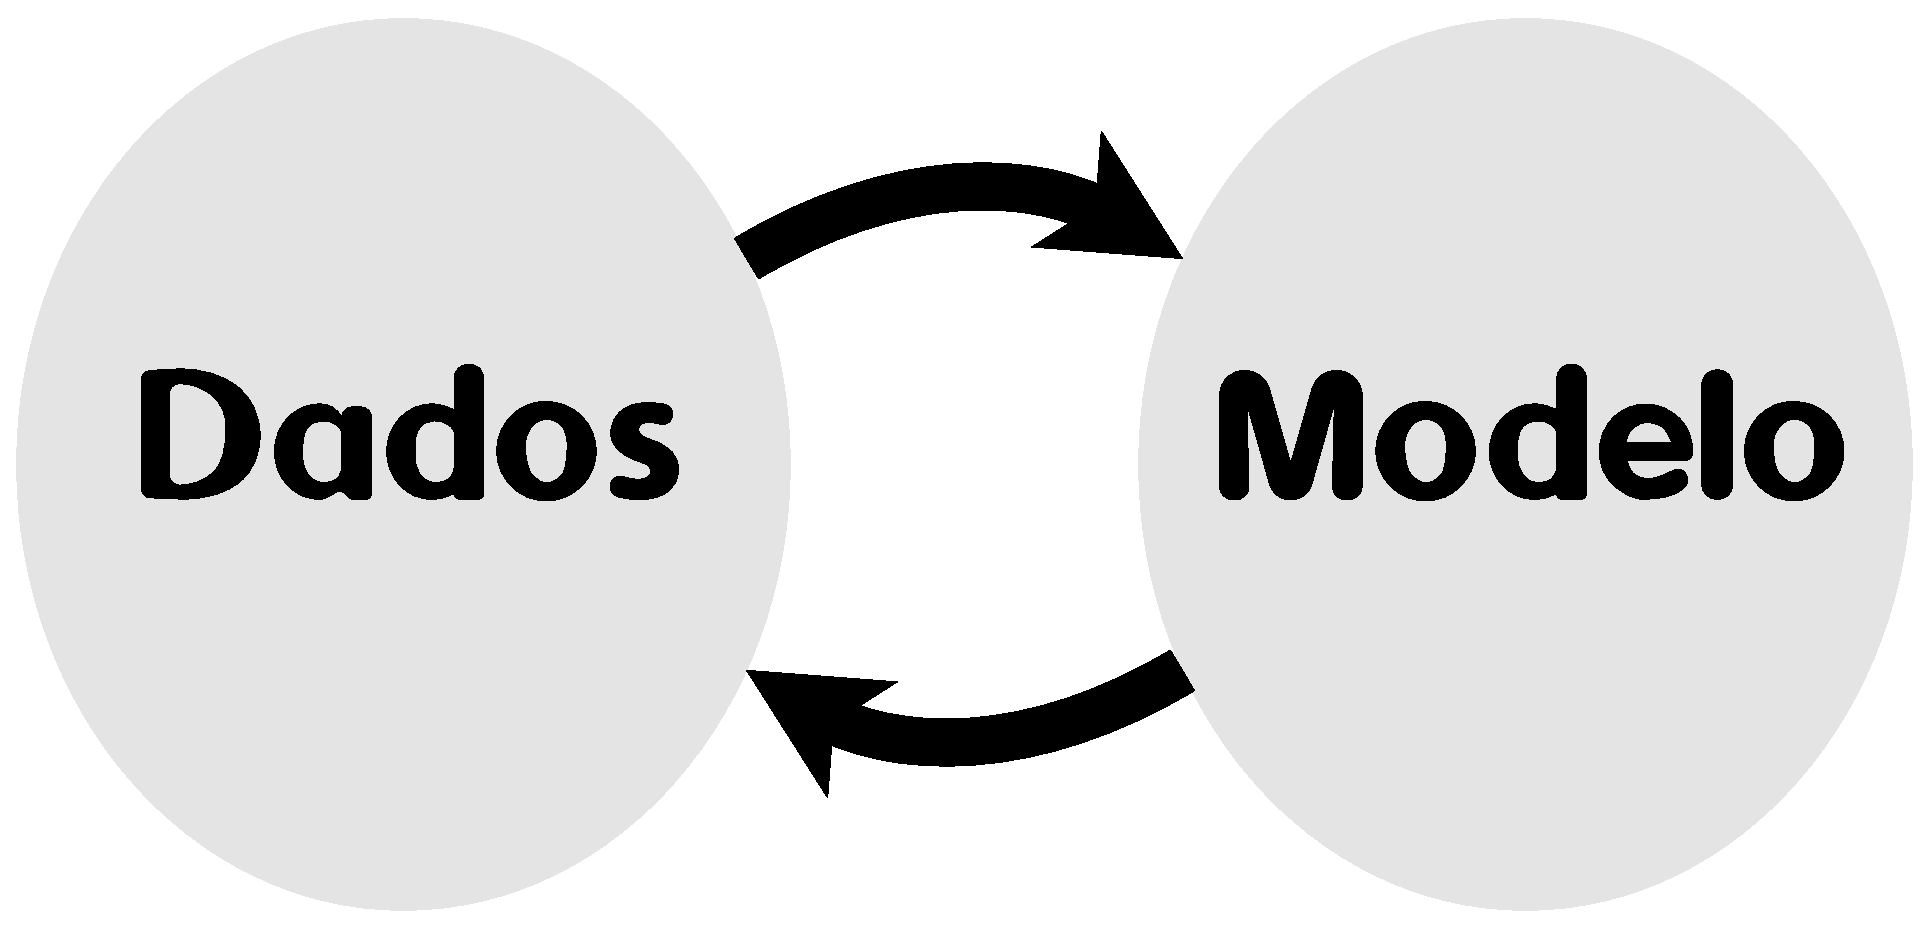
\includegraphics[width=0.6\textwidth]{principal}\\[1.0cm]
%% pretitle
%{\fontsize{25}{30} \textsc{Algum pretitulo}}
%% Title
\HRule{0.4cm} \\[0.4cm]
{ \fontsize{50}{60}   \bfseries \mytitle}\\[0.4cm]
\HRule{0.4cm} \\[0.7cm]
%% SubTitle
{\fontsize{25}{30} \textsc{\mysubtitle}}\\[0.5cm]
\vfill
%% Author 
\begin{minipage}{0.4\textwidth}
\begin{flushleft} \large
%\emph{Author:}\\
\myauthor %\textsc{Coppejans}
\end{flushleft}
\end{minipage}
% ID
\begin{minipage}{0.4\textwidth}
\begin{flushright} \large
\emph{email:} \\
\ImprimirEmail
\end{flushright}
\end{minipage}
% Bottom of the page
\vfill
{\large \imprimiryear}
\end{center}
\end{titlepage}
%% \end{comment}


%----------------------------------------------------------------------------------------
%	COPYRIGHT PAGE
%----------------------------------------------------------------------------------------
%\cleardoublepage

\newpage
\thispagestyle{empty}

\noindent Copyright \copyright\ \imprimiryear \myauthor\\ % Copyright notice

~\\

\noindent \textsc{Impresso no Brasil -- ISBN:\imprimirisbn}\\ % Publisher
\noindent \textsc{Publicado por \imprimireditora}\\ % Publisher
\noindent \textsc{Primeira impressão , \imprimirdata} % Printing/edition date

~\\

\textbf{Ficha catalográfica}
\begin{catalografica}%%
	\sffamily
	\vspace*{\fill}					% Posição vertical
	\begin{center}					% Minipage Centralizado
	\fbox{\begin{minipage}[c][5cm]{13.5cm}		% Largura
	\small
	\myauthor.
	%Sobrenome, Nome do autor
	
	\hspace{0.5cm} \mytitle: \mysubtitle   / \myauthor. --
	\imprimirlocal, \imprimiryear.
	
	\hspace{0.5cm} \pageref{LastPage} p. : il. (algumas color.) ; \imprimirsize.\\
	
	%\hspace{0.5cm} \imprimirorientadorRotulo~\imprimirorientador\\
	
	\hspace{0.5cm}
	\parbox[t]{\textwidth}{\imprimirtipotrabalho~--~\imprimireditora,~\imprimirdata.}\\

	\hspace{0.5cm}
	\parbox[t]{\textwidth}{ISBN:\imprimirisbn}\\


	
	\hspace{0.5cm}
		1. Samba de gafieira.
		2. Samba.
		3. Gafieira.
		4. Partitura de movimento.
        5. Musicalidade.
		I. Título 			
	\end{minipage}}
	\end{center}
\end{catalografica}%%

~\\

\noindent \textit{Garanta o ``download'' gratuito da versão digital do livro em \ImprimirLinkHomePageLivro}\\


\noindent Limite de responsabilidade e exceção de garantia: O autor ou autores tem feito
seu melhor esforço na preparação deste material.
Esta edição deve ser proporcionada sem nenhuma modificação. 
Se distribui gratuitamente com a esperança de que seja útil, 
porém sem nenhuma garantia expressa ou implícita em relação à exatidão ou completitude do conteúdo.


\vfill
\begin{wrapfigure}{l}{0.23\textwidth}
\includegraphics[height=32pt]{by-nc-nd.png}
\end{wrapfigure}
\noindent Esta obra está liberada com uma Licença 
Creative Commons Atribuição - NãoComercial - SemDerivações 4.0 Internacional.
Não é possível usar este arquivo excepto em conformidade com a Licença. 
Pode obter uma copia da Licença em:
\url{https://creativecommons.org/licenses/by-nc-nd/4.0/}\\ % License information


%----------------------------------------------------------------------------------------
%	DEDICATORIA
%----------------------------------------------------------------------------------------
\include{preliminares/dedicatoria} 

%----------------------------------------------------------------------------------------
%	Acknowledgements
%----------------------------------------------------------------------------------------
\cleardoublepage

\begin{center}
\Huge{\textbf{Agradecimentos}}
\end{center}

\null
\vfill
\thispagestyle{empty}

{\normalsize \it \hfill Dou muitas graças a Deus \vspace*{4pt}}


~\\

{\normalsize \it Dou muitas graças a XXXXX XXXXXXXXX por me 
ajudar a resolver muitas duvidas sobre definições e uso de termos na XXXXXXX XXXXXXX.
\vspace*{4pt}}

{\normalsize \it Dou muitas graças a XXXXX XXXXXXXXX por me 
ajudar a resolver muitas duvidas sobre definições e uso de termos na XXXXXXX XXXXXXX.
\vspace*{4pt}}

{\normalsize \it Dou muitas graças a XXXXX XXXXXXXXX por me 
ajudar a resolver muitas duvidas sobre definições e uso de termos na XXXXXXX XXXXXXX.
\vspace*{4pt}}


\begin{comment}
{\normalsize \it Dou muitas graças a \textcolor{red}{XXXXXXXXXXX} pela 
suas sugestões e revisão  do capitulo \textcolor{red}{XXXXXXXXXXX}.
\vspace*{4pt}}
\end{comment}


 

%----------------------------------------------------------------------------------------
%	PATROCINIO PAGE
%----------------------------------------------------------------------------------------
\cleardoublepage

\newpage
\thispagestyle{empty}


\begin{center}
\Huge{\textbf{Patrocínio}}
\end{center}

~\\

~\\



\begin{patrocinio}%%
	\sffamily
	\vspace*{\fill}					% Posição vertical
	\begin{center}					% Minipage Centralizado
	\fbox{\begin{minipage}[c][]{13.5cm}		% Largura

    ~\\

    \hspace{0.5cm}
    Para investir nesta pesquisa e colaborar com o desenvolvimento e crescimento deste projeto:
    \begin{itemize}
    \item Você pode comprar uma versão impressa do livro
    desde o seguinte endereço eletrônico:\\
    \ImprimirLinkCompraLivroImpresso 
    \item Você pode comprar uma versão digital desde:\\
    \ImprimirLinkCompraLivroDigital \\ 
    \end{itemize}


    \hspace{0.5cm}
    Também pode colaborar com dinheiro em efetivo, desde 20 reais (5 USD), 
    pelos seguintes métodos:
    \begin{itemize}
    \item Método 1
    \item Método 2 \\
    \end{itemize}


    \hspace{0.5cm} Para verificar a integridade do arquivo da versão digital deste livro,
    pode seguir as indicações publicadas no sitio oficial do projeto:\\
    \ImprimirLinkHomePageLivro\\

    \hspace{0.5cm}
    Se já colaborou com a pesquisa, e se assim o deseja, 
    sintase livre de me mandar um e-mail a \ImprimirEmail, 
    sugerindo abordar um novo assunto ou aprofundar em outro.
    Se seu pedido está dentro das minhas capacidades 
    este será agregado sem falta na seguinte edição do livro.\\

    \begin{flushright}
    \myauthor ~\\ 
    \end{flushright}

	\end{minipage}}
	\end{center}
\end{patrocinio}%%



%----------------------------------------------------------------------------------------
%	My macros
%----------------------------------------------------------------------------------------
%%%%%%%%%%%%%%%%%%%%%%%%%%%%%%%%%%%%%%%%%%%%%%%%%%%%%%%%%%%%%%%%%%%%%%%%%%%%%%%%
%%%%%%%%%%%%%%%%%%%%%%%%%%%%%%%%%%%%%%%%%%%%%%%%%%%%%%%%%%%%%%%%%%%%%%%%%%%%%%%%
%%%% Macros para equaçoes
%%%%%%%%%%%%%%%%%%%%%%%%%%%%%%%%%%%%%%%%%%%%%%%%%%%%%%%%%%%%%%%%%%%%%%%%%%%%%%%%

%% diagonal function
%\newcommand{\funcdiag}{diag}


%% vectorization function
\newcommand{\funcvec}{vec}

%% transpose function
\newcommand{\funcinv}{inv}

%% transpose function
\newcommand{\functrans}{trans}
%% transpose operator
\newcommand{\transpose}{\mathrm{T}}

%% block matrix
%\newcommand{\funcblockdiag}{blkdiag}
%\newcommand{\funcblockhor }{blkhorz}
%\newcommand{\funcblockver }{blkvert}


%% definiçao de tipos de arrays
\newcommand{\TRIX}[1]{\mathbf{\overline{\uppercase{#1}}}}
\newcommand{\MATRIX}[1]{\mathbf{\uppercase{#1}}}
\newcommand{\VECTOR}[1]{\mathbf{\lowercase{#1}}}

%%%%%%%%%%%%%%%%%%%%%%%%%%%%%%%%%%%%%%%%%%%%%%%%%%%%%%%%%%%%%%%%%%%%%%%%%%%%%%%%
%%%%%%%%%%%%%%%%%%%%%%%%%%%%%%%%%%%%%%%%%%%%%%%%%%%%%%%%%%%%%%%%%%%%%%%%%%%%%%%%
%%%% Macros para texto
%%%%%%%%%%%%%%%%%%%%%%%%%%%%%%%%%%%%%%%%%%%%%%%%%%%%%%%%%%%%%%%%%%%%%%%%%%%%%%%%

\newcommand{\FALTAPROVA}{\textcolor{red}{[FALTA PROVA!!!]}}
\newcommand{\FALTAREFERENCIA}{\textcolor{red}{[FALTA REFERENCIA!!!]}}


%----------------------------------------------------------------------------------------
%	TABLE OF CONTENTS
%----------------------------------------------------------------------------------------
\chapterimage{chapter_head_1_HSV.pdf} % Table of contents heading image
\pagestyle{empty} % No headers
%\pagestyle{fancy} % Print headers again
\tableofcontents % Print the table of contents itself
\cleardoublepage % Forces the first chapter to start on an odd page so it's on the right
\pagestyle{fancy} % Print headers again

%----------------------------------------------------------------------------------------
%	PART
%----------------------------------------------------------------------------------------
\part{Teoria geral}
% CHAPTER  
\chapterimage{chapter_head_2.pdf} % Chapter heading image

\chapter{Notação}


\begin{notation}Modo em que os valores escalares, vetoriais ou matriciais são definidos:\\
\begin{tabular}{r | p{.4\linewidth} | l}
\hline	
Tipo & Descrição & Formatação \\ \hline
$\mathbf{A}$, $\mathbf{B}$, ..., $\mathbf{X}$, $\mathbf{Y}$, $\mathbf{Z}$& Matriz. & Maiúsculo e negrito \\
$\mathbf{a}$, $\mathbf{b}$, ..., $\mathbf{x}$, $\mathbf{y}$, $\mathbf{z}$ & Vetor ou conjunto. & Minúsculo e negrito \\
%$A$, $B$, ..., $X$, $Y$, $Z$ & ------- & Maiúsculo \\
$a$, $b$, ..., $x$, $y$, $z$ & Escalar variável. & Minúsculo \\
$A$, $B$, ..., $X$, $Y$, $Z$ & Escalar constante. & Minúsculo \\
$\alpha$, $\beta$, ..., $\chi$, $\psi$, $\omega$ & Escalar variável ou constante. & Letras gregas e minúsculo  \\ \hline
\end{tabular}
\end{notation}

\begin{notation}Modo em que os elementos das matrizes bidimensionais são definidos:\\
\begin{tabular}{r | p{.6\linewidth} | l}
\hline	
Tipo & Descrição & Formatação \\ \hline
$a_{ij}$ & Escalar formado pelo elemento da linha $i$, coluna $j$ da matriz $\mathbf{A}$. & Minúsculo \\ \hline
%$\mathbf{A}_{(i,j)}$& Elemento na linha $i$, coluna $j$ da matriz $\mathbf{A}$ & Maiúsculo e negrito \\ \hline
%$\mathbf{a}_{i}$ & Linha ou coluna $i$-essima da matriz $\mathbf{A}$ (ambíguo) & Minúsculo e negrito \\
$a_{i:}$ & Vetor linha formado pela linha $i$-essima da matriz $\mathbf{A}$.  & Minúsculo \\
%$\mathbf{A}_{(i,:)}$& Vetor formado pela linha $i$-essima da matriz $\mathbf{A}$ & Maiúsculo e negrito \\
$a_{:i}$ & Vetor coluna formado pela coluna $i$-essima da matriz $\mathbf{A}$.  & Minúsculo \\
%$\mathbf{A}_{(:,i)}$& Vetor formado pela coluna $i$-essima da matriz $\mathbf{A}$ & Maiúsculo e negrito \\ \hline
\end{tabular}
\end{notation}

\begin{notation}Modo em que os elementos dos vetores ou conjuntos são definidos:\\
\begin{tabular}{r | p{.6\linewidth} | l}
\hline	
Tipo & Descrição & Formatação \\ \hline
$a_{i}$ & Elemento $i$-essimo do vetor ou conjunto  $\mathbf{a}$.& Minúsculo \\
%$\mathbf{a}_{(i)}$ & Elemento $i$-essimo do vetor $\mathbf{a}$ & Minúsculo e negrito \\ \hline
\end{tabular}
\end{notation}


\begin{notation}Funções notáveis usadas neste livro:\\
\begin{tabular}{r | l }
\hline	
Função & Descrição \\ \hline
$card(\mathbf{a})$ & Número de elementos, cardinalidade, do vetor ou conjunto $\mathbf{a}$. \\
$card(\mathbf{A})$ & Número de elementos, cardinalidade, da matriz $\mathbf{A}$. \\
\hline
$dim(\mathbf{a},1)$ & Primeira dimensão do vetor $\mathbf{a}$, número de linhas. \\
$dim(\mathbf{a},2)$ & Segunda dimensão do vetor $\mathbf{a}$, número de colunas. \\
$dim(\mathbf{A},1)$ & Primeira dimensão da matriz $\mathbf{A}$, número de linhas. \\
$dim(\mathbf{A},2)$ & Segunda dimensão da matriz $\mathbf{A}$, número de colunas. \\
$dim(\mathbf{A},N)$ & Dimensão $N$ da matriz $\mathbf{A}$, se não tiver retorna $0$. \\
\hline
$inv(\mathbf{A})$ & Inversa da matriz $\mathbf{A}$, é equivalente a escrever $\mathbf{A}^{-1}$. \\
$\mathbf{A}^{-1}$ & Inversa da matriz $\mathbf{A}$, é equivalente a escrever $inv(\mathbf{A})$. \\
\hline
$trans(\mathbf{a})$ & Transposta do vetor $\mathbf{a}$, é equivalente a escrever $\mathbf{a}^{T}$. \\
$\mathbf{a}^{T}$ & Transposta do vetor $\mathbf{a}$, é equivalente a escrever $trans(\mathbf{a})$. \\
$trans(\mathbf{A})$ & Transposta da matriz $\mathbf{A}$, é equivalente a escrever $\mathbf{A}^{T}$. \\
$\mathbf{A}^{T}$ & Transposta da matriz $\mathbf{A}$, é equivalente a escrever $trans(\mathbf{A})$. \\
\end{tabular}
\end{notation}


\chapterimage{chapter_matrix.pdf} % Chapter heading image


\chapter{Propriedades das matrizes}

%%%%%%%%%%%%%%%%%%%%%%%%%%%%%%%%%%%%%%%%%%%%%%%%%%%%%%%%%%%%%%%%%%%%%%%%%%%%%%%%%%%%%%%
%%%%%%%%%%%%%%%%%%%%%%%%%%%%%%%%%%%%%%%%%%%%%%%%%%%%%%%%%%%%%%%%%%%%%%%%%%%%%%%%%%%%%%%
%%%%%%%%%%%%%%%%%%%%%%%%%%%%%%%%%%%%%%%%%%%%%%%%%%%%%%%%%%%%%%%%%%%%%%%%%%%%%%%%%%%%%%%
\section{ Matrizes ortogonais}

\index{Matriz!Ortogonal}

\begin{definition}[Matriz ortogonal:]\label{def:ortogonalmatrix0}
Conhecida uma matriz quadrada $\MATRIX{A} \in \mathbb{R}^{N \times N}$. 
\begin{itemize}
\item Esta é uma matriz ortogonal quando se cumpre que \cite[pp. 66]{golub2013matrix}
\begin{equation}
\MATRIX{A}^{\transpose} = \MATRIX{A}^{-1}.
\end{equation}
\end{itemize}
\end{definition}

\begin{theorem}[Colunas da matriz ortogonal:]\label{theo:ortogonalmatrix0}
Conhecida uma matriz ortogonal $\MATRIX{Q} \in \mathbb{R}^{N \times N}$,
\begin{itemize}
\item A matriz $\MATRIX{Q}=\left[\VECTOR{q}_1\quad \VECTOR{q}_2\quad ... \quad \VECTOR{q}_N \right]$
está formada pela agrupação em colunas de um conjunto de $N$ vetores $\VECTOR{q}_n \in \mathbb{R}^{N}$
ortogonais \cite[pp. 66]{golub2013matrix}, onde 
\begin{equation}
\VECTOR{q}_i^{\transpose}\VECTOR{q}_j=
\left\{ 
\begin{matrix}
1 & se & i = j\\
0 & se & i \neq j
\end{matrix}
\right.
\end{equation} 
\end{itemize}
\end{theorem}



%%%%%%%%%%%%%%%%%%%%%%%%%%%%%%%%%%%%%%%%%%%%%%%%%%%%%%%%%%%%%%%%%%%%%%%%%%%%%%%%
%\newpage
%%%%%%%%%%%%%%%%%%%%%%%%%%%%%%%%%%%%%%%%%%%%%%%%%%%%%%%%%%%%%%%%%%%%%%%%%%%%%%%%%%%%%%%
%%%%%%%%%%%%%%%%%%%%%%%%%%%%%%%%%%%%%%%%%%%%%%%%%%%%%%%%%%%%%%%%%%%%%%%%%%%%%%%%%%%%%%%
%%%%%%%%%%%%%%%%%%%%%%%%%%%%%%%%%%%%%%%%%%%%%%%%%%%%%%%%%%%%%%%%%%%%%%%%%%%%%%%%%%%%%%%
\section{Propriedades varias com matrizes}


\begin{theorem}[Propiedades das matrices inversas:]\label{theo:matrixgeneric2}
Conhecidas as matrizes quadradas $\MATRIX{A} \in \mathbb{R}^{N \times N}$ e $\MATRIX{B} \in \mathbb{R}^{N \times N}$,
podemos afirmar \cite[pp. 65]{golub2013matrix},
\begin{itemize}
\item  A inversa da multiplicação de duas matrizes,
\begin{equation}
\MATRIX{A}^{-1} \MATRIX{B}^{-1} = \left\{\MATRIX{B}\MATRIX{A}\right\}^{-1}.
\end{equation}
\item A inversa da matriz transposta,
\begin{equation}
\left\{\MATRIX{A}^{-1}\right\}^{\transpose}  = \left\{\MATRIX{A}^{\transpose}\right\}^{-1}.
\end{equation}
\end{itemize}
\end{theorem}

\begin{theorem}[Propiedades com determinantes:]\label{theo:matrixgeneric1}
Conhecidas as matrizes quadradas $\MATRIX{A} \in \mathbb{R}^{N \times N}$ e $\MATRIX{B} \in \mathbb{R}^{N \times N}$,
e o escalar $\alpha \in \mathbb{R}$, podemos afirmar \cite[pp. 66]{golub2013matrix},
\begin{itemize}
\item Determinante da matriz transposta,
\begin{equation}
det(\MATRIX{A})=det(\MATRIX{A}^{\transpose}).
\end{equation}
\item Determinante da multiplicação de uma matriz e um escalar,
\begin{equation}
det(\alpha \MATRIX{A})=\alpha^N~det(\MATRIX{A}).
\end{equation}
\item Determinante da multiplicação de duas matrizes,
\begin{equation}
det(\MATRIX{A}\MATRIX{B})=det(\MATRIX{A})det(\MATRIX{B}).
\end{equation}
\end{itemize}
\end{theorem}


\begin{definition}[Autovalor e autovetores de uma matriz:]\label{def:matrixgeneric0}
Seja a matriz $\MATRIX{A}$ um operador linear $\MATRIX{A}: \mathbb{C}^{N} \rightarrow \mathbb{C}^{N}$,  
e $\VECTOR{v} \in \mathbb{C}^{N} \neq\VECTOR{0}$. Se existe um escalar $\lambda \in \mathbb{C}$ onde, 
%\begin{equation}
$\MATRIX{A}\VECTOR{v}=\lambda\VECTOR{v}$,
%\end{equation} 
então $\VECTOR{v}$ é um autovetor de $\MATRIX{A}$, e $\lambda$ é seu autovalor asociado.
\end{definition}


\begin{theorem}[Autovalor  na matriz transposta:]\label{theo:matrixgeneric3}
Conhecida uma matriz quadrada $\MATRIX{A} \in \mathbb{R}^{N \times N}$, 
com  autovalores $\lambda_n$, $\forall n \in \{1, 2, ..., N\}$.
%e autovetores $\VECTOR{e}_n$, $\forall n \in \{1, 2, ..., N\}$.
\begin{itemize}
\item A matriz $\MATRIX{A}^{\transpose}$ tem
\footnote{A demostração pode ser vista na Prova \ref{proof:theo:matrixgeneric3}.} 
os mesmos autovalores que $\MATRIX{A}$, é dizer tem o mesmo polinômio caraterístico $p(\lambda)$,
\begin{equation}
p(\lambda)=det(\MATRIX{A}-\lambda \MATRIX{I})=det(\MATRIX{A}^{\transpose}-\lambda \MATRIX{I}).
\end{equation}
\end{itemize}
\end{theorem}

%%%%%%%%%%%%%%%%%%%%%%%%%%%%%%%%%%%%%%%%%%%%%%%%%%%%%%%%%%%%%%%%%%%%%%%%%%%%%%%%
%\newpage
%%%%%%%%%%%%%%%%%%%%%%%%%%%%%%%%%%%%%%%%%%%%%%%%%%%%%%%%%%%%%%%%%%%%%%%%%%%%%%%%%%%%%%%
%%%%%%%%%%%%%%%%%%%%%%%%%%%%%%%%%%%%%%%%%%%%%%%%%%%%%%%%%%%%%%%%%%%%%%%%%%%%%%%%%%%%%%%
%%%%%%%%%%%%%%%%%%%%%%%%%%%%%%%%%%%%%%%%%%%%%%%%%%%%%%%%%%%%%%%%%%%%%%%%%%%%%%%%%%%%%%%
\section{ Matrizes semidefinidas positivas}
\index{Matriz!Semidefinida positiva}

\begin{definition}[Matriz semidefinida positiva:]\label{def:semipositivematrix0}
Conhecida uma matriz quadrada $\MATRIX{A} \in \mathbb{R}^{N \times N}$. 
\begin{itemize}
\item Esta é semidefinida positiva, se para todo non-zero vetor $\VECTOR{x} \in \mathbb{R}^N$
se cumpre que \cite[pp. 159]{golub2013matrix} 
\begin{equation}
\VECTOR{x}^{\transpose} \MATRIX{A} \VECTOR{x} \geq 0
\end{equation}
\end{itemize}
\end{definition}

~

\begin{theorem}[Matriz  $\MATRIX{A}^{\transpose}\MATRIX{A}$ e matrizes semidefinida positiva:]\label{theo:semipositivematrix1}
Conhecida uma matriz $\MATRIX{A} \in \mathbb{R}^{N \times M}$, 
\begin{itemize}
\item A matriz $\MATRIX{A}\MATRIX{A}^{\transpose} \geq \MATRIX{0}$ é
\footnote{A demostração pode ser vista na Prova \ref{proof:theo:semipositivematrix1}.} 
uma matriz semidefinida positiva.
\item Consequentemente, tambem a matriz $\MATRIX{A}^{\transpose}\MATRIX{A}  \geq \MATRIX{0}$ é semidefinida positiva.
\end{itemize}
\end{theorem}

~

\begin{theorem}[Autovalores e matrizes semidefinida positiva:]\label{theo:semipositivematrix2}
Conhecida uma matriz $\MATRIX{A} \in \mathbb{R}^{N \times N}$, com  autovalores $\lambda_n$,
$\forall n \in \{1, 2, ..., N\}$.
\begin{itemize}
\item Se a matriz $\MATRIX{A}$ é semidefinida positiva, então
\footnote{A demostração pode ser vista na Prova \ref{proof:theo:semipositivematrix2}.} 
os autovalores $\lambda_n \geq 0$.
\end{itemize}
\end{theorem}

%%%%%%%%%%%%%%%%%%%%%%%%%%%%%%%%%%%%%%%%%%%%%%%%%%%%%%%%%%%%%%%%%%%%%%%%%%%%%%%%
\newpage
%%%%%%%%%%%%%%%%%%%%%%%%%%%%%%%%%%%%%%%%%%%%%%%%%%%%%%%%%%%%%%%%%%%%%%%%%%%%%%%%%%%%%%%
%%%%%%%%%%%%%%%%%%%%%%%%%%%%%%%%%%%%%%%%%%%%%%%%%%%%%%%%%%%%%%%%%%%%%%%%%%%%%%%%%%%%%%%
%%%%%%%%%%%%%%%%%%%%%%%%%%%%%%%%%%%%%%%%%%%%%%%%%%%%%%%%%%%%%%%%%%%%%%%%%%%%%%%%%%%%%%%
\section{ Matrizes definidas positivas}

\index{Matriz!Definida positiva}

%%%%%%%%%%%%%%%%%%%%%%%%%%%%%%%%%%%%%%%%%%%%%%%%%%%%%%%%%%%%%%%%%%%%%%%%%%%%%%%%
\begin{definition}[Matriz definida positiva:]\label{def:positivematrix0}
Conhecida uma matriz quadrada $\MATRIX{A} \in \mathbb{R}^{N \times N}$. 
\begin{itemize}
\item Esta é definida positiva, se para todo vetor não nulo $\VECTOR{x} \in \mathbb{R}^N$
se cumpre que \cite[pp. 159]{golub2013matrix} 
\begin{equation}
\VECTOR{x}^{\transpose} \MATRIX{A} \VECTOR{x} > 0.
\end{equation}
\end{itemize}
\end{definition}




%%%%%%%%%%%%%%%%%%%%%%%%%%%%%%%%%%%%%%%%%%%%%%%%%%%%%%%%%%%%%%%%%%%%%%%%%%%%%%%%
\begin{theorem}[Autovalores positivos e matrizes definidas positivas:]\label{theo:positivematrix1}
Conhecida uma matriz quadrada $\MATRIX{A} \in \mathbb{R}^{N \times N}$, com  autovalores $\lambda_n$,
e autovetores $\VECTOR{e}_n$, $\forall n \in \{1, 2, ..., N\}$.
\begin{itemize}
\item Se $\MATRIX{A}$ é uma matriz definida positiva, então\footnote{\label{foot:theo:positivematrix1}A
demonstração pode ser vista na Prova \ref{proof:theo:positivematrix1}.}  
podemos afirmar que todos os autovalores 
\begin{equation}
\lambda_n > 0.
\end{equation}
\item Se todos os autovalores $\lambda_n$ são positivos e a matriz $\MATRIX{A}$ é \hyperref[def:symmetricmatrix0]{simétrica},
\begin{equation}
\lambda_n > 0 \qquad \wedge \qquad \MATRIX{A}=\MATRIX{A}^{\transpose},
\end{equation}
 então\footnote{A
demonstração pode ser vista na Prova \ref{proof:theo:positivematrix2}.} 
podemos afirmar que $\MATRIX{A}$ é uma matriz definida positiva.
\end{itemize}
\end{theorem}

\begin{tcbattention}
Conhecida uma matriz quadrada $\MATRIX{A} \in \mathbb{R}^{N \times N}$, 
com  autovalores $\lambda_n$, $\forall n \in \{1, 2, ..., N\}$.
\begin{itemize}
\item Que todos os autovalores $\lambda_n$ sejam positivos não garante que a matriz $\MATRIX{A}$
seja definida positiva. Para mais detalhes, ver o Exemplo \ref{ex:positivematrix1}.
\end{itemize}
\end{tcbattention}

%%%%%%%%%%%%%%%%%%%%%%%%%%%%%%%%%%%%%%%%%%%%%%%%%%%%%%%%%%%%%%%%%%%%%%%%%%%%%%%%
\noindent
\begin{minipage}{0.5\textwidth}
\begin{example}[Autovalores positivos não garantem matrizes definidas positivas:]
\label{ex:positivematrix1}
Conhecida uma matriz quadrada $\MATRIX{A}$ com autovalores positivos agrupados no vetor $\VECTOR{\lambda}_{\VECTOR{a}}$, 
\begin{equation}
\MATRIX{A}=
\begin{bmatrix}
1 & -8\\
0 & 2
\end{bmatrix}
\quad \rightarrow \quad 
\VECTOR{\lambda}_{\VECTOR{a}}=
\begin{bmatrix}
1 \\
2
\end{bmatrix}.
\end{equation}
Podemos verificar que a matriz $\MATRIX{A}$ não é definida positiva,
\begin{equation}
\VECTOR{x}=
\begin{bmatrix}
1 \\
1
\end{bmatrix}
\quad \rightarrow \quad 
-5 = \VECTOR{x}^{\transpose}\MATRIX{A}\VECTOR{x}<0.
\end{equation}
A superfície $\VECTOR{x}^{\transpose}\MATRIX{A}\VECTOR{x}$ 
pode ser vista na Figura \ref{fig:ex:positivematrix1}.
\end{example}
\end{minipage}
\begin{minipage}{0.5\textwidth}
     \begin{figure}[H]
         \centering
         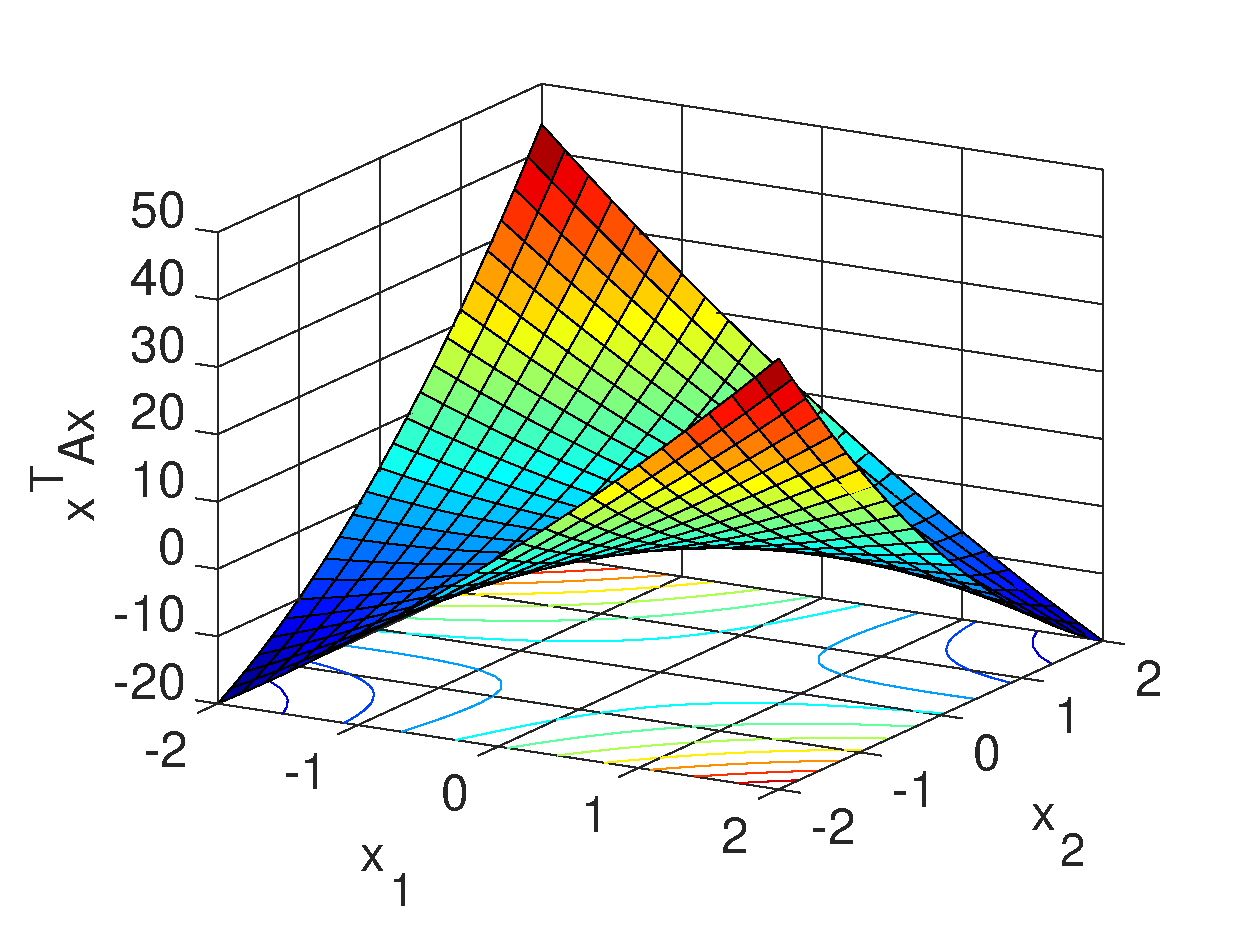
\includegraphics[width=0.98\textwidth]{chapters/teoria-basica/mfiles/positive-matrix/surfcexAx.eps}
         \caption{Superfície $\VECTOR{x}^{\transpose}\MATRIX{A}\VECTOR{x}$. }
         \label{fig:ex:positivematrix1}
     \end{figure}
\end{minipage}

%%%%%%%%%%%%%%%%%%%%%%%%%%%%%%%%%%%%%%%%%%%%%%%%%%%%%%%%%%%%%%%%%%%%%%%%%%%%%%%%
\begin{theorem}[Matriz inversa e matrizes definidas positivas:]\label{theo:positivematrix:2}
Conhecida uma matriz  $\MATRIX{A} \in \mathbb{R}^{N \times N}$, com  autovalores $\lambda_n$,
$\forall n \in \{1, 2, ..., N\}$.
\begin{itemize}
\item Se $\MATRIX{A}$ é uma matriz simétrica e definida positiva, então\footnote{A
demonstração pode ser vista na Prova \ref{proof:theo:positivematrix:2}.}  
a matriz $\MATRIX{A}^{-1}$ tambem é definida positiva.
\end{itemize}
\end{theorem}


%%%%%%%%%%%%%%%%%%%%%%%%%%%%%%%%%%%%%%%%%%%%%%%%%%%%%%%%%%%%%%%%%%%%%%%%%%%%%%%%
\newpage
%%%%%%%%%%%%%%%%%%%%%%%%%%%%%%%%%%%%%%%%%%%%%%%%%%%%%%%%%%%%%%%%%%%%%%%%%%%%%%%%%%%%%%%
%%%%%%%%%%%%%%%%%%%%%%%%%%%%%%%%%%%%%%%%%%%%%%%%%%%%%%%%%%%%%%%%%%%%%%%%%%%%%%%%%%%%%%%
%%%%%%%%%%%%%%%%%%%%%%%%%%%%%%%%%%%%%%%%%%%%%%%%%%%%%%%%%%%%%%%%%%%%%%%%%%%%%%%%%%%%%%%
\section{Matrizes semelhantes}

\index{Matriz!Semelhante}

\begin{definition}[Matrizes semelhantes:]\label{def:similhante0}
Conhecidas as matrizes  $\MATRIX{A} \in \mathbb{C}^{N \times N}$ e $\MATRIX{B} \in \mathbb{R}^{N \times N}$,
estas são chamadas semelhantes \cite[pp. 67]{golub2013matrix} se existe uma matriz $\MATRIX{P} \in \mathbb{C}^{N \times N}$, que provoque
\begin{equation}
\MATRIX{A} = \MATRIX{P}^{-1} \MATRIX{B} \MATRIX{P}.
\end{equation}
\end{definition}

\begin{theorem}[Autovalores em matrizes semelhantes:]\label{theo:similhante1}
Conhecidas as matrizes $\MATRIX{A} \in \mathbb{C}^{N \times N}$ e $\MATRIX{B} \in \mathbb{R}^{N \times N}$,
\begin{itemize}
\item Se as matrizes $\MATRIX{A}$ e $\MATRIX{B}$ são semelhantes, então estas têm os mesmos autovalores
\footnote{A demostração pode ser vista na Prova \ref{proof:theo:similhante1}.} \cite[pp. 67]{golub2013matrix}.
\end{itemize}
\end{theorem}

%%%%%%%%%%%%%%%%%%%%%%%%%%%%%%%%%%%%%%%%%%%%%%%%%%%%%%%%%%%%%%%%%%%%%%%%%%%%%%%%%%%%%%%
%%%%%%%%%%%%%%%%%%%%%%%%%%%%%%%%%%%%%%%%%%%%%%%%%%%%%%%%%%%%%%%%%%%%%%%%%%%%%%%%%%%%%%%
%%%%%%%%%%%%%%%%%%%%%%%%%%%%%%%%%%%%%%%%%%%%%%%%%%%%%%%%%%%%%%%%%%%%%%%%%%%%%%%%%%%%%%%
\section{Diagonalização de matrizes}
\index{Matriz!Diagonalizável}

\begin{definition}[Matriz diagonalizável:]\label{def:diagonalization0}
Conhecida uma matriz quadrada $\MATRIX{A} \in \mathbb{R}^{N \times N}$ com
autovalores $\lambda_n$, $\forall n \in \{1, 2, ..., N\}$.
\begin{itemize}
\item Esta é definida como diagonalizável se é semelhante a uma matriz diagonal \cite[pp. 67]{golub2013matrix};
é dizer, existe uma matriz $\MATRIX{P}$ que provoca
\begin{equation}
\lambda_\MATRIX{A}\equiv
\begin{bmatrix}
\lambda_1 & 0         & ...    & 0 \\
0         & \lambda_2 & ...    & 0 \\
\vdots    & \vdots    & \ddots & \vdots \\
0         & 0         & ...    & \lambda_N
\end{bmatrix}
=\MATRIX{P}^{-1}\MATRIX{A}\MATRIX{P}.
\end{equation}
\end{itemize}
\end{definition}

~

\begin{theorem}[Diagonalização de matrizes:]\label{theo:diagonalization1}
Conhecida uma matriz quadrada $\MATRIX{A} \in \mathbb{R}^{N \times N}$ com
autovalores $\lambda_n$, $\forall n \in \{1, 2, ..., N\}$.
\begin{itemize}
\item Se $\MATRIX{A}$ tem $N$  autovetores $\VECTOR{v}_n \in \mathbb{R}^{N}$  linearmente independentes.
Então $\MATRIX{A}$ é diagonalizável \cite[pp. 159]{golub2013matrix};
com
\begin{equation}
\begin{bmatrix}
\lambda_1 & 0         & ...    & 0 \\
0         & \lambda_2 & ...    & 0 \\
\vdots    & \vdots    & \ddots & \vdots \\
0         & 0         & ...    & \lambda_N
\end{bmatrix}
=\MATRIX{V}^{-1}\MATRIX{A}\MATRIX{V},
\end{equation}
onde $\MATRIX{V}=\left[\VECTOR{v}_1\quad \VECTOR{v}_2\quad \VECTOR{v}_3\quad ...\quad \VECTOR{v}_N\right]$.

\item Se $\MATRIX{A}$ é uma matriz simétrica então
existe uma matriz $\MATRIX{Q}$ ortogonal que cumpre \cite[pp. 67, 440]{golub2013matrix};
com
\begin{equation}
\begin{bmatrix}
\lambda_1 & 0         & ...    & 0 \\
0         & \lambda_2 & ...    & 0 \\
\vdots    & \vdots    & \ddots & \vdots \\
0         & 0         & ...    & \lambda_N
\end{bmatrix}
=\MATRIX{Q}^{-1}\MATRIX{A}\MATRIX{Q},
\end{equation}
onde $\MATRIX{Q}=\left[\VECTOR{q}_1\quad \VECTOR{q}_2\quad \VECTOR{q}_3\quad ...\quad \VECTOR{q}_N\right]$,
e $\VECTOR{q}_i^{\transpose}\VECTOR{q}_j$ é igual $1$ quando $i=j$ e zero em outros casos.
\end{itemize}
\end{theorem}

%%%%%%%%%%%%%%%%%%%%%%%%%%%%%%%%%%%%%%%%%%%%%%%%%%%%%%%%%%%%%%%%%%%%%%%%%%%%%%%%
\newpage
%%%%%%%%%%%%%%%%%%%%%%%%%%%%%%%%%%%%%%%%%%%%%%%%%%%%%%%%%%%%%%%%%%%%%%%%%%%%%%%%%%%%%%%
%%%%%%%%%%%%%%%%%%%%%%%%%%%%%%%%%%%%%%%%%%%%%%%%%%%%%%%%%%%%%%%%%%%%%%%%%%%%%%%%%%%%%%%
%%%%%%%%%%%%%%%%%%%%%%%%%%%%%%%%%%%%%%%%%%%%%%%%%%%%%%%%%%%%%%%%%%%%%%%%%%%%%%%%%%%%%%%
\section{ Matrizes simétricas}

\index{Matriz!Simétrica}

\begin{definition}[Matriz simétrica:]\label{def:symmetricmatrix0}
Conhecida uma matriz quadrada $\MATRIX{A} \in \mathbb{R}^{N \times N}$. 
\begin{itemize}
\item Esta é uma matriz simétrica, sim se cumpre que \cite[pp. 18]{golub2013matrix} 
\begin{equation}
\MATRIX{A}^{\transpose} = \MATRIX{A}
\end{equation}
\end{itemize}
\end{definition}

\begin{theorem}[Forma quadratica e matrizes simétricas:]\label{theo:simetricmatrix0}
Conhecida uma matriz quadrada $\MATRIX{A} \in \mathbb{R}^{N \times N}$.
\begin{itemize}
\item Se definimos a matriz simétrica $\MATRIX{S}=\frac{\MATRIX{A}+\MATRIX{A}^{\transpose}}{2}$ então\footnote{A
demostração pode ser vista na Prova \ref{proof:theo:simetricmatrix0}.} 
podemos afirmar que para qualquer vetor $\VECTOR{x} \in \mathbb{R}^{N}$ se cumpre que 
\begin{equation}
\VECTOR{x}^{\transpose}\MATRIX{S}\VECTOR{x} = 
\VECTOR{x}^{\transpose}\MATRIX{A}\VECTOR{x} =
\VECTOR{x}^{\transpose}\MATRIX{A}^{\transpose}\VECTOR{x}
\end{equation}
\end{itemize}
\end{theorem}



\begin{theorem}[As matrizes simétricas são diagonalizaveis:]\label{theo:simetricmatrix2}
Conhecida uma matriz quadrada $\MATRIX{A} \in \mathbb{R}^{N \times N}$, 
com  autovalores $\lambda_n$, $\forall n \in \{1, 2, ..., N\}$.
%e autovetores $\VECTOR{e}_n$, $\forall n \in \{1, 2, ..., N\}$.
\begin{itemize}
\item Se $\MATRIX{A}$ é uma matriz simétrica então
%\footnote{A demostração pode ser vista na Prova \ref{proof:theo:simetricmatrix2}.} 
existe uma matriz $\MATRIX{Q}$ ortogonal que cumpre \cite[pp. 67,440]{golub2013matrix}
\begin{equation}
\begin{bmatrix}
\lambda_1 & 0         & ...    & 0 \\
0         & \lambda_2 & ...    & 0 \\
\vdots    & \vdots    & \ddots & \vdots \\
0         & 0         & ...    & \lambda_N
\end{bmatrix}
=\MATRIX{Q}^{-1}\MATRIX{A}\MATRIX{Q}.
\end{equation}
\end{itemize}
\end{theorem}


\begin{theorem}[Autovalor de maior valor em matrizes simétricas:]\label{theo:simetricmatrix3}
Conhecida uma matriz quadrada $\MATRIX{A} \in \mathbb{R}^{N \times N}$, 
com  autovalores $\lambda_n$, $\forall n \in \{1, 2, ..., N\}$.
%e autovetores $\VECTOR{e}_n$, $\forall n \in \{1, 2, ..., N\}$.
\begin{itemize}
\item Se $\MATRIX{A}$ é uma matriz simétrica então, $\lambda_{max}(\MATRIX{A})$,
o autovalor de maior valor da  matriz $\MATRIX{A}$ cumpre \cite[pp. 67]{golub2013matrix}
\begin{equation}
\lambda_{max}(\MATRIX{A}) = \max_{\VECTOR{x}\neq 0} \frac{\VECTOR{x}^{\transpose}\MATRIX{A}\VECTOR{x}}{\VECTOR{x}^{\transpose}\VECTOR{x}},
\end{equation}
\end{itemize}
onde $\VECTOR{x} \in \mathbb{R}^N$.
\end{theorem}

\begin{theorem}[Autovalor de menor valor em matrizes simétricas:]\label{theo:simetricmatrix4}
Conhecida uma matriz quadrada $\MATRIX{A} \in \mathbb{R}^{N \times N}$, 
com  autovalores $\lambda_n$, $\forall n \in \{1, 2, ..., N\}$.
%e autovetores $\VECTOR{e}_n$, $\forall n \in \{1, 2, ..., N\}$.
\begin{itemize}
\item Se $\MATRIX{A}$ é uma matriz simétrica então, $\lambda_{min}(\MATRIX{A})$,
o autovalor de menor valor da  matriz $\MATRIX{A}$ cumpre \cite[pp. 67]{golub2013matrix}
\begin{equation}
\lambda_{min}(\MATRIX{A}) = \min_{\VECTOR{x}\neq 0} \frac{\VECTOR{x}^{\transpose}\MATRIX{A}\VECTOR{x}}{\VECTOR{x}^{\transpose}\VECTOR{x}},
\end{equation}
onde $\VECTOR{x} \in \mathbb{R}^N$.
\end{itemize}
\end{theorem}

%%%%%%%%%%%%%%%%%%%%%%%%%%%%%%%%%%%%%%%%%%%%%%%%%%%%%%%%%%%%%%%%%%%%%%%%%%%%%%%%
\newpage
\section{Provas dos teoremas}

%%%%%%%%%%%%%%%%%%%%%%%%%%%%%%%%%%%%%%%%%%%%%%%%%%%%%%%%%%%%%%%%%%%%%%%%%%%%%%%%%%%%%%%
%%%%%%%%%%%%%%%%%%%%%%%%%%%%%%%%%%%%%%%%%%%%%%%%%%%%%%%%%%%%%%%%%%%%%%%%%%%%%%%%%%%%%%%
\begin{myproofT}[Prova do Teorema \ref{theo:simetricmatrix0}:]\label{proof:theo:simetricmatrix0}
Conhecida uma matriz quadrada $\MATRIX{A} \in \mathbb{R}^{N \times N}$,
Se definimos a matriz simétrica $\MATRIX{S}=\frac{\MATRIX{A}+\MATRIX{A}^{\transpose}}{2}$ e
o vetor $\VECTOR{x} \in \mathbb{R}^{N}$, então
\begin{equation}
\VECTOR{x}^{\transpose}\MATRIX{S}\VECTOR{x} = 
\frac{\VECTOR{x}^{\transpose}\MATRIX{A}\VECTOR{x}}{2} +
\frac{\VECTOR{x}^{\transpose}\MATRIX{A}^{\transpose}\VECTOR{x}}{2}
\end{equation}
dado que cada somando da equação anterior é um escalar podemos afirmar que 
\begin{equation}
\VECTOR{x}^{\transpose}\MATRIX{S}\VECTOR{x} = 
\frac{\VECTOR{x}^{\transpose}\MATRIX{A}\VECTOR{x}}{2} +
\left[\frac{\VECTOR{x}^{\transpose}\MATRIX{A}^{\transpose}\VECTOR{x}}{2}\right]^{\transpose}
\end{equation}
e consequentemente que
\begin{equation}
\VECTOR{x}^{\transpose}\MATRIX{S}\VECTOR{x} = 
\VECTOR{x}^{\transpose}\MATRIX{A}\VECTOR{x} =
\VECTOR{x}^{\transpose}\MATRIX{A}^{\transpose}\VECTOR{x}
\end{equation} 
\end{myproofT}

%%%%%%%%%%%%%%%%%%%%%%%%%%%%%%%%%%%%%%%%%%%%%%%%%%%%%%%%%%%%%%%%%%%%%%%%%%%%%%%%%%%%%%%
%%%%%%%%%%%%%%%%%%%%%%%%%%%%%%%%%%%%%%%%%%%%%%%%%%%%%%%%%%%%%%%%%%%%%%%%%%%%%%%%%%%%%%%
\begin{myproofT}[Prova do Teorema \ref{theo:positivematrix1}:]\label{proof:theo:positivematrix1}
Conhecida uma matriz quadrada $\MATRIX{A} \in \mathbb{R}^{N \times N}$ e definida positiva, com  autovalores $\lambda_n$,
e autovetores $\VECTOR{e}_n$, $\forall n \in \{1, 2, ..., N\}$, de modo que,
\begin{equation}\label{eq:proof:theo:positivematrix1:0}
\MATRIX{A}\VECTOR{e}_n=\lambda_n \VECTOR{e}_n.
\end{equation}
\begin{equation}\label{eq:proof:theo:positivematrix1:1}
\VECTOR{e}_n^{\transpose}\MATRIX{A}\VECTOR{e}_n=\lambda_n \VECTOR{e}_n^{\transpose}\VECTOR{e}_n.
\end{equation}

\begin{itemize}
\item Assim, usando a Eq. (\ref{eq:proof:theo:positivematrix1:1}) e a Definição \ref{def:positivematrix0} podemos afirmar que
\begin{equation}
\VECTOR{e}_n^{\transpose}\MATRIX{A}\VECTOR{e}_n >0
\end{equation} 
o que implica que
\begin{equation}
\lambda_n \VECTOR{e}_n^{\transpose}\VECTOR{e}_n > 0
\quad \rightarrow \quad
\lambda_n  \geq 0
\end{equation} 
\end{itemize}
\end{myproofT}


%%%%%%%%%%%%%%%%%%%%%%%%%%%%%%%%%%%%%%%%%%%%%%%%%%%%%%%%%%%%%%%%%%%%%%%%%%%%%%%%%%%%%%%
%%%%%%%%%%%%%%%%%%%%%%%%%%%%%%%%%%%%%%%%%%%%%%%%%%%%%%%%%%%%%%%%%%%%%%%%%%%%%%%%%%%%%%%
\begin{myproofT}[Prova do Teorema \ref{theo:positivematrix1}:]\label{proof:theo:positivematrix2}
Conhecida uma matriz quadrada $\MATRIX{A} \in \mathbb{R}^{N \times N}$ simetricas,
com  autovalores $\lambda_n>0$, $\forall n \in \{1, 2, ..., N\}$;
sabemos pelo Teorema \ref{theo:simetricmatrix2}, 
que existe uma \hyperref[def:ortogonalmatrix0]{\textbf{matriz ortogonal}} $\MATRIX{Q}$,
\begin{equation}
\MATRIX{Q}^{\transpose}\MATRIX{A}\MATRIX{Q} = \MATRIX{\lambda}_{\MATRIX{A}}\equiv
\begin{bmatrix}
\lambda_1 & 0         & ...    & 0 \\
0         & \lambda_2 & ...    & 0 \\
\vdots    & \vdots    & \ddots & \vdots \\
0         & 0         & ...    & \lambda_N
\end{bmatrix}.
\end{equation}
Se multiplicamos esta igualdade por um vector $\VECTOR{x} \in \mathbb{R}^N$ (non-zero), obtemos,
\begin{equation}
\VECTOR{x}^{\transpose} \MATRIX{Q}^{\transpose}\MATRIX{A}\MATRIX{Q} \VECTOR{x} = 
\VECTOR{x}^{\transpose} \MATRIX{\lambda}_{\MATRIX{A}} \VECTOR{x}
\end{equation}
\begin{equation}
\VECTOR{x}^{\transpose} \MATRIX{Q}^{\transpose}\MATRIX{A}\MATRIX{Q} \VECTOR{x} 
= \sum \limits_{n=1}^{N}\lambda_n x_n^2.
\end{equation}
Aplicando uma troca de variaveis de modo que $\VECTOR{y}=\MATRIX{Q} \VECTOR{x}$,
\begin{equation}
\VECTOR{y}^{\transpose} \MATRIX{A} \VECTOR{y} 
= \sum \limits_{n=1}^{N}\lambda_n x_n^2.
\end{equation}
Dado que a soma de todos os $\lambda_n x_n^2$ é positiva, podemos afirmar que
\begin{equation}
\VECTOR{y}^{\transpose} \MATRIX{A} \VECTOR{y} > 0;
\end{equation}
é dizer $\MATRIX{A}$ é definida positiva.
\end{myproofT}

%%%%%%%%%%%%%%%%%%%%%%%%%%%%%%%%%%%%%%%%%%%%%%%%%%%%%%%%%%%%%%%%%%%%%%%%%%%%%%%%%%%%%%%
%%%%%%%%%%%%%%%%%%%%%%%%%%%%%%%%%%%%%%%%%%%%%%%%%%%%%%%%%%%%%%%%%%%%%%%%%%%%%%%%%%%%%%%
\begin{myproofT}[Prova do Teorema \ref{theo:similhante1}:]\label{proof:theo:similhante1}
Conhecidas as matrizes semelhantes $\MATRIX{A} \in \mathbb{C}^{N \times N}$ e $\MATRIX{B} \in \mathbb{R}^{N \times N}$,
de modo que se cumpre que 
\begin{equation}
\MATRIX{A} = \MATRIX{P}^{-1} \MATRIX{B} \MATRIX{P}.
\end{equation}
para um $\MATRIX{P}$ dado.

Se calculamos o polinômio carateristico $p_{\MATRIX{A}}(\lambda)$ de $\MATRIX{A}$,
\begin{equation}
p_{\MATRIX{A}}(\lambda)=det\left(A-\lambda \MATRIX{I}\right),
\end{equation}
podemos rescrever esta equação
\begin{equation}
p_{\MATRIX{A}}(\lambda)=det\left(\MATRIX{P}^{-1} \MATRIX{B} \MATRIX{P}-\lambda \MATRIX{P}^{-1} \MATRIX{I} \MATRIX{P} \right),
\end{equation}
\begin{equation}
p_{\MATRIX{A}}(\lambda)=det\left( \MATRIX{P}^{-1}\right)det\left( \MATRIX{B} -\lambda \MATRIX{I} \right)det\left( \MATRIX{P}\right),
\end{equation}
\begin{equation}
p_{\MATRIX{A}}(\lambda)=det\left( \MATRIX{B} -\lambda \MATRIX{I} \right) = p_{\MATRIX{B}}(\lambda),
\end{equation}
\end{myproofT}




%----------------------------------------------------------------------------------------
%	PART
%----------------------------------------------------------------------------------------
\part{Funções, derivadas e operadores}
% CHAPTER  
\chapterimage{chapter_function.pdf} % Chapter heading image

\chapter{Funções e operadores notáveis}

%%%%%%%%%%%%%%%%%%%%%%%%%%%%%%%%%%%%%%%%%%%%%%%%%%%%%%%%%%%%%%%%%%%%%%%%%%%%%%%%
%\newpage
%%%%%%%%%%%%%%%%%%%%%%%%%%%%%%%%%%%%%%%%%%%%%%%%%%%%%%%%%%%%%%%%%%%%%%%%%%%%%%%%%%%%%%%
%%%%%%%%%%%%%%%%%%%%%%%%%%%%%%%%%%%%%%%%%%%%%%%%%%%%%%%%%%%%%%%%%%%%%%%%%%%%%%%%%%%%%%%
%%%%%%%%%%%%%%%%%%%%%%%%%%%%%%%%%%%%%%%%%%%%%%%%%%%%%%%%%%%%%%%%%%%%%%%%%%%%%%%%%%%%%%%
\section{Mnemônico vetor nabla $\vec{\triangledown}$}

\begin{notation}[Uso do Mnemônico vetor nabla 
($\overrightarrow{\triangledown}$ ):]
Dado um vetor coluna $\VECTOR{x}\in \mathbb{R}^N$, usaremos o mnemônico\footnote{Falando de um modo rigoroso, 
 $\overrightarrow{\triangledown}$ não é um operador diferencial, 
e sim um mnemônico que nos ajuda a lembrar e representar uma série de operadores diferenciais.} 
vetorial nabla ($\overrightarrow{\triangledown}$), como:
\begin{equation}
\overrightarrow{\triangledown}  \equiv \frac{\partial }{\partial \VECTOR{x}} =
\begin{bmatrix}
\frac{\partial  }{\partial x_{1}}\\
\frac{\partial  }{\partial x_{2}}\\
\vdots\\
\frac{\partial  }{\partial x_{n}}\\
\vdots\\
\frac{\partial  }{\partial x_{N}}
\end{bmatrix}
\end{equation}
\end{notation}
~

\begin{tcbattention}
Não deve ser confundido o mnemônico $\overrightarrow{\triangledown}$, 
com o operador $\triangledown$, cujo uso será explicado nas seguintes seções.
\end{tcbattention}
~

\begin{definition}[Derivada 
$\overrightarrow{\triangledown}^{\transpose}\VECTOR{f}(\VECTOR{x})$:]
\label{def:nabla:dot}
Dado 
um vetor coluna $\VECTOR{x}\in \mathbb{R}^N$ e 
uma função vetor coluna $\VECTOR{f}(\VECTOR{x}): \mathbb{R}^N \rightarrow \mathbb{R}^M$, 
definimos que:
\begin{equation}
\overrightarrow{\triangledown}.~\VECTOR{f}(\VECTOR{x}) \equiv
\overrightarrow{\triangledown}^{\transpose}\VECTOR{f}(\VECTOR{x})= 
\frac{\partial f_{1}(\VECTOR{x}) }{\partial x_{1}}+
\frac{\partial f_{2}(\VECTOR{x}) }{\partial x_{2}}+
\hdots+
\frac{\partial f_{n}(\VECTOR{x}) }{\partial x_{n}}+
\hdots+
\frac{\partial f_{N}(\VECTOR{x}) }{\partial x_{N}}=
\sum \limits_{n=1}^N \frac{\partial f_{n}(\VECTOR{x}) }{\partial x_{n}}
\end{equation}

\end{definition}


%%%%%%%%%%%%%%%%%%%%%%%%%%%%%%%%%%%%%%%%%%%%%%%%%%%%%%%%%%%%%%%%%%%%%%%%%%%%%%%%
\newpage

%%%%%%%%%%%%%%%%%%%%%%%%%%%%%%%%%%%%%%%%%%%%%%%%%%%%%%%%%%%%%%%%%%%%%%%%%%%%%%%%%%%%%%%
%%%%%%%%%%%%%%%%%%%%%%%%%%%%%%%%%%%%%%%%%%%%%%%%%%%%%%%%%%%%%%%%%%%%%%%%%%%%%%%%%%%%%%%
%%%%%%%%%%%%%%%%%%%%%%%%%%%%%%%%%%%%%%%%%%%%%%%%%%%%%%%%%%%%%%%%%%%%%%%%%%%%%%%%%%%%%%%
\section{Operador derivada para $e(\VECTOR{x})$, $\VECTOR{f}(\VECTOR{x})$ e  $\MATRIX{G}(\VECTOR{x})$}

%%%%%%%%%%%%%%%%%%%%%%%%%%%%%%%%%%%%%%%%%%%%%%%%%%%%%%%%%%%%%%%%%%%%%%%%%%%%%%%%
\subsection{Derivadas com respeito a $\VECTOR{x}^{\transpose}$}

\begin{definition}[Derivada de 
$e(\VECTOR{x})$ com respeito de $\VECTOR{x}^{\transpose}$:]\label{def:deltahor}
Dado 
um vetor coluna $\VECTOR{x}\in \mathbb{R}^N$ e 
uma função $e(\VECTOR{x}): \mathbb{R}^N \rightarrow \mathbb{R}$,
definimos que:
\begin{equation}
\left[\overrightarrow{\triangledown} e(\VECTOR{x})\right]^{\transpose} \equiv 
\frac{\partial e(\VECTOR{x}) }{\partial \VECTOR{x}^{\transpose}}= 
\left[
\begin{matrix}
\frac{\partial e(\VECTOR{x}) }{\partial x_{1}}&
\frac{\partial e(\VECTOR{x}) }{\partial x_{2}}&
\hdots&
\frac{\partial e(\VECTOR{x}) }{\partial x_{n}}&
\hdots&
\frac{\partial e(\VECTOR{x}) }{\partial x_{N}}
\end{matrix}
\right]= {\bigcup\limits_{n=1}^{\rightarrow}}^{N}{\frac{\partial e(\VECTOR{x}) }{\partial x_{n}}} 
\end{equation}
\end{definition}

\begin{definition}[Derivada de 
$\VECTOR{f}(\VECTOR{x})$ com respeito de $\VECTOR{x}^{\transpose}$:]\label{def:deltahor2}
Dado 
um vetor coluna $\VECTOR{x}\in \mathbb{R}^N$ e 
uma função vetor coluna $\VECTOR{f}(\VECTOR{x}): \mathbb{R}^N \rightarrow \mathbb{R}^M$, 
definimos que:
\begin{equation}
\left[\overrightarrow{\triangledown} \VECTOR{f}^{\transpose}(\VECTOR{x})\right]^{\transpose} \equiv 
\frac{\partial \VECTOR{f}(\VECTOR{x}) }{\partial \VECTOR{x}^{\transpose}}= 
\left[
\begin{matrix}
\frac{\partial \VECTOR{f}(\VECTOR{x}) }{\partial x_{1}}&
\frac{\partial \VECTOR{f}(\VECTOR{x}) }{\partial x_{2}}&
\hdots&
\frac{\partial \VECTOR{f}(\VECTOR{x}) }{\partial x_{n}}&
\hdots&
\frac{\partial \VECTOR{f}(\VECTOR{x}) }{\partial x_{N}}
\end{matrix}
\right]= {\bigcup\limits_{n=1}^{\rightarrow}}^{N}{\frac{\partial \VECTOR{f}(\VECTOR{x}) }{\partial x_{n}}} 
\end{equation}
\end{definition}

\begin{definition}[Derivada de 
$\MATRIX{G}(\VECTOR{x})$ com respeito de $\VECTOR{x}^{\transpose}$:]\label{def:deltahor3}
Dado 
um vetor coluna $\VECTOR{x}\in \mathbb{R}^N$ e 
uma função $\MATRIX{G}(\VECTOR{x}): \mathbb{R}^N \rightarrow \mathbb{R}^{M\times L}$, 
definimos que:
\begin{equation}
\frac{\partial \MATRIX{G}(\VECTOR{x}) }{\partial \VECTOR{x}^{\transpose}}= 
\left[
\begin{matrix}
\frac{\partial \MATRIX{G}(\VECTOR{x}) }{\partial x_{1}}&
\frac{\partial \MATRIX{G}(\VECTOR{x}) }{\partial x_{2}}&
\hdots&
\frac{\partial \MATRIX{G}(\VECTOR{x}) }{\partial x_{n}}&
\hdots&
\frac{\partial \MATRIX{G}(\VECTOR{x}) }{\partial x_{N}}
\end{matrix}
\right]= {\bigcup\limits_{n=1}^{\rightarrow}}^{N}{\frac{\partial \MATRIX{G}(\VECTOR{x}) }{\partial x_{n}}}.
\end{equation}
\end{definition}

\begin{comment}
Assim, obtemos o vetor linha
$\frac{\partial e(\VECTOR{x}) }{\partial \VECTOR{x}^{\transpose}} \in \mathbb{R}^{1\times N}$,
as matrizes
$\frac{\partial \VECTOR{f}(\VECTOR{x}) }{\partial \VECTOR{x}^{\transpose}} \in \mathbb{R}^{M \times N}$ e
$\frac{\partial \VECTOR{g}(\VECTOR{x}) }{\partial \VECTOR{x}^{\transpose}} \in \mathbb{R}^{M \times (LN)}$.
\end{comment}

\begin{example}[Uso da Definição \ref{def:deltahor}:]
Conhecida a função $e(\VECTOR{x}): \mathbb{R}^2 \rightarrow \mathbb{R}$, podemos calcular,
\begin{equation}
e(\VECTOR{x})=x_1^2+x_1 x_2+x_2^2
\qquad \rightarrow \qquad
\frac{\partial e(\VECTOR{x}) }{\partial \VECTOR{x}^{\transpose}}=
\left[ 2 x_1+x_2 \quad x_1 + 2 x_2\right]
\end{equation}
\end{example}


\begin{example}[Uso da Definição \ref{def:deltahor2}:]
Conhecida a função $\VECTOR{f}(\VECTOR{x}): \mathbb{R}^2 \rightarrow \mathbb{R}^4$, podemos calcular,
\begin{equation}
\VECTOR{f}(\VECTOR{x})=
\begin{bmatrix}
x_1^2+x_2\\
x_1+x_2^2\\
x_1 x_2 \\
x_1^2+x_2^2
\end{bmatrix}
\qquad \rightarrow \qquad
\frac{\partial \VECTOR{f}(\VECTOR{x}) }{\partial \VECTOR{x}^{\transpose}}= 
\begin{bmatrix}
2 x_1 & 1\\
1     & 2 x_2\\
x_2   & x_1\\
2 x_1 & 2 x_2
\end{bmatrix}
\end{equation}
\end{example}

\begin{example}[Uso da Definição \ref{def:deltahor3}:]
Conhecida a função $\MATRIX{G}(\VECTOR{x}): \mathbb{R}^2 \rightarrow \mathbb{R}^{3 \times 2}$, podemos calcular,
\begin{equation}
\MATRIX{G}(\VECTOR{x})=
\begin{bmatrix}
x_1^2       & x_1 x_2\\
x_1 x_2     & x_2^2\\
x_1^2 + x_2 & x_1 + x_2^2\\
x_1 + x_2   & x_1 + x_2
\end{bmatrix}
\qquad \rightarrow \qquad
\frac{\partial \MATRIX{G}(\VECTOR{x}) }{\partial \VECTOR{x}^{\transpose}}= 
\begin{bmatrix}
2 x_1 & x_2 & 0   &   x_1\\
  x_2 & 0   & x_1 & 2 x_2\\
2 x_1 & 1   & 1   & 2 x_2\\
    1 & 1   & 1   & 1
\end{bmatrix}
\end{equation}
\end{example}
%%%%%%%%%%%%%%%%%%%%%%%%%%%%%%%%%%%%%%%%%%%%%%%%%%%%%%%%%%%%%%%%%%%%%%%%%%%%%%%%
\subsection{Derivadas com respeito a $\VECTOR{x}$}

\begin{definition}[Derivada de 
$e(\VECTOR{x})$ com respeito de $\VECTOR{x}$:]\label{def:deltaver}
Dado 
um vetor coluna $\VECTOR{x}\in \mathbb{R}^N$ e 
uma função $e(\VECTOR{x}): \mathbb{R}^N \rightarrow \mathbb{R}$,
definimos que:
\begin{equation}
\overrightarrow{\triangledown} e(\VECTOR{x}) \equiv 
\frac{\partial e(\VECTOR{x}) }{\partial \VECTOR{x}}= 
\left[
\begin{matrix}
\frac{\partial e(\VECTOR{x}) }{\partial x_{1}} \\
\frac{\partial e(\VECTOR{x}) }{\partial x_{2}} \\
\vdots \\
\frac{\partial e(\VECTOR{x}) }{\partial x_{n}} \\
\vdots \\
\frac{\partial e(\VECTOR{x}) }{\partial x_{N-1}} \\
\frac{\partial e(\VECTOR{x}) }{\partial x_{N}} 
\end{matrix}
\right] = 
{\bigcup\limits_{n=1}^{\downarrow}}^{N}{\frac{\partial e(\VECTOR{x}) }{\partial x_{n}}} 
\end{equation}
\end{definition}

\begin{definition}[Derivada de 
$\VECTOR{f}(\VECTOR{x})$ com respeito de $\VECTOR{x}$:]\label{def:deltaver2}
Dado 
um vetor coluna $\VECTOR{x}\in \mathbb{R}^N$ e 
uma função vetor coluna $\VECTOR{f}(\VECTOR{x}): \mathbb{R}^N \rightarrow \mathbb{R}^M$, 
definimos que:
\begin{equation}
\frac{\partial \VECTOR{f}(\VECTOR{x}) }{\partial \VECTOR{x}}= 
\left[
\begin{matrix}
\frac{\partial \VECTOR{f}(\VECTOR{x}) }{\partial x_{1}} \\
\frac{\partial \VECTOR{f}(\VECTOR{x}) }{\partial x_{2}} \\
\vdots \\
\frac{\partial \VECTOR{f}(\VECTOR{x}) }{\partial x_{n}} \\
\vdots \\
%\frac{\partial \VECTOR{f}(\VECTOR{x}) }{\partial x_{N-1}} \\
\frac{\partial \VECTOR{f}(\VECTOR{x}) }{\partial x_{N}}
\end{matrix}
\right] =  
{\bigcup\limits_{n=1}^{\downarrow}}^{N}{\frac{\partial \VECTOR{f}(\VECTOR{x}) }{\partial x_{n}}}
\end{equation}
\end{definition}

\begin{definition}[Derivada de 
$\MATRIX{G}(\VECTOR{x})$ com respeito de $\VECTOR{x}$:]\label{def:deltaver3}
Dado 
um vetor coluna $\VECTOR{x}\in \mathbb{R}^N$ e 
uma função $\MATRIX{G}(\VECTOR{x}): \mathbb{R}^N \rightarrow \mathbb{R}^{M\times L}$, 
definimos que:
\begin{equation}
\frac{\partial \MATRIX{G}(\VECTOR{x}) }{\partial \VECTOR{x}}= 
\left[
\begin{matrix}
\frac{\partial \MATRIX{G}(\VECTOR{x}) }{\partial x_{1}} \\
\frac{\partial \MATRIX{G}(\VECTOR{x}) }{\partial x_{2}} \\
\vdots \\
\frac{\partial \MATRIX{G}(\VECTOR{x}) }{\partial x_{n}} \\
\vdots \\
%\frac{\partial \MATRIX{G}(\VECTOR{x}) }{\partial x_{N-1}} \\
\frac{\partial \MATRIX{G}(\VECTOR{x}) }{\partial x_{N}}
\end{matrix}
\right] = {\bigcup\limits_{n=1}^{\downarrow}}^{N}{\frac{\partial \MATRIX{G}(\VECTOR{x}) }{\partial x_{n}}}
\end{equation}
\end{definition}

\begin{comment}
Assim, 
$\frac{\partial e(\VECTOR{x}) }{\partial \VECTOR{x}} \in \mathbb{R}^{N \times 1}$,
$\frac{\partial \VECTOR{f}(\VECTOR{x}) }{\partial \VECTOR{x}} \in \mathbb{R}^{(MN) \times 1}$ e
$\frac{\partial \VECTOR{g}(\VECTOR{x}) }{\partial \VECTOR{x}} \in \mathbb{R}^{(MN) \times L}$.
\end{comment}


\begin{corollary}[Igualdade das derivadas cruzadas]\label{cor:derder}
Dado,
o vetor coluna $\VECTOR{x}\in \mathbb{R}^N$, 
a função $e(\VECTOR{x}): \mathbb{R}^N \rightarrow \mathbb{R}$; e
considerando as Definições \ref{def:deltahor}, \ref {def:deltaver} e o 
teorema da igualdade das derivadas cruzadas\footnote{Tambem conhecido como 
``teorema de Clairaut'' \cite[pp. 885]{stewart2008calculus},
 ``teorema de Clairaut-Schwarz'' \cite[pp. 311]{telles2015matematica}, ou ``teorema de Schwarz''.}; 
podemos deduzir que:
\begin{equation}
 \frac{\partial }{\partial \VECTOR{x}} \left( \frac{\partial e(\VECTOR{x} )}{\partial \VECTOR{x}^{\transpose}} \right) = 
\frac{\partial }{\partial \VECTOR{x}^{\transpose}} \left( \frac{\partial e(\VECTOR{x} )}{\partial \VECTOR{x}} \right)
\end{equation}
\end{corollary}

%%%%%%%%%%%%%%%%%%%%%%%%%%%%%%%%%%%%%%%%%%%%%%%%%%%%%%%%%%%%%%%%%%%%%%%%%%%%%%%%

\begin{example}[Uso da Definição \ref{def:deltaver}:]
Conhecida a função $e(\VECTOR{x}): \mathbb{R}^2 \rightarrow \mathbb{R}$, podemos calcular,
\begin{equation}
e(\VECTOR{x})=x_1^2+x_1 x_2+x_2^2
\qquad \rightarrow \qquad
\frac{\partial e(\VECTOR{x}) }{\partial \VECTOR{x}}=
\begin{bmatrix}
 2 x_1 + x_2 \\
 x_1 + 2 x_2
\end{bmatrix}
\end{equation}
\end{example}


\begin{example}[Uso da Definição \ref{def:deltaver2}:]
Conhecida a função $\VECTOR{f}(\VECTOR{x}): \mathbb{R}^2 \rightarrow \mathbb{R}^4$, podemos calcular,
\begin{equation}
\VECTOR{f}(\VECTOR{x})=
\begin{bmatrix}
x_1^2+x_2\\
x_1+x_2^2\\
x_1 x_2 \\
x_1^2+x_2^2
\end{bmatrix}
\qquad \rightarrow \qquad
\frac{\partial \VECTOR{f}(\VECTOR{x}) }{\partial \VECTOR{x}}= 
\begin{bmatrix}
2 x_1 \\
1     \\
x_2   \\
2 x_1 \\
1     \\
2 x_2 \\
x_1   \\
2 x_2
\end{bmatrix}
\end{equation}
\end{example}


\begin{example}[Uso da Definição \ref{def:deltaver3}:]
Conhecida a função $\MATRIX{G}(\VECTOR{x}): \mathbb{R}^2 \rightarrow \mathbb{R}^{3 \times 2}$, podemos calcular,
\begin{equation}
\MATRIX{G}(\VECTOR{x})=
\begin{bmatrix}
x_1^2       & x_1 x_2\\
x_1 x_2     & x_2^2\\
x_1^2 + x_2 & x_1 + x_2^2\\
x_1 + x_2   & x_1 + x_2
\end{bmatrix}
\qquad \rightarrow \qquad
\frac{\partial \MATRIX{G}(\VECTOR{x}) }{\partial \VECTOR{x}}= 
\begin{bmatrix}
2 x_1 & x_2\\ 
  x_2 & 0  \\ 
2 x_1 & 1  \\ 
    1 & 1  \\ 
0   &   x_1\\
x_1 & 2 x_2\\
1   & 2 x_2\\
1   & 1
\end{bmatrix}
\end{equation}
\end{example}

\begin{example}[Uso do Corolário \ref{cor:derder}:]
Conhecida a função $e(\VECTOR{x}): \mathbb{R}^2 \rightarrow \mathbb{R}$, podemos calcular,
\begin{equation}
e(\VECTOR{x})=x_1^2+x_1 x_2+x_2^2
\qquad \rightarrow \qquad
\frac{\partial^2 e(\VECTOR{x}) }{\partial \VECTOR{x} \partial \VECTOR{x}^{\transpose}}=
\frac{\partial^2 e(\VECTOR{x}) }{\partial \VECTOR{x}^{\transpose} \partial \VECTOR{x}}=
\begin{bmatrix}
 2 & 1 \\
 1 & 2
\end{bmatrix}
\end{equation}
\end{example}

\index{Schwarz, Karl Hermann Amandus}
\begin{elaboracion}[title=Karl Hermann Amandus Schwarz (1843-1921), width= 0.99\linewidth]
Matemático nascido em Jerzmanowa (Polônia), porém  educado na Alemanha.
Foi membro da Academia de Ciências de Berlim e professor da Universidade de Berlim,
Ele é lembrado pelo método aditivo de Schwarz, lema de Schwarz, o mapeamento de Schwarz-Christoffel, 
o teorema de Schwarz (teorema da igualdade das derivadas cruzadas), o teorema Schwarz-Ahlfors-Pick, entre outros \cite[pp. 297]{agarwal2014creators}.
\end{elaboracion}



%%%%%%%%%%%%%%%%%%%%%%%%%%%%%%%%%%%%%%%%%%%%%%%%%%%%%%%%%%%%%%%%%%%%%%%%%%%%%%%%
\newpage

%%%%%%%%%%%%%%%%%%%%%%%%%%%%%%%%%%%%%%%%%%%%%%%%%%%%%%%%%%%%%%%%%%%%%%%%%%%%%%%%%%%%%%%
%%%%%%%%%%%%%%%%%%%%%%%%%%%%%%%%%%%%%%%%%%%%%%%%%%%%%%%%%%%%%%%%%%%%%%%%%%%%%%%%%%%%%%%
%%%%%%%%%%%%%%%%%%%%%%%%%%%%%%%%%%%%%%%%%%%%%%%%%%%%%%%%%%%%%%%%%%%%%%%%%%%%%%%%%%%%%%%
\section{Derivadas notáveis: Gradiente, Matriz Hessiana, Matriz Jacobiana}

\index{Gradiente}
\begin{proposition}[$\triangledown e(\VECTOR{x})$ - Gradiente de $e(\VECTOR{x})$:]\label{def:gradient}
 Dada uma função $e:\mathbb{R}^{N}\rightarrow \mathbb{R}$ com variável $\VECTOR{x} \in \mathbb{R}^{N}$
 como vetor coluna com elementos $x_n\in \mathbb{R}$ de modo que $n\in \mathbb{N}$, $1 \leq n \leq N$,
 diferenciável em $\VECTOR{x}$. 
 $\triangledown e(\VECTOR{x})$ é chamado gradiente 
\cite[pp. 913]{stewart2008calculus} \cite[pp. 80]{telles2015matematica} \cite{Gradient}  de $e(\VECTOR{x})$, de modo que: 
\begin{equation}
\frac{\partial e(\VECTOR{x})}{\partial \VECTOR{x} }=
\left[
\begin{matrix}
\frac{\partial e(\VECTOR{x}) }{\partial x_{1}}&
\frac{\partial e(\VECTOR{x}) }{\partial x_{2}}&
\hdots&
\frac{\partial e(\VECTOR{x}) }{\partial x_{n}}&
\hdots&
\frac{\partial e(\VECTOR{x}) }{\partial x_{N}}
\end{matrix}
\right]^{\transpose}
 \end{equation}
\begin{equation}
\overrightarrow{\triangledown} e(\VECTOR{x})\equiv  
\triangledown e(\VECTOR{x}) \equiv 
\frac{\partial e(\VECTOR{x})}{\partial \VECTOR{x} }
\end{equation}
\end{proposition}


\noindent
\begin{minipage}{0.5\textwidth}
\begin{example}[Uso da Proposição \ref{def:gradient}:]
Conhecida a função $e(\VECTOR{x}): \mathbb{R}^2 \rightarrow \mathbb{R}$, 
\begin{equation}
e(\VECTOR{x})=x_1 e^{-x_1^2 - x_2^2},
\end{equation}
podemos calcular,
\begin{equation}
\frac{\partial e(\VECTOR{x}) }{\partial \VECTOR{x}}=
\begin{bmatrix}
(1-2 x_1^2) e^{-x_1^2 - x_2^2}\\
-2 x_1 x_2 e^{-x_1^2 - x_2^2}
\end{bmatrix}
\end{equation}
Um gráfico de $\frac{\partial e(\VECTOR{x}) }{\partial \VECTOR{x}}$ pode ser visto na Figura \ref{fig:ex:gradient}.
\end{example}
\end{minipage}
\begin{minipage}{0.45\textwidth}
    \begin{figure}[H]
	\centering
        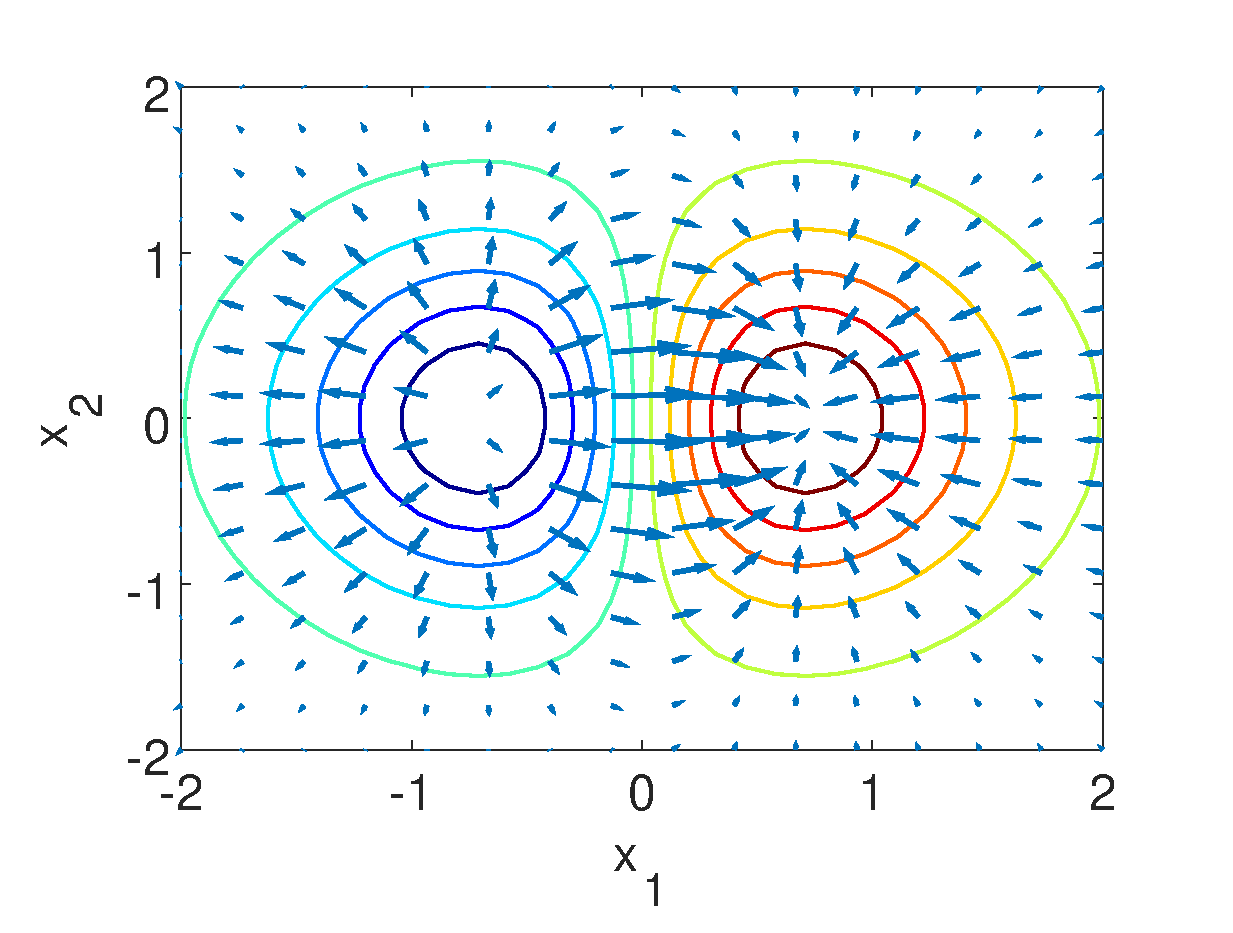
\includegraphics[width=\textwidth]{chapters/derivada/mfiles/gradiente/gradient.eps}
        \caption{Gráfico de $e(\VECTOR{x})$ como curvas de nível e $\triangledown e(\VECTOR{x})$ como vetores.}
        \label{fig:ex:gradient}
    \end{figure}
\end{minipage}

%%%%%%%%%%%%%%%%%%%%%%%%%%%%%%%%%%%%%%%%%%%%%%%%%%%%%%%%%%%%%%%%%%%%%%%%%%%%%%%%
\index{Matriz Jacobiana}
\begin{proposition}[Matriz Jacobiana de $\VECTOR{f}(\VECTOR{x})$:]\label{def:jacobian}
 Dado um vetor coluna, como função $\VECTOR{f}:\mathbb{R}^{N}\rightarrow \mathbb{R}^{M}$ com variável $\VECTOR{x} \in \mathbb{R}^{N}$
 como vetor coluna com elementos $x_n\in \mathbb{R}$ de modo que $n\in \mathbb{N}$, $1 \leq n \leq N$,
 diferenciável em $\VECTOR{x}$. 
 $\MATRIX{J}(\VECTOR{x})$ é chamada matriz Jacobiana \cite[pp. 130]{zhang2017matrix} \cite{Jacobian}  de 
 $\VECTOR{f}(\VECTOR{x})=[f_1(\VECTOR{x})~f_2(\VECTOR{x})~\dots~f_m(\VECTOR{x})~\dots f_M(\VECTOR{x})]^{\transpose}$, de modo que: 
 \begin{equation}
   \frac{\partial \VECTOR{f}(\VECTOR{x})}{\partial \VECTOR{x}^{\transpose} }=
\left[
\begin{matrix}
\frac{\partial \VECTOR{f}(\VECTOR{x}) }{\partial x_{1}}&
\frac{\partial \VECTOR{f}(\VECTOR{x}) }{\partial x_{2}}&
\hdots&
\frac{\partial \VECTOR{f}(\VECTOR{x}) }{\partial x_{n}}&
\hdots&
\frac{\partial \VECTOR{f}(\VECTOR{x}) }{\partial x_{N}}
\end{matrix}
\right]
 \end{equation}

\begin{equation}
\MATRIX{J}(\VECTOR{x})\equiv
\left[\overrightarrow{\triangledown} \VECTOR{f}^{\transpose}(\VECTOR{x})\right]^{\transpose} \equiv 
\frac{\partial \VECTOR{f}(\VECTOR{x})}{\partial \VECTOR{x}^{\transpose} }
\end{equation}

  \begin{equation}
  \MATRIX{J}(\VECTOR{x})\equiv 
\left[
\begin{matrix}
\frac{\partial f_1(\VECTOR{x}) }{\partial x_{1}}&
\frac{\partial f_1(\VECTOR{x}) }{\partial x_{2}}&
\hdots&
\frac{\partial f_1(\VECTOR{x}) }{\partial x_{n}}&
\hdots&
\frac{\partial f_1(\VECTOR{x}) }{\partial x_{N}}\\
\frac{\partial f_2(\VECTOR{x}) }{\partial x_{1}}&
\frac{\partial f_2(\VECTOR{x}) }{\partial x_{2}}&
\hdots&
\frac{\partial f_2(\VECTOR{x}) }{\partial x_{n}}&
\hdots&
\frac{\partial f_2(\VECTOR{x}) }{\partial x_{N}}\\
\vdots&
\vdots&
\hdots&
\vdots&
\vdots&
\vdots\\
\frac{\partial f_m(\VECTOR{x}) }{\partial x_{1}}&
\frac{\partial f_m(\VECTOR{x}) }{\partial x_{2}}&
\hdots&
\frac{\partial f_m(\VECTOR{x}) }{\partial x_{n}}&
\hdots&
\frac{\partial f_m(\VECTOR{x}) }{\partial x_{N}}\\
\vdots&
\vdots&
\hdots&
\vdots&
\vdots&
\vdots\\
\frac{\partial f_M(\VECTOR{x}) }{\partial x_{1}}&
\frac{\partial f_M(\VECTOR{x}) }{\partial x_{2}}&
\hdots&
\frac{\partial f_M(\VECTOR{x}) }{\partial x_{n}}&
\hdots&
\frac{\partial f_M(\VECTOR{x}) }{\partial x_{N}}\\
\end{matrix}
\right]
 \end{equation}
\end{proposition}


\begin{example}[Uso da Proposição \ref{def:jacobian}:]
Conhecida a função $\VECTOR{f}: \mathbb{R}^2 \rightarrow \mathbb{R}^2$,
onde $\VECTOR{u}=\VECTOR{f}(\VECTOR{x})$, 
\begin{equation}
\VECTOR{f}(\VECTOR{x})=
\begin{bmatrix}
\frac{x_1^3+x_2}{5}\\
\frac{x_2^3+x_1}{5}
\end{bmatrix}
\qquad \rightarrow \qquad
\frac{\partial \VECTOR{f}(\VECTOR{x}) }{\partial \VECTOR{x}^{\transpose}}\equiv
\MATRIX{J}(\VECTOR{x})\equiv
\begin{bmatrix}
\VECTOR{j}_{u_1}(\VECTOR{x})\\
\VECTOR{j}_{u_2}(\VECTOR{x})
\end{bmatrix}\equiv
\begin{bmatrix}
\frac{3 x_1^2}{5} & \frac{1}{5}\\
\frac{1}{5}       & \frac{3 x_2^2}{5}
\end{bmatrix}.
\end{equation}
Se $\VECTOR{\hat{x}}=[1~ 1]^{\transpose}$, usando a função $\VECTOR{f}(\VECTOR{\hat{x}})$ 
podemos calcular que $\VECTOR{\hat{u}}=[0.4~ 0.4]^{\transpose}$;
e usando a função $\MATRIX{J}(\VECTOR{\hat{x}})$ obtemos que $\VECTOR{j}_{u_1}(\VECTOR{\hat{x}})=[0.6~ 0.2]$ e $\VECTOR{j}_{u_2}(\VECTOR{\hat{x}})=[0.2~ 0.6]$.
Um gráfico do uso da matriz jacobiana avaliada em $\MATRIX{J}([1~ 1]^{\transpose})$ pode ser visto na Figura \ref{fig:ex:jacobiano}.
\end{example}

\begin{figure}[!h]
    \centering
    \begin{subfigure}[b]{0.49\textwidth}
        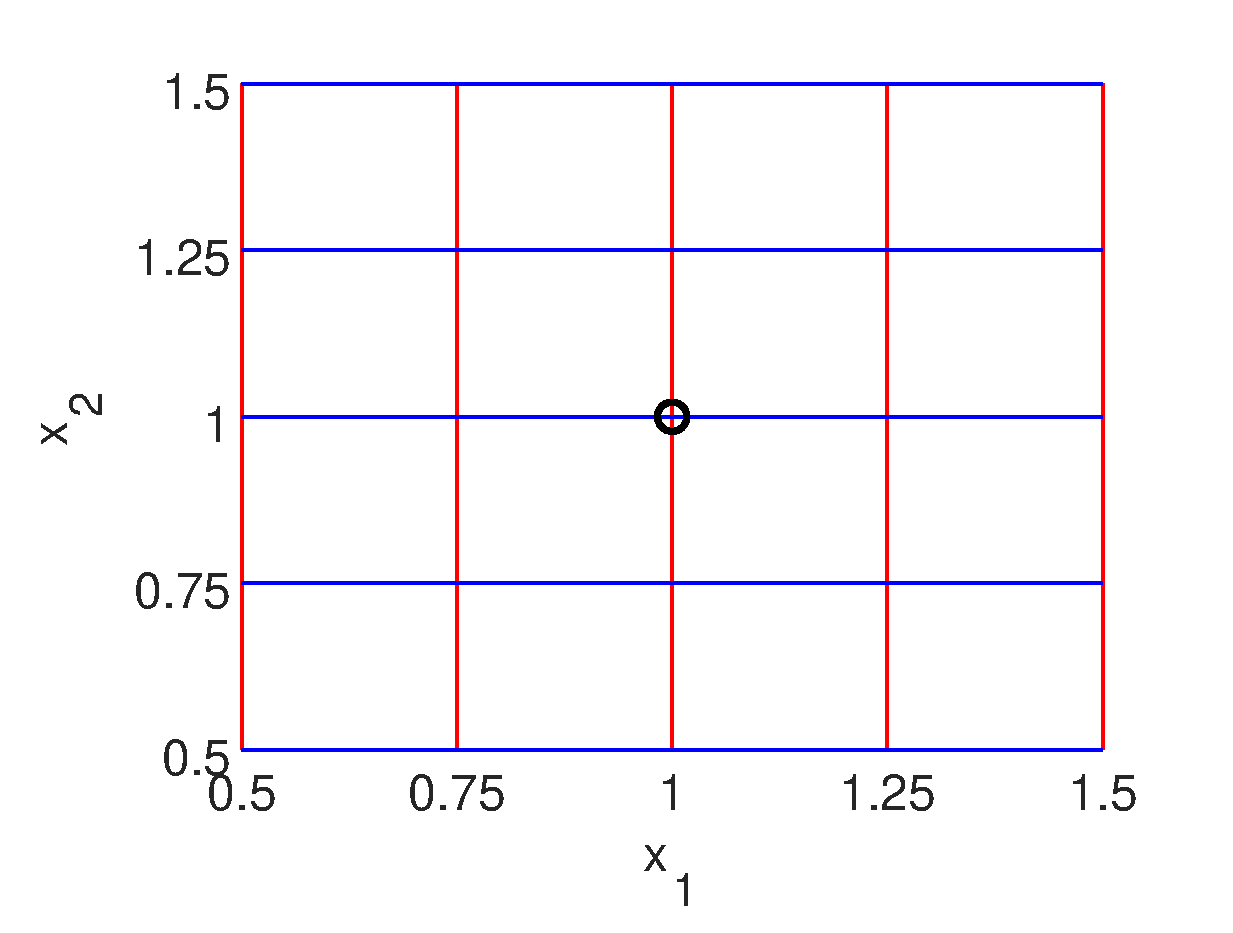
\includegraphics[width=\textwidth]{chapters/derivada/mfiles/jacobian/jacobian1.eps}
        \caption{Gráfico do ponto $\VECTOR{\hat{x}}$ e linhas auxiliares. ~~~~~~~~~ ~~~~~~~~~ ~~~~~~~~~}
        \label{fig:ex:jacobiano:x}
    \end{subfigure}
    ~ %add desired spacing between images, e. g. ~, \quad, \qquad, \hfill etc. 
      %(or a blank line to force the subfigure onto a new line)
    \begin{subfigure}[b]{0.49\textwidth}
        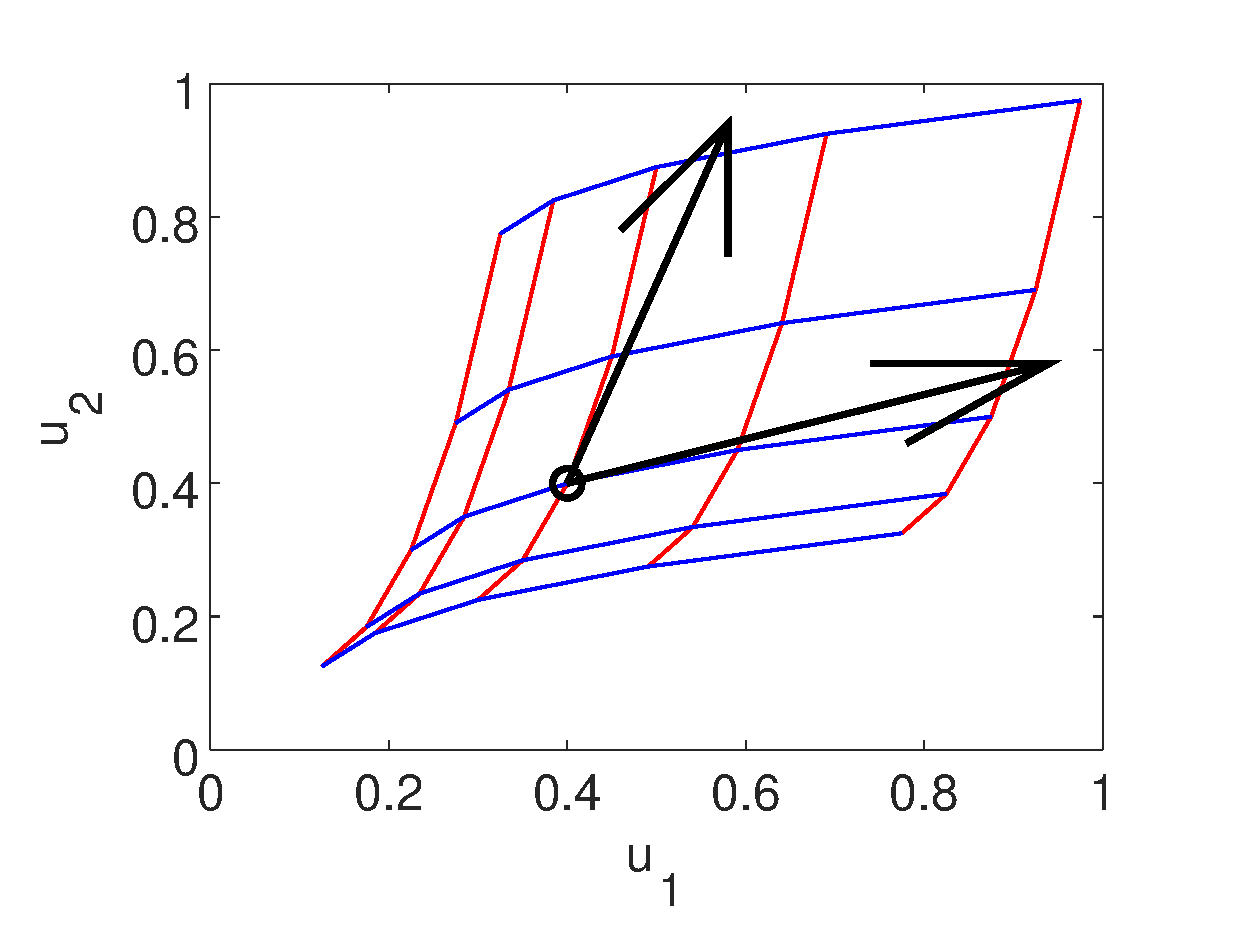
\includegraphics[width=\textwidth]{chapters/derivada/mfiles/jacobian/jacobian2.eps}
        \caption{Gráfico do ponto $\VECTOR{\hat{u}}$, dos vetores $\VECTOR{j}_{u_1}(\VECTOR{\hat{x}})$ e
    $\VECTOR{j}_{u_2}(\VECTOR{\hat{x}})$, e da avaliação das linhas auxiliares na função $\VECTOR{f}$.}
        \label{fig:ex:jacobiano:u}
    \end{subfigure}
    \caption{Gráfico do uso da matriz jacobiana.}
    \label{fig:ex:jacobiano}
\end{figure}


%%%%%%%%%%%%%%%%%%%%%%%%%%%%%%%%%%%%%%%%%%%%%%%%%%%%%%%%%%%%%%%%%%%%%%%%%%%%%%%%
\index{Matriz Hessiana}
\begin{proposition}[$\triangledown^2 e(\VECTOR{x})$ - Matriz Hessiana de $e(\VECTOR{x})$:]\label{def:hessian}
 Dada uma função $e:\mathbb{R}^{N}\rightarrow \mathbb{R}$ com variável $\VECTOR{x} \in \mathbb{R}^{N}$
 como vetor coluna  com elementos $x_n\in \mathbb{R}$ de modo que $n\in \mathbb{N}$, $1 \leq n \leq N$,
 diferenciável em $\VECTOR{x}$. 
 $\MATRIX{H}(\VECTOR{x})$ é chamada matriz Hessiana \cite[pp. 150]{zhang2017matrix} \cite{Hessian} 
 de $e(\VECTOR{x})$, de modo que: 
\begin{equation}
  \MATRIX{H}(\VECTOR{x}) \equiv  \overrightarrow{\triangledown} \overrightarrow{\triangledown}^{\transpose}e(\VECTOR{x}) \equiv  
\triangledown^2 e(\VECTOR{x}) \equiv \frac{\partial }{\partial \VECTOR{x}} \left( \frac{\partial e(\VECTOR{x})}{ \partial \VECTOR{x}^{\transpose} }\right) 
\end{equation}
 \begin{equation}
  \MATRIX{H}(\VECTOR{x}) =
\left[
\begin{matrix}
\frac{\partial^2 e(\VECTOR{x}) }{\partial x_{1}\partial x_{1}}&
\frac{\partial^2 e(\VECTOR{x}) }{\partial x_{1}\partial x_{2}}&
\hdots&
\frac{\partial^2 e(\VECTOR{x}) }{\partial x_{1}\partial x_{n}}&
\hdots&
\frac{\partial^2 e(\VECTOR{x}) }{\partial x_{1}\partial x_{N}}\\
\frac{\partial^2 e(\VECTOR{x}) }{\partial x_{2}\partial x_{1}}&
\frac{\partial^2 e(\VECTOR{x}) }{\partial x_{2}\partial x_{2}}&
\hdots&
\frac{\partial^2 e(\VECTOR{x}) }{\partial x_{2}\partial x_{n}}&
\hdots&
\frac{\partial^2 e(\VECTOR{x}) }{\partial x_{2}\partial x_{N}}\\
\vdots&
\vdots&
\vdots&
\vdots&
\vdots&
\vdots\\
\frac{\partial^2 e(\VECTOR{x}) }{\partial x_{m}\partial x_{1}}&
\frac{\partial^2 e(\VECTOR{x}) }{\partial x_{m}\partial x_{2}}&
\hdots&
\frac{\partial^2 e(\VECTOR{x}) }{\partial x_{m}\partial x_{n}}&
\hdots&
\frac{\partial^2 e(\VECTOR{x}) }{\partial x_{m}\partial x_{N}}\\
\vdots&
\vdots&
\vdots&
\vdots&
\vdots&
\vdots\\
\frac{\partial^2 e(\VECTOR{x}) }{\partial x_{M}\partial x_{1}}&
\frac{\partial^2 e(\VECTOR{x}) }{\partial x_{M}\partial x_{2}}&
\hdots&
\frac{\partial^2 e(\VECTOR{x}) }{\partial x_{M}\partial x_{n}}&
\hdots&
\frac{\partial^2 e(\VECTOR{x}) }{\partial x_{M}\partial x_{N}}\\
\end{matrix}
\right]
 \end{equation}
\end{proposition}



\index{Hesse, Ludwig Otto}
\begin{elaboracion}[title=Ludwig Otto Hesse (1811-1874), width= 0.99\linewidth]
Ele foi um matemático alemão que trabalhou em muitos temas como a matriz de Hessiana, 
o grupo Hessiano, os pares Hessianos, entre outras contribuições \cite[pp. 261]{agarwal2014creators}.
\end{elaboracion}


%%%%%%%%%%%%%%%%%%%%%%%%%%%%%%%%%%%%%%%%%%%%%%%%%%%%%%%%%%%%%%%%%%%%%%%%%%%%%%%%
\newpage

%%%%%%%%%%%%%%%%%%%%%%%%%%%%%%%%%%%%%%%%%%%%%%%%%%%%%%%%%%%%%%%%%%%%%%%%%%%%%%%%%%%%%%%
%%%%%%%%%%%%%%%%%%%%%%%%%%%%%%%%%%%%%%%%%%%%%%%%%%%%%%%%%%%%%%%%%%%%%%%%%%%%%%%%%%%%%%%
%%%%%%%%%%%%%%%%%%%%%%%%%%%%%%%%%%%%%%%%%%%%%%%%%%%%%%%%%%%%%%%%%%%%%%%%%%%%%%%%%%%%%%%
\section{Serie de Taylor de $d(x)$, $e(\VECTOR{x})$ e $\VECTOR{f}(\VECTOR{x})$}
\label{def:taylor}


\index{Serie de Taylor!$d:\mathbb{R} \rightarrow \mathbb{R}$}
\begin{proposition}[Serie de Taylor de $d(x)$:]\label{prop:taylord}
Dada uma função $d:\mathbb{R}\rightarrow \mathbb{R}$ com variável $x \in \mathbb{R}$;
infinitamente diferenciável em $a \in \mathbb{R}$;
esta pode ser expressada mediante uma somatória, em serie de Taylor 
\cite[pp. 764]{stewart2008calculus} \cite[pp. 281]{telles2015matematica} \cite{Taylor} 
ao redor de $a$, como
mostra a Eq. (\ref{eq:taylord1}),% onde $\left.\frac{\partial^k d(x)}{\partial x^k}\right|_{x=a}\equiv d^{(k)}(a) $.
\begin{equation}\label{eq:taylord0a}
\left.\frac{\partial^k d(x)}{\partial x^k}\right|_{x=a}\equiv d^{(k)}(a) 
\end{equation}
\begin{equation}\label{eq:taylord1}
  d(x)=d(a)
      ~+\frac{d'(a)}{1!} (x-a)
      ~+\frac{d''(a)}{2!} (x-a)^{2}
      ~+\cdots 
      ~+\frac{d^{(k)}(a)}{k!} (x-a)^{k}
      ~+\cdots 
\end{equation}
A equação pode ser escrita de forma mais compacta mediante uma somatória  como mostra a Eq. (\ref{eq:taylord2}),
\begin{equation}\label{eq:taylord2}
  d(x)=\sum\limits_{k=0}^{+\infty} \frac{d^{(k)}(a)}{k!} (x-a)^{k}.
\end{equation}
\end{proposition}


\begin{example}[Serie de Taylor do $cos(x)$:]
Podem ser vistas aproximações da função $d(x)=cos(x)$, 
mediante o uso da Proposição \ref{prop:taylord} onde é descrita a serie de Taylor ao redor do ponto $a=0$;
aqui é truncada a serie ate a derivada de ordem $4$, $8$ e $10$,
obtendo as aproximações $d_4(x)$, $d_8(x)$ e $d_{10}(x)$,
como pode ser visto na Fig. \ref{fig:taylore}.
\begin{equation}
d^{(k)}(x)=
\left\{
\begin{matrix}
cos(x) & ~if & (k~mod~4)=0\\
-sin(x)& ~if & (k~mod~4)=1\\
-cos(x)& ~if & (k~mod~4)=2\\
sin(x) & ~if & (k~mod~4)=3
\end{matrix}
\right.
\quad \rightarrow \quad
d^{(k)}(0)=
\left\{
\begin{matrix}
1 & ~if & (k~mod~4)=0\\
0& ~if & (k~mod~4)=1\\
-1& ~if & (k~mod~4)=2\\
0 & ~if & (k~mod~4)=3
\end{matrix}
\right.
\end{equation}

\begin{equation}
d_{4}(x)=
1
-\frac{x^{2}}{2!} 
+\frac{x^{4}}{4!},
\qquad 
d_{8}(x)=
1
-\frac{x^{2}}{2!} 
+\frac{x^{4}}{4!} 
-\frac{x^{6}}{6!} 
+\frac{x^{8}}{8!}, 
\end{equation}
\begin{equation}
d_{10}(x)=
1
-\frac{x^{2}}{2!} 
+\frac{x^{4}}{4!} 
-\frac{x^{6}}{6!} 
+\frac{x^{8}}{8!} 
-\frac{x^{10}}{10!} 
\end{equation}
\end{example}

\begin{figure}[!h]
  \centering
    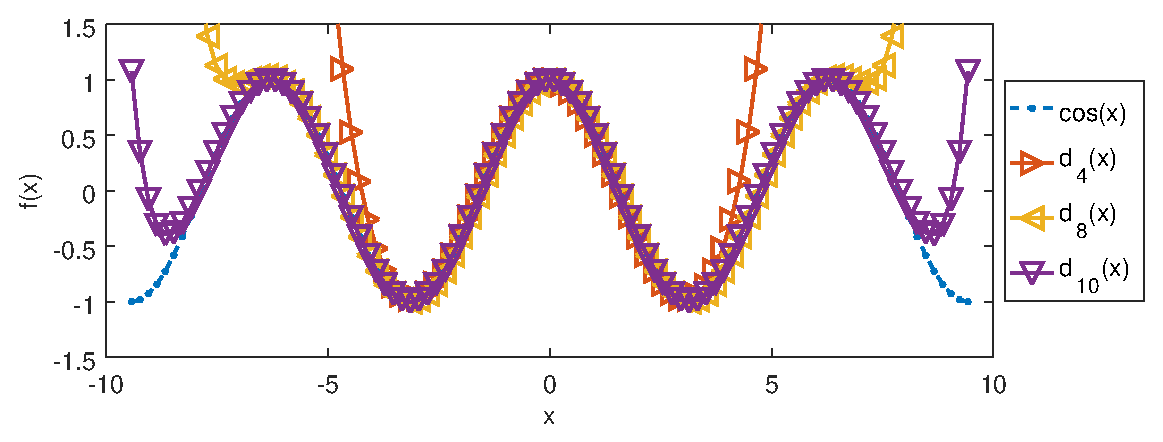
\includegraphics[width=0.90\textwidth]{chapters/funcoes/mcode/taylore.eps}
  \caption{Aproximação da função $cos(x)$ usando a serie de Taylor truncada.}
    \label{fig:taylore}
\end{figure}
 
%%%%%%%%%%%%%%%%%%%%%%%%%%%%%%%%%%%%%%%%%%%%%%%%%%%%%%%%%%%%%%%%%%%%%%%%%%%%%%%%%%%%%%%
 \index{Serie de Taylor!$f:\mathbb{R}^{N}\rightarrow \mathbb{R}$}
\begin{proposition}[Serie de Taylor de $f(\VECTOR{x})$]\label{prop:taylore}
Dada uma função $f:\mathbb{R}^{N}\rightarrow \mathbb{R}$ com variável $\VECTOR{x} \in \mathbb{R}^{N}$, vetor coluna;
infinitamente diferenciável em $\VECTOR{a} \in \mathbb{R}^{N}$;
esta pode ser expressada mediante uma somatória, em serie de Taylor 
\cite[pp. 187, 207]{zhang2017matrix} \cite{Taylor}  ao redor de $\VECTOR{a}$, como
mostra a Eq. (\ref{eq:taylore1}),
\begin{equation}\label{eq:taylore1}
f(\VECTOR{x}) =\sum _{k_{1}=0}^{\infty }\cdots \sum _{k_{N}=0}^{\infty }\left.\left({\frac {\partial ^{k_{1}+\cdots +k_{N}}f(\VECTOR{x})}{\partial x_{1}^{k_{1}}\cdots \partial x_{N}^{k_{N}}}}\right)\right|_{\VECTOR{x}=\VECTOR{a}} {\frac {(x_{1}-a_{1})^{k_{1}}\cdots (x_{N}-a_{N})^{k_{N}}}{k_{1}!\cdots k_{N}!}}
\end{equation}

Outra forma alternativa de expressar a função anterior é usando vetores e matrizes,
como na Eq. (\ref{eq:taylore2}).
\begin{equation}\label{eq:taylore2}
  f(\VECTOR{x})=f(\VECTOR{a})
      ~+ \triangledown f(\VECTOR{a})^{\transpose} (\VECTOR{x}-\VECTOR{a})
      ~+\frac{1}{2!}(\VECTOR{x}-\VECTOR{a})^{\transpose} \MATRIX{H(\VECTOR{a})}  (\VECTOR{x}-\VECTOR{a})
      ~+\cdots 
\end{equation}
Onde o vector $\triangledown f(\VECTOR{x})\equiv \frac{\partial f(\VECTOR{x})}{\partial \VECTOR{x} }$ 
(também chamado \hyperref[def:gradient]{gradiente}),
e a matriz $\MATRIX{H}(\VECTOR{x})\equiv \frac{\partial }{\partial \VECTOR{x}} \left( \frac{\partial f(\VECTOR{x})}{ \partial \VECTOR{x}^{\transpose} }\right)$
(também chamada matriz \hyperref[def:hessian]{Hessiana}).
\end{proposition}

%%%%%%%%%%%%%%%%%%%%%%%%%%%%%%%%%%%%%%%%%%%%%%%%%%%%%%%%%%%%%%%%%%%%%%%%%%%%%%%%%%%%%%%
\index{Serie de Taylor!$\VECTOR{f}:\mathbb{R}^{N}\rightarrow \mathbb{R}^{M}$}
\begin{proposition}[Serie de Taylor de $\VECTOR{f}(\VECTOR{x})$]\label{prop:taylorf}
Dada uma função de contra-domino vectorial $\VECTOR{f}:\mathbb{R}^{N}\rightarrow \mathbb{R}^{M}$, 
sendo $\VECTOR{f}$ um vector coluna, com variável $\VECTOR{x} \in \mathbb{R}^{N}$, vetor coluna;
infinitamente diferenciável em $\VECTOR{a} \in \mathbb{R}^{N}$;
esta pode ser expressada mediante uma somatória, em serie de Taylor 
\cite[pp. 393]{levine1999control} \cite{Taylor} ao redor de $\VECTOR{a}$, como
mostra a Eq. (\ref{eq:taylorf1}),
\begin{equation}\label{eq:taylorf1}
\VECTOR{f}(\VECTOR{x}) =\VECTOR{f}(\VECTOR{a})
      ~+ \MATRIX{J}(\VECTOR{a}) (\VECTOR{x}-\VECTOR{a})
      ~+\cdots 
\end{equation}

Onde a matriz $\MATRIX{J}(\VECTOR{x})\equiv \frac{\partial \VECTOR{f}(\VECTOR{x})}{\partial \VECTOR{x}^{\transpose} }$,
também conhecido como matriz \hyperref[def:jacobian]{Jacobiana} de $\VECTOR{f}(\VECTOR{x})$.
\end{proposition}



\chapterimage{chapter_derivada.pdf} % Chapter heading image

\chapter{Derivada de funções de variável vetorial: $\mathbb{R}^{N}$}

%%%%%%%%%%%%%%%%%%%%%%%%%%%%%%%%%%%%%%%%%%%%%%%%%%%%%%%%%%%%%%%%%%%%%%%%%%%%%%%%

%%%%%%%%%%%%%%%%%%%%%%%%%%%%%%%%%%%%%%%%%%%%%%%%%%%%%%%%%%%%%%%%%%%%%%%%%%%%%%%%%%%%%%%
%%%%%%%%%%%%%%%%%%%%%%%%%%%%%%%%%%%%%%%%%%%%%%%%%%%%%%%%%%%%%%%%%%%%%%%%%%%%%%%%%%%%%%%
\section{Derivada de $\MATRIX{A}\VECTOR{x}$}

\begin{theorem}\label{theo:derAx}
Se 
$\VECTOR{x}\in \mathbb{R}^N$ é um vetor coluna com elementos $x_n$ de modo que
$n\in \mathbb{N}$, $1 \leq n \leq N$, e 
$\MATRIX{A} \in \mathbb{R}^{M\times N}$ é uma matriz com elementos $a_{mn}$ de modo que
$m\in \mathbb{N}$, $1 \leq m \leq M$, 
então se cumpre\footnote{A demostração pode ser vista na Prova \ref{proof:theo:derAx}.} que:
\begin{equation}
\frac{\partial \MATRIX{A}\VECTOR{x}}{\partial x_n}=a_{:n}
\end{equation}
\end{theorem}
~

\begin{corollary}[Derivada de $\MATRIX{A}\VECTOR{x}$ em relação ao vector $\VECTOR{x}^{\transpose}$]\label{coro:derAx1}
Aplicando a Definição \ref{def:deltahor2} junto ao Teorema \ref{theo:derAx}, é
fácil deduzir que:
\begin{equation}
\frac{\partial \MATRIX{A}\VECTOR{x}}{\partial \VECTOR{x}^{\transpose}}=
\MATRIX{A}=
\left[
\begin{matrix}
 a_{:1} &  a_{:2} &  \cdots &  a_{:N}
\end{matrix}
\right]
\end{equation}
\end{corollary}
~

\begin{corollary}[Derivada de $\MATRIX{A}\VECTOR{x}$ em relação ao vector $\VECTOR{x}$]\label{coro:derAx2}
Aplicando a Definição \ref{def:deltaver} junto ao Teorema \ref{theo:derAx}, é
fácil deduzir que:
\begin{equation}
\frac{\partial \MATRIX{A}\VECTOR{x}}{\partial \VECTOR{x}}=\funcvec(\MATRIX{A})=
\left[
\begin{matrix}
 a_{:1} \\  
a_{:2} \\  
\vdots \\  
a_{:n} \\  
\vdots \\  
a_{:N}
\end{matrix}
\right]
\end{equation}
\end{corollary}

\newpage
\begin{corollary}[Derivada de $\VECTOR{a}^{\transpose}\VECTOR{x}$ em relação ao vector $\VECTOR{x}^{\transpose}$]\label{coro:derAx3}
Aplicando a Definição \ref{def:deltahor} junto ao Teorema \ref{theo:derAx} e sabendo que $\VECTOR{a}^{\transpose}$
é um vetor linha, é
fácil deduzir que:
\begin{equation}
\frac{\partial \VECTOR{a}^{\transpose}\VECTOR{x}}{\partial \VECTOR{x}^{\transpose}}=\VECTOR{a}^{\transpose}
\end{equation}
\end{corollary}

\begin{corollary}[Derivada de $\VECTOR{a}^{\transpose}\VECTOR{x}$ em relação ao vector $\VECTOR{x}$]\label{coro:derAx4}
Aplicando a Definição \ref{def:deltaver} junto ao Teorema \ref{theo:derAx} e sabendo que $\VECTOR{a}^{\transpose}$
é um vetor linha, é
fácil deduzir que:
\begin{equation}
\frac{\partial \VECTOR{a}^{\transpose}\VECTOR{x}}{\partial \VECTOR{x}}=\VECTOR{a}
\end{equation}
\end{corollary}

%%%%%%%%%%%%%%%%%%%%%%%%%%%%%%%%%%%%%%%%%%%%%%%%%%%%%%%%%%%%%%%%%%%%%%%%%%%%%%%%

%%%%%%%%%%%%%%%%%%%%%%%%%%%%%%%%%%%%%%%%%%%%%%%%%%%%%%%%%%%%%%%%%%%%%%%%%%%%%%%%%%%%%%%
%%%%%%%%%%%%%%%%%%%%%%%%%%%%%%%%%%%%%%%%%%%%%%%%%%%%%%%%%%%%%%%%%%%%%%%%%%%%%%%%%%%%%%%
\section{Derivada de $||\MATRIX{A}\VECTOR{x}||^2$ 
}

\begin{theorem}\label{theo:derxAtAx}
Se 
$\VECTOR{x}\in \mathbb{R}^N$ é um vetor coluna com elementos $x_n$ de modo que
$n\in \mathbb{N}$, $1 \leq n \leq N$, e 
$\MATRIX{A} \in \mathbb{R}^{M\times N}$ é uma matriz com elementos $a_{mn}$ de modo que
$m\in \mathbb{N}$, $1 \leq m \leq M$, 
então se cumpre\footnote{A demostração pode ser vista na Prova \ref{proof:theo:derxAtAx}.} que:
\begin{equation}
\begin{matrix}
\frac{\partial ||\MATRIX{A}\VECTOR{x}||^2 }{\partial x_n}&=&
\frac{\partial \left(\MATRIX{A}\VECTOR{x}\right)^{\transpose}\left(\MATRIX{A}\VECTOR{x}\right)}{\partial x_n}&=&
2\left(\MATRIX{A}\VECTOR{x}\right)^{\transpose}a_{:n}\\
~&~&~&=& 2\left(a_{:n}\right)^{\transpose}\MATRIX{A}\VECTOR{x}
\end{matrix}
\end{equation}
\end{theorem}

\begin{corollary}[Derivada de $||\MATRIX{A}\VECTOR{x}||^2$ em relação ao vector $\VECTOR{x}^{\transpose}$]\label{coro:derxAtAx1}
Aplicando a Definição \ref{def:deltahor} junto ao Teorema \ref{theo:derxAtAx}, é
fácil deduzir que:
\begin{equation}
\frac{\partial ||\MATRIX{A}\VECTOR{x}||^2 }{\partial \VECTOR{x}^{\transpose}}=
2\left(\MATRIX{A}^{\transpose}\MATRIX{A}\VECTOR{x}\right)^{\transpose}
\end{equation}
%\frac{\partial \left(\MATRIX{A}\VECTOR{x}\right)^{\transpose}\left(\MATRIX{A}\VECTOR{x}\right)}{\partial \VECTOR{x}^{\transpose}}=
\end{corollary}

\begin{corollary}[Derivada de $||\MATRIX{A}\VECTOR{x}||^2$ em relação ao vector $\VECTOR{x}$]\label{coro:derxAtAx2}
Aplicando a Definição \ref{def:deltaver} junto ao Teorema \ref{theo:derxAtAx}, é
fácil deduzir que:
\begin{equation}
\frac{\partial ||\MATRIX{A}\VECTOR{x}||^2 }{\partial \VECTOR{x}}=
2 \MATRIX{A}^{\transpose}\MATRIX{A}\VECTOR{x}
\end{equation}
%\frac{\partial \left(\MATRIX{A}\VECTOR{x}\right)^{\transpose}\left(\MATRIX{A}\VECTOR{x}\right)}{\partial \VECTOR{x}}=
\end{corollary}

%%%%%%%%%%%%%%%%%%%%%%%%%%%%%%%%%%%%%%%%%%%%%%%%%%%%%%%%%%%%%%%%%%%%%%%%%%%%%%%%

%%%%%%%%%%%%%%%%%%%%%%%%%%%%%%%%%%%%%%%%%%%%%%%%%%%%%%%%%%%%%%%%%%%%%%%%%%%%%%%%%%%%%%%
%%%%%%%%%%%%%%%%%%%%%%%%%%%%%%%%%%%%%%%%%%%%%%%%%%%%%%%%%%%%%%%%%%%%%%%%%%%%%%%%%%%%%%%
\section{Derivada de $||\MATRIX{A}\VECTOR{x}-\VECTOR{b}||_{\MATRIX{C}}^2$ 
}

\begin{theorem}\label{theo:derAxbAxb}
Se 
$\VECTOR{x}\in \mathbb{R}^N$ é um vetor coluna com elementos $x_n$, de modo que
$n\in \mathbb{N}$, $1 \leq n \leq N$, 
$\VECTOR{b}\in \mathbb{R}^M$ é um vetor coluna com elementos $b_m$, de modo que
$m\in \mathbb{N}$, $1 \leq m \leq M$,  
$\MATRIX{A} \in \mathbb{R}^{M\times N}$ é uma matriz com elementos $a_{mn}$, e
$\MATRIX{C} \in \mathbb{R}^{M\times M}$ é uma matriz diagonal, 
então se cumpre\footnote{A demonstração pode ser vista na Prova \ref{proof:theo:derAxbAxb}.} que:
\begin{equation}
\begin{matrix}
\frac{\partial ||\MATRIX{A}\VECTOR{x}-\VECTOR{b}||_{\MATRIX{C}}^2}{\partial x_n}&=&
\frac{\partial \left(\MATRIX{A}\VECTOR{x}-\VECTOR{b}\right)^{\transpose}\MATRIX{C}\left(\MATRIX{A}\VECTOR{x}-\VECTOR{b}\right)}{\partial x_n}&=&
2\left(\MATRIX{A}\VECTOR{x}-\VECTOR{b}\right)^{\transpose}\MATRIX{C}a_{:n}\\
~&~&~&=& 2\left(a_{:n}\right)^{\transpose}\MATRIX{C}\left(\MATRIX{A}\VECTOR{x}-  \VECTOR{b}\right)
\end{matrix}
\end{equation}
\end{theorem}

\begin{corollary}[Derivada de 
$||\MATRIX{A}\VECTOR{x}-\VECTOR{b}||_{\MATRIX{C}}^2$ em 
relação ao vetor $\VECTOR{x}^{\transpose}$:]\label{coro:derAxbAxb1}
Aplicando a Definição \ref{def:deltahor} junto ao Teorema \ref{theo:derAxbAxb}, é
fácil deduzir que:
\begin{equation}
\frac{\partial ||\MATRIX{A}\VECTOR{x}-\VECTOR{b}||_{\MATRIX{C}}^2}{\partial \VECTOR{x}^{\transpose}}=
2\left(\MATRIX{A}\VECTOR{x}- \VECTOR{b} \right)^{\transpose}\MATRIX{C}\MATRIX{A}
\end{equation}
\end{corollary}

\begin{corollary}[Derivada de 
$||\MATRIX{A}\VECTOR{x}-\VECTOR{b}||_{\MATRIX{C}}^2$ em 
relação ao vetor $\VECTOR{x}$:]\label{coro:derAxbAxb2}
Aplicando a Definição \ref{def:deltaver} junto ao Teorema \ref{theo:derAxbAxb}, é
fácil deduzir que:
\begin{equation}
\frac{\partial ||\MATRIX{A}\VECTOR{x}-\VECTOR{b}||_{\MATRIX{C}}^2}{\partial \VECTOR{x} }=
2 \MATRIX{A}^{\transpose}\MATRIX{C}\left(\MATRIX{A}\VECTOR{x}-\VECTOR{b}\right)
\end{equation}
\end{corollary}

%%%%%%%%%%%%%%%%%%%%%%%%%%%%%%%%%%%%%%%%%%%%%%%%%%%%%%%%%%%%%%%%%%%%%%%%%%%%%%%%

%%%%%%%%%%%%%%%%%%%%%%%%%%%%%%%%%%%%%%%%%%%%%%%%%%%%%%%%%%%%%%%%%%%%%%%%%%%%%%%%%%%%%%%
%%%%%%%%%%%%%%%%%%%%%%%%%%%%%%%%%%%%%%%%%%%%%%%%%%%%%%%%%%%%%%%%%%%%%%%%%%%%%%%%%%%%%%%
\section{Derivada de $||\VECTOR{f}(\VECTOR{x})-\VECTOR{b}||_{\MATRIX{C}}^2$  
}

\begin{theorem}[Valor exato:]\label{theo:derfxbCfxb0}
Se 
$\VECTOR{x}\in \mathbb{R}^N$ e, 
$\VECTOR{b}\in \mathbb{R}^M$ são vetores coluna,  
$\VECTOR{f}: \mathbb{R}^{N}\rightarrow \mathbb{R}^{M}$ é uma função vetorial de valor vectorial, e
$\MATRIX{C} \in \mathbb{R}^{M\times M}$ é uma matriz diagonal, 
então se cumpre\footnote{A demostração pode ser vista na Prova \ref{proof:theo:derfxbCfxb0}.} a Eq. (\ref{eq:theo:derfxbCfxb0}),
onde $\MATRIX{J}(\VECTOR{x})$ é a \hyperref[def:jacobian]{\textbf{matriz Jacobiana}} de $\VECTOR{f}(\VECTOR{x})$,
\begin{equation}\label{eq:theo:derfxbCfxb0}
\frac{\partial ||\VECTOR{f}(\VECTOR{x})-\VECTOR{b}||_{\MATRIX{C}}^2}{\partial \VECTOR{x}} =
2 \MATRIX{J}(\VECTOR{x})^{\transpose}\MATRIX{C}\left[\VECTOR{f}(\VECTOR{x})-\VECTOR{b}\right].
\end{equation}

\end{theorem}

\begin{theorem}[Valor aproximado:]\label{theo:derfxbCfxb}
Se 
$\VECTOR{x}\in \mathbb{R}^N$ é um vetor coluna, 
$\VECTOR{b}\in \mathbb{R}^M$ é um vetor coluna,  
$\VECTOR{f}: \mathbb{R}^{N}\rightarrow \mathbb{R}^{M}$ é uma função vetorial de valor vectorial, e
$\MATRIX{C} \in \mathbb{R}^{M\times M}$ é uma matriz diagonal, 
então se cumpre\footnote{A demostração pode ser vista na Prova \ref{proof:theo:derfxbCfxb}.} que:
\begin{equation}
\frac{\partial ||\VECTOR{f}(\VECTOR{x})-\VECTOR{b}||_{\MATRIX{C}}^2}{\partial \VECTOR{x}} \approx
2 \MATRIX{J}(\VECTOR{p})^{\transpose}\MATRIX{C}\left[\MATRIX{J}(\VECTOR{p})\left(\VECTOR{x} - 
\VECTOR{p}\right)-\left(\VECTOR{b}-\VECTOR{f}(\VECTOR{p})\right)\right].
\end{equation}

Sendo $\VECTOR{p}$ um ponto fixo no domínio de $\VECTOR{f}(\VECTOR{x})$,  ao redor do qual é feita  aproximação
usando a \hyperref[def:taylor]{\textbf{série de Taylor}}, 
$\VECTOR{f}(\VECTOR{x})\approx \VECTOR{f}(\VECTOR{p})+\MATRIX{J}(\VECTOR{p})\left(\VECTOR{x}-\VECTOR{p}\right)$,
onde $\MATRIX{J}(\VECTOR{p})$ é a matriz \hyperref[def:jacobian]{Jacobiana} de $\VECTOR{f}(\VECTOR{x})$ avaliada em $\VECTOR{p}$.

\end{theorem}



%%%%%%%%%%%%%%%%%%%%%%%%%%%%%%%%%%%%%%%%%%%%%%%%%%%%%%%%%%%%%%%%%%%%%%%%%%%%%%%%

%%%%%%%%%%%%%%%%%%%%%%%%%%%%%%%%%%%%%%%%%%%%%%%%%%%%%%%%%%%%%%%%%%%%%%%%%%%%%%%%%%%%%%%
%%%%%%%%%%%%%%%%%%%%%%%%%%%%%%%%%%%%%%%%%%%%%%%%%%%%%%%%%%%%%%%%%%%%%%%%%%%%%%%%%%%%%%%
\section{Derivada de $||\VECTOR{f}(\VECTOR{x})-\VECTOR{b}||_{\MATRIX{C}}^2+\alpha||\VECTOR{x}-\VECTOR{q}||_{\MATRIX{D}}^2$ 
}

\begin{theorem}[Valor exato:]\label{theo:exact:derfxbCfxbxqDxq}
Se 
$\VECTOR{x}\in \mathbb{R}^N$,
$\VECTOR{q}\in \mathbb{R}^N$ e, 
$\VECTOR{b}\in \mathbb{R}^M$ são vetores coluna,  
$\VECTOR{f}: \mathbb{R}^{N}\rightarrow \mathbb{R}^{M}$ é uma função de valor vectorial, e
$\MATRIX{C} \in \mathbb{R}^{M\times M}$ e $\MATRIX{D} \in \mathbb{R}^{N\times N}$ são matrizes diagonais, 
então se cumpre\footnote{A 
demostração pode ser vista na união da Prova \ref{proof:theo:derfxbCfxb0} e o Corolário \ref{coro:derAxbAxb2}.} a Eq. (\ref{eq:theo:exact:derfxbCfxbxqDxq}),
onde $\MATRIX{J}(\VECTOR{x})$ é a \hyperref[def:jacobian]{\textbf{matriz Jacobiana}} de $\VECTOR{f}(\VECTOR{x})$.
\begin{equation}\label{eq:theo:exact:derfxbCfxbxqDxq}
\frac{\partial ||\VECTOR{f}(\VECTOR{x})-\VECTOR{b}||_{\MATRIX{C}}^2+\alpha||\VECTOR{x}-\VECTOR{q}||_{\MATRIX{D}}^2}{\partial \VECTOR{x}} 
= 2 \MATRIX{J}(\VECTOR{x})^{\transpose}\MATRIX{C}\left[\VECTOR{f}(\VECTOR{x})-\VECTOR{b}\right]
+ 2 \alpha\MATRIX{D}\left(\VECTOR{x}-\VECTOR{q}\right),
\end{equation}

\end{theorem}



\begin{theorem}[Valor aproximado:]\label{theo:derfxbCfxbxqDxq}
Se 
$\VECTOR{x}\in \mathbb{R}^N$ é um vetor coluna, 
$\VECTOR{b}\in \mathbb{R}^M$ é um vetor coluna,
$\VECTOR{q}\in \mathbb{R}^N$ é um vetor coluna, 
$\VECTOR{f}: \mathbb{R}^{N}\rightarrow \mathbb{R}^{M}$ é uma função de valor vectorial, 
$\MATRIX{C} \in \mathbb{R}^{M\times M}$ é uma matriz diagonal, e
$\MATRIX{D} \in \mathbb{R}^{N\times N}$ é uma matriz diagonal, 
então se cumpre\footnote{A demostração pode ser vista na Prova \ref{proof:theo:derfxbCfxbxqDxq}.} que:
\begin{equation}
\frac{\partial \left(||\VECTOR{f}(\VECTOR{x})-\VECTOR{b}||_{\MATRIX{C}}^2+\alpha||\VECTOR{x}-\VECTOR{q}||_{\MATRIX{D}}^2\right)}{\partial \VECTOR{x}} \approx
2 \MATRIX{J}(\VECTOR{p})^{\transpose}\MATRIX{C}\left\{\MATRIX{J}(\VECTOR{p})\left[\VECTOR{x} - \VECTOR{p}\right]-\left[\VECTOR{b}-\VECTOR{f}(\VECTOR{p})\right] \right\}
+2\alpha\MATRIX{D}\left[\VECTOR{x}-\VECTOR{q}\right]
\end{equation}

Sendo $\VECTOR{p}$ um ponto fixo no domínio de $\VECTOR{f}(\VECTOR{x})$,  ao redor do qual é feita  aproximação
usando a \hyperref[def:taylor]{\textbf{serie de Taylor}}, 
$\VECTOR{f}(\VECTOR{x})\approx \VECTOR{f}(\VECTOR{p})+\MATRIX{J}(\VECTOR{p})\left(\VECTOR{x}-\VECTOR{p}\right)$,
onde $\MATRIX{J}(\VECTOR{p})$ é a matriz \hyperref[def:jacobian]{Jacobiana} de $\VECTOR{f}(\VECTOR{x})$ avaliada em $\VECTOR{p}$.


\end{theorem}


%%%%%%%%%%%%%%%%%%%%%%%%%%%%%%%%%%%%%%%%%%%%%%%%%%%%%%%%%%%%%%%%%%%%%%%%%%%%%%%%

%%%%%%%%%%%%%%%%%%%%%%%%%%%%%%%%%%%%%%%%%%%%%%%%%%%%%%%%%%%%%%%%%%%%%%%%%%%%%%%%%%%%%%%
%%%%%%%%%%%%%%%%%%%%%%%%%%%%%%%%%%%%%%%%%%%%%%%%%%%%%%%%%%%%%%%%%%%%%%%%%%%%%%%%%%%%%%%
\section{Derivada de segundo ordem de $||\VECTOR{f}(\VECTOR{x})-\VECTOR{b}||_{\MATRIX{C}}^2$ 
}



\begin{theorem}[Valor exato:]\label{theo:der2fxbCfxb0}
Se
$\VECTOR{x}\in \mathbb{R}^N$ e 
$\VECTOR{b}\in \mathbb{R}^M$ são vetores coluna,  
$\VECTOR{f}: \mathbb{R}^{N}\rightarrow \mathbb{R}^{M}$ é uma função de valor vetorial,
$\MATRIX{C} \in \mathbb{R}^{M\times M}$ é uma matriz diagonal, e
definimos a função $e(\VECTOR{x})$ como
\begin{equation}
e(\VECTOR{x})= ||\VECTOR{f}(\VECTOR{x})-\VECTOR{b}||_{\MATRIX{C}}^2;
\end{equation}
então a \hyperref[def:hessian]{\textbf{matriz Hessiana}} $\MATRIX{H}(\VECTOR{x})$ 
de $e(\VECTOR{x})$ é igual\footnote{A demonstração pode ser vista na Prova \ref{proof:theo:der2fxbCfxb0}.} a:
\begin{equation}
\MATRIX{H}(\VECTOR{x}) = \frac{\partial}{\partial \VECTOR{x}^{\transpose}}\left(  
\frac{\partial e(\VECTOR{x}) }{\partial \VECTOR{x}} \right) = 2 \MATRIX{B}(\VECTOR{x})
+2 \MATRIX{J}(\VECTOR{x})^{\transpose}\MATRIX{C} \MATRIX{J}(\VECTOR{x}),
\end{equation}
em que 
\begin{equation}
 \MATRIX{B}(\VECTOR{x})=
{\bigcup\limits_{n=1}^{ \rightarrow }}^{N}\left\{ \frac{\partial \MATRIX{J}(\VECTOR{x})^{\transpose} }{\partial x_{n}} \MATRIX{C} \left( \VECTOR{f}(\VECTOR{x})-\VECTOR{b}\right) \right\},
\end{equation}
e $\MATRIX{J}(\VECTOR{x})$ é a \hyperref[def:jacobian]{\textbf{matriz Jacobiana}} de $\VECTOR{f}(\VECTOR{x})$.
\end{theorem}

\begin{theorem}[Valor aproximado:]\label{theo:der2fxbCfxb0aprox}
Se 
$\VECTOR{x}\in \mathbb{R}^N$ é  
$\VECTOR{b}\in \mathbb{R}^M$ são vetores coluna,  
$\VECTOR{f}: \mathbb{R}^{N}\rightarrow \mathbb{R}^{M}$ é uma função de valor vetorial,
$\MATRIX{C} \in \mathbb{R}^{M\times M}$ é uma matriz diagonal, e 
definimos a função $e(\VECTOR{x})$ como
\begin{equation}
e(\VECTOR{x})= ||\VECTOR{f}(\VECTOR{x})-\VECTOR{b}||_{\MATRIX{C}}^2.
\end{equation}
Então, para achar uma forma aproximada da \hyperref[def:hessian]{\textbf{matriz Hessiana}} $\MATRIX{H}(\VECTOR{x})$ de $e(\VECTOR{x})$, 
podemos usar a aproximação linear de 
$\VECTOR{f}(\VECTOR{x})\approx \VECTOR{f}(\VECTOR{p}) + \MATRIX{J}(\VECTOR{p})$ $\left(\VECTOR{x}-\VECTOR{p}\right)$, 
por meio da \hyperref[def:taylor]{\textbf{série de Taylor}} 
para funções multivariáveis,
em que $\VECTOR{p}$ é um ponto fixo no domínio de $\VECTOR{f}(\VECTOR{x})$ ao redor do qual é feita  aproximação
da função $\VECTOR{f}(\VECTOR{x})$,
e $\MATRIX{J}(\VECTOR{p})$ é a \hyperref[def:jacobian]{\textbf{matriz Jacobiana}} de $\VECTOR{f}(\VECTOR{x})$ avaliada no ponto $\VECTOR{p}$.

Com essas considerações, obtemos\footnote{A demonstração pode ser vista na Prova \ref{proof:theo:der2fxbCfxb0aprox}.} o seguinte resultado,
\begin{equation}
\MATRIX{H}(\VECTOR{x}) = \frac{\partial}{\partial \VECTOR{x}^{\transpose}}\left(  
\frac{\partial e(\VECTOR{x}) }{\partial \VECTOR{x}} \right) \approx 
2 \MATRIX{J}(\VECTOR{p})^{\transpose}\MATRIX{C} \MATRIX{J}(\VECTOR{p}).
\end{equation}


\end{theorem}

%%%%%%%%%%%%%%%%%%%%%%%%%%%%%%%%%%%%%%%%%%%%%%%%%%%%%%%%%%%%%%%%%%%%%%%%%%%%%%%%
\newpage
\section{Provas dos teoremas}

%%%%%%%%%%%%%%%%%%%%%%%%%%%%%%%%%%%%%%%%%%%%%%%%%%%%%%%%%%%%%%%%%%%%%%%%%%%%%%%%%%%%%%%
%%%%%%%%%%%%%%%%%%%%%%%%%%%%%%%%%%%%%%%%%%%%%%%%%%%%%%%%%%%%%%%%%%%%%%%%%%%%%%%%%%%%%%%
\begin{myproofT}[Relativa ao Teorema \ref{theo:derAx}:]\label{proof:theo:derAx}
Dados
uma matriz $\MATRIX{A}=\left[a_{:1}~ a_{:2}~ \hdots~ a_{:n}~ \hdots~ a_{:N}\right]$ e 
um vetor coluna $\VECTOR{x}=\left[x_{1}~ x_{2}~ \hdots~ x_{n}~ \hdots~ x_{N}\right]^{\transpose}$, 
podemos expressar que:
\begin{equation}
\frac{\partial \MATRIX{A}\VECTOR{x}}{\partial x_n}=
\frac{\partial \MATRIX{A}}{\partial x_n}\VECTOR{x}+\MATRIX{A}\frac{\partial \VECTOR{x}}{\partial x_n}=
\MATRIX{A}\frac{\partial \VECTOR{x}}{\partial x_n}.
\end{equation}
Sabendo que $\frac{\partial \VECTOR{x}}{\partial x_n}$ é igual a um vetor 
com um $1$ na posição $n$ e $0$ em qualquer outra posição, obtemos que
\begin{equation}
\frac{\partial \MATRIX{A}\VECTOR{x}}{\partial x_n}=
\left[a_{:1}~ a_{:2}~ \hdots~ a_{:n}~ \hdots~ a_{:N}\right]\left[
\begin{matrix}
 0\\
 0\\
 \vdots\\
 1\\
 \vdots\\
 0
\end{matrix}
\right]=a_{:n}.
\end{equation}
\end{myproofT}

%%%%%%%%%%%%%%%%%%%%%%%%%%%%%%%%%%%%%%%%%%%%%%%%%%%%%%%%%%%%%%%%%%%%%%%%%%%%%%%%%%%%%%%
%%%%%%%%%%%%%%%%%%%%%%%%%%%%%%%%%%%%%%%%%%%%%%%%%%%%%%%%%%%%%%%%%%%%%%%%%%%%%%%%%%%%%%%
\begin{myproofT}[Relativa ao Teorema \ref{theo:derxAtAx}:]\label{proof:theo:derxAtAx}
Dados
uma matriz $\MATRIX{A}=\left[a_{:1}~ a_{:2}~ \hdots~ a_{:n}~ \hdots~ a_{:N}\right]$ e 
um vetor coluna $\VECTOR{x}=\left[x_{1}~ x_{2}~ \hdots~ x_{n}~ \hdots~ x_{N}\right]^{\transpose}$, 
podemos expressar que:
\begin{equation}\label{eq:proof:derxAtAx1}
\frac{\partial ||\MATRIX{A}\VECTOR{x}||^{2}}{\partial x_n}=
\frac{\partial \left(\MATRIX{A}\VECTOR{x}\right)^{\transpose}\left(\MATRIX{A}\VECTOR{x}\right)}{\partial x_n}=
\left(\frac{\partial \MATRIX{A}\VECTOR{x}}{\partial x_n}\right)^{\transpose}\left(\MATRIX{A}\VECTOR{x}\right)+
\left(\MATRIX{A}\VECTOR{x}\right)^{\transpose} \frac{\partial \MATRIX{A}\VECTOR{x}}{\partial x_n}.
\end{equation}
Pelo visto no Teorema \ref{theo:derAx}, podemos substituir valores na Eq. (\ref{eq:proof:derxAtAx1})
e obter:
\begin{equation}\label{eq:proof:derxAtAx2}
\frac{\partial ||\MATRIX{A}\VECTOR{x}||^{2}}{\partial x_n}=
\left(a_{:n}\right)^{\transpose} \MATRIX{A}\VECTOR{x} +
\left(\MATRIX{A}\VECTOR{x}\right)^{\transpose} a_{:n}.
\end{equation}
Como cada um dos somandos da equação anterior é um escalar, podemos aplicar o operador
transposta ($\transpose$) sobre qualquer somando sem alterar o resultado; 
de modo que temos duas possíveis
formas de expressar a solução:
\begin{equation}
\begin{matrix}
\frac{\partial ||\MATRIX{A}\VECTOR{x}||^2 }{\partial x_n}&=&
2\left(\MATRIX{A}\VECTOR{x}\right)^{\transpose}a_{:n}\\
~&=& 2\left(a_{:n}\right)^{\transpose}\MATRIX{A}\VECTOR{x}.
\end{matrix}
\end{equation}
\end{myproofT}

%%%%%%%%%%%%%%%%%%%%%%%%%%%%%%%%%%%%%%%%%%%%%%%%%%%%%%%%%%%%%%%%%%%%%%%%%%%%%%%%%%%%%%%
%%%%%%%%%%%%%%%%%%%%%%%%%%%%%%%%%%%%%%%%%%%%%%%%%%%%%%%%%%%%%%%%%%%%%%%%%%%%%%%%%%%%%%%
\begin{myproofT}[Relativa ao Teorema \ref{theo:derAxbAxb}:]\label{proof:theo:derAxbAxb}
Dados
uma matriz $\MATRIX{A}=\left[a_{:1}~ a_{:2}~ \hdots~ a_{:n}~ \hdots~ a_{:N}\right]$, 
uma matriz diagonal $\MATRIX{C}\in \mathbb{R}^{M\times M}$, 
um vetor coluna $\VECTOR{x}=\left[x_{1}~ x_{2}~ \hdots~ x_{n}~ \hdots~ x_{N}\right]^{\transpose}$, e 
um vetor coluna $\VECTOR{b}\in \mathbb{R}^{M}$, 
podemos expressar que:
\begin{equation}\label{eq:proof:derAxbAxb1}
\frac{\partial ||\MATRIX{A}\VECTOR{x}-\VECTOR{b}||_{\MATRIX{C}}^2}{\partial x_n} =
\frac{\partial \left(\MATRIX{A}\VECTOR{x}-\VECTOR{b}\right)^{\transpose}\MATRIX{C}\left(\MATRIX{A}\VECTOR{x}-\VECTOR{b}\right)}{\partial x_n}=
 \left(\frac{\partial\MATRIX{A}\VECTOR{x}}{\partial x_n}\right)^{\transpose}\MATRIX{C}\left(\MATRIX{A}\VECTOR{x}-\VECTOR{b}\right)+
 \left(\MATRIX{A}\VECTOR{x}-\VECTOR{b}\right)^{\transpose}\MATRIX{C}\left(\frac{\partial\MATRIX{A}\VECTOR{x}}{\partial x_n}\right).
\end{equation}
Pelo visto no Teorema \ref{theo:derAx}, podemos substituir valores na Eq. (\ref{eq:proof:derAxbAxb1})
e obter:
\begin{equation}\label{eq:proof:derAxbAxb2}
\frac{\partial ||\MATRIX{A}\VECTOR{x}-\VECTOR{b}||_{\MATRIX{C}}^{2}}{\partial x_n}=
\left(a_{:n}\right)^{\transpose}\MATRIX{C}\left( \MATRIX{A}\VECTOR{x}-\VECTOR{b}\right) +
\left(\MATRIX{A}\VECTOR{x}-\VECTOR{b}\right)^{\transpose}\MATRIX{C} a_{:n}.
\end{equation}
Como cada um dos somandos da equação anterior é um escalar, podemos aplicar o operador
transposta ($\transpose$) sobre qualquer somando sem alterar o resultado; de modo que temos duas possíveis
forma de expressar a solução:
\begin{equation}
\begin{matrix}
\frac{\partial ||\MATRIX{A}\VECTOR{x}-\VECTOR{b}||_{\MATRIX{C}}^2 }{\partial x_n}&=&
2\left(\MATRIX{A}\VECTOR{x}-\VECTOR{b}\right)^{\transpose}\MATRIX{C}a_{:n}\\
~&=& 2\left(a_{:n}\right)^{\transpose}\MATRIX{C}\left(\MATRIX{A}\VECTOR{x}-\VECTOR{b}\right).
\end{matrix}
\end{equation}
\end{myproofT}

%%%%%%%%%%%%%%%%%%%%%%%%%%%%%%%%%%%%%%%%%%%%%%%%%%%%%%%%%%%%%%%%%%%%%%%%%%%%%%%%%%%%%%%
%%%%%%%%%%%%%%%%%%%%%%%%%%%%%%%%%%%%%%%%%%%%%%%%%%%%%%%%%%%%%%%%%%%%%%%%%%%%%%%%%%%%%%%
\begin{myproofT}[Relativa ao Teorema \ref{theo:derfxbCfxb0}:]\label{proof:theo:derfxbCfxb0}
Dados
uma função $\VECTOR{f}:\mathbb{R}^{N} \rightarrow \mathbb{R}^{M}$, 
uma matriz diagonal $\MATRIX{C}\in \mathbb{R}^{M\times M}$, 
um vetor coluna $\VECTOR{x}=\left[x_{1}~ x_{2}~ \hdots~ x_{n}~ \hdots~ x_{N}\right]^{\transpose}$, e
um vetor coluna $\VECTOR{b}\in \mathbb{R}^{M}$;
podemos expressar que:
\begin{equation}\label{eq:proof:derfxbCfxb01}
\begin{matrix}
\frac{\partial ||\VECTOR{f}(\VECTOR{x})-\VECTOR{b}||_{\MATRIX{C}}^2}{\partial x_{n}} & = &
\frac{\partial \left( \VECTOR{f}(\VECTOR{x})-\VECTOR{b}\right)^{\transpose} \MATRIX{C} \left( \VECTOR{f}(\VECTOR{x})-\VECTOR{b}\right) }{\partial x_{n}} \\
~ &= &
 \left(  \frac{\partial\VECTOR{f}(\VECTOR{x})  }{\partial x_{n}} \right)^{\transpose} \MATRIX{C} \left( \VECTOR{f}(\VECTOR{x})-\VECTOR{b}\right) +
 \left( \VECTOR{f}(\VECTOR{x})-\VECTOR{b}\right)^{\transpose} \MATRIX{C}  \left(  \frac{\partial\VECTOR{f}(\VECTOR{x})  }{\partial x_{n}} \right)\\
~ &= &
 2 \left(  \frac{\partial\VECTOR{f}(\VECTOR{x})  }{\partial x_{n}} \right)^{\transpose} \MATRIX{C} \left( \VECTOR{f}(\VECTOR{x})-\VECTOR{b}\right).
\end{matrix}
\end{equation}
Assim, usando a Definição \ref{def:deltaver} junto com a Eq. (\ref{eq:proof:derfxbCfxb01}),
obtemos:
\begin{equation}\label{eq:proof:derfxbCfxb02}
\frac{\partial ||\VECTOR{f}(\VECTOR{x})-\VECTOR{b}||_{\MATRIX{C}}^2}{\partial \VECTOR{x}}  = 
2 \MATRIX{J}(\VECTOR{x})^{\transpose} \MATRIX{C} \left( \VECTOR{f}(\VECTOR{x})-\VECTOR{b}\right).
\end{equation}
\end{myproofT}


\begin{myproofT}[Relativa ao Teorema \ref{theo:derfxbCfxb}:]\label{proof:theo:derfxbCfxb}
Dados
uma função $\VECTOR{f}:\mathbb{R}^{N} \rightarrow \mathbb{R}^{M}$, 
uma matriz diagonal $\MATRIX{C}\in \mathbb{R}^{M\times M}$, 
um vetor coluna $\VECTOR{x}\in \mathbb{R}^{N}$, 
um vetor coluna $\VECTOR{b}\in \mathbb{R}^{M}$, 
e considerando a aproximação
$\VECTOR{f}(\VECTOR{x})\approx \VECTOR{f}(\VECTOR{p})+\MATRIX{J}(\VECTOR{p})\left(\VECTOR{x}-\VECTOR{p}\right)$,
obtida a partir da \hyperref[def:taylor]{\textbf{série de Taylor}} para funções multivariáveis;
podemos expressar que:
\begin{equation}\label{eq:proof:derfxbCfxb1}
\frac{\partial ||\VECTOR{f}(\VECTOR{x})-\VECTOR{b}||_{\MATRIX{C}}^2}{\partial \VECTOR{x}} \approx
\frac{\partial ||\MATRIX{J}(\VECTOR{p})\VECTOR{x}-\left[\MATRIX{J}(\VECTOR{p})\VECTOR{p}+\VECTOR{b}-\VECTOR{f}(\VECTOR{p})\right]||_{\MATRIX{C}}^2}{\partial \VECTOR{x}}.
\end{equation}
Pelo visto no Corolário \ref{coro:derAxbAxb2}, podemos substituir os valores,
$\MATRIX{J}(\VECTOR{p})$ e 
$\left[\MATRIX{J}(\VECTOR{p})\VECTOR{p}+\VECTOR{b}-\VECTOR{f}(\VECTOR{p})\right]$,
da Eq. (\ref{eq:proof:derfxbCfxb1}), nas variáveis $\MATRIX{A}$ e $\VECTOR{b}$ 
do Corolário \ref{coro:derAxbAxb2}, respectivamente. Assim obtemos:
\begin{equation}\label{eq:proof:derfxbCfxb2}
\frac{\partial ||\MATRIX{J}(\VECTOR{p})\VECTOR{x}-\left[\MATRIX{J}(\VECTOR{p})\VECTOR{p}+\VECTOR{b}-\VECTOR{f}(\VECTOR{p})\right]||_{\MATRIX{C}}^2}{\partial \VECTOR{x}}  = 
2 \MATRIX{J}(\VECTOR{p})^{\transpose}\MATRIX{C}\left( \MATRIX{J}(\VECTOR{p})\VECTOR{x}-\MATRIX{J}(\VECTOR{p})\VECTOR{p}-\VECTOR{b}+\VECTOR{f}(\VECTOR{p})\right).
\end{equation}
\end{myproofT}


%%%%%%%%%%%%%%%%%%%%%%%%%%%%%%%%%%%%%%%%%%%%%%%%%%%%%%%%%%%%%%%%%%%%%%%%%%%%%%%%%%%%%%%
%%%%%%%%%%%%%%%%%%%%%%%%%%%%%%%%%%%%%%%%%%%%%%%%%%%%%%%%%%%%%%%%%%%%%%%%%%%%%%%%%%%%%%%
\begin{myproofT}[Relativa ao Teorema \ref{theo:der2fxbCfxb0}:]\label{proof:theo:der2fxbCfxb0}
Dados
uma função $\VECTOR{f}:\mathbb{R}^{N} \rightarrow \mathbb{R}^{M}$, 
uma matriz diagonal $\MATRIX{C}\in \mathbb{R}^{M\times M}$, 
um vetor coluna $\VECTOR{x}=\left[x_{1}~ x_{2}~ \hdots~ x_{n}~ \hdots~ x_{N}\right]^{\transpose}$, e
um vetor coluna $\VECTOR{b}\in \mathbb{R}^{M}$;
podemos expressar que:
\begin{equation}\label{eq:proof:der2fxbCfxb01}
\begin{matrix}
\frac{\partial }{\partial x_{n}}\left( \frac{\partial ||\VECTOR{f}(\VECTOR{x})-\VECTOR{b}||_{\MATRIX{C}}^2}{\partial \VECTOR{x}} \right) & = &
\frac{\partial 2 \MATRIX{J}(\VECTOR{x})^{\transpose} \MATRIX{C} \left( \VECTOR{f}(\VECTOR{x})-\VECTOR{b}\right)}{\partial x_{n}} \\
~ & = & 2 \frac{\partial \MATRIX{J}(\VECTOR{x})^{\transpose} }{\partial x_{n}} \MATRIX{C} \left( \VECTOR{f}(\VECTOR{x})-\VECTOR{b}\right)+
2  \MATRIX{J}(\VECTOR{x})^{\transpose}  \MATRIX{C} \frac{\partial \left( \VECTOR{f}(\VECTOR{x})-\VECTOR{b}\right) }{\partial x_{n}}\\
~ & = & 2 \frac{\partial \MATRIX{J}(\VECTOR{x})^{\transpose} }{\partial x_{n}} \MATRIX{C} \left( \VECTOR{f}(\VECTOR{x})-\VECTOR{b}\right)+
2  \MATRIX{J}(\VECTOR{x})^{\transpose}  \MATRIX{C} \frac{\partial \VECTOR{f}(\VECTOR{x}) }{\partial x_{n}}.\\
\end{matrix}
\end{equation}
Assim, usando a Definição \ref{def:deltahor} junto com a Eq. (\ref{eq:proof:der2fxbCfxb01}),
obtemos:
\begin{equation}\label{eq:proof:der2fxbCfxb02}
\frac{\partial }{\partial \VECTOR{x}^{\transpose}}\left( \frac{\partial ||\VECTOR{f}(\VECTOR{x})-\VECTOR{b}||_{\MATRIX{C}}^2}{\partial \VECTOR{x}} \right) =
2 {\bigcup\limits_{n=1}^{ \rightarrow }}^{N}\left\{ \frac{\partial \MATRIX{J}(\VECTOR{x})^{\transpose} }{\partial x_{n}} \MATRIX{C} \left( \VECTOR{f}(\VECTOR{x})-\VECTOR{b}\right) \right\} +
2  \MATRIX{J}(\VECTOR{x})^{\transpose}  \MATRIX{C} \frac{\partial \VECTOR{f}(\VECTOR{x}) }{\partial \VECTOR{x}^{\transpose}}.
\end{equation}
\end{myproofT}

\begin{myproofT}[Relativa ao Teorema \ref{theo:der2fxbCfxb0aprox}:]\label{proof:theo:der2fxbCfxb0aprox}
Dados
uma função $\VECTOR{f}:\mathbb{R}^{N} \rightarrow \mathbb{R}^{M}$, 
uma matriz diagonal $\MATRIX{C}\in \mathbb{R}^{M\times M}$, 
os vetores coluna $\VECTOR{x}\in \mathbb{R}^{N}$ e 
$\VECTOR{b}\in \mathbb{R}^{M}$, e
considerando o Toerema \ref{theo:derfxbCfxb} que usa a aproximação
$\VECTOR{f}(\VECTOR{x})\approx \VECTOR{f}(\VECTOR{p}) + \MATRIX{J}(\VECTOR{p})$ $\left(\VECTOR{x}-\VECTOR{p}\right)$,
podemos expressar que:
\begin{equation}\label{eq:proof:der2fxbCfxb01aprox}
\begin{matrix}
\frac{\partial }{\partial \VECTOR{x}^{\transpose}}\left( \frac{\partial ||\VECTOR{f}(\VECTOR{x})-\VECTOR{b}||_{\MATRIX{C}}^2}{\partial \VECTOR{x}} \right) & \approx & 
\frac{\partial 2 \MATRIX{J}(\VECTOR{p})^{\transpose}\MATRIX{C}\left[\MATRIX{J}(\VECTOR{p})\left(\VECTOR{x} - \VECTOR{p}\right)-\left(\VECTOR{b}-\VECTOR{f}(\VECTOR{p})\right)\right]}{\partial \VECTOR{x}^{\transpose}} \\
~ & \approx & \frac{\partial 2 \MATRIX{J}(\VECTOR{p})^{\transpose}\MATRIX{C} \MATRIX{J}(\VECTOR{p})\VECTOR{x}  }{\partial \VECTOR{x}^{\transpose}}
\end{matrix},
\end{equation}
em que $\VECTOR{p}$ é um ponto fixo no domínio de $\VECTOR{f}(\VECTOR{x})$, 
ao redor do qual é feita  aproximação
da função $\VECTOR{f}(\VECTOR{x})$,
e $\MATRIX{J}(\VECTOR{p})$ é a \hyperref[def:jacobian]{\textbf{matriz Jacobiana}} 
de $\VECTOR{f}(\VECTOR{x})$ avaliado no ponto $\VECTOR{p}$.
Assim, usando o Teorema \ref{theo:derAx} na Eq. (\ref{eq:proof:der2fxbCfxb01aprox}),
obtemos,
\begin{equation}\label{eq:proof:der2fxbCfxb01aprox2}
\frac{\partial }{\partial \VECTOR{x}^{\transpose}}\left( \frac{\partial ||\VECTOR{f}(\VECTOR{x})-\VECTOR{b}||_{\MATRIX{C}}^2}{\partial \VECTOR{x}} \right) \approx 
2 \MATRIX{J}(\VECTOR{p})^{\transpose}\MATRIX{C} \MATRIX{J}(\VECTOR{p}).
\end{equation}
\end{myproofT}

%%%%%%%%%%%%%%%%%%%%%%%%%%%%%%%%%%%%%%%%%%%%%%%%%%%%%%%%%%%%%%%%%%%%%%%%%%%%%%%%%%%%%%%
%%%%%%%%%%%%%%%%%%%%%%%%%%%%%%%%%%%%%%%%%%%%%%%%%%%%%%%%%%%%%%%%%%%%%%%%%%%%%%%%%%%%%%%
\begin{myproofT}[Relativa ao Teorema \ref{theo:derfxbCfxbxqDxq}:]\label{proof:theo:derfxbCfxbxqDxq}
Dados
uma função $\VECTOR{f}:\mathbb{R}^{N} \rightarrow \mathbb{R}^{M}$, 
uma matriz diagonal $\MATRIX{C}\in \mathbb{R}^{M\times M}$, 
uma matriz diagonal $\MATRIX{D}\in \mathbb{R}^{N\times N}$, 
um vetor coluna $\VECTOR{x}\in \mathbb{R}^{N}$, 
um vetor coluna $\VECTOR{b}\in \mathbb{R}^{M}$, e 
um vetor coluna $\VECTOR{q}\in \mathbb{R}^{N}$, 
podemos expressar que:
\begin{equation}\label{eq:proof:derfxbCfxbxqDxq1}
\frac{\partial ||\VECTOR{f}(\VECTOR{x})-\VECTOR{b}||_{\MATRIX{C}}^2 +\alpha||\VECTOR{x}-\VECTOR{q}||_{\MATRIX{D}}^2}{\partial \VECTOR{x}} =
\frac{\partial ||\VECTOR{f}(\VECTOR{x})-\VECTOR{b}||_{\MATRIX{C}}^2}{\partial \VECTOR{x}}+
\alpha \frac{\partial ||\VECTOR{x}-\VECTOR{q}||_{\MATRIX{D}}^2}{\partial \VECTOR{x}}.
\end{equation}
Usando o Corolário \ref{coro:derAxbAxb2} na Eq. (\ref{eq:proof:derfxbCfxbxqDxq1}),
obtemos:
\begin{equation}\label{eq:proof:derfxbCfxbxqDxq2}
\frac{\partial ||\VECTOR{f}(\VECTOR{x})-\VECTOR{b}||_{\MATRIX{C}}^2 +\alpha||\VECTOR{x}-\VECTOR{q}||_{\MATRIX{D}}^2}{\partial \VECTOR{x}} =
\frac{\partial ||\VECTOR{f}(\VECTOR{x})-\VECTOR{b}||_{\MATRIX{C}}^2}{\partial \VECTOR{x}}+
\alpha 2 \MATRIX{D}\left(\VECTOR{x}-\VECTOR{q}\right).
\end{equation}
Usando o Teorema \ref{theo:derfxbCfxb} na Eq. (\ref{eq:proof:derfxbCfxbxqDxq2}),
obtemos:
\begin{equation}\label{eq:proof:derfxbCfxbxqDxq3}
\frac{\partial ||\VECTOR{f}(\VECTOR{x})-\VECTOR{b}||_{\MATRIX{C}}^2 +\alpha||\VECTOR{x}-\VECTOR{q}||_{\MATRIX{D}}^2}{\partial \VECTOR{x}} \approx
2 \MATRIX{J}(\VECTOR{p})^{\transpose}\MATRIX{C}\left[\MATRIX{J}(\VECTOR{p})\left(\VECTOR{x} - \VECTOR{p}\right)-\left(\VECTOR{b}-\VECTOR{f}(\VECTOR{p})\right)\right]+
2 \alpha \MATRIX{D}\left(\VECTOR{x}-\VECTOR{q}\right).
\end{equation}
\end{myproofT}
%






%----------------------------------------------------------------------------------------
%	PART
%----------------------------------------------------------------------------------------
\part{Equações diferenciais}
\chapterimage{chapter_derivada.pdf} % Chapter heading image

\chapter{Equações diferenciais matriciais com variavel $\VECTOR{x}(t)$: $\mathbb{R}^{N}$}

%%%%%%%%%%%%%%%%%%%%%%%%%%%%%%%%%%%%%%%%%%%%%%%%%%%%%%%%%%%%%%%%%%%%%%%%%%%%%%%%
%\newpage
%%%%%%%%%%%%%%%%%%%%%%%%%%%%%%%%%%%%%%%%%%%%%%%%%%%%%%%%%%%%%%%%%%%%%%%%%%%%%%%%%%%%%%%
%%%%%%%%%%%%%%%%%%%%%%%%%%%%%%%%%%%%%%%%%%%%%%%%%%%%%%%%%%%%%%%%%%%%%%%%%%%%%%%%%%%%%%%
%%%%%%%%%%%%%%%%%%%%%%%%%%%%%%%%%%%%%%%%%%%%%%%%%%%%%%%%%%%%%%%%%%%%%%%%%%%%%%%%%%%%%%%
\section{ Solução da equação $\DTVECTOR{x}(t) + \MATRIX{P} \VECTOR{x}(t)=0$ }

\begin{theorem}[Equação 
$\DTVECTOR{x}(t) + \MATRIX{P} \VECTOR{x}(t)=0$ com matriz $\MATRIX{P}$ diagonalizável:]
\label{theo:differential-eq:order1:0}
Dados o vetor coluna $\VECTOR{x} \in \mathbb{R}^N$, 
a \hyperref[def:diagonalization0]{\textbf{matriz diagonalizável}} $\MATRIX{P} \in \mathbb{R}^{N\times N}$,
com $N$ autovalores $\lambda_n$ e seus correspondentes autovetores $\VECTOR{v}_n$,
$\forall n \in \{1, 2, ..., N\}$, 
e definida a equação diferencial matricial,
\begin{equation}
\DTVECTOR{x}(t) + \MATRIX{P} \VECTOR{x}(t)=0.
\end{equation}
A solução\footnote{A
demonstração pode ser vista na Prova \ref{proof:theo:differential-eq:order1:0}.} dessa equação diferencial tem  a forma,
\begin{equation}\label{eq:theo:firstorder:2}
 \VECTOR{x}(t)= \MATRIX{V}\MATRIX{D} e^{-\VECTOR{a}t}
\end{equation}
\begin{itemize}
\item \textbf{Desconhecidos:} A matriz diagonal $\MATRIX{D} \in \mathbb{R}^{N \times N}$, e
\item  \textbf{Conhecidos:} São definidos $\MATRIX{V}=
\begin{bmatrix}
\VECTOR{v}_1 & \VECTOR{v}_2 & \dots & \VECTOR{v}_N
\end{bmatrix}$, 
$\VECTOR{a}=
\begin{bmatrix}
\lambda_1 & \lambda_2 & \dots & \lambda_N
\end{bmatrix}^{\transpose}$.
\end{itemize}
\end{theorem}

\begin{corollary}[Forma alternativa da solução do Teorema \ref{theo:differential-eq:order1:0}:]
\label{coro:differential-eq:order1:0}
Outra forma de escrever a Eq. (\ref{eq:theo:firstorder:2}) é usando $\MATRIX{D}=\funcdiag(\VECTOR{d})$, de modo que
\begin{equation}\label{eq:coro:firstorder:1}
 \VECTOR{x}(t)= \MATRIX{V}~\funcdiag(e^{-\VECTOR{a}t})~\VECTOR{d}.
\end{equation}
\end{corollary}

\begin{corollary}[Calculando $\MATRIX{D}$ desde $\VECTOR{x}(t_1)$ na solução do Teorema \ref{theo:differential-eq:order1:0}:]
\label{coro:differential-eq:order1:1}
Conhecidos a Eq. (\ref{eq:theo:firstorder:2}) e o Corolário \ref{coro:differential-eq:order1:0},
podemos calcular
$\MATRIX{D}=\funcdiag(\VECTOR{d})$ 
usando os dados $\VECTOR{x}(t_1)$, de modo que
\begin{equation}\label{eq:coro:differential-eq:order1:1:a}
\VECTOR{d} =
\left[ \MATRIX{V}~\funcdiag(e^{-\VECTOR{a}t})~ \right]^{-1}
\VECTOR{x}(t_1).
\end{equation}
\end{corollary}

\begin{corollary}[Calculando $\MATRIX{D}$ desde $\DTVECTOR{x}(t_1)$ na solução do Teorema \ref{theo:differential-eq:order1:0}:]
\label{coro:differential-eq:order1:2}
Conhecidos a Eq. (\ref{eq:theo:firstorder:2}) e o Corolário \ref{coro:differential-eq:order1:0},
podemos calcular
$\MATRIX{D}=\funcdiag(\VECTOR{d})$ 
usando os dados em $\DTVECTOR{x}(t_1)$, de modo que
\begin{equation}\label{eq:coro:differential-eq:order1:1:b}
\VECTOR{d} =
\left[ -\MATRIX{V}\MATRIX{A}~\funcdiag(e^{-\VECTOR{a}t})~ \right]^{-1}
\DTVECTOR{x}(t_1).
\end{equation}
\end{corollary}

%%%%%%%%%%%%%%%%%%%%%%%%%%%%%%%%%%%%%%%%%%%%%%%%%%%%%%%%%%%%%%%%%%%%%%%%%%%%%%%%
\subsection{Exemplos da solução da equação $\DTVECTOR{x}(t) + \MATRIX{P} \VECTOR{x}(t)=0$}

\begin{example}[Procurando a resposta 
$\VECTOR{x}(t)$ usando o Teorema \ref{theo:differential-eq:order1:0}:]
\label{ex:dxPx:0}
Calcular o vetor $\VECTOR{x}(t)$,
conhecida a equação diferencial, $\DTVECTOR{x}(t) + \MATRIX{P} \VECTOR{x}(t)=0$, com 
um vetor $\VECTOR{x} \in \mathbb{R}^{N}$, uma matriz $\MATRIX{P}$ e a amostras em $\VECTOR{x}(0)$,
\begin{equation}
\MATRIX{P}=
\begin{bmatrix}
3 & -2 & 0\\
-2 & 3 & -1\\
0 & -1 & 1
\end{bmatrix}
\qquad \wedge \qquad
\VECTOR{x}(0)=
\begin{bmatrix}
0\\
0\\
1
\end{bmatrix}.
\end{equation}
\end{example}



\begin{SolutionT}[Relativa ao Exemplo \ref{ex:dxPx:0}:]
\label{ex:dxPx:0:sol1}
Dado que a matriz $\MATRIX{P}$ é simétrica, e
sabendo que $\lambda_{\MATRIX{P}}$ e $\MATRIX{V}$ são matrizes correspondentes aos autovalores e os autovetores de $\MATRIX{P}$,
respetivamente; 
\begin{equation}
\lambda_{\MATRIX{P}}=
\begin{bmatrix}
   0.23844 &       0 &       0\\
         0 & 1.63667 &       0\\
         0 &       0 & 5.12489
\end{bmatrix}
\quad \wedge \quad
\MATRIX{V}=
\begin{bmatrix}
  -0.40181 & 0.61887 &-0.67495\\
  -0.55481 & 0.42186 & 0.71709\\
  -0.72852 &-0.66260 &-0.17385
\end{bmatrix}.
\end{equation}
podemos usar o Teorema \ref{theo:positivematrix1} para declarar que a matriz $\MATRIX{P}$ é diagonalizável. 
Assim, da Eq. (\ref{eq:coro:differential-eq:order1:1:a}) do Corolário \ref{coro:differential-eq:order1:1},
obtemos
\begin{equation}
\VECTOR{d}=
\begin{bmatrix}
  -0.72852\\
  -0.66260\\
  -0.17385
\end{bmatrix}
\end{equation}
de modo que se identificarmos $\VECTOR{a}=[0.23844~ 1.63667~ 5.12489]^{\transpose}$ 
como a diagonal de $\lambda_{\MATRIX{P}}$,
obtemos
\begin{equation}
 \VECTOR{x}(t)= 
\begin{bmatrix}
   0.292724 &-0.410061 & 0.117337\\
   0.404188 &-0.279524 &-0.124664\\
   0.530738 & 0.439039 & 0.030222
\end{bmatrix}
\begin{bmatrix}
   e^{-0.23844 t}\\
   e^{-1.63667 t}\\
   e^{-5.12489 t}
\end{bmatrix},
\end{equation}
a Figura \ref{fig:ex:dxPx:0} mostra um gráfico do vetor $\VECTOR{x}(t)$.
\end{SolutionT}
     \begin{figure}[!h]
         \centering
         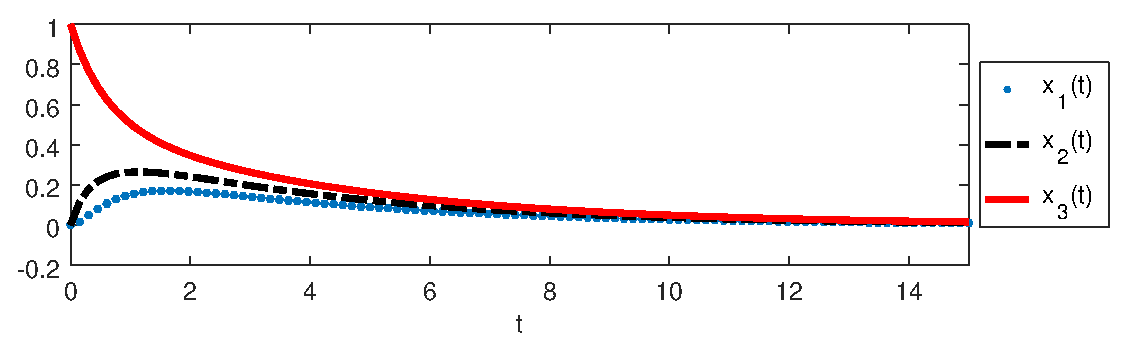
\includegraphics[width=0.99\textwidth]{chapters/differential-eq/mfiles/primeiroorder/primeirooder1.eps}
         \caption{Resposta $\VECTOR{x}(t)$ do Exemplo \ref{ex:ddxPx:0}.}
         \label{fig:ex:dxPx:0}
     \end{figure}


%%%%%%%%%%%%%%%%%%%%%%%%%%%%%%%%%%%%%%%%%%%%%%%%%%%%%%%%%%%%%%%%%%%%%%%%%%%%%%%%
\newpage
%%%%%%%%%%%%%%%%%%%%%%%%%%%%%%%%%%%%%%%%%%%%%%%%%%%%%%%%%%%%%%%%%%%%%%%%%%%%%%%%%%%%%%%
%%%%%%%%%%%%%%%%%%%%%%%%%%%%%%%%%%%%%%%%%%%%%%%%%%%%%%%%%%%%%%%%%%%%%%%%%%%%%%%%%%%%%%%
%%%%%%%%%%%%%%%%%%%%%%%%%%%%%%%%%%%%%%%%%%%%%%%%%%%%%%%%%%%%%%%%%%%%%%%%%%%%%%%%%%%%%%%
\section{ Solução da equação $\DDTVECTOR{x}(t) + \MATRIX{P} \VECTOR{x}(t)=0$ }

\begin{theorem}[Equação 
$\DDTVECTOR{x}(t) + \MATRIX{P} \VECTOR{x}(t)=0$ com matriz $\MATRIX{P}$ definida positiva:]
\label{theo:differential-eq:0}
Dados, o vetor coluna $\VECTOR{x} \in \mathbb{R}^N$, 
a \hyperref[def:positivematrix0]{\textbf{matriz definida positiva}} $\MATRIX{P} \in \mathbb{R}^{N\times N}$,
com $N$ autovalores $\lambda_n$ ``diferentes'' e seus correspondentes autovetores $\VECTOR{v}_n$,
$\forall n \in \{1, 2, ..., N\}$, 
e definida a equação diferencial matricial,
\begin{equation}\label{eq:theo:segundoorder:1}
\DDTVECTOR{x}(t) + \MATRIX{P} \VECTOR{x}(t)=0.
\end{equation}

A solução\footnote{A
demostração pode ser vista na Prova \ref{proof:theo:differential-eq:0}.} desta equação diferencial tem  a forma,
\begin{equation}\label{eq:theo:segundoorder:2}
 \VECTOR{x}(t)= \MATRIX{V}\left[\MATRIX{D}_1 cos(\VECTOR{w}t) + \MATRIX{D}_2 sin(\VECTOR{w}t) \right].
\end{equation}
\begin{itemize}
\item \textbf{Desconhecidos:} São incógnitas as matrizes diagonais $\MATRIX{D}_1 \in \mathbb{R}^{N \times N}$ e $\MATRIX{D}_2  \in \mathbb{R}^{N \times N}$, e
\item  \textbf{Conhecidos:} São definidos $\MATRIX{V}=
\begin{bmatrix}
\VECTOR{v}_1 & \VECTOR{v}_2 & \dots & \VECTOR{v}_N
\end{bmatrix}$, 
$\VECTOR{w}=
\begin{bmatrix}
\sqrt{\lambda_1} & \sqrt{\lambda_2} & \dots & \sqrt{\lambda_N}
\end{bmatrix}^{\transpose}$.
\end{itemize}
\end{theorem}

\begin{corollary}[Forma alternativa da solução do Teorema \ref{theo:differential-eq:0}:]
\label{coro:differential-eq:0}
Outra forma de escrever a Eq. (\ref{eq:theo:segundoorder:2}) é usando $\MATRIX{D}_1=\funcdiag(\VECTOR{d}_1)$ e $\MATRIX{D}_2=\funcdiag(\VECTOR{d}_2)$, de modo que
\begin{equation}\label{eq:coro:segundoorder:1}
 \VECTOR{x}(t)= \MATRIX{V}\left[ \funcdiag(cos(\VECTOR{w}t))\VECTOR{d}_1 +  \funcdiag(sin(\VECTOR{w}t)) \VECTOR{d}_2 \right],
\end{equation}
\end{corollary}

\begin{corollary}[Calculando $\MATRIX{D}_1$ e $\MATRIX{D}_2$ desde $\VECTOR{x}(t_1)$ e $\VECTOR{x}(t_2)$ na solução do Teorema \ref{theo:differential-eq:0}:]
\label{coro:differential-eq:1}
Conhecida a Eq. (\ref{eq:theo:segundoorder:2}) e o Corolário \ref{coro:differential-eq:0},
podemos calcular
$\MATRIX{D}_1=\funcdiag(\VECTOR{d}_1)$ e $\MATRIX{D}_2=\funcdiag(\VECTOR{d}_2)$ 
usando os dados $\VECTOR{x}(t_1)$ e $\VECTOR{x}(t_2)$, de modo que
\begin{equation}\label{eq:coro:differential-eq:1:a}
\begin{bmatrix}
\VECTOR{d}_1\\
\VECTOR{d}_2
\end{bmatrix}
=
\begin{bmatrix}
\MATRIX{V} \funcdiag(cos(\VECTOR{w}t_1)) &  \MATRIX{V} \funcdiag(sin(\VECTOR{w}t_1))\\
\MATRIX{V} \funcdiag(cos(\VECTOR{w}t_2)) &  \MATRIX{V} \funcdiag(sin(\VECTOR{w}t_2))
\end{bmatrix}^{-1}
\begin{bmatrix}
\VECTOR{x}(t_1)\\
\VECTOR{x}(t_2)
\end{bmatrix}
\end{equation}
\end{corollary}

\begin{corollary}[Calculando 
$\MATRIX{D}_1$ e $\MATRIX{D}_2$ desde $\VECTOR{x}(t_1)$ e $\VECTOR{\dot{x}}(t_1)$ na solução do Teorema \ref{theo:differential-eq:0}:]
\label{coro:differential-eq:2}
Conhecida a Eq. (\ref{eq:theo:segundoorder:2}) e o Corolário \ref{coro:differential-eq:0},
podemos calcular
$\MATRIX{D}_1=\funcdiag(\VECTOR{d}_1)$ e $\MATRIX{D}_2=\funcdiag(\VECTOR{d}_2)$ 
usando os dados $\VECTOR{x}(t_1)$ e $\VECTOR{\dot{x}}(t_1))$, de modo que
\begin{equation}\label{eq:coro:differential-eq:2:1}
\begin{bmatrix}
\VECTOR{d}_1\\
\VECTOR{d}_2
\end{bmatrix}
=
\begin{bmatrix}
\MATRIX{V} \funcdiag(cos(\VECTOR{w}t_1)) &  \MATRIX{V} \funcdiag(sin(\VECTOR{w}t_1))\\
-\MATRIX{V}\MATRIX{W} \funcdiag(sin(\VECTOR{w}t_1)) &  \MATRIX{V}\MATRIX{W}\funcdiag(cos(\VECTOR{w}t_1))
\end{bmatrix}^{-1}
\begin{bmatrix}
\VECTOR{x}(t_1)\\
\VECTOR{\dot{x}}(t_1)
\end{bmatrix}
\end{equation}
\end{corollary}

%%%%%%%%%%%%%%%%%%%%%%%%%%%%%%%%%%%%%%%%%%%%%%%%%%%%%%%%%%%%%%%%%%%%%%%%%%%%%%%%
\subsection{Exemplos da solução da equação $\DDTVECTOR{x}(t) + \MATRIX{P} \VECTOR{x}(t)=0$}

\begin{example}[Procurando a resposta 
$\VECTOR{x}(t)$ usando o Teorema \ref{theo:differential-eq:0}:]
\label{ex:ddxPx:0}
Calcular o vetor $\VECTOR{x}(t)$,
conhecida a equação diferencial, $\DDTVECTOR{x}(t) + \MATRIX{P} \VECTOR{x}(t)=0$, com 
um vetor $\VECTOR{x} \in \mathbb{R}^{N}$, uma matriz $\MATRIX{P}$ e as amostras $\VECTOR{x}(0)$ e $\VECTOR{\dot{x}}(0)$,
\begin{equation}
\MATRIX{P}=
\begin{bmatrix}
3 & -2 & 0\\
-2 & 3 & -1\\
0 & -1 & 1
\end{bmatrix}
\qquad \wedge \qquad
\VECTOR{x}(0)=
\begin{bmatrix}
0\\
0\\
1
\end{bmatrix}
\qquad \wedge \qquad
\VECTOR{\dot{x}}(0)=
\begin{bmatrix}
0\\
0\\
0
\end{bmatrix} 
\end{equation}
\end{example}

\newpage
\begin{SolutionT}[Relativa ao Exemplo \ref{ex:ddxPx:0}:]
\label{ex:ddxPx:0:sol1}
Sabendo que $\lambda_{\MATRIX{P}}$ e $\MATRIX{V}$ são matrizes correspondentes aos autovalores e os autovetores de $\MATRIX{P}$,
respetivamente; 
\begin{equation}
\lambda_{\MATRIX{P}}=
\begin{bmatrix}
   0.23844 &       0 &       0\\
         0 & 1.63667 &       0\\
         0 &       0 & 5.12489
\end{bmatrix}
\qquad \wedge \qquad
\MATRIX{V}=
\begin{bmatrix}
  -0.40181 & 0.61887 &-0.67495\\
  -0.55481 & 0.42186 & 0.71709\\
  -0.72852 &-0.66260 &-0.17385
\end{bmatrix},
\end{equation}
e dado que a matriz $\MATRIX{P}$ é simétrica, podemos usar o Teorema \ref{theo:positivematrix1}
para declarar que esta é definida positiva. 
onde $\MATRIX{W}=\sqrt{\lambda_{\MATRIX{P}}}$.
Assim, usando a Eq. (\ref{eq:coro:differential-eq:2:1}) do Corolário \ref{coro:differential-eq:2},
obtemos
\begin{equation}
\VECTOR{d}_1=
\begin{bmatrix}
  -0.72852\\
  -0.66260\\
  -0.17385
\end{bmatrix}
\qquad \wedge \qquad
\VECTOR{d}_2=
\begin{bmatrix}
   0\\
   0\\
   0
\end{bmatrix}
\end{equation}
de modo que 
\begin{equation}
 \VECTOR{x}(t)= 
\begin{bmatrix}
   0.292724 &-0.410061 & 0.117337\\
   0.404188 &-0.279524 &-0.124664\\
   0.530738 & 0.439039 & 0.030222
\end{bmatrix}
\begin{bmatrix}
   cos(0.48831 t)\\
   cos(1.27932 t)\\
   cos(2.26382 t)
\end{bmatrix}
\end{equation}
A Figura \ref{fig:ex:ddxPx:0} mostra um gráfico do vetor $\VECTOR{x}(t)$.
\end{SolutionT}
     \begin{figure}[!h]
         \centering
         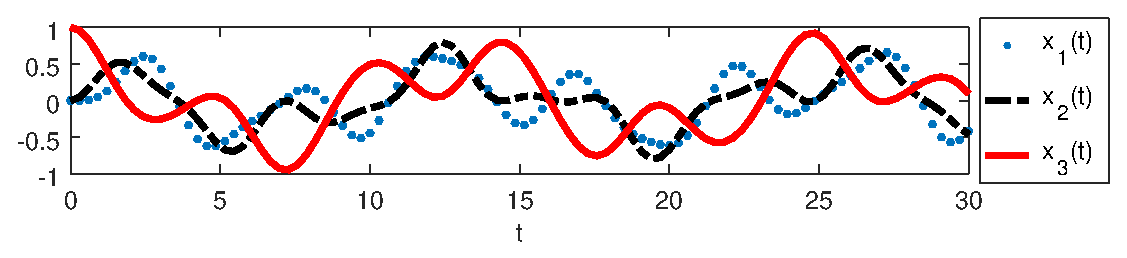
\includegraphics[width=0.99\textwidth]{chapters/differential-eq/mfiles/segundoorder/segundoroder1.eps}
         \caption{Resposta $\VECTOR{x}(t)$ do Exemplo \ref{ex:ddxPx:0}.}
         \label{fig:ex:ddxPx:0}
     \end{figure}


%%%%%%%%%%%%%%%%%%%%%%%%%%%%%%%%%%%%%%%%%%%%%%%%%%%%%%%%%%%%%%%%%%%%%%%%%%%%%%%%
\newpage
\section{Provas dos teoremas}


%%%%%%%%%%%%%%%%%%%%%%%%%%%%%%%%%%%%%%%%%%%%%%%%%%%%%%%%%%%%%%%%%%%%%%%%%%%%%%%%%%%%%%%
%%%%%%%%%%%%%%%%%%%%%%%%%%%%%%%%%%%%%%%%%%%%%%%%%%%%%%%%%%%%%%%%%%%%%%%%%%%%%%%%%%%%%%%
\begin{myproofT}[Relativa ao Teorema \ref{theo:differential-eq:order1:0}:]\label{proof:theo:differential-eq:order1:0}
Dados o vetor coluna $\VECTOR{X} \in \mathbb{R}^N$, 
a \hyperref[def:diagonalization0]{\textbf{matriz diagonalizável}} $\MATRIX{P} \in \mathbb{R}^{N\times N}$,
com $N$ autovalores $\lambda_n$ e seus correspondentes autovetores $\VECTOR{v}_n$,
$\forall n \in \{1, 2, ..., N\}$, 
e definida a equação diferencial matricial,
\begin{equation}\label{eq:firstorder1}
\DTVECTOR{X}(t) + \MATRIX{P} \VECTOR{X}(t)=0.
\end{equation}

Ela pode ser resolvida se definirmos uma resposta $\VECTOR{X}(t)$ da forma, 
\begin{equation}\label{eq:firstorder:1}
\VECTOR{X}(t)=\MATRIX{C}e^{\VECTOR{b}t},
\end{equation}
em que $\MATRIX{C} \in \mathbb{R}^{N\times N}$ é uma matriz quadrada e $\VECTOR{b} \in \mathbb{R}^{N}$ é um vetor coluna.
De modo que se introduzimos a Eq. (\ref{eq:firstorder:1}) na Eq. (\ref{eq:firstorder1}),
obtemos 
\begin{equation}\label{eq:firstorder:2}
\left(\MATRIX{C}\MATRIX{B}+\MATRIX{P}\MATRIX{C}\right)e^{\VECTOR{b}t} = 0 
\qquad \leftrightarrow \qquad
\MATRIX{B}=-\MATRIX{C}^{-1}\MATRIX{P}\MATRIX{C};
\end{equation}
em que $\MATRIX{B}=\funcdiag(\VECTOR{b})$. 
Assim, dado que $\MATRIX{B}$ é uma matriz diagonal criada pela diagonalização da  
matriz $-\MATRIX{P}$, nós sabemos que
a diagonal da matriz $\MATRIX{B}$ corresponde com os autovalores da matriz $-\MATRIX{P}$,
e seguindo o Teorema \ref{theo:diagonalization1}, a matriz $\MATRIX{C}$ é uma matriz cujas colunas estão formadas pelos 
autovetores de $\MATRIX{P}$ \cite[pp. 67]{golub2013matrix}; de modo que
\begin{equation}\label{eq:firstorder:4}
\MATRIX{B}=-
\begin{bmatrix}
\lambda_1 & 0         & ...    & 0 \\
0         & \lambda_2 & ...    & 0 \\
\vdots    & \vdots    & \ddots & \vdots \\
0         & 0         & ...    & \lambda_N
\end{bmatrix}
%\equiv -\MATRIX{C}^{-1}\MATRIX{P}\MATRIX{C}, 
\qquad \wedge \qquad 
\MATRIX{C}=\MATRIX{V}\MATRIX{D}, 
\end{equation}
em que $\MATRIX{V}=\left[ \VECTOR{v}_1~  \VECTOR{v}_2~  \dots~ \VECTOR{v}_N\right]$ 
é uma matriz formada pela agrupação dos autovetores $\VECTOR{v}_n$ da matriz $\MATRIX{P}$,
e $\MATRIX{D}=\funcdiag\left(\left[ d_1~  d_2~  \dots~ d_N\right]\right)$ 
é uma matriz diagonal, de modo que podemos formar outra matriz  
$\MATRIX{V}\MATRIX{D}=\left[ d_1\VECTOR{v}_1~  d_2\VECTOR{v}_2~  \dots~ d_N\VECTOR{v}_N\right]$
com autovetores nas colunas.
Assim, a Eq. (\ref{eq:firstorder:4}) gera uma solução para a Eq. (\ref{eq:firstorder1}),
em que é possível afirmar que
\begin{equation}\label{eq:firstorder:5}
\VECTOR{X}(t)=\MATRIX{V}\MATRIX{D} e^{-\VECTOR{a} t},
\end{equation}
sendo $\VECTOR{a}=\left[ \lambda_1~ \lambda_2~ \dots~ \lambda_M\right]^{T}$.
\end{myproofT}

%%%%%%%%%%%%%%%%%%%%%%%%%%%%%%%%%%%%%%%%%%%%%%%%%%%%%%%%%%%%%%%%%%%%%%%%%%%%%%%%%%%%%%%
%%%%%%%%%%%%%%%%%%%%%%%%%%%%%%%%%%%%%%%%%%%%%%%%%%%%%%%%%%%%%%%%%%%%%%%%%%%%%%%%%%%%%%%
\begin{myproofT}[Relativa ao Teorema \ref{theo:differential-eq:0}:]\label{proof:theo:differential-eq:0}
Dados o vetor coluna $\VECTOR{X} \in \mathbb{R}^N$, 
a \hyperref[def:positivematrix0]{\textbf{matriz definida positiva}} $\MATRIX{P} \in \mathbb{R}^{N\times N}$,
com $N$ autovalores $\lambda_n$ ``diferentes'' e seus correspondentes autovetores $\VECTOR{v}_n$,
$\forall n \in \{1, 2, ..., N\}$, 
e definida a equação diferencial matricial,
\begin{equation}\label{eq:segundoorder1}
\DDTVECTOR{X}(t) + \MATRIX{P} \VECTOR{X}(t)=0.
\end{equation}

Ela pode ser resolvida se definirmos uma resposta $\VECTOR{X}(t)$ da forma, 
\begin{equation}\label{eq:segundoorder:1}
\VECTOR{X}(t)=\MATRIX{C}e^{\VECTOR{b}t},
\end{equation}
em que $\MATRIX{C} \in \mathbb{C}^{N\times N}$ é uma matriz quadrada e $\VECTOR{b} \in \mathbb{C}^{N}$ é um vetor coluna.
De modo que se introduzimos a Eq. (\ref{eq:segundoorder:1}) na Eq. (\ref{eq:segundoorder1}),
obtemos 
\begin{equation}\label{eq:segundoorder:2}
\left(\MATRIX{C}\MATRIX{B}^2+\MATRIX{P}\MATRIX{C}\right)e^{\VECTOR{b}t} = 0 
\qquad \leftrightarrow \qquad
\MATRIX{B}^2=-\MATRIX{C}^{-1}\MATRIX{P}\MATRIX{C};
\end{equation}

em que $\MATRIX{B}=\funcdiag(\VECTOR{b})$. 
Assim, dado que $\MATRIX{B}^2$ é uma matriz diagonal criada pela diagonalização da  
matriz $-\MATRIX{P}$, nós sabemos que
a diagonal da matriz $\MATRIX{B}^2$ corresponde com os autovalores da matriz $-\MATRIX{P}$,
e seguindo o Teorema \ref{theo:diagonalization1}, a matriz $\MATRIX{C}$ é uma matriz cujas colunas estão formadas pelos 
autovetores de $\MATRIX{P}$ \cite[pp. 67]{golub2013matrix}; de modo que
\begin{equation}\label{eq:segundoorder:4}
\MATRIX{B}^2=-
\begin{bmatrix}
\lambda_1 & 0         & ...    & 0 \\
0         & \lambda_2 & ...    & 0 \\
\vdots    & \vdots    & \ddots & \vdots \\
0         & 0         & ...    & \lambda_N
\end{bmatrix}
%\equiv -\MATRIX{C}^{-1}\MATRIX{P}\MATRIX{C}, 
\qquad \wedge \qquad \MATRIX{C}=\MATRIX{V}\MATRIX{A}, 
\end{equation}
onde $\MATRIX{V}=\left[ \VECTOR{v}_1~  \VECTOR{v}_2~  \dots~ \VECTOR{v}_N\right]$ 
é uma matriz formada pela agrupação dos autovetores $\VECTOR{v}_n$ da matriz $\MATRIX{P}$,
e $\MATRIX{A}=\funcdiag\left(\left[ a_1~  a_2~  \dots~ a_N\right]\right)$ 
é uma matriz diagonal para formar outra matriz  
$\MATRIX{V}\MATRIX{A}=\left[ a_1\VECTOR{v}_1~  a_2\VECTOR{v}_2~  \dots~ a_N\VECTOR{v}_N\right]$
com autovetores nas colunas.
Assim, a Eq. (\ref{eq:segundoorder:4}) gera um par de soluções para a Eq. (\ref{eq:segundoorder1}),
onde é possível afirmar que
\begin{equation}\label{eq:segundoorder:5}
\VECTOR{X}(t)=\MATRIX{V}\MATRIX{A}_1 e^{\VECTOR{w} \mathbf{i} t}+ \MATRIX{V}\MATRIX{A}_2 e^{-\VECTOR{w} \mathbf{i} t},
\end{equation}
onde $\VECTOR{w}=\left[ \sqrt{\lambda_1}~ \sqrt{\lambda_2}~ \dots~ \sqrt{\lambda_M}\right]^{T}$, 
e $\MATRIX{A}_1$ e $\MATRIX{A}_2$ são duas matrizes diagonais qualquer.
Se reordenamo a Eq. (\ref{eq:segundoorder:5}) obtemos
\begin{equation}\label{eq:segundoorder:6}
\VECTOR{X}(t)=
\MATRIX{V}\left(\MATRIX{A}_1+\MATRIX{A}_2\right) cos\left(\VECTOR{w}  t\right)+ 
\MATRIX{V}\left(\MATRIX{A}_1-\MATRIX{A}_2\right) \mathbf{i} sin\left(\VECTOR{w}  t\right);
\end{equation}
dado que soubemos que a resposta $\VECTOR{X}(t)$ é real, 
podemos afirmar que $\MATRIX{A}_1$ é uma matriz complexa conjugada da matriz $\MATRIX{A}_2$,
de modo que podemos rescrever a Eq. (\ref{eq:segundoorder:6}) como
\begin{equation}\label{eq:segundoorder:7}
 \VECTOR{X}(t)= \MATRIX{V}\left[\MATRIX{D}_1 cos(\VECTOR{w}t) + \MATRIX{D}_2 sin(\VECTOR{w}t) \right],
\end{equation}
onde $\MATRIX{D}_1 \in \mathbb{R}^{N\times N}$ e $\MATRIX{D}_2 \in \mathbb{R}^{N\times N}$ 
são matrizes diagonais reais. 
\end{myproofT}



\chapterimage{chapter_derivada.pdf} % Chapter heading image

\chapter{Solução iterativa de equações diferenciais matriciais}% de funções $\VECTOR{x}[n]$: $\mathbb{R}^{N}$}


%%%%%%%%%%%%%%%%%%%%%%%%%%%%%%%%%%%%%%%%%%%%%%%%%%%%%%%%%%%%%%%%%%%%%%%%%%%%%%%%
%%%%%%%%%%%%%%%%%%%%%%%%%%%%%%%%%%%%%%%%%%%%%%%%%%%%%%%%%%%%%%%%%%%%%%%%%%%%%%%%%%%%%%%
%%%%%%%%%%%%%%%%%%%%%%%%%%%%%%%%%%%%%%%%%%%%%%%%%%%%%%%%%%%%%%%%%%%%%%%%%%%%%%%%%%%%%%%
%%%%%%%%%%%%%%%%%%%%%%%%%%%%%%%%%%%%%%%%%%%%%%%%%%%%%%%%%%%%%%%%%%%%%%%%%%%%%%%%%%%%%%%
\section{Diferenças finitas}

O método das diferenças finitas nos brinda com uma ferramenta para a resolução de 
equações diferenciais; com esse fim são utilizadas aproximações das derivadas\footnote{As 
derivadas são diferencias infinitesimais.} 
mediante diferenças finitas.

\begin{definition}[Amostragem de uma função:]
\label{def:diferenças-finitas:0}
Dado um conjunto de amostras de um sinal representado pela função $\VECTOR{f}: \mathbb{R} \rightarrow \mathbb{R}^N$, 
adquiridas nos  tempos $t_n$, $\forall n \in \mathbb{Z}$; 
se essas amostras foram adquiridas de forma regular a cada $\ToS$ segundos,
então podemos definir que
\begin{equation}
\VECTOR{f}(t_n)\equiv \VECTOR{f}(n\tau) \equiv \VECTOR{f}[n].
\end{equation}
\end{definition}

\begin{theorem}[Diferença finita para derivada segunda:]
\label{teo:diferenças-finitas:2}
Usando a \hyperref[def:taylor]{\textbf{série de Taylor}}, podemos aproximar 
a segunda derivada de uma função $\VECTOR{f}(t)$, em que\footnote{A
demonstração da aproximação e o erro do cálculo podem ser visto na Prova \ref{proof:teo:diferenças-finitas:2}.}
\begin{equation}
\left.\frac{d^2\VECTOR{f}(t)}{dt^2}\right|_{t=t_n}\equiv \DDTVECTOR{f}(t_n)
\quad \approx \quad
%\frac{\VECTOR{f}(t_n+\ToS)-2\VECTOR{f}(t_n)+\VECTOR{f}(t_n-\ToS)}{\ToS^2} \equiv 
\frac{\VECTOR{f}[n+1]-2\VECTOR{f}[n]+\VECTOR{f}[n-1]}{\ToS^2}.
\end{equation}
\end{theorem}

\begin{tcbattention}
\begin{itemize}
\item Para um valor $\ToS$, tal que $0<|\ToS|<1$, a aproximação da primeira derivada por diferença finita, 
que produz o menor erro, é a que usa ``diferença central'', pois o erro é proporcional a ${\ToS}^2$ 
(Ver Teorema \ref{teo:diferenças-finitas:1}
e a Prova \ref{proof:teo:diferenças-finitas:1}); porém, 
essa aproximação tem o problema de necessitar de amostras futuras para dar um parecer da amostra atual.
\item As aproximações por diferenças progressivas e regressivas têm erros comparáveis
 (Ver Prova \ref{proof:teo:diferenças-finitas:1});
porém as diferenças regressivas têm como vantagem que, para dar um parecer da amostra atual,
você só precisa de amostras anteriores.
\end{itemize}
\end{tcbattention}


\begin{theorem}[Diferença finita para a primeira derivada:]
\label{teo:diferenças-finitas:1}
Usando a \hyperref[def:taylor]{\textbf{série de Taylor}}, podemos aproximar\footnote{As
demonstrações das aproximações e o erro do cálculo podem ser visto na Prova \ref{proof:teo:diferenças-finitas:1}.} 
a primeira derivada de uma função $\VECTOR{f}(t)$.
\begin{itemize}
\item \textbf{Diferença regressiva ou atrasada:}
\begin{equation}
\left.\frac{d\VECTOR{f}(t)}{dt}\right|_{t=t_n}\equiv \DTVECTOR{f}(t_n)
\quad \approx \quad
%\frac{\VECTOR{f}(t_n)-\VECTOR{f}(t_n-\ToS)}{\ToS} \equiv 
\frac{\VECTOR{f}[n]-\VECTOR{f}[n-1]}{\ToS}
\end{equation}
\item \textbf{Diferença progressiva:}
\begin{equation}
\left.\frac{d\VECTOR{f}(t)}{dt}\right|_{t=t_n}\equiv \DTVECTOR{f}(t_n)
\quad \approx \quad
%\frac{\VECTOR{f}(t_n)-\VECTOR{f}(t_n-\ToS)}{\ToS} \equiv 
\frac{\VECTOR{f}[n+1]-\VECTOR{f}[n]}{\ToS}
\end{equation}
\item \textbf{Diferença central:}
\begin{equation}
\left.\frac{d\VECTOR{f}(t)}{dt}\right|_{t=t_n}\equiv \DTVECTOR{f}(t_n)
\quad \approx \quad
%\frac{\VECTOR{f}(t_n)-\VECTOR{f}(t_n-\ToS)}{\ToS} \equiv 
\frac{\VECTOR{f}[n+1]-\VECTOR{f}[n-1]}{2\ToS}
\end{equation}
\end{itemize}
\end{theorem}



%% polinomios interpoladores
%https://www.ufrgs.br/reamat/CalculoNumerico/livro-sci/dn-obtencao_de_formulas_por_polinomios_interpoladores.html


%%%%%%%%%%%%%%%%%%%%%%%%%%%%%%%%%%%%%%%%%%%%%%%%%%%%%%%%%%%%%%%%%%%%%%%%%%%%%%%%
\newpage
%%%%%%%%%%%%%%%%%%%%%%%%%%%%%%%%%%%%%%%%%%%%%%%%%%%%%%%%%%%%%%%%%%%%%%%%%%%%%%%%%%%%%%%
%%%%%%%%%%%%%%%%%%%%%%%%%%%%%%%%%%%%%%%%%%%%%%%%%%%%%%%%%%%%%%%%%%%%%%%%%%%%%%%%%%%%%%%
%%%%%%%%%%%%%%%%%%%%%%%%%%%%%%%%%%%%%%%%%%%%%%%%%%%%%%%%%%%%%%%%%%%%%%%%%%%%%%%%%%%%%%%
\section{ Solução iterativa da equação $\DTVECTOR{x}(t) + \MATRIX{P} \VECTOR{x}(t)=0$ }

\begin{theorem}[Equação 
$\DTVECTOR{x}(t) + \MATRIX{P} \VECTOR{x}(t)=0$ com diferenças regressivas:]
\label{theo:differential-eq-discreto:order1:0}
Dados, o vetor coluna $\VECTOR{x} \in \mathbb{R}^N$, matriz $\MATRIX{P} \in \mathbb{R}^{N\times N}$, 
e definida a equação diferencial matricial,
\begin{equation}
\DTVECTOR{x}(t) + \MATRIX{P} \VECTOR{x}(t)=0.
\end{equation}
A solução\footnote{A
demostração pode ser vista na Prova \ref{proof:theo:differential-eq-discreto:order1:0}.} desta equação diferencial tem  a forma,
\begin{equation}
  \VECTOR{x}[n]=\left\{\MATRIX{I} + \ToS \MATRIX{P}\right\}^{-1}\VECTOR{x}[n-1],
\end{equation}
onde $\MATRIX{I}$ é uma matriz identidade.
\begin{itemize}
\item \textbf{Desconhecidos:} Um valor inicial, por exemplo $\VECTOR{x}[0] \in \mathbb{R}^{N}$.
\item  \textbf{Conhecidos:} É escolhido por nós um valor $\ToS$, 
que é a frequencia de amostragem da sinal discreta $\VECTOR{x}[n]$.
\end{itemize}
\end{theorem}

\begin{tcbattention}
\begin{itemize}
\item O valor de $\ToS$ deve ser escolhido tomando em conta o teorema de Nyquist (teorema da amostragem) 
\cite[pp. 67]{rochol2009comunicacao} \cite[pp. 122]{forouzan2009comunicacao}.
\end{itemize}
\end{tcbattention}

%%%%%%%%%%%%%%%%%%%%%%%%%%%%%%%%%%%%%%%%%%%%%%%%%%%%%%%%%%%%%%%%%%%%%%%%%%%%%%%%
\subsection{Exemplos da solução iterativa da equação $\DTVECTOR{x}(t) + \MATRIX{P} \VECTOR{x}(t)=0$}

\begin{example}[Procurando uma resposta iterativa usando o Teorema \ref{theo:differential-eq-discreto:order1:0}:]
\label{ex:iterativo:dxPx:0}
Calcular o vetor $\VECTOR{x}[n] \in \mathbb{R}^{N}$,
conhecida a equação diferencial, $\DTVECTOR{x}(t) + \MATRIX{P} \VECTOR{x}(t)=0$, e
\begin{equation}
\MATRIX{P}=
\begin{bmatrix}
3 & -2 & 0\\
-2 & 3 & -1\\
0 & -1 & 1
\end{bmatrix}
\qquad \wedge \qquad
\VECTOR{x}[0]=
\begin{bmatrix}
0\\
0\\
1
\end{bmatrix}.
\end{equation}
\end{example}


\begin{SolutionT}[Relativa ao Exemplo \ref{ex:iterativo:dxPx:0}:]
\label{ex:iterativo:dxPx:0:sol1}
Escolhemos uma frequencia de amostragem $\ToS=0.1$, e
tomamos amostras $\VECTOR{x}(t_n)$, para $n \in \{0,~ 1,~ 2,~ ...,~ 150\}$, 
de modo que usando o Teorema \ref{theo:differential-eq-discreto:order1:0} obtemos a Eq. (\ref{eq:iterativo:dxPx:0:sol1}),
e podemos calcular a função $\VECTOR{x}(t_n)$ mostrada na Figura \ref{fig:ex:iterativo:dxPx:0}.
\begin{equation}\label{eq:iterativo:dxPx:0:sol1}
\MATRIX{A}=
\left\{\MATRIX{I} + \ToS \MATRIX{P}\right\}^{-1}=
\begin{bmatrix}
   0.788013 & 0.122087 & 0.011099 \\
   0.122087 & 0.793563 & 0.072142 \\
   0.011099 & 0.072142 & 0.915649 
\end{bmatrix}
\qquad \rightarrow \qquad
\VECTOR{x}[n]=\MATRIX{A} \VECTOR{x}[n-1].
\end{equation}

\end{SolutionT}
     \begin{figure}[!h]
         \centering
         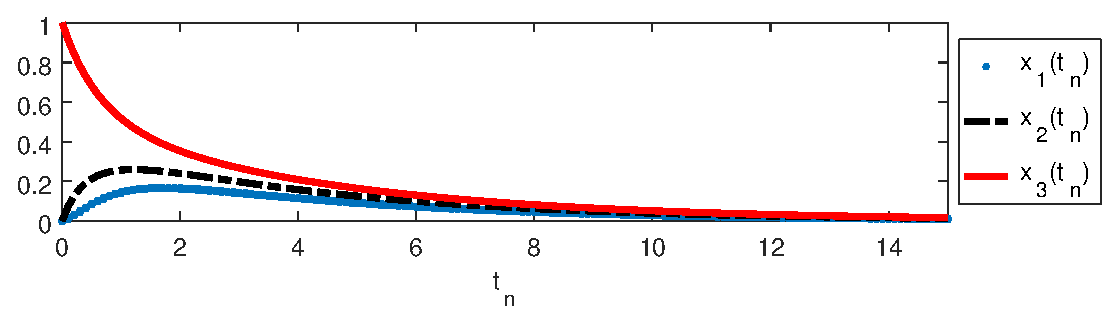
\includegraphics[width=0.89\textwidth]{chapters/differential-eq-discreto/mfiles/primeiroorder/primeirooder1.eps}
         \caption{Resposta $\VECTOR{x}(t)$ do Exemplo \ref{ex:ddxPx:0}.}
         \label{fig:ex:iterativo:dxPx:0}
     \end{figure}


%%%%%%%%%%%%%%%%%%%%%%%%%%%%%%%%%%%%%%%%%%%%%%%%%%%%%%%%%%%%%%%%%%%%%%%%%%%%%%%%
\newpage
%%%%%%%%%%%%%%%%%%%%%%%%%%%%%%%%%%%%%%%%%%%%%%%%%%%%%%%%%%%%%%%%%%%%%%%%%%%%%%%%%%%%%%%
%%%%%%%%%%%%%%%%%%%%%%%%%%%%%%%%%%%%%%%%%%%%%%%%%%%%%%%%%%%%%%%%%%%%%%%%%%%%%%%%%%%%%%%
%%%%%%%%%%%%%%%%%%%%%%%%%%%%%%%%%%%%%%%%%%%%%%%%%%%%%%%%%%%%%%%%%%%%%%%%%%%%%%%%%%%%%%%
\section{ Solução iterativa da equação $\DDTVECTOR{x}(t) + \MATRIX{P} \VECTOR{x}(t)=0$ }

\begin{theorem}[Equação 
$\DDTVECTOR{x}(t) + \MATRIX{P} \VECTOR{x}(t)=0$ com diferenças finitas:]
\label{theo:differential-eq-discreto:order2:0}
Dados o vetor coluna $\VECTOR{x} \in \mathbb{R}^N$, a matriz $\MATRIX{P} \in \mathbb{R}^{N\times N}$, 
e definida a equação diferencial matricial,
\begin{equation}\label{eq:theo:secondorder:1}
\DDTVECTOR{x}(t) + \MATRIX{P} \VECTOR{x}(t)=0.
\end{equation}
A solução\footnote{A
demonstração pode ser vista na Prova \ref{proof:theo:differential-eq-discreto:order2:0}.} dessa 
equação diferencial tem  a forma,
\begin{equation}\label{eq:theo:secondorder:2}
  \VECTOR{x}[n]=\left\{2\MATRIX{I} - \ToS^2 \MATRIX{P}\right\}\VECTOR{x}[n-1]-\VECTOR{x}[n-2],
\end{equation}
em que $\MATRIX{I}$ é uma matriz identidade.
\begin{itemize}
\item \textbf{Desconhecidos:} Dois valores iniciais consecutivos, 
por exemplo $\VECTOR{x}[0],\VECTOR{x}[1] \in \mathbb{R}^{N}$, e
\item  \textbf{Conhecidos:} É escolhido por nós um valor $\ToS$, 
que é a frequência de amostragem do sinal discreta $\VECTOR{x}[n]$.
\end{itemize}
\end{theorem}

\begin{tcbattention}
\begin{itemize}
\item O valor de $\ToS$ deve ser escolhido tomando em conta o teorema de Nyquist (teorema da amostragem) 
\cite[pp. 67]{rochol2009comunicacao} \cite[pp. 122]{forouzan2009comunicacao}.
\end{itemize}
\end{tcbattention}

%%%%%%%%%%%%%%%%%%%%%%%%%%%%%%%%%%%%%%%%%%%%%%%%%%%%%%%%%%%%%%%%%%%%%%%%%%%%%%%%
\subsection{Exemplos da solução iterativa da equação $\DDTVECTOR{x}(t) + \MATRIX{P} \VECTOR{x}(t)=0$}

\begin{example}[Procurando uma resposta iterativa usando o Teorema \ref{theo:differential-eq-discreto:order2:0}:]
\label{ex:iterativo:ddxPx:0}
Calcular o vetor $\VECTOR{x}[n] \in \mathbb{R}^{N}$,
conhecida a equação diferencial, $\DDTVECTOR{x}(t) + \MATRIX{P} \VECTOR{x}(t)=0$, e
\begin{equation}
\MATRIX{P}=
\begin{bmatrix}
3 & -2 & 0\\
-2 & 3 & -1\\
0 & -1 & 1
\end{bmatrix}
\qquad \wedge \qquad
\VECTOR{x}[0]=
\begin{bmatrix}
0\\
0\\
1
\end{bmatrix}
\qquad \wedge \qquad
\VECTOR{x}[-1]=
\begin{bmatrix}
0\\
0\\
1
\end{bmatrix}.
\end{equation}
\end{example}


\begin{SolutionT}[Relativa ao Exemplo \ref{ex:iterativo:ddxPx:0}:]
\label{ex:iterativo:ddxPx:0:sol1}
Escolhemos uma frequência de amostragem $\ToS=0.1$, e
tomamos amostras $\VECTOR{x}(t_n)$, para $n \in \{0,~ 1,~ 2,~ ...,~ 150\}$, 
de modo que usando o Teorema \ref{theo:differential-eq-discreto:order2:0}, 
obtemos a Eq. (\ref{eq:iterativo:ddxPx:0:sol1})
e podemos calcular a função $\VECTOR{x}(t_n)$ mostrada na Figura \ref{fig:ex:iterativo:ddxPx:0}.
\begin{equation}\label{eq:iterativo:ddxPx:0:sol1}
\MATRIX{A}=
2\MATRIX{I} -\ToS^2 \MATRIX{P}=
\begin{bmatrix}
   1.97000 & 0.02000 &-0.00000\\
   0.02000 & 1.97000 & 0.01000\\
  -0.00000 & 0.01000 & 1.99000
\end{bmatrix}
\qquad \rightarrow \qquad
\VECTOR{x}[n]=\MATRIX{A} \VECTOR{x}[n-1]-\VECTOR{x}[n-2].
\end{equation}
\end{SolutionT}

     \begin{figure}[!h]
         \centering
         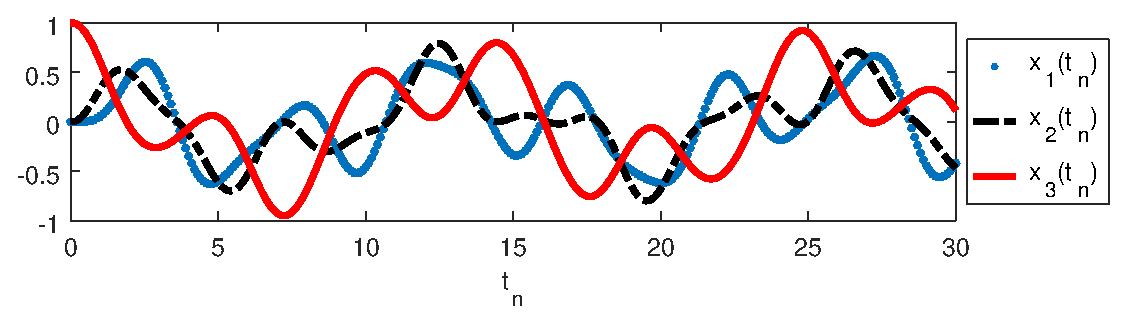
\includegraphics[width=0.89\textwidth]{chapters/differential-eq-discreto/mfiles/segundoorder/segundooder1.eps}
         \caption{Resposta $\VECTOR{x}(t)$ do Exemplo \ref{ex:ddxPx:0}.}
         \label{fig:ex:iterativo:ddxPx:0}
     \end{figure}


%%%%%%%%%%%%%%%%%%%%%%%%%%%%%%%%%%%%%%%%%%%%%%%%%%%%%%%%%%%%%%%%%%%%%%%%%%%%%%%%
\newpage
\section{Provas dos teoremas}


%%%%%%%%%%%%%%%%%%%%%%%%%%%%%%%%%%%%%%%%%%%%%%%%%%%%%%%%%%%%%%%%%%%%%%%%%%%%%%%%%%%%%%%
%%%%%%%%%%%%%%%%%%%%%%%%%%%%%%%%%%%%%%%%%%%%%%%%%%%%%%%%%%%%%%%%%%%%%%%%%%%%%%%%%%%%%%%
\begin{myproofT}[Prova do Teorema \ref{teo:diferenças-finitas:1}:]\label{proof:teo:diferenças-finitas:1}
Usando a \hyperref[def:taylor]{\textbf{serie de Taylor}} podemos aproximar 
a primeira derivada de uma função $\VECTOR{f}(t)$, onde
\begin{itemize}
\item \textbf{Diferença regressiva ou atrasada:}
\begin{equation}
\VECTOR{f}(t_n-\ToS) = \VECTOR{f}(t_n)-\DTVECTOR{f}(t_n)\ToS +\frac{\ToS^2}{2}\DDTVECTOR{f}(z_{1}^{-}),
\end{equation}
\begin{equation}
\DTVECTOR{f}(t_n)=\underbrace{\frac{\VECTOR{f}(t_n)-\VECTOR{f}(t_n-\ToS)}{\ToS}}_{\DTVECTOR{f}_{1^{-}}(t_n)}+
\underbrace{\frac{\ToS}{2}\DDTVECTOR{f}(z_{1}^{-})}_{\VECTOR{R}_{1^{-}}(z_{1}^{-},\ToS)},
\end{equation}
onde podemos afirmar que $\DTVECTOR{f}(t_n)\approx \DTVECTOR{f}_{1^{-}}(t_n)$ com um erro $\VECTOR{R}_{1^{-}}(z_{1}^{-},\ToS)$,
$z_{1}^{-} \in ]t_n-\ToS,t_n[$ quando $\ToS>0$, e $z_{1}^{+} \in ]t_n,t_n-\ToS[$ quando $\ToS<0$.

\item \textbf{Diferença progressiva:}
\begin{equation}
\VECTOR{f}(t_n+\ToS) = \VECTOR{f}(t_n)+\DTVECTOR{f}(t_n)\ToS +\frac{\ToS^2}{2}\DDTVECTOR{f}(z_{1}^{+}),
\end{equation}
\begin{equation}
\DTVECTOR{f}(t_n)=\underbrace{\frac{\VECTOR{f}(t_n+\ToS) - \VECTOR{f}(t_n)}{\ToS}}_{\DTVECTOR{f}_{1^{+}}(t_n)}-
\underbrace{\frac{\ToS}{2}\DDTVECTOR{f}(z_{1}^{+})}_{\VECTOR{R}_{1^{+}}(z_{1}^{+},\ToS)},
\end{equation}
onde podemos afirmar que $\DTVECTOR{f}(t_n)\approx \DTVECTOR{f}_{1^{+}}(t_n)$ com um erro $\VECTOR{R}_{1^{+}}(z_{1}^{+},\ToS)$,
$z_{1}^{+} \in ]t_n,t_n+\ToS[$ quando $\ToS>0$, e $z_{1}^{+} \in ]t_n+\ToS,t_n[$ quando $\ToS<0$.

\item \textbf{Diferença central:} 
\begin{equation}\label{eq:proof:teo:diferenças-finitas:1:a}
\VECTOR{f}(t_n-\ToS) = \VECTOR{f}(t_n)-\DTVECTOR{f}(t_n)\ToS +\DDTVECTOR{f}(t_n) \frac{\ToS^2}{2}-\frac{\ToS^3}{3!}\DDDTVECTOR{f}(z_{2}^{-}),
\end{equation}
\begin{equation}\label{eq:proof:teo:diferenças-finitas:1:b}
\VECTOR{f}(t_n+\ToS) = \VECTOR{f}(t_n)+\DTVECTOR{f}(t_n)\ToS +\DDTVECTOR{f}(t_n) \frac{\ToS^2}{2}+\frac{\ToS^3}{3!}\DDDTVECTOR{f}(z_{2}^{+}),
\end{equation}
restando as Eqs. (\ref{eq:proof:teo:diferenças-finitas:1:a}) e (\ref{eq:proof:teo:diferenças-finitas:1:b}) obtemos,
\begin{equation}
\VECTOR{f}(t_n+\ToS) - \VECTOR{f}(t_n-\ToS) = 2\DTVECTOR{f}(t_n)\ToS +\frac{\ToS^3}{3!}\DDDTVECTOR{f}(z_{2}^{+}) + \frac{\ToS^3}{3!}\DDTVECTOR{f}(z_{2}^{-}),
\end{equation}
\begin{equation}
\DTVECTOR{f}(t_n) = \underbrace{\frac{\VECTOR{f}(t_n+\ToS) - \VECTOR{f}(t_n-\ToS)}{2\ToS}}_{\DTVECTOR{f}_{1^{0}}(t_n)} - 
\underbrace{\frac{\ToS^2}{12} \left[\DDDTVECTOR{f}(z_{2}^{+}) + \DDDTVECTOR{f}(z_{2}^{-})\right]}_{\VECTOR{R}_{1^{0}}(z_{2}^{-},z_{2}^{+},\ToS)},
\end{equation}
onde podemos afirmar que $\DTVECTOR{f}(t_n)\approx \DTVECTOR{f}_{1^{0}}(t_n)$ 
com um erro $\VECTOR{R}_{1^{0}}(z_{2}^{-},z_{2}^{+},\ToS)$.
\end{itemize}
\end{myproofT}
%%%%%%%%%%%%%%%%%%%%%%%%%%%%%%%%%%%%%%%%%%%%%%%%%%%%%%%%%%%%%%%%%%%%%%%%%%%%%%%%%%%%%%%
%%%%%%%%%%%%%%%%%%%%%%%%%%%%%%%%%%%%%%%%%%%%%%%%%%%%%%%%%%%%%%%%%%%%%%%%%%%%%%%%%%%%%%%
\begin{myproofT}[Prova do Teorema \ref{teo:diferenças-finitas:2}:]\label{proof:teo:diferenças-finitas:2}
Usando a \hyperref[def:taylor]{\textbf{serie de Taylor}} podemos aproximar 
a segunda derivada de uma função $\VECTOR{f}(t)$.
\begin{equation}\label{eq:proof:teo:diferenças-finitas:1:a}
\VECTOR{f}(t_n-\ToS) = 
\VECTOR{f}(t_n)-\DTVECTOR{f}(t_n)\ToS +\DDTVECTOR{f}(t_n) \frac{\ToS^2}{2}-\DDDTVECTOR{f}(t_n) \frac{\ToS^3}{3!} +\frac{\ToS^4}{4!}\DDDDTVECTOR{f}(z_{3}^{-}),
\end{equation}
\begin{equation}\label{eq:proof:teo:diferenças-finitas:1:b}
\VECTOR{f}(t_n+\ToS) = 
\VECTOR{f}(t_n)+\DTVECTOR{f}(t_n)\ToS +\DDTVECTOR{f}(t_n) \frac{\ToS^2}{2}+\DDDTVECTOR{f}(t_n) \frac{\ToS^3}{3!} +\frac{\ToS^4}{4!}\DDDDTVECTOR{f}(z_{3}^{+}),
\end{equation}
somando as Eqs. (\ref{eq:proof:teo:diferenças-finitas:1:a}) e (\ref{eq:proof:teo:diferenças-finitas:1:b}) obtemos,
\begin{equation}
\VECTOR{f}(t_n-\ToS) + \VECTOR{f}(t_n+\ToS) = 2 \VECTOR{f}(t_n)+2\DDTVECTOR{f}(t_n) \frac{\ToS^2}{2}+\frac{\ToS^4}{4!}\DDDDTVECTOR{f}(z_{3}^{-}) +\frac{\ToS^4}{4!}\DDDDTVECTOR{f}(z_{3}^{+}),
\end{equation}
\begin{equation}
 \DDTVECTOR{f}(t_n) =
\underbrace{\frac{\VECTOR{f}(t_n-\ToS) -2 \VECTOR{f}(t_n) + \VECTOR{f}(t_n+\ToS)}{\ToS^2}}_{\DTVECTOR{f}_{2^{0}}(t_n)}
-\underbrace{\frac{\ToS^2}{4!}\left[\DDDDTVECTOR{f}(z_{3}^{-}) +\DDDDTVECTOR{f}(z_{3}^{+})\right]}_{\VECTOR{R}_{2^{0}}(z_{3}^{-},z_{3}^{+},\ToS)} ,
\end{equation}
\end{myproofT}



%%%%%%%%%%%%%%%%%%%%%%%%%%%%%%%%%%%%%%%%%%%%%%%%%%%%%%%%%%%%%%%%%%%%%%%%%%%%%%%%%%%%%%%
%%%%%%%%%%%%%%%%%%%%%%%%%%%%%%%%%%%%%%%%%%%%%%%%%%%%%%%%%%%%%%%%%%%%%%%%%%%%%%%%%%%%%%%
\begin{myproofT}[Prova do Teorema \ref{theo:differential-eq-discreto:order1:0}:]\label{proof:theo:differential-eq-discreto:order1:0}
Dados, o vetor coluna $\VECTOR{x} \in \mathbb{R}^N$, matriz $\MATRIX{P} \in \mathbb{R}^{N\times N}$, 
e definida a equação diferencial matricial,
\begin{equation}\label{eq:theo:firstorder:1}
\DTVECTOR{x}(t) + \MATRIX{P} \VECTOR{x}(t)=0.
\end{equation}
podemos usar as diferenças regressivas
\begin{equation}
\frac{\VECTOR{x}[n]-\VECTOR{x}[n-1]}{\ToS} + \MATRIX{P} \VECTOR{x}[n]=0.
\end{equation}
\begin{equation}
\left\{\MATRIX{I}  + \ToS \MATRIX{P}\right\} \VECTOR{x}[n]=\VECTOR{x}[n-1].
\end{equation}
\begin{equation}
\VECTOR{x}[n]=\left\{\MATRIX{I}  + \ToS \MATRIX{P}\right\}^{-1}\VECTOR{x}[n-1].
\end{equation}
\end{myproofT}

%%%%%%%%%%%%%%%%%%%%%%%%%%%%%%%%%%%%%%%%%%%%%%%%%%%%%%%%%%%%%%%%%%%%%%%%%%%%%%%%%%%%%%%
%%%%%%%%%%%%%%%%%%%%%%%%%%%%%%%%%%%%%%%%%%%%%%%%%%%%%%%%%%%%%%%%%%%%%%%%%%%%%%%%%%%%%%%
\begin{myproofT}[Prova do Teorema \ref{theo:differential-eq-discreto:order2:0}:]\label{proof:theo:differential-eq-discreto:order2:0}
Dados, o vetor coluna $\VECTOR{x} \in \mathbb{R}^N$, matriz $\MATRIX{P} \in \mathbb{R}^{N\times N}$, 
e definida a equação diferencial matricial,
\begin{equation}\label{eq:theo:firstorder:1}
\DDTVECTOR{x}(t) + \MATRIX{P} \VECTOR{x}(t)=0.
\end{equation}
podemos usar as diferenças finitas
\begin{equation}
\frac{\VECTOR{x}[n+1]-2\VECTOR{x}[n]+ \VECTOR{x}[n-1]}{\ToS^2} + \MATRIX{P} \VECTOR{x}[n]=0.
\end{equation}
\begin{equation}
\VECTOR{x}[n+1]-2\VECTOR{x}[n]+ \VECTOR{x}[n-1]  + \ToS^2 \MATRIX{P} \VECTOR{x}[n]=0.
\end{equation}
\begin{equation}
\VECTOR{x}[n+1]  =\left\{2\MATRIX{I}- \ToS^2 \MATRIX{P} \right\}\VECTOR{x}[n] - \VECTOR{x}[n-1].
\end{equation}
\end{myproofT}




%----------------------------------------------------------------------------------------
%	PART
%----------------------------------------------------------------------------------------
\part{Minimização do erro em funções de custo}
% CHAPTER  
\chapterimage{chapter_minimization.pdf} % Chapter heading image

\chapter{Minimização do erro em funções: $\mathbb{R}^{N}$ $\rightarrow$ $\mathbb{R}^{M}$}


%%%%%%%%%%%%%%%%%%%%%%%%%%%%%%%%%%%%%%%%%%%%%%%%%%%%%%%%%%%%%%%%%%%%%%%%%%%%%%%%%%%%%%%
%%%%%%%%%%%%%%%%%%%%%%%%%%%%%%%%%%%%%%%%%%%%%%%%%%%%%%%%%%%%%%%%%%%%%%%%%%%%%%%%%%%%%%%
%%%%%%%%%%%%%%%%%%%%%%%%%%%%%%%%%%%%%%%%%%%%%%%%%%%%%%%%%%%%%%%%%%%%%%%%%%%%%%%%%%%%%%%
\section{Minimização de $||\MATRIX{A}\VECTOR{x}-\VECTOR{b}||_{\MATRIX{C}}^2$}
\label{sec:minAxbCAxb}

%\index{Problema inverso!Linear}
\index{Minimização do erro quadrático!Linear}%!Função $||\MATRIX{A}\VECTOR{x}-\VECTOR{b}||_{\MATRIX{C}}^2$}

\begin{theorem}\label{theo:minAxbCAxb}
Dados,
um vetor coluna $\VECTOR{x}\in \mathbb{R}^N$, 
um vetor coluna $\VECTOR{b}\in \mathbb{R}^M$,  
uma matriz $\MATRIX{A} \in \mathbb{R}^{M\times N}$, 
uma matriz diagonal $\MATRIX{C} \in \mathbb{R}^{M\times M}_{+}$, e 
definida a Eq. (\ref{eq:minAxbCAxb1}),
\begin{equation}\label{eq:minAxbCAxb1}
e(\VECTOR{x})  = ||\MATRIX{A}\VECTOR{x}-\VECTOR{b}||_{\MATRIX{C}}^2.
\end{equation}
Se desejamos ter o valor $\VECTOR{\hat{x}}$ que minimiza o escalar $e(\VECTOR{\hat{x}})$,
devemos usar\footnote{A demostração pode ser vista na Prova \ref{proof:theo:minAxbCAxb}.} a Eq. (\ref{eq:minAxbCAxb2}),
onde este mínimo só existe sim $\MATRIX{A}^{\transpose}\MATRIX{C} \MATRIX{A}$ tem inversa,
\begin{equation}\label{eq:minAxbCAxb2}
\VECTOR{\hat{x}} =
\left[ \MATRIX{A}^{\transpose}\MATRIX{C} \MATRIX{A} \right]^{-1}\MATRIX{A}^{\transpose}\MATRIX{C}\VECTOR{b}.
\end{equation}
\end{theorem}

\begin{corollary}[Vetor perpendicular ao plano 
$\MATRIX{A}\VECTOR{x}$ desde o ponto $\VECTOR{b}$:] 
\label{coro:minAxbCAxb1} ~

\noindent
\begin{minipage}{0.49\textwidth}
\centering
\begin{minipage}{0.90\textwidth}
     \begin{figure}[H]
         \centering
         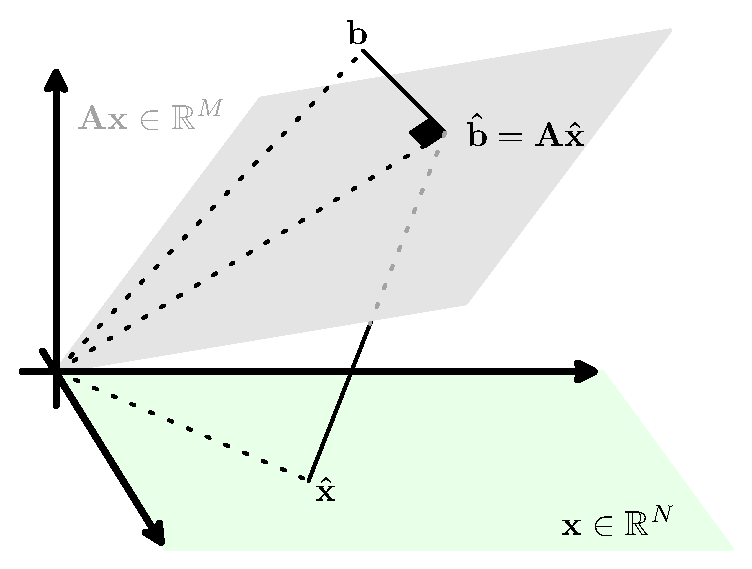
\includegraphics[width=0.9\textwidth]{chapters/minimization-fx/minimo-linear1.eps}
         \caption{Vetor $\VECTOR{d}_p$ perpendicular ao plano 
$\MATRIX{A}\VECTOR{x}$ traçado desde o ponto $\VECTOR{b}$. }
         \label{fig:coro:minAxbCAxb1:a}
     \end{figure}
\end{minipage}
\end{minipage}
\begin{minipage}{0.49\textwidth}
A partir do Teorema \ref{theo:minAxbCAxb}, 
podemos achar um vetor $\VECTOR{d}_p$ perpendicular ao plano $\MATRIX{A}\VECTOR{x}$,
partindo desde o ponto $\VECTOR{b}$, usando a seguinte equação,
\begin{equation}
\VECTOR{d}_p = \left\{\MATRIX{A}\left[ \MATRIX{A}^{\transpose}\MATRIX{A} \right]^{-1}\MATRIX{A}^{\transpose}- \MATRIX{I}\right\}\VECTOR{b},
\end{equation}
onde $I$ é uma matriz identidade.
Podemos ver graficamente o vetor $\VECTOR{d}_p$ na Figura \ref{fig:coro:minAxbCAxb1:a}.
%%
\index{Moore-Penrose!Pseudo-inversa}
\index{Pseudo-inversa!Moore-Penrose}
\begin{tcbattention}
A matriz $\left[ \MATRIX{A}^{\transpose}\MATRIX{A} \right]^{-1}\MATRIX{A}^{\transpose}$
também é chamada de pseudo inversa de Moore-Penrose da matriz $\MATRIX{A}$ \cite[pp. 290]{golub2013matrix}.
\end{tcbattention}
\end{minipage}
\end{corollary}

%%%%%%%%%%%%%%%%%%%%%%%%%%%%%%%%%%%%%%%%%%%%%%%%%%%%%%%%%%%%%%%%%%%%%%%%%%%%%%%%
\subsection{Exemplos de minimização de $||\MATRIX{A}\VECTOR{x}-\VECTOR{b}||_{\MATRIX{C}}^2$}

\begin{example}[Procurando um ponto 
$\VECTOR{\hat{x}}$ que minimize
 $||\MATRIX{A}\VECTOR{x}-\VECTOR{b}||_{\MATRIX{C}}^2$:]
\label{ex:minAxbCAxb1}
Conhecido 
um vetor coluna $\VECTOR{x}\in \mathbb{R}^2$,
as matrizes $\MATRIX{A} \in \mathbb{R}^{3\times 2}$ e $\MATRIX{C} \in \mathbb{R}^{3\times 3}_{+}$
e um ponto $\VECTOR{b} \in \mathbb{R}^{3}$,
achar o vetor $\VECTOR{x}$ que minimize $||\MATRIX{A}\VECTOR{x}-\VECTOR{b}||_{\MATRIX{C}}^2$;
sabendo que:
\begin{equation}
\VECTOR{b}=\begin{bmatrix}
1\\
1\\
1
\end{bmatrix},
\qquad 
\MATRIX{A}=\begin{bmatrix}
1 & 0\\
0 & 1\\
1 & 1
\end{bmatrix},
\qquad 
\MATRIX{C}=\begin{bmatrix}
1 & 0 & 0\\
0 & 1 & 0\\
0 & 0 & 1
\end{bmatrix}.
\end{equation}

Podemos ver a resposta a este exemplo na Solução \ref{ex:minAxbCAxb:sol1}.
\end{example}


\begin{SolutionT}[Relativa ao Exemplo \ref{ex:minAxbCAxb1}:]
\label{ex:minAxbCAxb:sol1}
Com todos estes dados e usando a Eq. (\ref{eq:minAxbCAxb1}),
obtemos a superfície $e(\VECTOR{x})$ como mostra a Figura \ref{fig:ex:minAxbCAxb:a}.
Usando a Eq. (\ref{eq:minAxbCAxb2}) sabemos que o ponto $\VECTOR{\hat{x}}=[1\quad 1]^{\transpose}$
minimiza a Eq. (\ref{eq:minAxbCAxb1}), com um $e(\VECTOR{\hat{x}})=0.12$.

Usando o Corolário \ref{coro:minAxbCAxb1}, podemos calcular o vetor $\VECTOR{d}_p=[0.2 \quad 0.2 \quad -0.2]^{\transpose}$,
como mostra o gráfico da Figura \ref{fig:ex:minAxbCAxb:b}.

\begin{figure}[h!]
     \centering
     \begin{subfigure}[b]{0.66\textwidth}
         \centering
         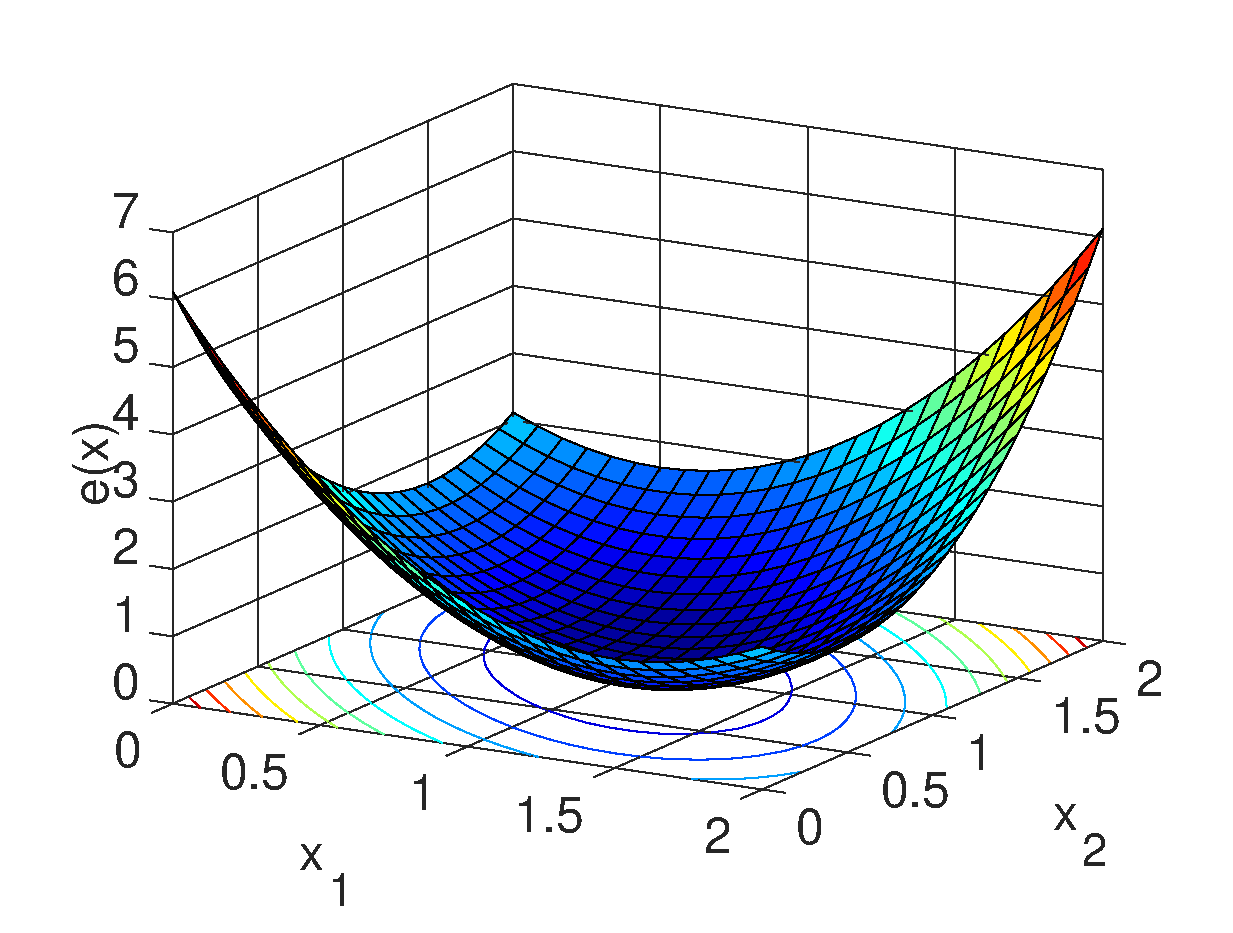
\includegraphics[width=0.98\textwidth]{chapters/minimization-fx/mfiles/ax1/surfcex.eps}
         \caption{Superfície $e(\VECTOR{x})$. }
         \label{fig:ex:minAxbCAxb:a}
     \end{subfigure}
     \hfill
     \begin{subfigure}[b]{0.32\textwidth}
         \centering
         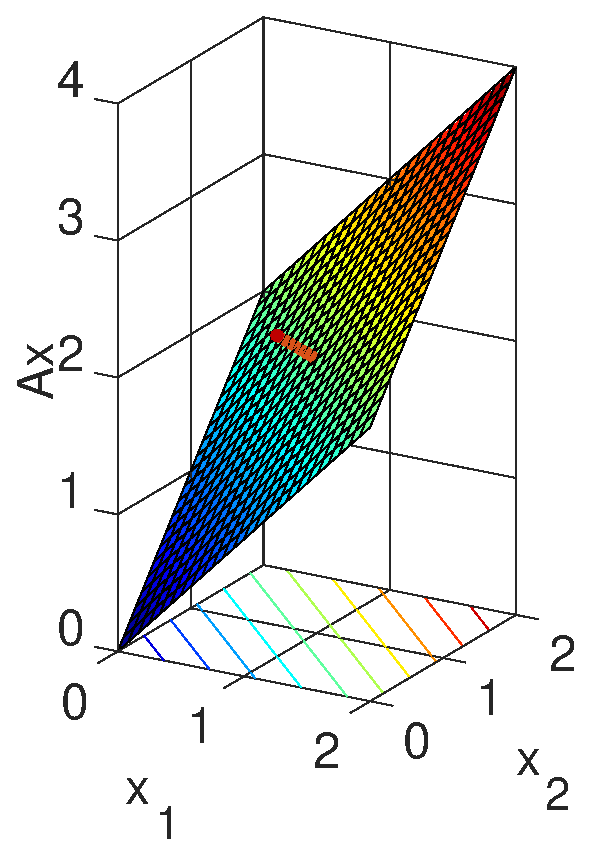
\includegraphics[width=0.98\textwidth]{chapters/minimization-fx/mfiles/ax1/surfcax.eps}
         \caption{Plano $\MATRIX{A}\VECTOR{x}$ e o vetor perpendicular $\VECTOR{b}-\MATRIX{A}\VECTOR{\hat{X}}$.}
         \label{fig:ex:minAxbCAxb:b}
     \end{subfigure}
        \caption{Resposta gráfica do Exemplo \ref{ex:minfxbCfxb3}. }
        \label{fig:ex:minAxbCAxb}
\end{figure}

\end{SolutionT}

\begin{comment}
\index{Tikhonov, Andrei Nikolaevich}
\begin{elaboracion}[title=Andrei Nikolaevich Tikhonov (1906-1993), width= 0.99\linewidth]
Matemático nascido em Rússia que trabalhou em distintas áreas como: 
topologia e análise funcional, 
equações diferenciais ordinárias e parciais, 
e sua aplicação a problemas em física matemática e matemática computacional \cite[pp. 3684]{ben2009historical}.
\end{elaboracion}
\end{comment}

\index{Tikhonov, Andrei Nikolaevich}
\index{Minimização, métodos!Regularização de Tikhonov}
\begin{tcbinformation} 
\textbf{Regularização de Tikhonov de ordem zero:} Este método foi trabalhado de forma independente
por Phillips em 1962 e por Andrei Nikolaevich Tikhonov em 1963 \cite[pp. 86]{kress2012numerical}, 
obtendo eles uma solução ótima para $\VECTOR{x}$  que minimiza $e(\VECTOR{x})$, 
\begin{equation}
e(\VECTOR{x})=||\MATRIX{A}\VECTOR{x}-\VECTOR{b}||^2+\alpha ||\VECTOR{x}||^2.
\end{equation}
Se no Teorema \ref{theo:minAxbCAxbplusalphaxqD} da  Seção \ref{sec:minAxbCAxbplusalphaxqD},
assumimos que o vetor $\VECTOR{q}=\VECTOR{0}$, a matriz $\MATRIX{C}=\MATRIX{I}$ e 
a matriz $\MATRIX{D}=\MATRIX{I}$,
então a solução representa a regularização de Tikhonov de ordem zero
\cite[pp. 94]{aster2013parameter} \cite[pp. 86]{kress2012numerical} \cite[pp. 117]{engl2000regularization}.
\end{tcbinformation} 

%%% high order tikhonov regularization \cite[pp. 103]{aster2013parameter}

\newpage

\section{Minimização de $||\MATRIX{A}\VECTOR{x}-\VECTOR{b}||_{\MATRIX{C}}^2+\alpha ||\VECTOR{x}-\VECTOR{q}||_{\MATRIX{D}}^2$}
\label{sec:minAxbCAxbplusalphaxqD}
%\index{Problema inverso!Linear}
\index{Minimização do erro quadrático!Linear}%!Função $||\MATRIX{A}\VECTOR{x}-\VECTOR{b}||_{\MATRIX{C}}^2+\alpha ||\VECTOR{x}-\VECTOR{q}||_{\MATRIX{D}}^2$}


\begin{theorem}\label{theo:minAxbCAxbplusalphaxqD}
Dados,
o escalar $\alpha \in \mathbb{R}$, 
os vetores coluna $\VECTOR{x}\in \mathbb{R}^N$, 
$\VECTOR{b}\in \mathbb{R}^M$ e
$\VECTOR{q}\in \mathbb{R}^N$,  
uma matriz $\MATRIX{A} \in \mathbb{R}^{M\times N}$, 
as matrizes diagonais $\MATRIX{C} \in \mathbb{R}^{M\times M}$ e
$\MATRIX{D} \in \mathbb{R}^{N\times N}$, e 
definida a Eq. (\ref{eq:minAxbCAxb1alphaxqD}),
\begin{equation}\label{eq:minAxbCAxb1alphaxqD}
e(\VECTOR{x})  = ||\MATRIX{A}\VECTOR{x}-\VECTOR{b}||_{\MATRIX{C}}^2 +\alpha ||\VECTOR{x}-\VECTOR{q}||_{\MATRIX{D}}^2.
\end{equation}
Se desejamos ter o valor $\VECTOR{\hat{x}}$ que minimiza o escalar $e(\VECTOR{\hat{x}})$,
devemos usar\footnote{A demostração pode ser vista na Prova \ref{proof:theo:minAxbCAxbalphaxqD}.} a Eq. (\ref{eq:minAxbCAxb2alphaxqD}),
\begin{equation}\label{eq:minAxbCAxb2alphaxqD}
\VECTOR{\hat{x}}=\left[ \MATRIX{A}^{\transpose}\MATRIX{C}\MATRIX{A} +\alpha\MATRIX{D}\right]^{-1} 
\left[ \MATRIX{A}^{\transpose}\MATRIX{C} \VECTOR{b}+\alpha\MATRIX{D}\VECTOR{q}\right].
\end{equation}
Assim, o mínimo existe só sim $\MATRIX{A}^{\transpose}\MATRIX{C}\MATRIX{A} +\alpha\MATRIX{D}$ tem inversa.
\end{theorem}



%%%%%%%%%%%%%%%%%%%%%%%%%%%%%%%%%%%%%%%%%%%%%%%%%%%%%%%%%%%%%%%%%%%%%%%%%%%%%%%%
\subsection{Exemplos de minimização de 
$||\MATRIX{A}\VECTOR{x}-\VECTOR{b}||_{\MATRIX{C}}^2+\alpha ||\VECTOR{x}-\VECTOR{q}||_{\MATRIX{D}}^2$}

\begin{example}[Procurando um ponto 
$\VECTOR{\hat{x}}$ que minimize
 $||\MATRIX{A}\VECTOR{x}-\VECTOR{b}||_{\MATRIX{C}}^2+\alpha ||\VECTOR{x}-\VECTOR{q}||_{\MATRIX{D}}^2$:]
\label{ex:minAxbCAxbplusalphaxqD1}
Conhecido 
um vetor coluna $\VECTOR{x}\in \mathbb{R}^2$,
as matrizes $\MATRIX{A} \in \mathbb{R}^{3\times 2}$, $\MATRIX{C} \in \mathbb{R}^{3\times 3}$  e $\MATRIX{D} \in \mathbb{R}^{2\times 2}$,
o escalar $\alpha \in \mathbb{R}$,
e os pontos $\VECTOR{b} \in \mathbb{R}^{3}$ e $\VECTOR{q} \in \mathbb{R}^{2}$,
achar o vetor $\VECTOR{x}$ que minimize 
$||\MATRIX{A}\VECTOR{x}-\VECTOR{b}||_{\MATRIX{C}}^2+\alpha ||\VECTOR{x}-\VECTOR{q}||_{\MATRIX{D}}^2$;
sabendo que:
\begin{equation}
\VECTOR{b}=\begin{bmatrix}
1\\
1\\
1
\end{bmatrix},
\quad 
\MATRIX{A}=\begin{bmatrix}
1 & 0\\
0 & 1\\
1 & 1
\end{bmatrix},
\quad 
\MATRIX{C}=\begin{bmatrix}
1 & 0 & 0\\
0 & 1 & 0\\
0 & 0 & 1 
\end{bmatrix},
\quad \alpha=0.5,
\quad
\VECTOR{q}=\begin{bmatrix}
0\\
0
\end{bmatrix},
\quad 
\MATRIX{D}=\begin{bmatrix}
1 & 0\\
0 & 1
\end{bmatrix}.
\end{equation}

Podemos ver a resposta a este exemplo na Solução \ref{ex:minAxbCAxbplusalphaxqD:sol1}.
\end{example}


\begin{SolutionT}[Relativa ao Exemplo \ref{ex:minAxbCAxbplusalphaxqD1}:]
\label{ex:minAxbCAxbplusalphaxqD:sol1}
Com todos estes dados e usando a Eq. (\ref{eq:minAxbCAxb1alphaxqD}),
obtemos a superficie $e(\VECTOR{x})$ como mostra a Figura \ref{fig:ex:minAxbCAxb1alphaxqD:a}.
Usando a Eq. (\ref{eq:minAxbCAxb2alphaxqD}) sabemos que o ponto $\VECTOR{\hat{x}}=[0.85714\quad 0.85714]^{\transpose}$
minimiza a Eq. (\ref{eq:minAxbCAxb1alphaxqD}), com um $e(\VECTOR{\hat{x}})=0.97714$.

\begin{figure}[h!]
         \centering
         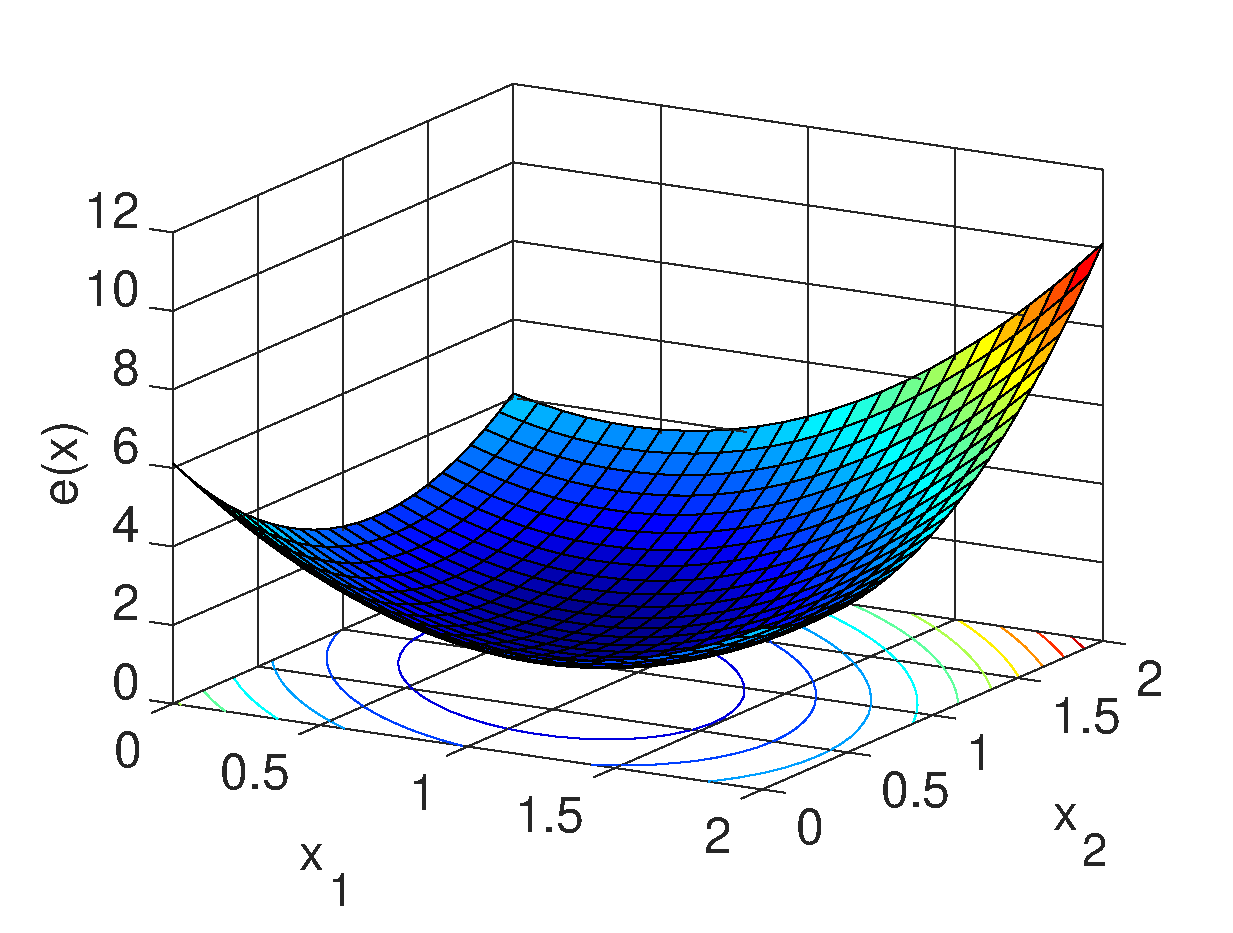
\includegraphics[width=0.6\textwidth]{chapters/minimization-fx/mfiles/axxq1/surfcex.eps}
         \caption{Superficie $e(\VECTOR{x})$. }
         \label{fig:ex:minAxbCAxb1alphaxqD:a}
\end{figure}

\end{SolutionT}


\newpage

\section{Minimização de $||\VECTOR{f}(\VECTOR{x})-\VECTOR{b}||_{\MATRIX{C}}^2$}

%\index{Minimização, métodos!Regularização de }
%\index{Problema inverso!Não linear}
\index{Minimização do erro quadrático!Não linear}%!Função $||\VECTOR{f}(\VECTOR{x})-\VECTOR{b}||_{\MATRIX{C}}^2$}

\begin{theorem}[Solução iterativa]\label{theo:minfxbCfxb}
Dados,
os vetores coluna $\VECTOR{x}\in \mathbb{R}^N$ e $\VECTOR{b}\in \mathbb{R}^M$,  
uma função $\VECTOR{f}:\mathbb{R}^{N} \rightarrow \mathbb{R}^{M}$, 
uma matriz diagonal $\MATRIX{C} \in \mathbb{R}^{M\times M}_{+}$, e 
definida a Eq. (\ref{eq:minfxbCfxb1}),
\begin{equation}\label{eq:minfxbCfxb1}
\begin{matrix}
e(\VECTOR{x}) & = & ||\VECTOR{f}(\VECTOR{x})-\VECTOR{b}||_{\MATRIX{C}}^2 \\
              & = & (\VECTOR{f}(\VECTOR{x})-\VECTOR{b})^{\transpose}\MATRIX{C}(\VECTOR{f}(\VECTOR{x})-\VECTOR{b}).
\end{matrix}
\end{equation}
Se desejamos ter o ponto $\VECTOR{x}=\VECTOR{\hat{x}}$ que minimiza o escalar $e(\VECTOR{x})$,
podemos achar este ponto usando iterativamente a Eq. (\ref{eq:minfxbCfxb2}),
onde  $\MATRIX{J}(\VECTOR{x})$ é a \hyperref[def:jacobian]{\textbf{matriz Jacobiana}}  de $\VECTOR{f}(\VECTOR{x})$.
\begin{equation}\label{eq:minfxbCfxb2}
\VECTOR{x}_{k} \leftarrow \VECTOR{x}_{k-1}-
\left[ \MATRIX{J}(\VECTOR{x}_{k-1})^{\transpose}\MATRIX{C} \MATRIX{J}(\VECTOR{x}_{k-1}) \right]^{-1}
 \MATRIX{J}(\VECTOR{x}_{k-1})^{\transpose}\MATRIX{C}\left[\VECTOR{f}(\VECTOR{x}_{k-1})-\VECTOR{b}\right];
\end{equation}



Assim, $\VECTOR{\hat{x}}$ pode ser achado 
iniciando a Eq. (\ref{eq:minfxbCfxb2}) desde um $\VECTOR{x}_{0}$ qualquer, 
ate que $\VECTOR{x}_{k}$ seja muito próximo a $\VECTOR{x}_{k-1}$,
onde se declara que $\VECTOR{\hat{x}} \approx \VECTOR{x}_{k}$,
que corresponde a um mínimo\footnote{\label{ref:minfx}A
demostração pode ser vista na Prova \ref{proof:theo:minfxbCfxb}.} de $e(\VECTOR{x})$,
sem aclarar se é local ou global.

\textbf{Considerações:}

\begin{itemize}
\item Para que tenha sentido a Eq. (\ref{eq:minfxbCfxb2}),
 e consequentemente esta possa ser usada, devemos verificar que  $\MATRIX{J}(\VECTOR{x}_{k-1})\neq \MATRIX{0}$,
pois se $\MATRIX{J}(\VECTOR{x}_{k-1})= \MATRIX{0}$ indica que existe\footref{ref:minfx} um ponto de inflexão 
(máximo, mínimo ou ponto de sela) em $e(\VECTOR{x}_{k-1})$.
\item A busca iterativa da Eq. (\ref{eq:minfxbCfxb2}) é considerada falida quando 
$\MATRIX{J}(\VECTOR{x}_{k-1})^{\transpose}$ $\MATRIX{C}$ $\MATRIX{J}(\VECTOR{x}_{k-1})$
não tem inversa.
\item A busca iterativa da Eq. (\ref{eq:minfxbCfxb2}) pode diverger quando coincide que o mínimo $\VECTOR{\hat{x}}$ procurado
tem um $\MATRIX{J}(\VECTOR{\hat{x}})\approx \MATRIX{0}$.
O erro só acontece quando $\VECTOR{x}_{k-1}$ atinge de forma ``exata'' um mínimo com $\VECTOR{f}(\VECTOR{x}_{k-1})\neq \VECTOR{b}$,
para outros valores a busca iterativa de $\VECTOR{x}_{k-1}$ avança eficazmente.
\end{itemize}

\end{theorem}
%%%%%%%%%%%%%%%%%%%%%%%%%%%%%%%%%%%%%%%%%%%%%%%%%%%%%%%%%%%%%%%%%%%%%%%%%%%%%%%%
\subsection{Exemplos de minimização de $||\VECTOR{f}(\VECTOR{x})-\VECTOR{b}||_{\MATRIX{C}}^2$}

\begin{example}[Quando existe 
$\VECTOR{\hat{x}}$ que cumpre que $\VECTOR{f}(\VECTOR{\hat{x}}) \approx \VECTOR{b}$:]
\label{ex:minfxbCfxb}
Conhecida uma função $\VECTOR{f}(\VECTOR{x}) : \mathbb{R}^{2} \rightarrow \mathbb{R}^{3}$
é um ponto $\VECTOR{b}$ do contradomínio de $\VECTOR{f}(\VECTOR{x})$,
achar o valor $\VECTOR{\hat{x}}$ que minimize $||\VECTOR{f}(\VECTOR{x})-\VECTOR{b}||_{\MATRIX{C}}^2$;
sabendo que:
\begin{equation}
\VECTOR{b}=\begin{bmatrix}
1\\
1\\
2
\end{bmatrix},
\qquad 
\VECTOR{f}(\VECTOR{x})=\begin{bmatrix}
x_1^2\\
x_2^2\\
x_1+x_2
\end{bmatrix}.
\end{equation}
Consequentemente podemos deduzir e escolher que, 
\begin{equation}\label{eq:lab:ex2fx}
\MATRIX{J}(\VECTOR{x})=\begin{bmatrix}
2 x_1 & 0\\
0 & 2 x_2\\
1 & 1
\end{bmatrix},
\qquad
\MATRIX{C}=\begin{bmatrix}
1 & 0 & 0\\
0 & 1 & 0\\
0 & 0 & 1
\end{bmatrix}.
\end{equation}
Com todos estes dados e usando a Eq. (\ref{eq:minfxbCfxb1}),
obtemos a superfície $e(\VECTOR{x})$ como mostra a Figura \ref{fig:ex:minfxbCfxb:a}.
Podemos ver as respostas a este exemplo na Solução \ref{ex:minfxbCfxb:sol1} e \ref{ex:minfxbCfxb:sol2}.
\end{example}

\begin{SolutionT}[Relativa ao Exemplo \ref{ex:minfxbCfxb}:]
\label{ex:minfxbCfxb:sol1}
Se escolhemos o ponto inicial $\VECTOR{x}_0=[0.1~0.1]^{\transpose}$ e 
usamos iterativamente a Eq. (\ref{eq:minfxbCfxb2}), obtemos os valores 
de $\VECTOR{x}_k$ e $e(\VECTOR{x}_k)$, como mostra a Tabela \ref{table:ex:minfxbCfxb},
onde se asume o final do processo iterativo quando $\VECTOR{x}_k \approx \VECTOR{x}_{k-1}$.
Assim, a aproximação iterativa conclui na resposta $\VECTOR{\hat{x}}\approx \VECTOR{x}_{4} =[1~1]^{\transpose}$,
com um erro $e(\VECTOR{\hat{x}})=5.0032~10^{-24}\approx 0$ e uma pendente\footnote{\label{ref:pendenteex} O
cálculo da pendente de $e(\VECTOR{\hat{x}})$ pode ser vista no Teorema \ref{theo:derfxbCfxb0}.}
$\frac{\partial e(\VECTOR{\hat{x}})}{\partial \VECTOR{x} }=[7.7485~10^{-12}\quad 7.7485~10^{-12}]^{\transpose}$
próxima a zero;
este processo pode ser visto de forma gráfica na Figura \ref{fig:ex:minfxbCfxb:b}.
\end{SolutionT}


\begin{table}[h!]
\centering
\begin{tabular}{|l|l|l|l|l|l|}
\hline
$k$ & 0 & 1 & 2 & 3 & 4 \\ \hline
$\VECTOR{x}_k$ & 0.10000   & 1.07941   & 1.00204   & 1.00000   & 1.00000 \\ 
~              & 0.10000   & 1.07941   & 1.00204   & 1.00000   & 1.00000 \\ \hline
$||\VECTOR{x}_k||$ & 0.14142   & 1.52652   & 1.41710   & 1.41421   & 1.41421 \\ \hline
$e(\VECTOR{x}_k)$ & 5.2002 &   7.9761e-02  & 5.0203e-05  & 2.3241e-11  & 5.0032e-24 \\ \hline
\end{tabular}
\caption{Resposta iterativa do Exemplo \ref{ex:minfxbCfxb}.}
\label{table:ex:minfxbCfxb}
\end{table}
\begin{figure}[h!]
     \centering
     \begin{subfigure}[b]{0.49\textwidth}
         \centering
         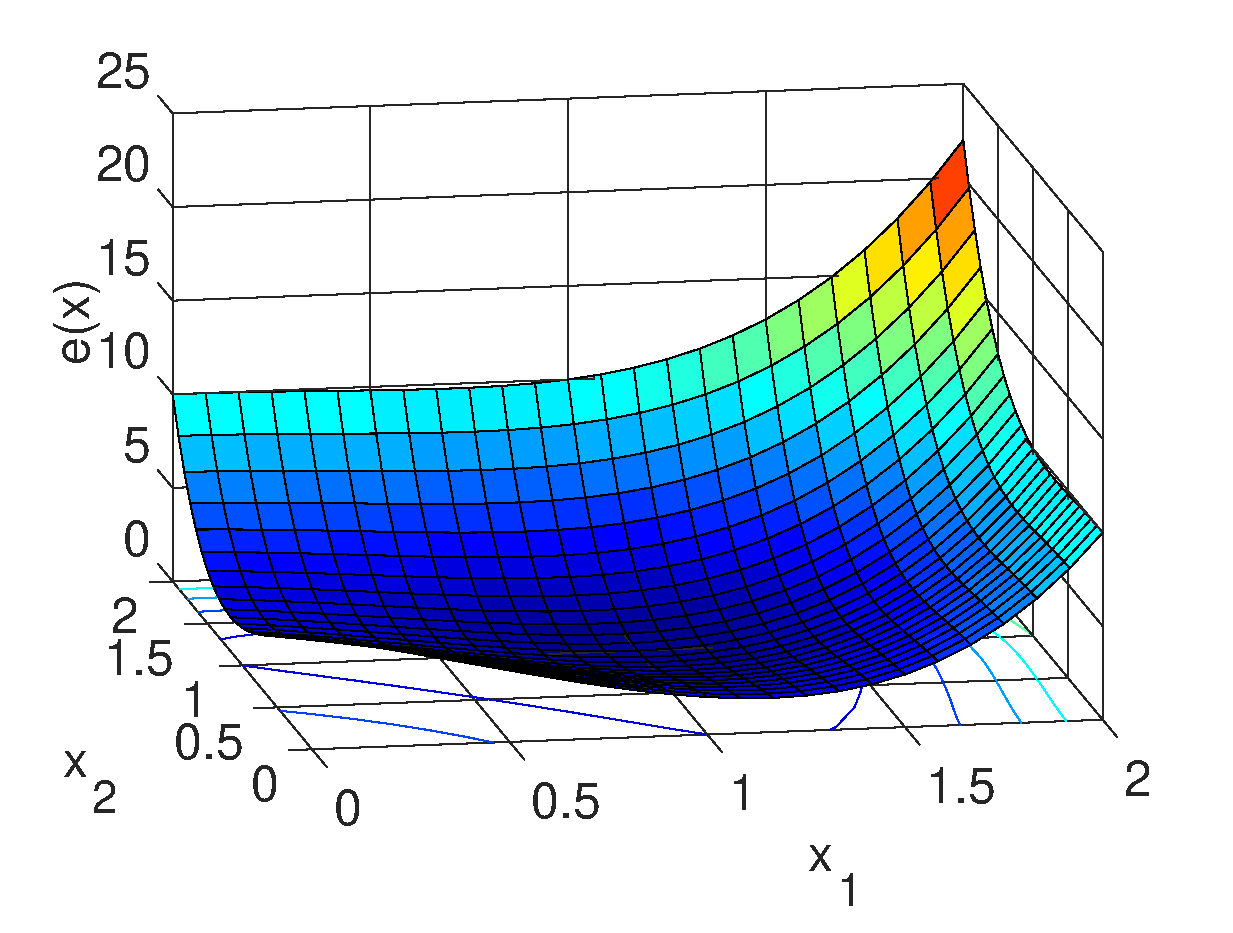
\includegraphics[width=0.98\textwidth]{chapters/minimization-fx/mfiles/fx1/surfcfx.eps}
         \caption{Superfície $e(\VECTOR{x})$. }
         \label{fig:ex:minfxbCfxb:a}
     \end{subfigure}
     \hfill
     \begin{subfigure}[b]{0.49\textwidth}
         \centering
         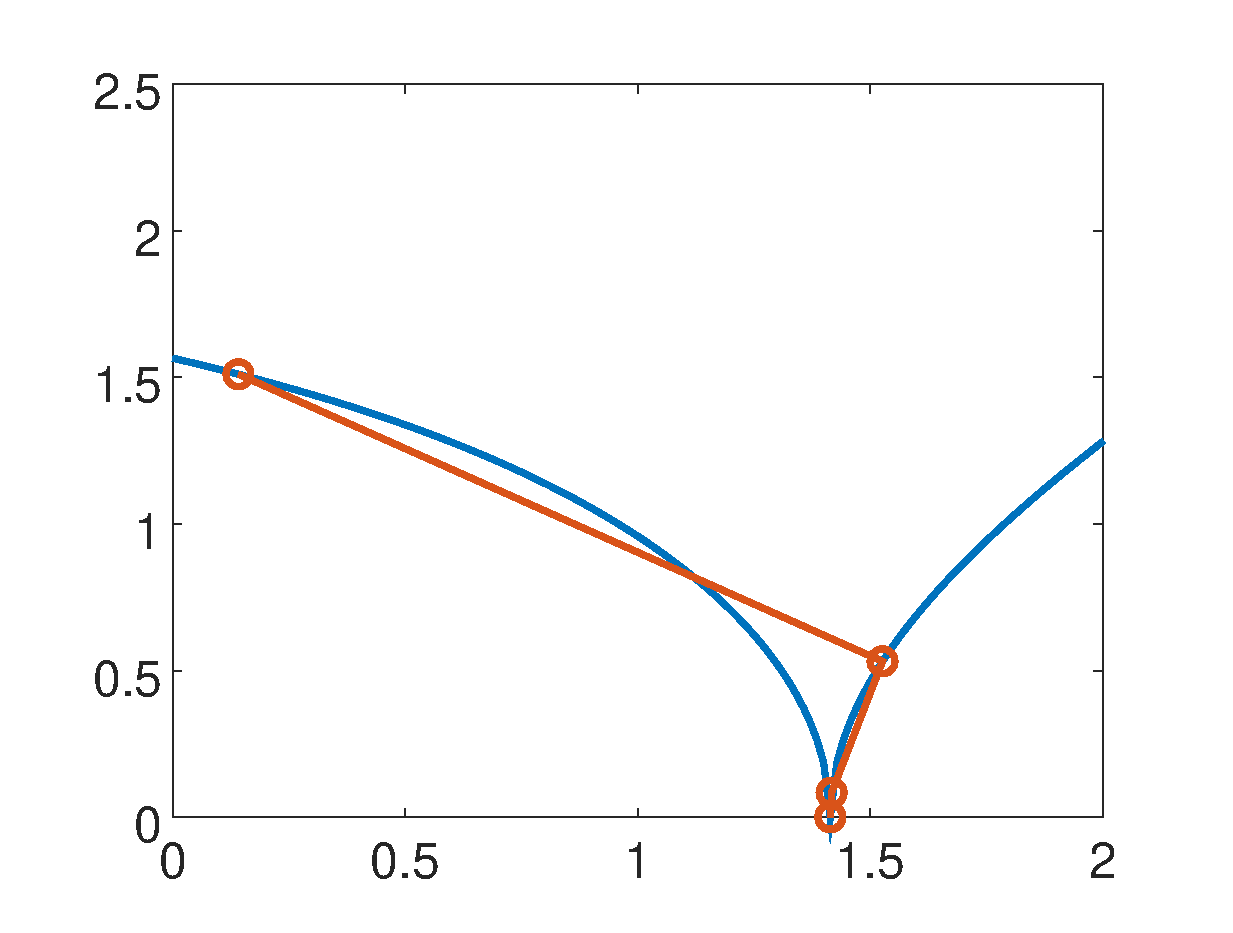
\includegraphics[width=0.98\textwidth]{chapters/minimization-fx/mfiles/fx1/plotfx.eps}
         \caption{Curva $e(\VECTOR{x})$ na direção $(1,1)$.}
         \label{fig:ex:minfxbCfxb:b}
     \end{subfigure}
        \caption{Resposta gráfica do Exemplo \ref{ex:minfxbCfxb}. }
        \label{fig:ex:minfxbCfxb}
\end{figure}


\begin{SolutionT}[Relativa ao Exemplo \ref{ex:minfxbCfxb}:]
\label{ex:minfxbCfxb:sol2}
É interessante resaltar que obteremos um erro,
se tentamos iniciar a busca iterativa desde a posição  $\VECTOR{x}_0=[0~0]^{\transpose}$
com pendente $\frac{\partial e(\VECTOR{x}_0)}{\partial \VECTOR{x} }=[-4~-4]^{\transpose}$,
pois a matriz $\MATRIX{J}(\VECTOR{x}_0)^{\transpose}\MATRIX{C} \MATRIX{J}(\VECTOR{x}_0)$
não tem inversa.
\end{SolutionT}


\begin{example}[Quando existe um
$\VECTOR{\hat{x}}$ que cumpre que $\VECTOR{f}(\VECTOR{\hat{x}}) \neq \VECTOR{b}$:]
\label{ex:minfxbCfxb2}
Conhecida uma função $\VECTOR{f}(\VECTOR{x}) : \mathbb{R}^{2} \rightarrow \mathbb{R}^{3}$
é um ponto $\VECTOR{b}$ que presumimos que existe no contradomínio $\VECTOR{f}(\VECTOR{x})$,
achar o valor $\VECTOR{\hat{x}}$ que minimize $||\VECTOR{f}(\VECTOR{x})-\VECTOR{b}||_{\MATRIX{C}}^2$;
sabendo que:
\begin{equation}
\VECTOR{b}=\begin{bmatrix}
1\\
1\\
1.5
\end{bmatrix},
\qquad 
\VECTOR{f}(\VECTOR{x})=\begin{bmatrix}
x_1^2\\
x_2^2\\
x_1+x_2
\end{bmatrix}.
\end{equation}
Com todos estes dados e usando a Eq. (\ref{eq:minfxbCfxb1}),
obtemos a superfície $e(\VECTOR{x})$ como mostra a Figura \ref{fig:ex:minfxbCfxb2:a},
na qual observamos que esta nunca atinge o valor zero.
Podemos ver uma resposta para este exemplo na Solução \ref{ex:minfxbCfxb2:sol1}.
\end{example}

\begin{SolutionT}[Relativa ao Exemplo \ref{ex:minfxbCfxb2}:]
\label{ex:minfxbCfxb2:sol1}
Este problema pode ser resolvido de forma similar ao Exemplo \ref{ex:minfxbCfxb},
usando os dados da Eq. (\ref{eq:lab:ex2fx}).
Assim, se escolhemos o ponto inicial $\VECTOR{x}_0=[0.1~0.1]^{\transpose}$ 
e usamos iterativamente a Eq. (\ref{eq:minfxbCfxb2}) obtemos os valores 
de $\VECTOR{x}_k$ e $e(\VECTOR{x}_k)$, como mostra a Tabela \ref{table:ex:minfxbCfxb2}.
A aproximação iterativa é feita ate atingir $\VECTOR{x}_k \approx \VECTOR{x}_{k-1}$,
onde concluimos que a resposta é $\VECTOR{\hat{x}}\approx \VECTOR{x}_5 =[0.90856\quad 0.90856]^{\transpose}$
com um erro $e(\VECTOR{\hat{x}})=0.16148$; é dizer, não existe $\VECTOR{f}(\VECTOR{\hat{x}})$
que seja igual a $\VECTOR{b}$, só podemos achar um vetor $\VECTOR{\hat{x}}$ 
que provoque um valor com mínimo erro, com pendente 
$\frac{\partial e(\VECTOR{\hat{x}})}{\partial \VECTOR{x} }=[-9.7332~10^{-6}\quad -9.7332~{10}^{-6}]^{\transpose}$
e um
\begin{equation}
\MATRIX{J}(\VECTOR{\hat{x}})=
\begin{bmatrix}
1.81712 & 0.0\\ 
0.0     & 1.81712\\
1       & 1
\end{bmatrix}.
\end{equation}
Todo este processo pode ser visto de forma gráfica na Figura \ref{fig:ex:minfxbCfxb2:b}.
\end{SolutionT}

\begin{table}[h!]
\centering
\begin{tabular}{|l|l|l|l|l|l|l|}
\hline
$k$ & 0 & 1 & 2 & 3 & 4 & 5 \\ \hline
$\VECTOR{x}_k$ & 0.10000   & 0.83431   & 0.90507   & 0.90833   & 0.90855   & 0.90856 \\ 
~              & 0.10000   & 0.83431   & 0.90507   & 0.90833   & 0.90855   & 0.90856 \\ \hline
$||\VECTOR{x}_k||$ & 0.14142   & 1.17989   & 1.27996   & 1.28457   & 1.28488   & 1.28490 \\ \hline
$e(\VECTOR{x}_k)$ & 3.65020  & 0.21317  & 0.16160  & 0.16148  & 0.16148  & 0.16148 \\ \hline
\end{tabular}
\caption{Resposta iterativa do Exemplo \ref{ex:minfxbCfxb2}.}
\label{table:ex:minfxbCfxb2}
\end{table}
\begin{figure}[h!]
     \centering
     \begin{subfigure}[b]{0.49\textwidth}
         \centering
         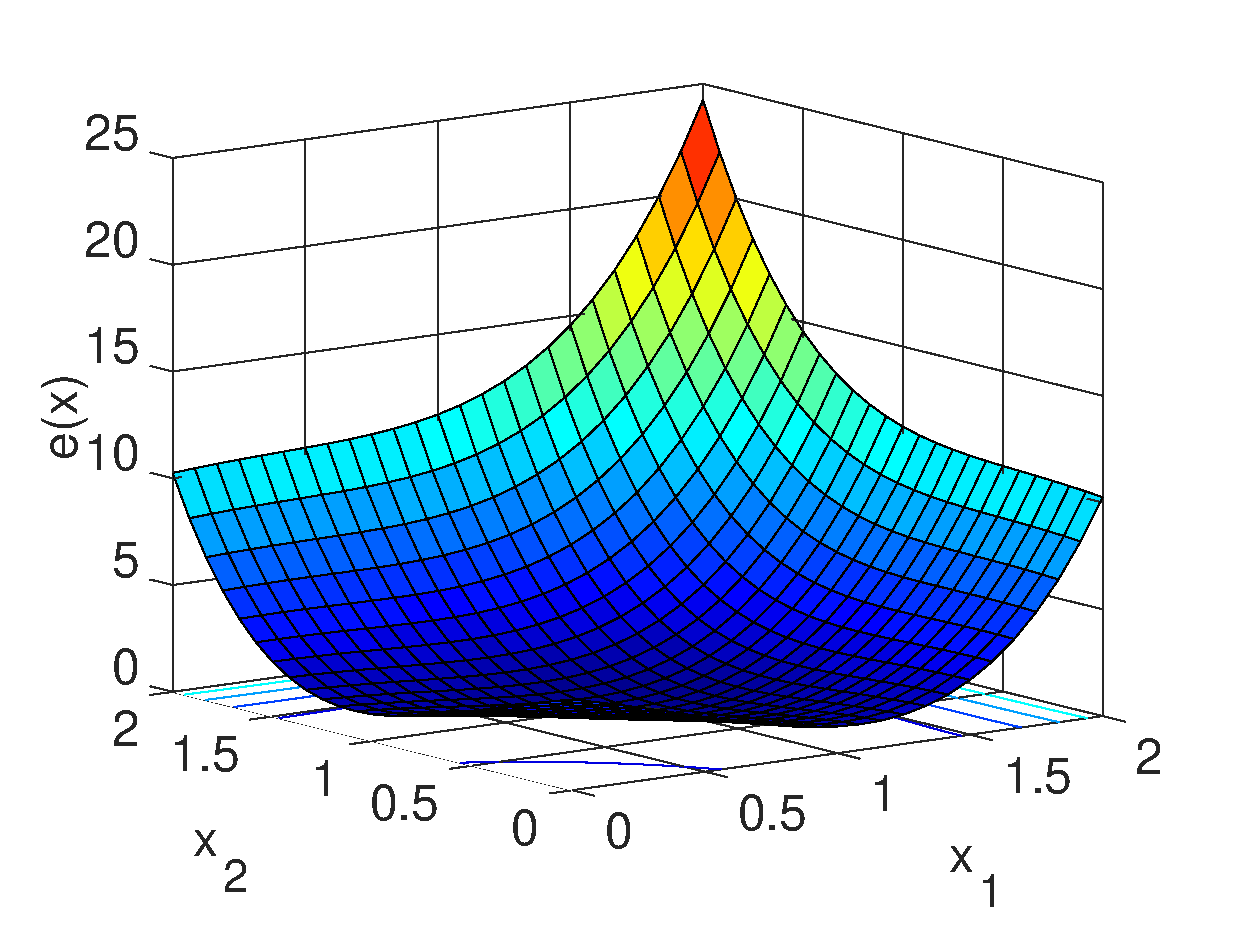
\includegraphics[width=0.98\textwidth]{chapters/minimization-fx/mfiles/fx1/surfcfx2.eps}
         \caption{Superfície $e(\VECTOR{x})$. }
         \label{fig:ex:minfxbCfxb2:a}
     \end{subfigure}
     \hfill
     \begin{subfigure}[b]{0.49\textwidth}
         \centering
         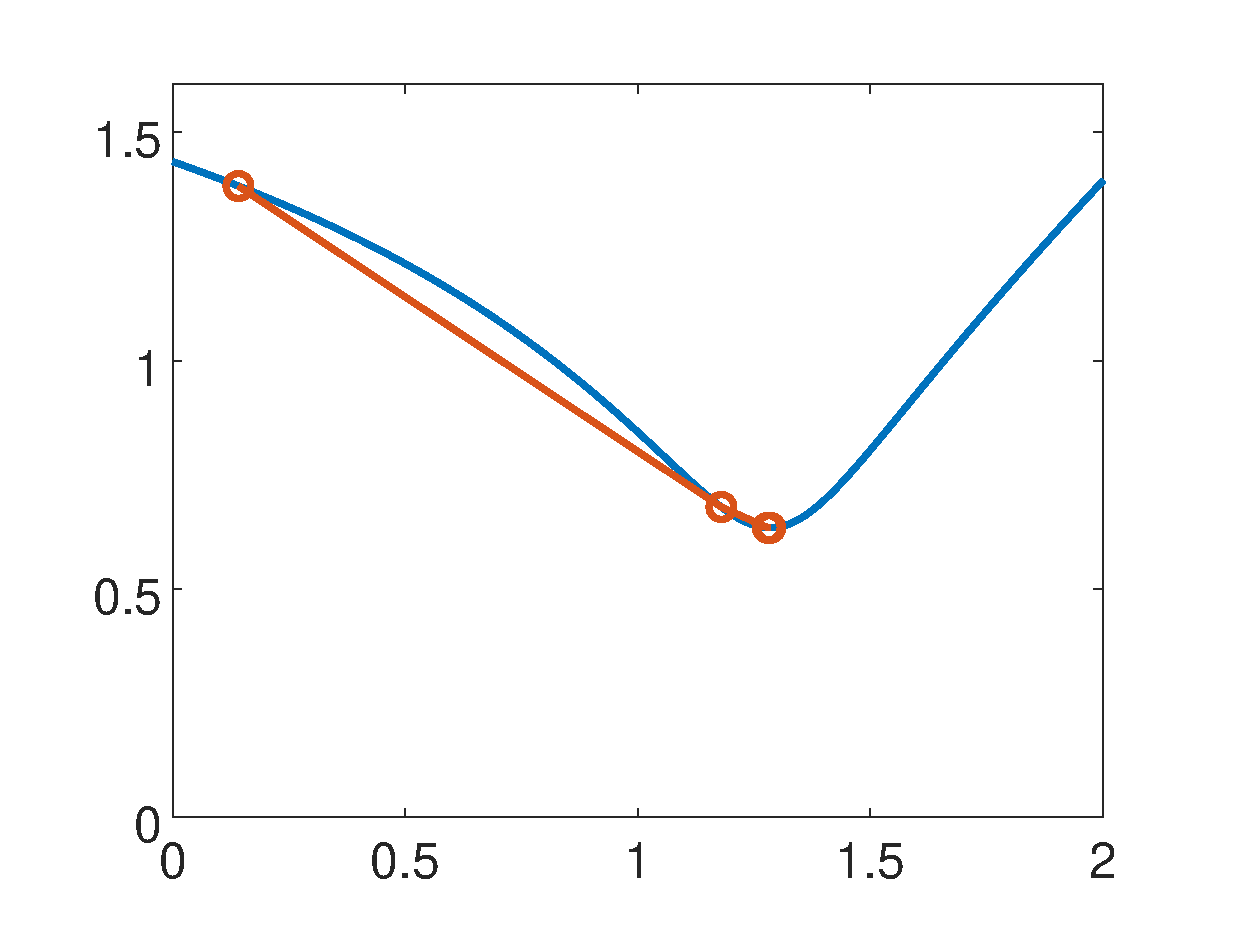
\includegraphics[width=0.98\textwidth]{chapters/minimization-fx/mfiles/fx1/plotfx2.eps}
         \caption{Curva $e(\VECTOR{x})$ na direção $(1,1)$.}
         \label{fig:ex:minfxbCfxb2:b}
     \end{subfigure}
        \caption{Resposta gráfica do Exemplo \ref{ex:minfxbCfxb2}. }
        \label{fig:ex:minfxbCfxb2}
\end{figure}


\begin{example}[Quando existem muitos mínimos locais e um
$\VECTOR{\hat{x}}$ que cumpre que $\VECTOR{f}(\VECTOR{\hat{x}}) \approx \VECTOR{b}$:]
\label{ex:minfxbCfxb3}
Conhecida uma função $\VECTOR{f}(\VECTOR{x}) : \mathbb{R}^{2} \rightarrow \mathbb{R}^{3}$
é um ponto $\VECTOR{b}$ do contradomínio de $\VECTOR{f}(\VECTOR{x})$,
achar o valor $\VECTOR{\hat{x}}$ que minimize $||\VECTOR{f}(\VECTOR{x})-\VECTOR{b}||_{\MATRIX{C}}^2$;
sabendo que:
\begin{equation}
\VECTOR{b}=\begin{bmatrix}
1\\
1\\
2
\end{bmatrix},
\qquad 
\VECTOR{f}(\VECTOR{x})=\begin{bmatrix}
sin(\frac{x_1 5 \pi}{2})\\
sin(\frac{x_2 5 \pi}{2})\\
x_1+x_2
\end{bmatrix}.
\end{equation}
Consequentemente podemos deduzir e escolher que, 
\begin{equation}\label{eq:lab:ex2fx3}
\MATRIX{J}(\VECTOR{x})=\begin{bmatrix}
\frac{5 \pi}{2}cos(\frac{x_1 5 \pi}{2}) & 0\\
0 & \frac{5 \pi}{2}cos(\frac{x_2 5 \pi}{2}) \\
1 & 1
\end{bmatrix},
\qquad
\MATRIX{C}=\begin{bmatrix}
1 & 0 & 0\\
0 & 1 & 0\\
0 & 0 & 1
\end{bmatrix}.
\end{equation}
Com todos estes dados e usando a Eq. (\ref{eq:minfxbCfxb1}),
obtemos a superfície $e(\VECTOR{x})$ como mostra a Figura \ref{fig:ex:minfxbCfxb3:a}.
Podemos ver as respostas a este exemplo na Solução \ref{ex:minfxbCfxb3:sol1} e \ref{ex:minfxbCfxb3:sol2}.
\end{example}

\begin{SolutionT}[Relativa ao Exemplo \ref{ex:minfxbCfxb3}:]
\label{ex:minfxbCfxb3:sol1}
Se escolhemos o ponto inicial $\VECTOR{x}_0=[\frac{11.0999}{5}$ $\frac{11.0999}{5}]^{\transpose}$,
com pendente\footnote{O cálculo da
pendente de $e(\VECTOR{\hat{x}})$ pode ser visto no Teorema \ref{theo:derfxbCfxb0}.} 
$\frac{\partial e(\VECTOR{x}_0)}{\partial \VECTOR{x} }=[4.2318~10^{-4}\quad 4.2318~10^{-4}]^{\transpose}$ e 
usamos iterativamente a Eq. (\ref{eq:minfxbCfxb2}), obtemos os valores 
de $\VECTOR{x}_k$ e $e(\VECTOR{x}_k)$, como mostra a Tabela \ref{table:ex:minfxbCfxb3},
onde se asume o final do processo iterativo quando $\VECTOR{x}_k \approx \VECTOR{x}_{k-1}$.
Assim, a aproximação iterativa conclui na resposta $\VECTOR{\hat{x}}\approx \VECTOR{x}_{7} =[1.7076\quad 1.7076]^{\transpose}$
com um erro $e(\VECTOR{\hat{x}})=2.1298$, uma pendente
$\frac{\partial e(\VECTOR{\hat{x}})}{\partial \VECTOR{x} }=[0.20251\quad 0.20251]^{\transpose}$
e um
\begin{equation}
\MATRIX{J}(\VECTOR{\hat{x}})=
\begin{bmatrix}
5.21306 & 0.0\\ 
0.0     & 5.21306\\
1       & 1
\end{bmatrix};
\end{equation}
este processo pode ser visto de forma gráfica na Figura \ref{fig:ex:minfxbCfxb3:b}.

É interesante resaltar que o ponto $\VECTOR{x}_0$ é muito próximo a um máximo local de 
$e(\VECTOR{x})$, e o uso iterativo da Eq. (\ref{eq:minfxbCfxb2}) 
provoca o afastamento deste ponto, mesmo que a princípio os passos sejam pequenos;
por outro lado, a busca iterativa converge e finaliza em $\VECTOR{x}_7$ um mínimo local 
de $e(\VECTOR{x})$.

\end{SolutionT}

\begin{table}[h!]
\centering
\begin{tabular}{|l|l|l|l|l|l|l|l|l|}
\hline
$k$ & 0 & 1 & 2 & 3 & 4 & 5 & 6 & 7\\ \hline
$\VECTOR{x}_k$ & 2.2200   & 2.2199   & 2.2178   & 2.1385   & 1.5400   & 1.7184   & 1.6974   & 1.7076 \\ 
~              & 2.2200   & 2.2199   & 2.2178   & 2.1385   & 1.5400   & 1.7184   & 1.6974   & 1.7076 \\ \hline
$||\VECTOR{x}_k||$ & 3.1396   & 3.1394   & 3.1364   & 3.0243   & 2.1779   & 2.4302   & 2.4005   & 2.4149 \\ \hline
$e(\VECTOR{x}_k)$ & 13.8554  & 13.8554  & 13.8543  & 12.2971   & 5.3932   & 2.1432   & 2.1346   & 2.1298 \\ \hline
\end{tabular}
\caption{Resposta iterativa do Exemplo \ref{ex:minfxbCfxb3}.}
\label{table:ex:minfxbCfxb3}
\end{table}
\begin{figure}[h!]
     \centering
     \begin{subfigure}[b]{0.49\textwidth}
         \centering
         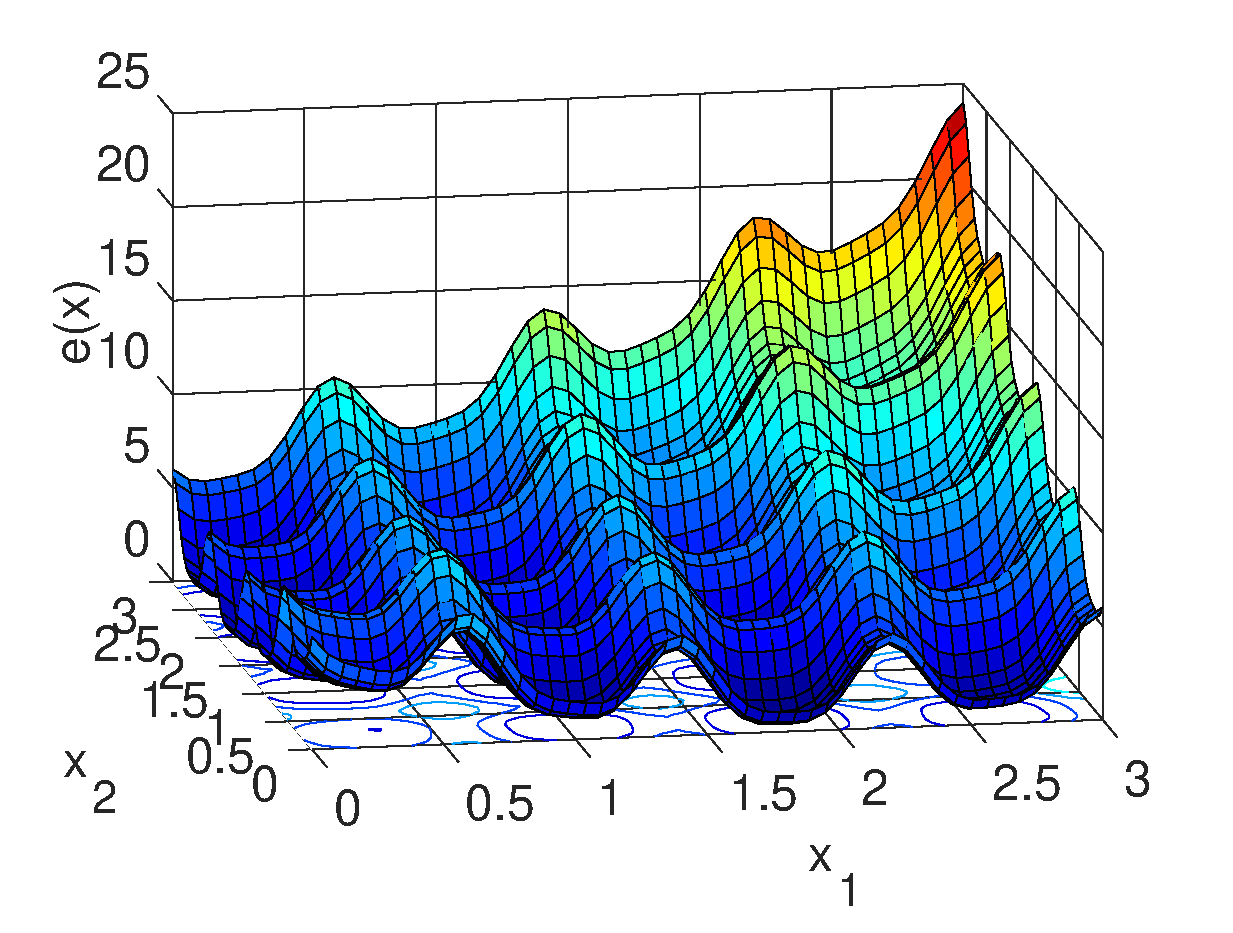
\includegraphics[width=0.98\textwidth]{chapters/minimization-fx/mfiles/fx3/surfcfx3.eps}
         \caption{Superfície $e(\VECTOR{x})$. }
         \label{fig:ex:minfxbCfxb3:a}
     \end{subfigure}
     \hfill
     \begin{subfigure}[b]{0.49\textwidth}
         \centering
         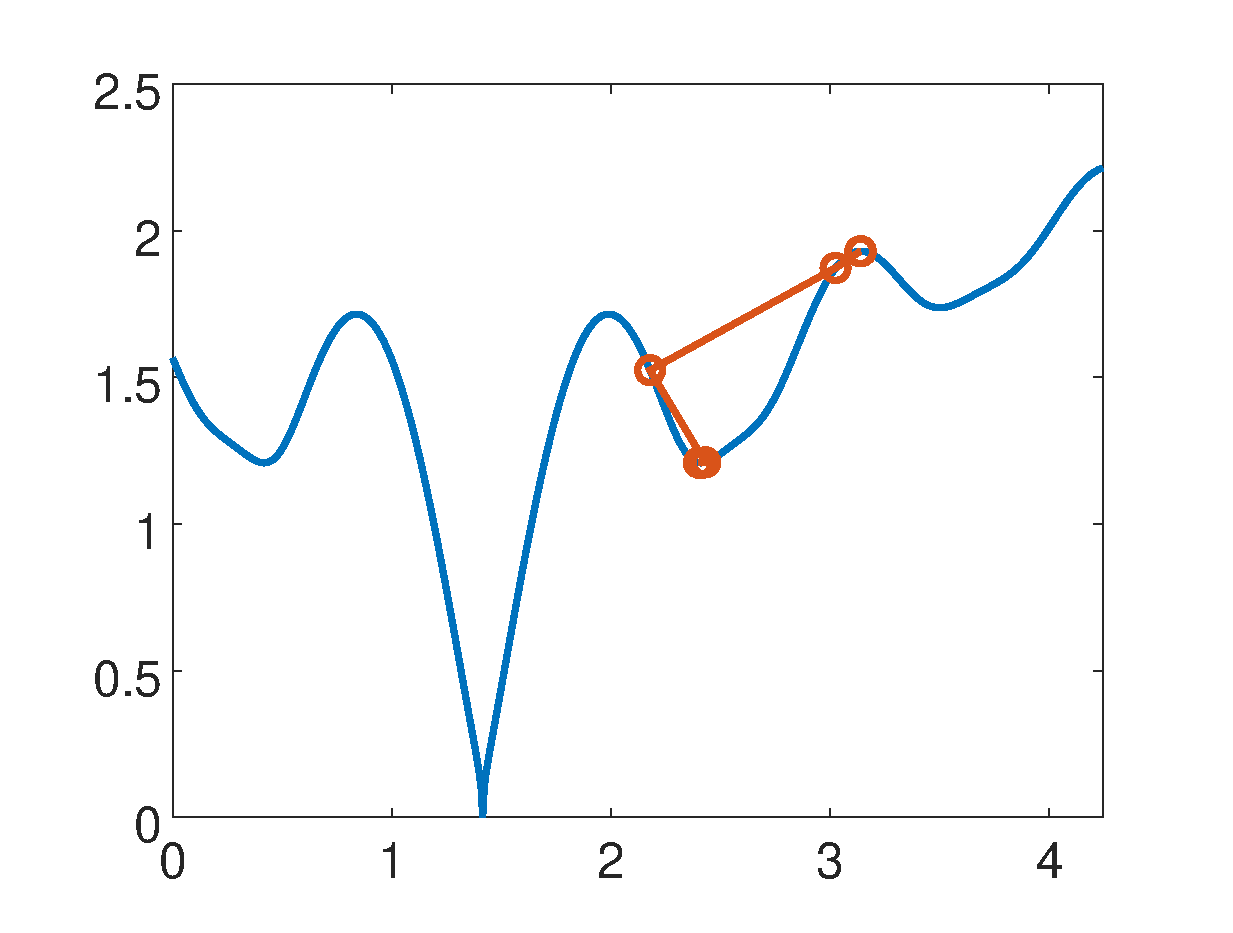
\includegraphics[width=0.98\textwidth]{chapters/minimization-fx/mfiles/fx3/plotfx3.eps}
         \caption{Curva $e(\VECTOR{x})$ na direção $(1,1)$.}
         \label{fig:ex:minfxbCfxb3:b}
     \end{subfigure}
        \caption{Resposta gráfica do Exemplo \ref{ex:minfxbCfxb3}. }
        \label{fig:ex:minfxbCfxb3}
\end{figure}

\begin{SolutionT}[Relativa ao Exemplo \ref{ex:minfxbCfxb3}:]
\label{ex:minfxbCfxb3:sol2}
Se escolhemos o ponto inicial $\VECTOR{x}_0=[\frac{7.032993}{5}$ $\frac{7.032993}{5}]^{\transpose}$,
com pendente\footnote{O cálculo da
pendente de $e(\VECTOR{\hat{x}})$ pode ser visto no Teorema \ref{theo:derfxbCfxb0}.} 
$\frac{\partial e(\VECTOR{x}_0)}{\partial \VECTOR{x} }=[7.6342~10^{-5}\quad 7.6342~10^{-5}]^{\transpose}$ e 
usamos iterativamente a Eq. (\ref{eq:minfxbCfxb2}), obtemos os valores 
de $\VECTOR{x}_k$ e $e(\VECTOR{x}_k)$, como mostra a Tabela \ref{table:ex:minfxbCfxb4},
onde se asume o final do processo iterativo quando $\VECTOR{x}_k \approx \VECTOR{x}_{k-1}$.
Assim, a aproximação iterativa conclui na resposta $\VECTOR{\hat{x}}\approx \VECTOR{x}_{7} =[0.99056\quad 0.99056]^{\transpose}$,
com um erro $e(\VECTOR{\hat{x}})=3.7152~10^{-4}$, uma pendente
$\frac{\partial e(\VECTOR{\hat{x}})}{\partial \VECTOR{x} }=[-0.040955\quad -0.040955]^{\transpose}$
e um
\begin{equation}
\MATRIX{J}(\VECTOR{\hat{x}})=
\begin{bmatrix}
0.58175 & 0.0\\ 
0.0     & 0.58175\\
1       & 1
\end{bmatrix};
\end{equation}
este processo pode ser visto de forma gráfica na Figura \ref{fig:ex:minfxbCfxb4:b}.

De forma similar ao Exemplo \ref{ex:minfxbCfxb3:sol1}, observamos 
que o ponto $\VECTOR{x}_0$ é muito próximo a um máximo local de 
$e(\VECTOR{x})$, e o uso iterativo da Eq. (\ref{eq:minfxbCfxb2}) 
provoca o afastamento deste ponto, mesmo que a princípio os passos sejam pequenos;
por outro lado, a busca iterativa converge e finaliza em $\VECTOR{x}_7$ um mínimo global
de $e(\VECTOR{x})$.
\end{SolutionT}


\begin{table}[h!]
\centering
\begin{tabular}{|l|l|l|l|l|l|l|l|l|}
\hline
$k$ & 0 & 1 & 2 & 3 & 4 & 5 & 6 & 7\\ \hline
$\VECTOR{x}_k$ & 1.40660   & 1.40658   & 1.40558   & 1.34728   & 0.78432   & 0.93066   & 0.96985   & 0.99056 \\ 
~              & 1.40660   & 1.40658   & 1.40558   & 1.34728   & 0.78432   & 0.93066   & 0.96985   & 0.99056 \\ \hline
$||\VECTOR{x}_k||$ & 1.9892   & 1.9892   & 1.9878   & 1.9053   & 1.1092   & 1.3162   & 1.3716   & 1.4009 \\ \hline
$e(\VECTOR{x}_k)$ & 8.6506  & 8.6506  & 8.6503  & 7.8206  & 2.7076  & 6.109e-2 &  5.192e-3  & 3.715e-4 \\ \hline
\end{tabular}
\caption{Resposta iterativa do Exemplo \ref{ex:minfxbCfxb3}.}
\label{table:ex:minfxbCfxb4}
\end{table}

     \begin{figure}[!h]
         \centering
         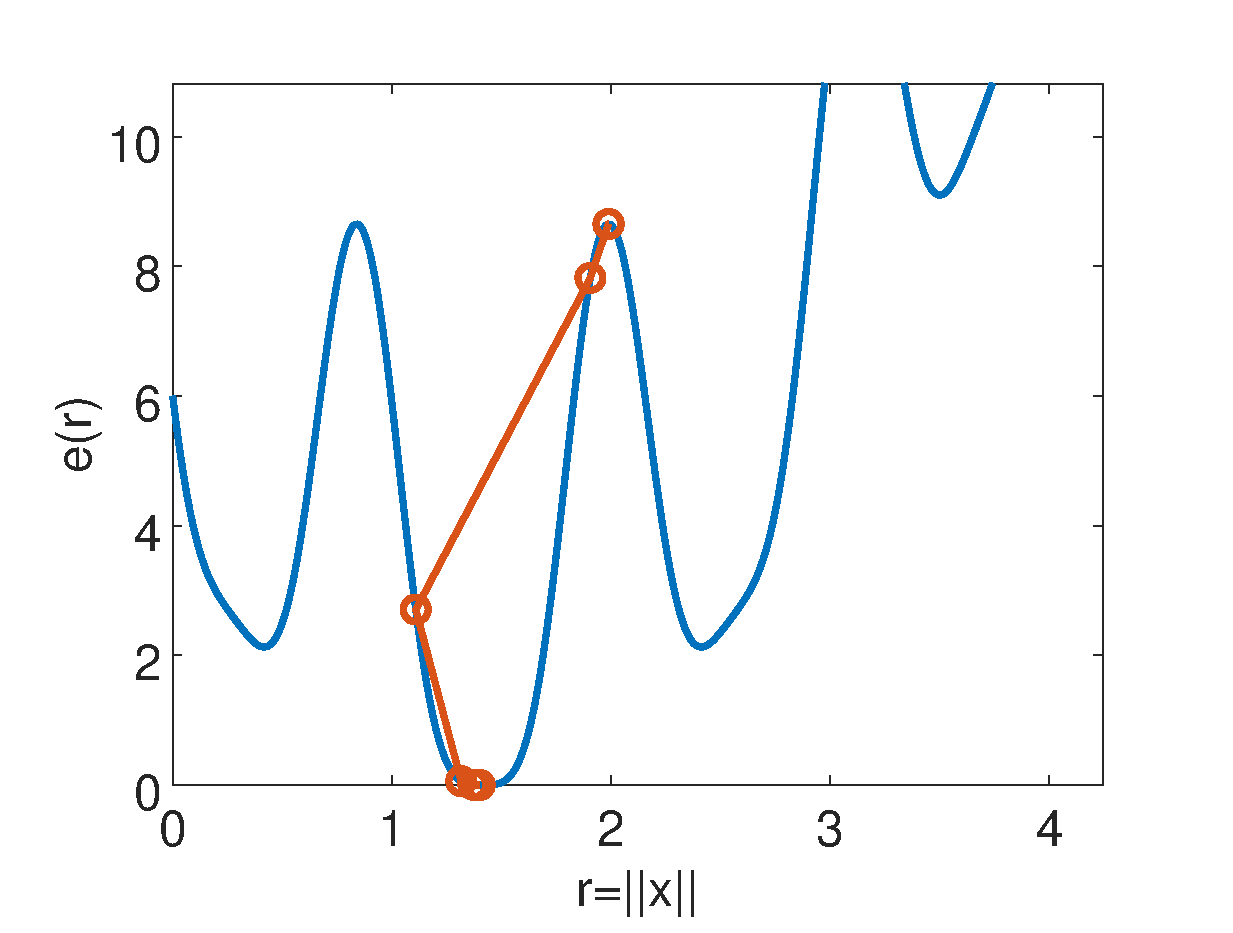
\includegraphics[width=0.5\textwidth]{chapters/minimization-fx/mfiles/fx3/plotfx4.eps}
         \caption{Curva $e(\VECTOR{x})$ na direção $(1,1)$.}
         \label{fig:ex:minfxbCfxb4:b}
     \end{figure}



\newpage

\section{Minimização de $||\VECTOR{f}(\VECTOR{x})-\VECTOR{b}||_{\MATRIX{C}}^2+\alpha||\VECTOR{x}-\VECTOR{q}||_{\MATRIX{D}}^2$}


%\index{Minimização, métodos!Regularização de }
%\index{Problema inverso!Não linear}
\index{Minimização do erro quadrático!Não linear}%!Função $||\VECTOR{f}(\VECTOR{x})-\VECTOR{b}||_{\MATRIX{C}}^2+\alpha||\VECTOR{x}-\VECTOR{q}||_{\MATRIX{D}}^2$}

\begin{theorem}[Solução iterativa:]\label{theo:minfxbCfxbaxqaxq}
Dados,
o escalar $\alpha \in \mathbb{R}_{+}$,
os vetores coluna $\VECTOR{x}\in \mathbb{R}^N$, $\VECTOR{b}\in \mathbb{R}^M$ e $\VECTOR{q}\in \mathbb{R}^N$,  
uma função $\VECTOR{f}:\mathbb{R}^{N} \rightarrow \mathbb{R}^{M}$, 
as matrizes diagonais $\MATRIX{C} \in \mathbb{R}^{M\times M}_{+}$ e $\MATRIX{D} \in \mathbb{R}^{N\times N}_{+}$, e 
definida a Eq. (\ref{eq:minfxbCfxbaxqaxq1}),
\begin{align}\label{eq:minfxbCfxbaxqaxq1}
e(\VECTOR{x}) &=||\VECTOR{f}(\VECTOR{x})-\VECTOR{b}||_{\MATRIX{C}}^2+\alpha||\VECTOR{x}-\VECTOR{q}||_{\MATRIX{D}}^2\\
              & = (\VECTOR{f}(\VECTOR{x})-\VECTOR{b})^{\transpose}\MATRIX{C}(\VECTOR{f}(\VECTOR{x})-\VECTOR{b})+\alpha(\VECTOR{x}-\VECTOR{q})^{\transpose}\MATRIX{D}(\VECTOR{x}-\VECTOR{q}).
\end{align}
Se desejamos ter o ponto $\VECTOR{x}=\VECTOR{\hat{x}}$ que minimiza o escalar $e(\VECTOR{x})$,
podemos achar este ponto usando iterativamente a Eq. (\ref{eq:minfxbCfxbaxqaxq2}),
onde  $\MATRIX{J}(\VECTOR{x})$ é a \hyperref[def:jacobian]{\textbf{matriz Jacobiana}}  de $\VECTOR{f}(\VECTOR{x})$,
\begin{equation}\label{eq:minfxbCfxbaxqaxq2}
\VECTOR{x}_{k}\leftarrow \VECTOR{x}_{k-1}-
\left[ \MATRIX{J}(\VECTOR{x}_{k-1})^{\transpose}\MATRIX{C} \MATRIX{J}(\VECTOR{x}_{k-1}) +\alpha\MATRIX{D} \right]^{-1}
 \left\{\MATRIX{J}(\VECTOR{x}_{k-1})^{\transpose}\MATRIX{C}\left[\VECTOR{f}(\VECTOR{x}_{k-1})-\VECTOR{b}\right]+\alpha\MATRIX{D}\left[\VECTOR{x}_{k-1}-\VECTOR{q}\right]\right\},
\end{equation}

Assim, $\VECTOR{\hat{x}}$ pode ser achado 
iniciando a Eq. (\ref{eq:minfxbCfxbaxqaxq2}) desde um $\VECTOR{x}_{0}$ qualquer, 
ate que $\VECTOR{x}_{k}$ seja muito próximo a $\VECTOR{x}_{k-1}$,
onde se declara que $\VECTOR{\hat{x}} \approx \VECTOR{x}_{k}$,
que corresponde a um mínimo\footnote{\label{ref:minfxxq}A
demostração pode ser vista na Prova \ref{proof:theo:minfxbCfxbaxqd}.} de $e(\VECTOR{x})$,
sem aclarar se é local ou global.


\textbf{Considerações:}

\begin{itemize}
\item É interessante verificar na Eq. (\ref{eq:minfxbCfxbaxqaxq2}) 
se  $\MATRIX{J}(\VECTOR{x}_{k-1}=\VECTOR{q}) = \MATRIX{0}$,
pois indica que existe\footref{ref:minfxxq} um ponto de inflexão 
(máximo, mínimo ou ponto de sela) em $e(\VECTOR{x}_{k-1}=\VECTOR{q})$;
consequentemente poderíamos ter achado um mínimo\footnote{\label{foot:labq}É 
interessante verificar o ponto $\VECTOR{q}$, uma vez só, 
antes de iniciar a busca iterativa.}.
\item A busca iterativa da Eq. (\ref{eq:minfxbCfxbaxqaxq2}) falha quando 
$\MATRIX{J}(\VECTOR{x}_{k-1})^{\transpose}\MATRIX{C} \MATRIX{J}(\VECTOR{x}_{k-1}) +\alpha\MATRIX{D}$
não tem inversa.
\end{itemize}

\end{theorem} 

\begin{tcbattention}
\begin{itemize}
\item O Teorema \ref{theo:minfxbCfxbaxqaxq} pode ser usado para achar o vetor $\VECTOR{x}$
que minimize $e(\VECTOR{x})=||\VECTOR{f}(\VECTOR{x})-\VECTOR{b}||_{\MATRIX{C}}^2+\alpha||\VECTOR{x}-\VECTOR{q}||_{\MATRIX{D}}^2$,
quando sabemos que o vetor $\VECTOR{x}$ que minimiza $||\VECTOR{f}(\VECTOR{x})-\VECTOR{b}||_{\MATRIX{C}}^2$ 
está perto do ponto $\VECTOR{q}$.
\item No Teorema \ref{theo:minfxbCfxbaxqaxq} o vetor $\VECTOR{x}$ que minimiza $e(\VECTOR{x})$, 
não necessariamente minimiza  $||\VECTOR{f}(\VECTOR{x})-\VECTOR{b}||_{\MATRIX{C}}^2$.
\end{itemize}
\end{tcbattention}

%%%%%%%%%%%%%%%%%%%%%%%%%%%%%%%%%%%%%%%%%%%%%%%%%%%%%%%%%%%%%%%%%%%%%%%%%%%%%%%%
\subsection{Exemplos de minimização de 
$||\VECTOR{f}(\VECTOR{x})-\VECTOR{b}||_{\MATRIX{C}}^2+\alpha||\VECTOR{x}-\VECTOR{q}||_{\MATRIX{D}}^2$}


\begin{example}[Quando existem muitos mínimos locais e um
$\VECTOR{\hat{x}}$ que cumpre que $\VECTOR{f}(\VECTOR{\hat{x}}) \approx \VECTOR{b}$:]
\label{ex:minfxbCfxbaxqaxq1}
Conhecida um escalar $\alpha$, uma função $\VECTOR{f}(\VECTOR{x}) : \mathbb{R}^{2} \rightarrow \mathbb{R}^{3}$,
um ponto $\VECTOR{q}$
e outro ponto $\VECTOR{b}$, no domínio e no contradomínio de $\VECTOR{f}(\VECTOR{x})$, respetivamente;
achar o valor $\VECTOR{\hat{x}}$ que minimize 
$||\VECTOR{f}(\VECTOR{x})-\VECTOR{b}||_{\MATRIX{C}}^2+\alpha||\VECTOR{x}-\VECTOR{q}||_{\MATRIX{D}}^2$;
sabendo que:
\begin{equation}
\VECTOR{b}=\begin{bmatrix}
1\\
1\\
2
\end{bmatrix},
\qquad 
\VECTOR{f}(\VECTOR{x})=\begin{bmatrix}
sin(\frac{x_1 5 \pi}{2})\\
sin(\frac{x_2 5 \pi}{2})\\
x_1+x_2
\end{bmatrix},
\qquad
\alpha=0.1,
\qquad
\VECTOR{q}=\begin{bmatrix}
0\\
0\\
0
\end{bmatrix}.
\end{equation}
Com esta informação podemos calcular o jacobiano $\MATRIX{J}(\VECTOR{x})$ de $\VECTOR{f}(\VECTOR{x})$,
 e escolher as matrizes $\MATRIX{C} \in \mathbb{R}^{3\times 3}_{+}$ e $\MATRIX{D} \in \mathbb{R}^{2\times 2}_{+}$, 
com elementos iguais à  matriz identidade. 
Assim, usando a Eq. (\ref{eq:minfxbCfxbaxqaxq1}),
obtemos a superfície $e(\VECTOR{x})$ como mostra a Figura \ref{fig:ex:minfxbCfxbaxqaxq3:a}.
Podemos ver duas respostas a este exemplo na Solução \ref{ex:minfxbCfxbaxqaxq3:sol1} e \ref{ex:minfxbCfxbaxqaxq3:sol2}.
\end{example}

\begin{SolutionT}[Relativa ao Exemplo \ref{ex:minfxbCfxbaxqaxq1}:]
\label{ex:minfxbCfxbaxqaxq3:sol1}
Se escolhemos o ponto inicial $\VECTOR{x}_0=[2\quad 2]^{\transpose}$,
com pendente\footnote{O cálculo da
pendente de $e(\VECTOR{\hat{x}})$ pode ser visto no Teorema \ref{theo:derfxbCfxb0}.} 
$\frac{\partial e(\VECTOR{x}_0)}{\partial \VECTOR{x} }=[20.108\quad 20.108]^{\transpose}$ e 
usamos iterativamente a Eq. (\ref{eq:minfxbCfxbaxqaxq2}), obtemos os valores 
$\VECTOR{x}_k$ e $e(\VECTOR{x}_k)$, como mostra a Tabela \ref{table:ex:minfxbCfxbaxqaxq3},
onde se assume o final do processo iterativo quando $\VECTOR{x}_k \approx \VECTOR{x}_{k-1}$.
Assim, a aproximação iterativa conclui na resposta 
$\VECTOR{\hat{x}}\approx \VECTOR{x}_{7} =[1.7013\quad 1.7013]^{\transpose}$
com um erro $e(\VECTOR{\hat{x}})=2.7094$ e uma pendente
$\frac{\partial e(\VECTOR{\hat{x}})}{\partial \VECTOR{x} }=[0.0016997\quad 0.0016997]^{\transpose}$;
este processo pode ser visto de forma gráfica na Figura \ref{fig:ex:minfxbCfxbaxqaxq3:b}.
\end{SolutionT}

\begin{table}[h!]
\centering
\begin{tabular}{|l|l|l|l|l|l|l|l|l|}
\hline
$k$ & 0 & 1 & 2 & 3 & 4 & 5 & 6 & 7\\ \hline
$\VECTOR{x}_k$ & 2.0000 & 1.8424 & 1.6110 & 1.7021 & 1.7009 & 1.7014 & 1.7012 & 1.7013 \\ 
~              & 2.0000 & 1.8424 & 1.6110 & 1.7021 & 1.7009 & 1.7014 & 1.7012 & 1.7013 \\ \hline
$||\VECTOR{x}_k||$ & 2.8284 & 2.6055 & 2.2782 & 2.4071 & 2.4055 & 2.4061 & 2.4059 & 2.4060 \\ \hline
$e(\VECTOR{x}_k)$ & 6.8000 & 3.5233 & 3.6832 & 2.7095 & 2.7094 & 2.7094 & 2.7094 & 2.7094 \\ \hline
\end{tabular}
\caption{Resposta iterativa do Exemplo \ref{ex:minfxbCfxbaxqaxq1}.}
\label{table:ex:minfxbCfxbaxqaxq3}
\end{table}
\begin{figure}[h!]
     \centering
     \begin{subfigure}[b]{0.49\textwidth}
         \centering
         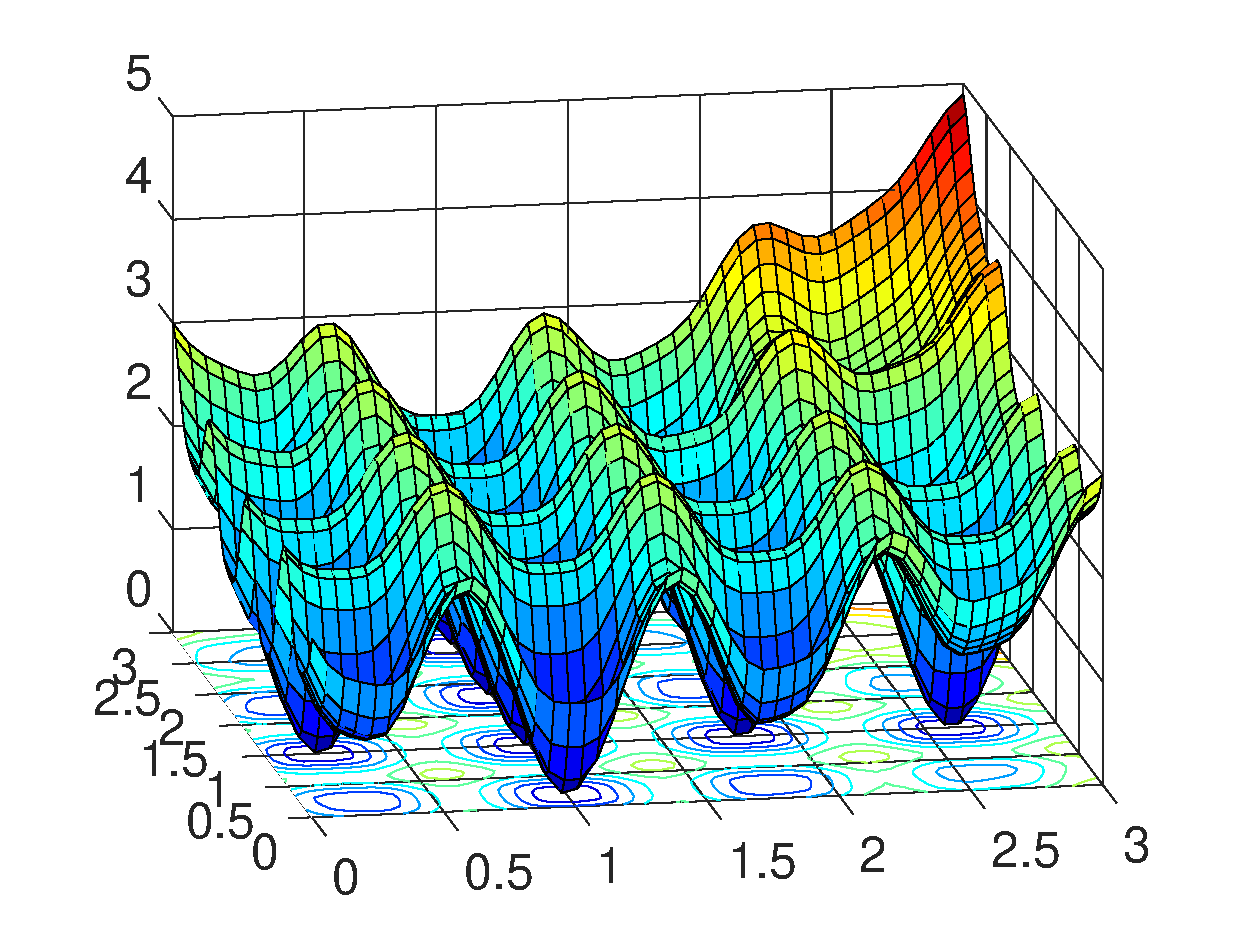
\includegraphics[width=0.98\textwidth]{chapters/minimization-fx/mfiles/fxxq3/surfcfx3.eps}
         \caption{Superfície $e(\VECTOR{x})$. }
         \label{fig:ex:minfxbCfxbaxqaxq3:a}
     \end{subfigure}
     \hfill
     \begin{subfigure}[b]{0.49\textwidth}
         \centering
         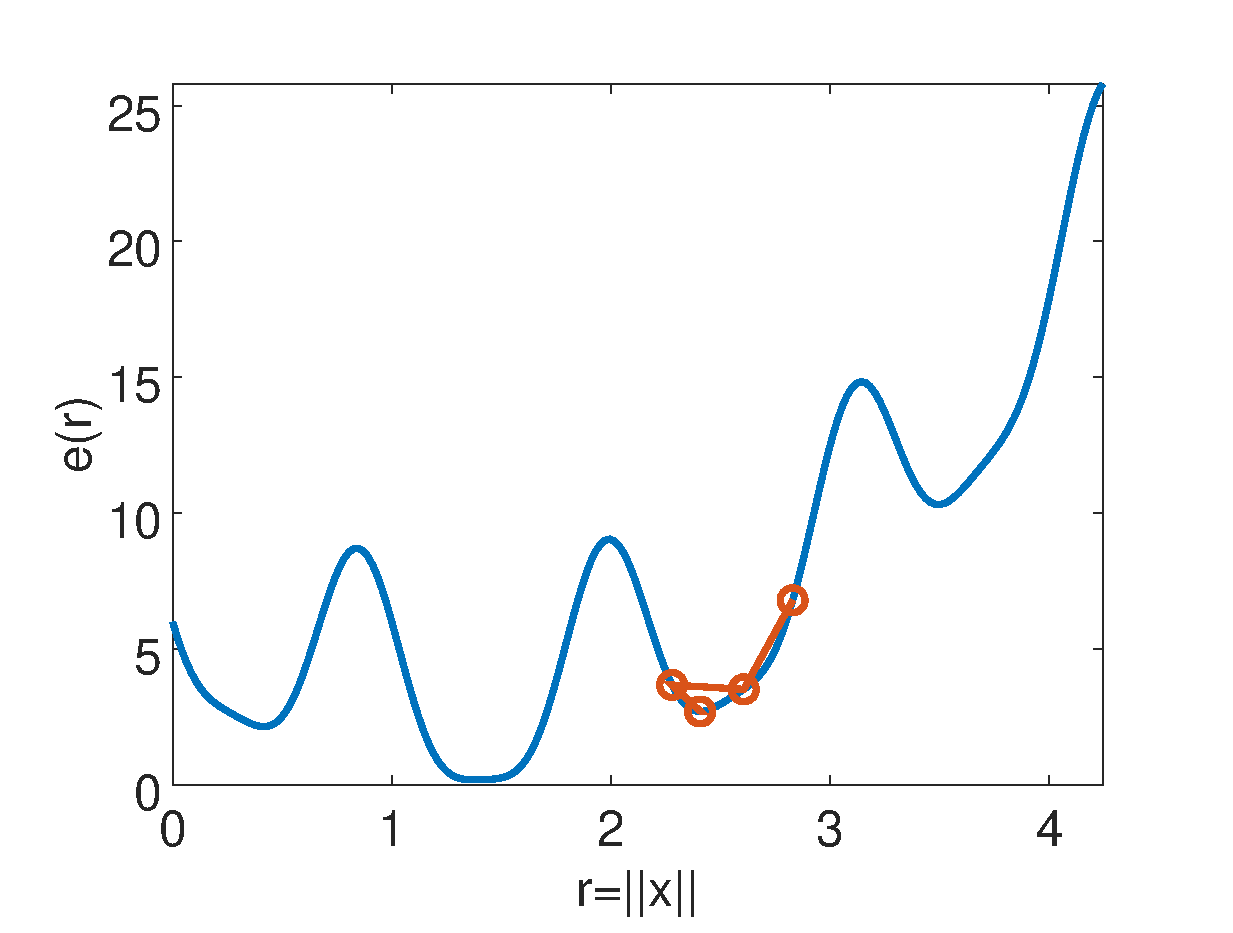
\includegraphics[width=0.98\textwidth]{chapters/minimization-fx/mfiles/fxxq3/plotfx3.eps}
         \caption{Curva $e(\VECTOR{x})$ na direção $(1,1)$.}
         \label{fig:ex:minfxbCfxbaxqaxq3:b}
     \end{subfigure}
        \caption{Resposta gráfica do Exemplo \ref{ex:minfxbCfxbaxqaxq1}. }
        \label{fig:ex:minfxbCfxbaxqaxq3}
\end{figure}

\begin{SolutionT}[Relativa ao Exemplo \ref{ex:minfxbCfxbaxqaxq1}:]
\label{ex:minfxbCfxbaxqaxq3:sol2}
Se escolhemos o ponto inicial $\VECTOR{x}_0=[\frac{11.0999}{5}$ $\frac{11.0999}{5}]^{\transpose}$,
com pendente\footnote{O cálculo da
pendente de $e(\VECTOR{\hat{x}})$ pode ser visto no Teorema \ref{theo:derfxbCfxb0}.} 
$\frac{\partial e(\VECTOR{x}_0)}{\partial \VECTOR{x} }=[0.44442\quad 0.44442]^{\transpose}$ e 
usamos iterativamente a Eq. (\ref{eq:minfxbCfxbaxqaxq2}), obtemos os valores 
$\VECTOR{x}_k$ e $e(\VECTOR{x}_k)$, como mostra a Tabela \ref{table:ex:minfxbCfxbaxqaxq4},
onde se assume o final do processo iterativo quando $\VECTOR{x}_k \approx \VECTOR{x}_{k-1}$.
Assim, a aproximação iterativa conclui na resposta 
$\VECTOR{\hat{x}}\approx \VECTOR{x}_{7} =[0.97172\quad 0.97172]^{\transpose}$
com um erro $e(\VECTOR{\hat{x}})=0.19325$ e uma pendente
$\frac{\partial e(\VECTOR{\hat{x}})}{\partial \VECTOR{x} }=[-0.0037461\quad -0.0037461]^{\transpose}$;
este processo pode ser visto de forma gráfica na Figura \ref{fig:ex:minfxbCfxbaxqaxq4:b}.
\end{SolutionT}


\begin{table}[h!]
\centering
\begin{tabular}{|l|l|l|l|l|l|l|l|l|}
\hline
$k$ & 0 & 1 & 2 & 3 & 4 & 5 & 6 & 7\\ \hline
$\VECTOR{x}_k$ & 2.21998 & 2.15837 & 1.27881 & 1.02790 & 0.98814 & 0.96083 & 0.97294 & 0.97172 \\ 
~              & 2.21998 & 2.15837 & 1.27881 & 1.02790 & 0.98814 & 0.96083 & 0.97294 & 0.97172 \\ \hline
$||\VECTOR{x}_k||$ & 3.1395 & 3.0524 & 1.8085 & 1.4537 & 1.3974 & 1.3588 & 1.3759 & 1.3742 \\ \hline
$e(\VECTOR{x}_k)$ & 14.84107 & 13.88071 & 5.63225 & 0.21557 & 0.19588 & 0.19518 & 0.19326 & 0.19325 \\ \hline
\end{tabular}
\caption{Resposta iterativa do Exemplo \ref{ex:minfxbCfxbaxqaxq1}.}
\label{table:ex:minfxbCfxbaxqaxq4}
\end{table}

     \begin{figure}[!h]
         \centering
         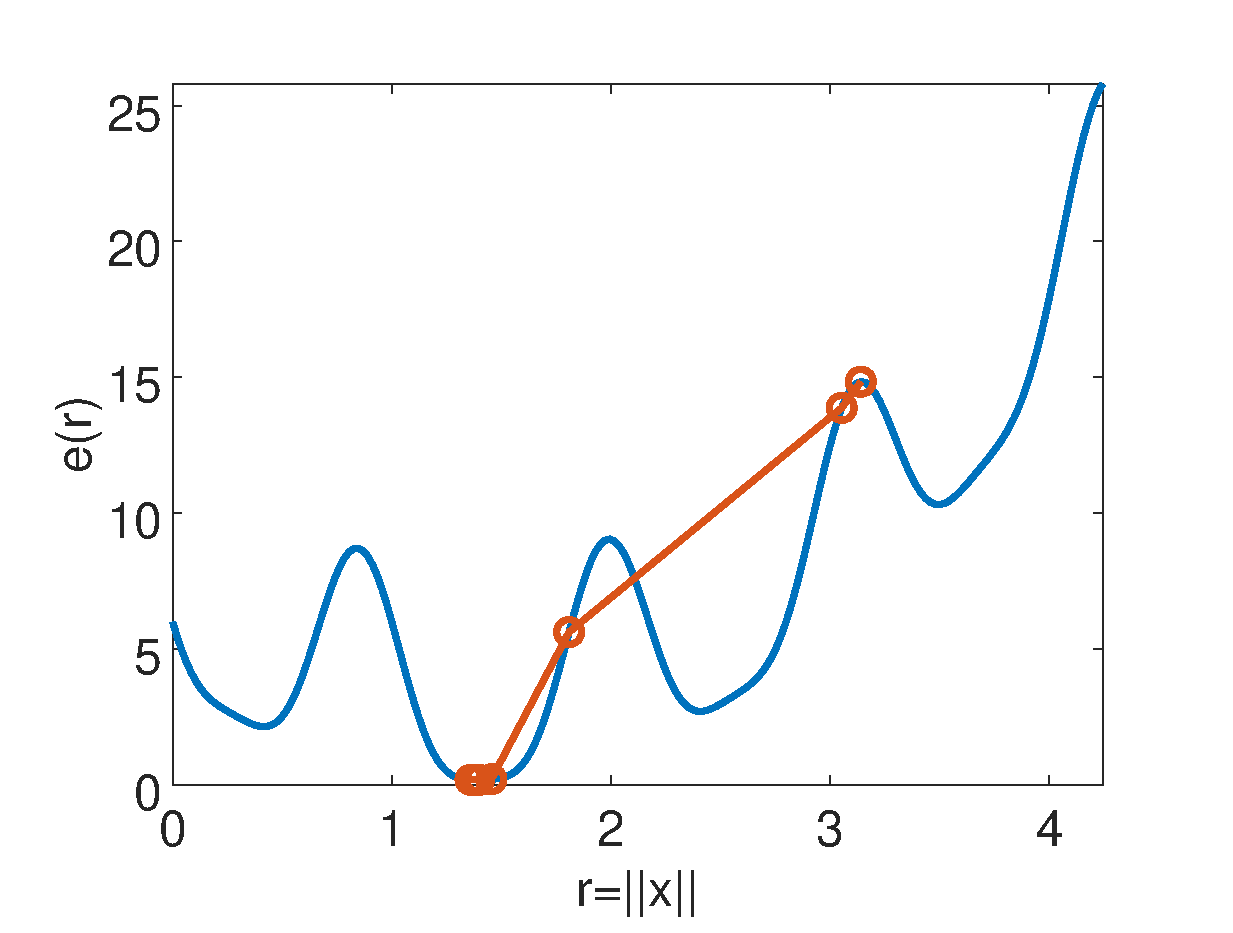
\includegraphics[width=0.5\textwidth]{chapters/minimization-fx/mfiles/fxxq3/plotfx4.eps}
         \caption{Curva $e(\VECTOR{x})$ na direção $(1,1)$.}
         \label{fig:ex:minfxbCfxbaxqaxq4:b}
     \end{figure}



\newpage

\section{Minimização de $||\VECTOR{f}(\VECTOR{x})-\VECTOR{b}||_{\MATRIX{C}}^2+\alpha||\VECTOR{x}-\VECTOR{x}_{last}||_{\MATRIX{D}}^2$}


\index{Minimização, métodos!Regularização de Tikhonov}
\index{Problema inverso!Não linear}
\index{Minimização do erro quadrático!Não linear}

\begin{theorem}[Solução iterativa]\label{theo:minfxbCfxbaxoaxo}
Dados,
os vetores coluna $\VECTOR{x}\in \mathbb{R}^N$, $\VECTOR{b}\in \mathbb{R}^M$ e $\VECTOR{x}_{last}\in \mathbb{R}^N$,  
uma função $\VECTOR{f}:\mathbb{R}^{N} \rightarrow \mathbb{R}^{M}$, 
as matrizes diagonais $\MATRIX{C} \in \mathbb{R}^{M\times M}$ e $\MATRIX{D} \in \mathbb{R}^{N\times N}$, e 
definida a Eq. (\ref{eq:minfxbCfxbaxoaxo1}),
\begin{equation}\label{eq:minfxbCfxbaxoaxo1}
e(\VECTOR{x})=||\VECTOR{f}(\VECTOR{x})-\VECTOR{b}||_{\MATRIX{C}}^2+\alpha||\VECTOR{x}-\VECTOR{x}_{last}||_{\MATRIX{D}}^2,
\end{equation}
tendo en consideração que $\VECTOR{x}_{last}$ é uma constante equivalente a $\VECTOR{x}_{k-1}$
numa busca iterativa; é dizer, o segundo somando na Eq. (\ref{eq:minfxbCfxbaxoaxo1}) 
procura minimizar $||\VECTOR{x}_{k}-\VECTOR{x}_{k-1}||_{\MATRIX{D}}^2$.


Se desejamos ter o ponto $\VECTOR{\hat{x}}$ que minimiza o escalar $e(\VECTOR{\hat{x}})$,
podemos achar este ponto usando iterativamente a Eq. (\ref{eq:minfxbCfxbaxoaxo2}),
onde  $\MATRIX{J}(\VECTOR{x})$ é a \hyperref[def:jacobian]{\textbf{matriz Jacobiana}}  de $\VECTOR{f}(\VECTOR{x})$.
\begin{equation}\label{eq:minfxbCfxbaxoaxo2}
\VECTOR{x}_{k}\leftarrow \VECTOR{x}_{k-1}+
\left[ \MATRIX{J}(\VECTOR{x}_{k-1})^{\transpose}\MATRIX{C} \MATRIX{J}(\VECTOR{x}_{k-1}) +\alpha\MATRIX{D} \right]^{-1}
 \left[\MATRIX{J}(\VECTOR{x}_{k-1})^{\transpose}\MATRIX{C}\left\{\VECTOR{b}-\VECTOR{f}(\VECTOR{x}_{k-1})\right\}\right] 
\end{equation}
Assim, $\VECTOR{\hat{x}}$ pode ser achado 
iniciando a Eq. (\ref{eq:minfxbCfxbaxoaxo2}) desde um $\VECTOR{x}_{0}$ qualquer, 
ate que $\VECTOR{x}_{k}$ seja muito próximo a $\VECTOR{x}_{k-1}$,
onde se declara que $\VECTOR{\hat{x}} \approx \VECTOR{x}_{k}$,
que corresponde a um mínimo\footnote{\label{ref:minfx}A
demostração pode ser vista na Prova \ref{proof:theo:minfxbCfxbaxod}.} de $e(\VECTOR{x})$,
sem aclarar se é local ou global.


\textbf{Considerções:}

\begin{itemize}
\item É interessante verificar sempre na Eq. (\ref{eq:minfxbCfxbaxoaxo2}) 
se  $\MATRIX{J}(\VECTOR{x}_{k-1}) = \MATRIX{0}$,
pois indica que existe\footref{ref:minfx} um ponto de inflexão 
(máximo, mínimo ou ponto de sela) em $e(\VECTOR{x}_{k-1})$;
consequentemente poderiamos ter achado um mínimo.
\item A busca iterativa da Eq. (\ref{eq:minfxbCfxbaxoaxo2}) é considerada falida quando 
$\MATRIX{J}(\VECTOR{x}_{k-1})^{\transpose}\MATRIX{C} \MATRIX{J}(\VECTOR{x}_{k-1}) -\alpha\MATRIX{D}$
não tem inversa.
\end{itemize}


\end{theorem} 


\newpage

\section{Provas dos teoremas}
 
%%%%%%%%%%%%%%%%%%%%%%%%%%%%%%%%%%%%%%%%%%%%%%%%%%%%%%%%%%%%%%%%%%%%%%%%%%%%%%%%%%%%%%%
%%%%%%%%%%%%%%%%%%%%%%%%%%%%%%%%%%%%%%%%%%%%%%%%%%%%%%%%%%%%%%%%%%%%%%%%%%%%%%%%%%%%%%%
\begin{myproofT}[Prova do Teorema \ref{theo:minAxbCAxb}:]\label{proof:theo:minAxbCAxb}
Dados,
os vetores coluna $\VECTOR{x}\in \mathbb{R}^N$ e $\VECTOR{b}\in \mathbb{R}^M$,  
uma matriz $\MATRIX{A} \in \mathbb{R}^{M\times N}$, 
uma matriz diagonal $\MATRIX{C} \in \mathbb{R}^{M\times M}$, e 
definida a Eq. (\ref{eq:proof:minAxbCAxb0}),
\begin{equation}\label{eq:proof:minAxbCAxb0}
e(\VECTOR{x})=||\MATRIX{A}\VECTOR{x}-\VECTOR{b}||_{\MATRIX{C}}^2.
\end{equation}
Para achar o ponto $\VECTOR{\hat{x}}$ que gere o menor valor de $e(\VECTOR{\hat{x}})$, é aplicado
o critério que um ponto de inflexão pode ser achado quando 
$\frac{\partial e(\VECTOR{\hat{x}})}{\partial \VECTOR{x} }=[0~ 0~ \hdots~ 0 ]^{\transpose}$.
Assim, usando o Corolário \ref{coro:derAxbAxb2} podemos 
rescrever esta igualdade como a Eq. (\ref{eq:proof:minAxbCAxb1}),
\begin{equation}\label{eq:proof:minAxbCAxb1}
2 \MATRIX{A}^{\transpose}\MATRIX{C}\left(\MATRIX{A}\VECTOR{\hat{x}}-\VECTOR{b}\right)=[0~ 0~ \hdots~ 0 ]^{\transpose},
\end{equation}
de modo que pode ser obtido:
\begin{equation}\label{eq:proof:minAxbCAxb2}
\VECTOR{\hat{x}}=\left( \MATRIX{A}^{\transpose}\MATRIX{C}\MATRIX{A} \right)^{-1} \MATRIX{A}^{\transpose}\MATRIX{C} \VECTOR{b}.
\end{equation}
Dado que  a função $e(\VECTOR{x})$ é sempre positiva, o que implica a existencia de um mínimo,
e que o ponto de inflexão $\VECTOR{\hat{x}}$ encontrado na Eq. (\ref{eq:proof:minAxbCAxb2}) é único, 
podemos concluir que  $\VECTOR{\hat{x}}$ é o mínimo global da Eq. (\ref{eq:proof:minAxbCAxb0}).
\end{myproofT}

%%%%%%%%%%%%%%%%%%%%%%%%%%%%%%%%%%%%%%%%%%%%%%%%%%%%%%%%%%%%%%%%%%%%%%%%%%%%%%%%%%%%%%%
%%%%%%%%%%%%%%%%%%%%%%%%%%%%%%%%%%%%%%%%%%%%%%%%%%%%%%%%%%%%%%%%%%%%%%%%%%%%%%%%%%%%%%%
\begin{myproofT}[Prova do Teorema \ref{theo:minAxbCAxbplusalphaxqD}:]
\label{proof:theo:minAxbCAxbalphaxqD}
Dados,
os vetores coluna $\VECTOR{x}\in \mathbb{R}^N$, $\VECTOR{b}\in \mathbb{R}^M$ e $\VECTOR{q}\in \mathbb{R}^N$,  
uma matriz $\MATRIX{A} \in \mathbb{R}^{M\times N}$, 
as matrizes diagonais $\MATRIX{C} \in \mathbb{R}^{M\times M}$ e $\MATRIX{D} \in \mathbb{R}^{N\times N}$, e 
definida a Eq. (\ref{eq:proof:minAxbCAxb0alphaxqD}),
\begin{equation}\label{eq:proof:minAxbCAxb0alphaxqD}
e(\VECTOR{x})=||\MATRIX{A}\VECTOR{x}-\VECTOR{b}||_{\MATRIX{C}}^2+\alpha||\VECTOR{x}-\VECTOR{q}||_{\MATRIX{D}}^2.
\end{equation}
Para achar o ponto $\VECTOR{\hat{x}}$ que gere o menor valor de $e(\VECTOR{\hat{x}})$, é aplicado
o critério que um ponto de inflexão pode ser achado quando 
$\frac{\partial e(\VECTOR{\hat{x}})}{\partial \VECTOR{x} }=[0~ 0~ \hdots~ 0 ]^{\transpose}$.
Assim, usando o Corolário \ref{coro:derAxbAxb2} podemos 
rescrever esta igualdade como a Eq. (\ref{eq:proof:minAxbCAxb1alphaxqD}),
\begin{equation}\label{eq:proof:minAxbCAxb1alphaxqD}
2 \MATRIX{A}^{\transpose}\MATRIX{C}\left(\MATRIX{A}\VECTOR{\hat{x}}-\VECTOR{b}\right)
+2 \alpha\MATRIX{D}\left(\VECTOR{\hat{x}}-\VECTOR{q}\right)=[0~ 0~ \hdots~ 0 ]^{\transpose},
\end{equation}
de modo que pode ser obtido:
\begin{equation}\label{eq:proof:minAxbCAxb2alphaxqD}
\VECTOR{\hat{x}}=\left[ \MATRIX{A}^{\transpose}\MATRIX{C}\MATRIX{A} +\alpha\MATRIX{D}\right]^{-1} 
\left[ \MATRIX{A}^{\transpose}\MATRIX{C} \VECTOR{b}+\alpha\MATRIX{D}\VECTOR{q}\right].
\end{equation}
Dado que  a função $e(\VECTOR{x})$ é sempre positiva, o que implica a existencia de um mínimo,
e que o ponto de inflexão $\VECTOR{\hat{x}}$ encontrado na Eq. (\ref{eq:proof:minAxbCAxb2alphaxqD}) é único, 
podemos concluir que  $\VECTOR{\hat{x}}$ é o mínimo global da Eq. (\ref{eq:proof:minAxbCAxb0alphaxqD}).
\end{myproofT}

%%%%%%%%%%%%%%%%%%%%%%%%%%%%%%%%%%%%%%%%%%%%%%%%%%%%%%%%%%%%%%%%%%%%%%%%%%%%%%%%%%%%%%%
%%%%%%%%%%%%%%%%%%%%%%%%%%%%%%%%%%%%%%%%%%%%%%%%%%%%%%%%%%%%%%%%%%%%%%%%%%%%%%%%%%%%%%%
\begin{myproofT}[Prova do Teorema \ref{theo:minfxbCfxb}]\label{proof:theo:minfxbCfxb}
Dados,
os vetores coluna $\VECTOR{x}\in \mathbb{R}^N$ e $\VECTOR{b}\in \mathbb{R}^M$,  
uma função $\VECTOR{f}:\mathbb{R}^{N} \rightarrow \mathbb{R}^{M}$, 
uma matriz diagonal $\MATRIX{C} \in \mathbb{R}^{M\times M}$, e 
definida a Eq. (\ref{eq:proof:minfxbCfxb0}),
\begin{equation}\label{eq:proof:minfxbCfxb0}
e(\VECTOR{x})=||\VECTOR{f}(\VECTOR{x})-\VECTOR{b}||_{\MATRIX{C}}^2;
\end{equation}
sabemos que para achar o ponto $\VECTOR{\hat{x}}$ que gere o menor valor de $e(\VECTOR{\hat{x}})$, é aplicado
o critério que um ponto de inflexão $\VECTOR{x}^+$; é dizer, um máximo, um mínimo ou um ponto de sela, pode ser achado quando 
$\frac{\partial e(\VECTOR{x}^+)}{\partial \VECTOR{x} }=[0~ 0~ \hdots~ 0 ]^{\transpose}$, como pode ser visto na Figura \ref{fig:ex0b};
assim, usando o Teorema \ref{theo:derfxbCfxb0} obtemos que
\begin{equation}\label{eq:proof:minfxbCfxb1exact}
2 \MATRIX{J}(\VECTOR{x}^+)^{\transpose}\MATRIX{C}\left[ \VECTOR{f}(\VECTOR{x}^+)-\VECTOR{b} \right] =
\frac{\partial e(\VECTOR{x}^+)}{\partial \VECTOR{x} }=[0~ 0~ \hdots~ 0 ]^{\transpose},
\end{equation}
Da Eq. (\ref{eq:proof:minfxbCfxb1exact}) observamos, que podemos achar pontos de inflexão $\VECTOR{x}^+$
em $e(\VECTOR{x}^+)$ quando 
$\MATRIX{J}(\VECTOR{x}^+) \equiv \frac{\partial \VECTOR{f}(\VECTOR{x}^+)}{\partial \VECTOR{x}^{\transpose} } = \MATRIX{0}$, 
sem importar o nível de proximidade entre os vetores $\VECTOR{b}$ e $\VECTOR{f}(\VECTOR{x}^+)$;
é dizer não precisa ser um mínimo global, só um ponto de inflexão qualquer
(máximo, mínimo ou ponto de sela).

\begin{figure}[!h]
     \centering
     \begin{subfigure}[b]{0.48\textwidth}
         \centering
         \includegraphics[width=0.8\textwidth]{chapters/minimization-fx/minimoex2.eps}
         \caption{$\VECTOR{b} \neq \VECTOR{f}(\VECTOR{x})$.}
         \label{fig:ex0b}
     \end{subfigure}
     \hfill
     \begin{subfigure}[b]{0.48\textwidth}
         \centering
         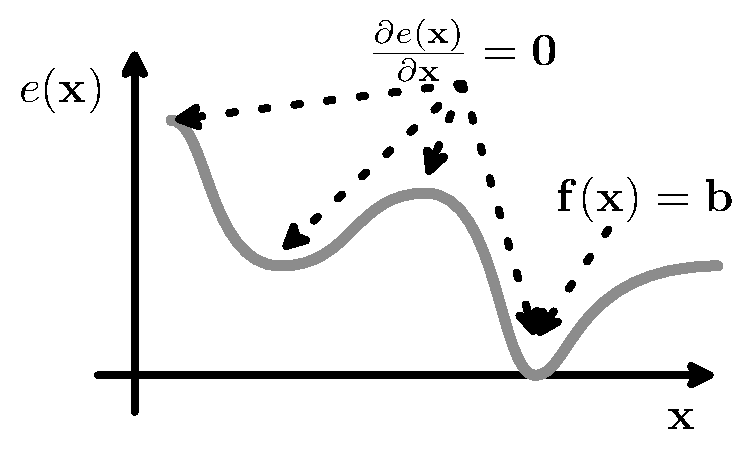
\includegraphics[width=0.8\textwidth]{chapters/minimization-fx/minimoex1.eps}
         \caption{$\VECTOR{b} \approx \VECTOR{f}(\VECTOR{x})$.}
         \label{fig:ex0a}
     \end{subfigure}
        \caption{Possibilidades para $\frac{\partial e(\VECTOR{x})}{\partial \VECTOR{x} }$.}
        \label{fig:ex0}
\end{figure}


Por outro lado, podemos realizar uma aproximação linear de $\VECTOR{f}(\VECTOR{x})$ em $e(\VECTOR{x})$
ao redor do ponto $\VECTOR{p}$ usando a \hyperref[def:taylor]{\textbf{serie de Taylor}},
de modo que a Eq. (\ref{eq:proof:minfxbCfxb0}) pode ficar expresada como
\begin{equation}\label{eq:proof:minfxbCfxb0approx}
e(\VECTOR{x}) \approx ||\MATRIX{J}(\VECTOR{p})(\VECTOR{x}-\VECTOR{p})-(\VECTOR{b}-\VECTOR{f}(\VECTOR{p}))||_{\MATRIX{C}}^2,
\end{equation}
onde $\MATRIX{J}(\VECTOR{p})$ representa a \hyperref[def:jacobian]{\textbf{matriz Jacobiana}} 
de $\VECTOR{f}(\VECTOR{x})$ avaliada no ponto $\VECTOR{p}$.
Assim, usando o resultado da Prova \ref{proof:theo:minAxbCAxb} na Eq. (\ref{eq:proof:minfxbCfxb0approx}), 
podemos concluir que um ponto $\VECTOR{x}^*$ que é 
um mínimo da aproximação linear feita em $e(\VECTOR{x})$ ao redor do ponto $\VECTOR{p}$,
pode ser achado como
\begin{equation}\label{eq:proof:minAxbCAxb2approx}
\VECTOR{x}^* \approx \VECTOR{p}+ \left[ \MATRIX{J}(\VECTOR{p})^{\transpose}\MATRIX{C}\MATRIX{J}(\VECTOR{p}) \right]^{-1} \MATRIX{J}(\VECTOR{p})^{\transpose}\MATRIX{C} \left[\VECTOR{b}-\VECTOR{f}(\VECTOR{p})\right].
\end{equation}


Desta equação podemos tirar a seguintes conclusões:
\begin{itemize}

\item Observamos que a posição $\VECTOR{p}$ é corregida para ficar próximo à posição $\VECTOR{x}^*$, 
que é o valor mínimo na aproximação linear ao redor de $\VECTOR{p}$;
pelo que se deduz que a Eq. (\ref{eq:proof:minAxbCAxb2approx})
pode ser usada para procurar aproximações de pontos mínimos $\VECTOR{\hat{x}}$ em $e(\VECTOR{x})$ desde a posição $\VECTOR{p}$,
ou pelo menos aproximações de novas posições em caminhos numa direção descendente de $e(\VECTOR{x})$.

\item A Eq. (\ref{eq:proof:minAxbCAxb2approx}) é satisfeita 
com $\VECTOR{x}^* \approx \VECTOR{p}$ se acharmos um  
ponto $\VECTOR{p}$ onde  $\VECTOR{b} \approx \VECTOR{f}(\VECTOR{p})$; 
é dizer um mínimo global de $e(\VECTOR{x})$ em $\VECTOR{p}$, como pode ser visto na Figura \ref{fig:ex0a}. 

\item Se reescrevemos a Eq. (\ref{eq:proof:minAxbCAxb2approx}) usando o Teorema \ref{theo:derfxbCfxb0},
obtemos
\begin{equation}\label{eq:proof:minfxbCfxb2ea}
\VECTOR{x}^* \approx \VECTOR{p} -
0.5 \left[ \MATRIX{J}(\VECTOR{p})^{\transpose}\MATRIX{C} \MATRIX{J}(\VECTOR{p}) \right]^{-1}
\frac{\partial e(\VECTOR{p})}{\partial \VECTOR{x} },
\end{equation}
onde a Eq. (\ref{eq:proof:minfxbCfxb2ea}) é satisfeita 
com $\VECTOR{x}^* \approx \VECTOR{p}$
se acharmos um  ponto $\VECTOR{p}$ onde  
$\frac{\partial e(\VECTOR{p})}{\partial \VECTOR{x} }\approx \VECTOR{0}$; 
é dizer $\VECTOR{p}$ é um ponto de inflexão de $e(\VECTOR{x})$, como pode ser visto na Figura \ref{fig:ex0b}.
Porem, dado que a equação avança desde $\VECTOR{p}$ na direção de um mínimo $\VECTOR{x}^*$, 
mesmo que nos pontos de inflexão correspondentes a máximos ou pontos de sela,
encontremos valores de $\VECTOR{p}$ próximos a $\VECTOR{x}^*$,
 estes casos serão pouco estáveis pois
a correção da posição $\VECTOR{p}$ será na direção de um mínimo e não do máximo.

\item Se modificamos a Eq. (\ref{eq:proof:minAxbCAxb2approx}), e escolhemos um ponto  
$\VECTOR{p}_0$ que consideremos próximo ao ponto $\VECTOR{\hat{x}}$ que minimiza $e(\VECTOR{\hat{x}})$,
podemos achar iterativamente aproximações lineares $\VECTOR{x}^*$ cada vez mais próximos a  $\VECTOR{\hat{x}}$,
se usamos a seguinte equação iterativa,
\begin{equation}\label{eq:proof:minfxbCfxb3}
\VECTOR{p}_{k} \leftarrow \VECTOR{p}_{k-1} -
\left[ \MATRIX{J}(\VECTOR{p}_{k-1})^{\transpose}\MATRIX{C} \MATRIX{J}(\VECTOR{p}_{k-1}) \right]^{-1}
\MATRIX{J}(\VECTOR{p}_{k-1})^{\transpose}\MATRIX{C} \left(\VECTOR{f}(\VECTOR{p}_{k-1})-\VECTOR{b}\right),
\end{equation}
iniciando desde um $\VECTOR{p}_{0}$ 
ate que exista uma tendencia prolongada onde se observe que $\VECTOR{p}_{k}$ é muito próximo a $\VECTOR{p}_{k-1}$,
momento no qual declaramos que $\VECTOR{\hat{x}} \approx \VECTOR{p}_{k}$.
\item Como foi visto na Figura  \ref{fig:ex0b},
pode existir um mínimo global $\VECTOR{\hat{x}}$ de $e(\VECTOR{\hat{x}})>0$.
Isto nos restringe a que no uso da Eq. (\ref{eq:proof:minfxbCfxb3}),
nosso critério principal para estabelecer o final do cáculo iterativo,
deve ser a tendencia na  proximidade entre $\VECTOR{p}_{k}$ e $\VECTOR{p}_{k-1}$ 
e não o valor de $e(\VECTOR{x}_k)$.
\end{itemize}~

Um diagrama completo resumindo todas estas conclusões pode ser visto na Figura \ref{fig:fluxo1}.
\end{myproofT}
\begin{figure}[!h]
     \centering
         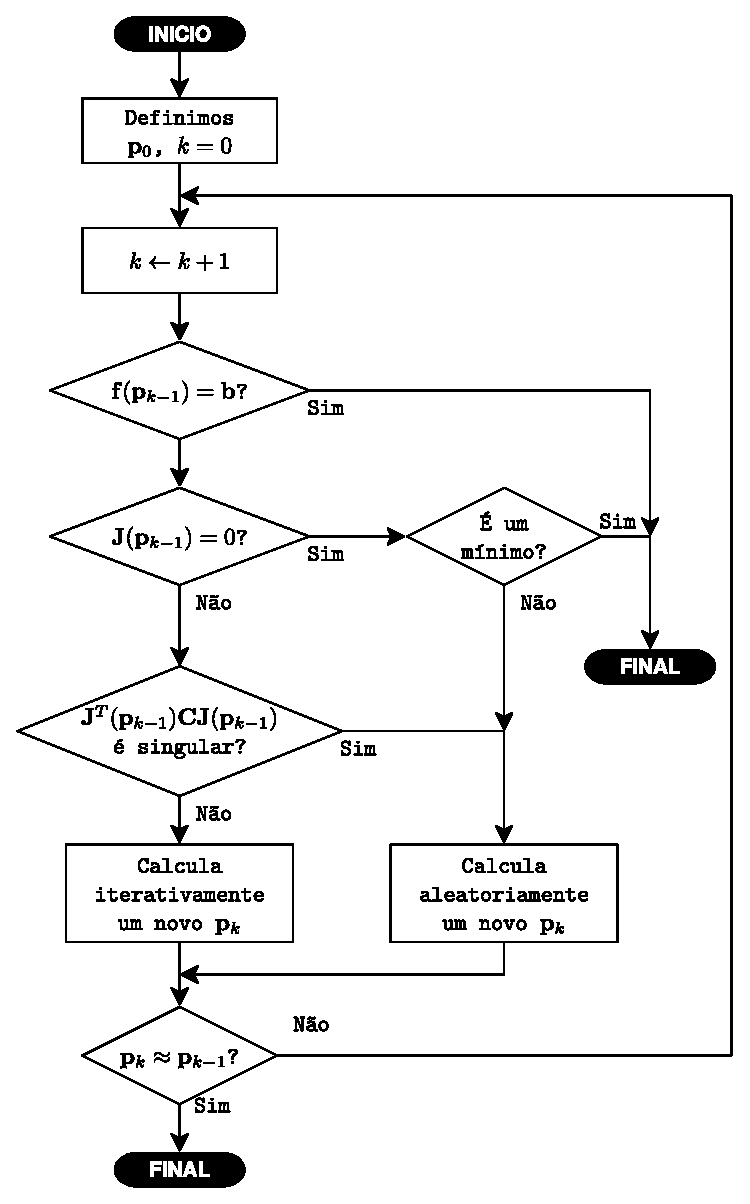
\includegraphics[width=0.75\textwidth]{chapters/minimization-fx/fluxo1.eps}
        \caption{Diagrama de fluxo da solução iterativa para achar um mínimo, seguindo a Prova \ref{proof:theo:minfxbCfxb}.}
        \label{fig:fluxo1}
\end{figure}


%%%%%%%%%%%%%%%%%%%%%%%%%%%%%%%%%%%%%%%%%%%%%%%%%%%%%%%%%%%%%%%%%%%%%%%%%%%%%%%%%%%%%%%
%%%%%%%%%%%%%%%%%%%%%%%%%%%%%%%%%%%%%%%%%%%%%%%%%%%%%%%%%%%%%%%%%%%%%%%%%%%%%%%%%%%%%%%
\begin{myproofT}[Prova do Teorema \ref{theo:minfxbCfxbaxqaxq}]\label{proof:theo:minfxbCfxbaxqd}
Dados,
um escalar $\alpha\in \mathbb{R}$,
os vetores coluna $\VECTOR{x}\in \mathbb{R}^N$, 
$\VECTOR{q}\in \mathbb{R}^N$ e
$\VECTOR{b}\in \mathbb{R}^M$,  
uma função $\VECTOR{f}:\mathbb{R}^{N} \rightarrow \mathbb{R}^{M}$, 
as matrizes diagonais $\MATRIX{C} \in \mathbb{R}^{M\times M}$ e $\MATRIX{D} \in \mathbb{R}^{N\times N}$, e 
definida a Eq. (\ref{eq:proof:minfxbCfxbaxqd0}),
\begin{equation}\label{eq:proof:minfxbCfxbaxqd0}
e(\VECTOR{x})=||\VECTOR{f}(\VECTOR{x})-\VECTOR{b}||_{\MATRIX{C}}^2+\alpha||\VECTOR{x}-\VECTOR{q}||_{\MATRIX{D}}^2;
\end{equation}
sabemos que para achar o ponto $\VECTOR{\hat{x}}$ que gere o menor valor de $e(\VECTOR{\hat{x}})$, é aplicado
o critério que um ponto de inflexão $\VECTOR{x}^+$; é dizer, um máximo, um mínimo ou um ponto de sela, pode ser achado quando 
$\frac{\partial e(\VECTOR{x}^+)}{\partial \VECTOR{x} }=[0~ 0~ \hdots~ 0 ]^{\transpose}$ (ver Figura \ref{fig:ex0b});
assim, usando o Teorema \ref{theo:derfxbCfxb0} e o Corolário \ref{coro:derAxbAxb2} obtemos que
\begin{equation}\label{eq:proof:minfxbCfxb1exact2}
2 \MATRIX{J}(\VECTOR{x}^+)^{\transpose}\MATRIX{C}\left[ \VECTOR{f}(\VECTOR{x}^+)-\VECTOR{b} \right] +
2 \alpha\MATRIX{D}\left[\VECTOR{x}^+-\VECTOR{q}\right]
=
\frac{\partial e(\VECTOR{x}^+)}{\partial \VECTOR{x} }=[0~ 0~ \hdots~ 0 ]^{\transpose},
\end{equation}
Da Eq. (\ref{eq:proof:minfxbCfxb1exact2}) observamos, 
que podemos achar um ponto de inflexão $\VECTOR{q}$
em $e(\VECTOR{q})$ se 
$\MATRIX{J}(\VECTOR{q})  = \MATRIX{0}$ ou um mínimo geral se $\VECTOR{f}(\VECTOR{q})=\VECTOR{b}$,
caso contrario, 
se nenhuma destas possibilidades são cumpridas devemos aplicar outros critérios para achar os pontos de inflexão.

Assim, procurando outros critérios, podemos realizar uma aproximação linear de $\VECTOR{f}(\VECTOR{x})$ em $e(\VECTOR{x})$
ao redor do ponto $\VECTOR{p}$ usando a \hyperref[def:taylor]{\textbf{serie de Taylor}},
de modo que a Eq. (\ref{eq:proof:minfxbCfxbaxqd0}) pode ficar expressada como
\begin{equation}\label{eq:proof:minfxbCfxb0alphaxqDapprox}
e(\VECTOR{x}) \approx 
||\MATRIX{J}(\VECTOR{p})[\VECTOR{x}-\VECTOR{p}]-[\VECTOR{b}-\VECTOR{f}(\VECTOR{p})]||_{\MATRIX{C}}^2+
\alpha||[\VECTOR{x}-\VECTOR{p}]-[\VECTOR{q}-\VECTOR{p}]||_{\MATRIX{D}}^2,
\end{equation}
onde $\MATRIX{J}(\VECTOR{p})$ representa a \hyperref[def:jacobian]{\textbf{matriz Jacobiana}} 
de $\VECTOR{f}(\VECTOR{x})$ avaliada no ponto $\VECTOR{p}$.
Assim, usando o resultado da Prova \ref{proof:theo:minAxbCAxbalphaxqD} na Eq. (\ref{eq:proof:minfxbCfxb0alphaxqDapprox}), 
podemos concluir que um ponto $\VECTOR{x}^*$ que é 
um mínimo da aproximação linear feita em $e(\VECTOR{x})$ ao redor do ponto $\VECTOR{p}$,
pode ser achado como
\begin{equation}\label{eq:proof:minfxbCfxbaxqd2}
\VECTOR{x}^* \approx \VECTOR{p} +
\left[ \MATRIX{J}(\VECTOR{p})^{\transpose}\MATRIX{C} \MATRIX{J}(\VECTOR{p})+\alpha \MATRIX{D} \right]^{-1}
\left\{ \MATRIX{J}(\VECTOR{p})^{\transpose}\MATRIX{C} \left[\VECTOR{b}-\VECTOR{f}(\VECTOR{p})\right]-\alpha\MATRIX{D}[\VECTOR{p}-\VECTOR{q}]\right\}.
\end{equation}


Desta equação podemos tirar a seguintes conclusões:
\begin{itemize}

\item Observamos que a posição $\VECTOR{p}$ é corregida para ficar próximo à posição $\VECTOR{x}^*$, 
que é o valor mínimo na aproximação linear ao redor de $\VECTOR{p}$;
pelo que se deduz que a Eq. (\ref{eq:proof:minfxbCfxbaxqd2})
pode ser usada para procurar aproximações de pontos mínimos $\VECTOR{\hat{x}}$ em $e(\VECTOR{x})$ desde a posição $\VECTOR{p}$,
ou pelo menos aproximações de novas posições em caminhos numa direção descendente de $e(\VECTOR{x})$.

\begin{comment}
\item A Eq. (\ref{eq:proof:minfxbCfxbaxqd2}) é satisfeita 
com $\VECTOR{x}^* \approx \VECTOR{p}$ se acharmos um  
ponto $\VECTOR{p}$ onde  $\VECTOR{b} \approx \VECTOR{f}(\VECTOR{p}\approx \VECTOR{q})$; 
é dizer um mínimo global de $e(\VECTOR{x})$ em $\VECTOR{p}$, como pode ser visto na Figura \ref{fig:ex0a}. 
\end{comment}

\item Se reescrevemos a Eq. (\ref{eq:proof:minfxbCfxbaxqd2}) usando o Teorema \ref{theo:derfxbCfxb0}
e o Corolário \ref{coro:derAxbAxb2},
obtemos
\begin{equation}\label{eq:proof:minfxbCfxb2ea1}
\VECTOR{x}^* \approx \VECTOR{p} -
0.5 \left[ \MATRIX{J}(\VECTOR{p})^{\transpose}\MATRIX{C} \MATRIX{J}(\VECTOR{p})+\alpha \MATRIX{D} \right]^{-1}
\frac{\partial e(\VECTOR{p})}{\partial \VECTOR{x} },
\end{equation}
onde a Eq. (\ref{eq:proof:minfxbCfxb2ea1}) é satisfeita 
com $\VECTOR{x}^* \approx \VECTOR{p}$
se acharmos um  ponto $\VECTOR{p}$ onde  
$\frac{\partial e(\VECTOR{p})}{\partial \VECTOR{x} }\approx \VECTOR{0}$,
 como descrito na Eq. (\ref{eq:proof:minfxbCfxb1exact2}); 
é dizer $\VECTOR{p}$ é um ponto de inflexão de $e(\VECTOR{x})$, ver Figura \ref{fig:ex0b}.
Porem, dado que a equação avança desde $\VECTOR{p}$ na direção de um mínimo $\VECTOR{x}^*$, 
mesmo que nos pontos de inflexão correspondentes a máximos ou pontos de sela,
encontremos valores de $\VECTOR{p}$ próximos a $\VECTOR{x}^*$,
 estes casos serão pouco estáveis pois
a correção da posição $\VECTOR{p}$ será na direção de um mínimo e não do máximo.

\item Se modificamos a Eq. (\ref{eq:proof:minfxbCfxbaxqd2}), e escolhemos um ponto  
$\VECTOR{p}_0$ que consideremos próximo ao ponto $\VECTOR{\hat{x}}$ que minimiza $e(\VECTOR{\hat{x}})$,
podemos achar iterativamente aproximações lineares $\VECTOR{x}^*$ cada vez mais próximos a  $\VECTOR{\hat{x}}$,
se usamos a seguinte equação iterativa,
\begin{equation}\label{eq:proof:minfxbCfxb3a}
\VECTOR{p}_{k} \leftarrow \VECTOR{p}_{k-1} -
\left[ \MATRIX{J}(\VECTOR{p}_{k-1})^{\transpose}\MATRIX{C} \MATRIX{J}(\VECTOR{p}_{k-1}) +\alpha \MATRIX{D}\right]^{-1}
\left\{ \MATRIX{J}(\VECTOR{p}_{k-1})^{\transpose}\MATRIX{C} \left[\VECTOR{f}(\VECTOR{p}_{k-1})-\VECTOR{b}\right]+
\alpha\MATRIX{D}[\VECTOR{p}_{k-1}-\VECTOR{q}]\right\},
\end{equation}
iniciando desde um $\VECTOR{p}_{0}$ 
ate que exista uma tendencia prolongada onde se observe que $\VECTOR{p}_{k}$ é muito próximo a $\VECTOR{p}_{k-1}$,
momento no qual declaramos que $\VECTOR{\hat{x}} \approx \VECTOR{p}_{k}$.
\item Como foi visto na Figura  \ref{fig:ex0b},
pode existir um mínimo global $\VECTOR{\hat{x}}$ de $e(\VECTOR{\hat{x}}) > 0$.
Isto nos restringe a que no uso da Eq. (\ref{eq:proof:minfxbCfxb3a}),
nosso critério principal para estabelecer o final do cáculo iterativo,
deve ser a tendencia na  proximidade entre $\VECTOR{p}_{k}$ e $\VECTOR{p}_{k-1}$ 
e não o valor de $e(\VECTOR{x}_k)$.
\end{itemize}

Um diagrama completo resumindo todas estas conclusões pode ser visto na Figura \ref{fig:fluxo2}.
\end{myproofT}
\begin{figure}[!h]
     \centering
         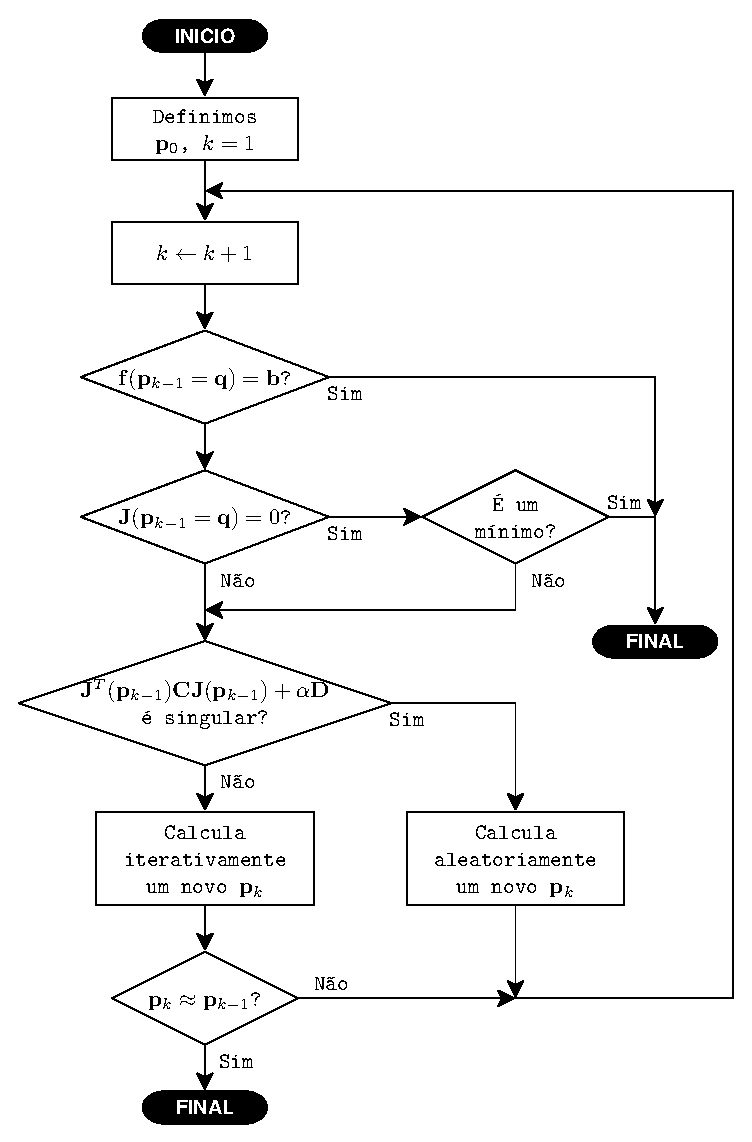
\includegraphics[width=0.75\textwidth]{chapters/minimization-fx/fluxo2.eps}
        \caption{Diagrama de fluxo da solução iterativa para achar um mínimo, seguindo a Prova \ref{proof:theo:minfxbCfxbaxqd}.}
        \label{fig:fluxo2}
\end{figure}

%%%%%%%%%%%%%%%%%%%%%%%%%%%%%%%%%%%%%%%%%%%%%%%%%%%%%%%%%%%%%%%%%%%%%%%%%%%%%%%%%%%%%%%
%%%%%%%%%%%%%%%%%%%%%%%%%%%%%%%%%%%%%%%%%%%%%%%%%%%%%%%%%%%%%%%%%%%%%%%%%%%%%%%%%%%%%%%
\begin{myproofT}[Prova do Teorema \ref{theo:minfxbCfxbaxoaxo}]\label{proof:theo:minfxbCfxbaxod}
Dados,
um escalar $\alpha\in \mathbb{R}$,
os vetores coluna $\VECTOR{x}\in \mathbb{R}^N$, 
$\VECTOR{x}_{last}\in \mathbb{R}^N$ e
$\VECTOR{b}\in \mathbb{R}^M$,  
uma função $\VECTOR{f}:\mathbb{R}^{N} \rightarrow \mathbb{R}^{M}$, 
as matrizes diagonais $\MATRIX{C} \in \mathbb{R}^{M\times M}$ e $\MATRIX{D} \in \mathbb{R}^{N\times N}$, e 
definida a Eq. (\ref{eq:proof:minfxbCfxbaxod0}),
\begin{equation}\label{eq:proof:minfxbCfxbaxod0}
e(\VECTOR{x})=||\VECTOR{f}(\VECTOR{x})-\VECTOR{b}||_{\MATRIX{C}}^2+\alpha||\VECTOR{x}-\VECTOR{x}_{last}||_{\MATRIX{D}}^2,
\end{equation}
tendo em consideração que $\VECTOR{x}_{last}$ é uma constante equivalente a $\VECTOR{x}_{k-1}$
numa busca iterativa ou equivalente a $\VECTOR{p}$, 
se decidimos usar uma aproximação linear ao redor de $\VECTOR{p}$ em $\VECTOR{f}(\VECTOR{x})$; 
é dizer, o segundo somando na Eq. (\ref{eq:proof:minfxbCfxbaxod0}) 
procura minimizar $||\VECTOR{x}_{k}-\VECTOR{x}_{k-1}||_{\MATRIX{D}}^2$.

Sabemos que para achar o ponto $\VECTOR{\hat{x}}$ que gere o menor valor de $e(\VECTOR{\hat{x}})$, é aplicado
o critério que um ponto de inflexão $\VECTOR{x}^+$; é dizer, um máximo, um mínimo ou um ponto de sela, pode ser achado quando 
$\frac{\partial e(\VECTOR{x}^+)}{\partial \VECTOR{x} }=[0~ 0~ \hdots~ 0 ]^{\transpose}$ (ver Figura \ref{fig:ex0b});
assim, usando o Teorema \ref{theo:derfxbCfxb0} e o Corolário \ref{coro:derAxbAxb2} obtemos que
\begin{equation}\label{eq:proof:minfxbCfxbaxod1exact2}
2 \MATRIX{J}(\VECTOR{x}^+)^{\transpose}\MATRIX{C}\left[ \VECTOR{f}(\VECTOR{x}^+)-\VECTOR{b} \right] +
2 \alpha\MATRIX{D}\left[\VECTOR{x}^+-\VECTOR{x}_{last}\right]
=
\frac{\partial e(\VECTOR{x}^+)}{\partial \VECTOR{x} }=[0~ 0~ \hdots~ 0 ]^{\transpose}.
\end{equation}
Da Eq. (\ref{eq:proof:minfxbCfxbaxod1exact2}) observamos, 
que podemos achar um ponto de inflexão $\VECTOR{x}^+=\VECTOR{x}_{last}$
em $e(\VECTOR{x}_{last})$ se 
$\MATRIX{J}(\VECTOR{x}_{last})  = \MATRIX{0}$ ou um mínimo geral se $\VECTOR{f}(\VECTOR{x}_{last})=\VECTOR{b}$,
caso contrario, 
se nenhuma destas possibilidades são cumpridas devemos aplicar outros critérios para achar os pontos de inflexão.



Assim, procurando outros critérios, podemos igualar $\VECTOR{x}_{last}\equiv \VECTOR{p}$ e 
realizar uma aproximação linear de $\VECTOR{f}(\VECTOR{x})$ em $e(\VECTOR{x})$
ao redor do ponto $\VECTOR{p}$ usando a \hyperref[def:taylor]{\textbf{serie de Taylor}},
de modo que a Eq. (\ref{eq:proof:minfxbCfxbaxod0}) pode ficar expressada como
\begin{equation}\label{eq:proof:minfxbCfxbaxod0alphaxqDapprox}
e(\VECTOR{x}) \approx e_{\VECTOR{p}}(\VECTOR{x})  \equiv 
||\MATRIX{J}(\VECTOR{p})[\VECTOR{x}-\VECTOR{p}]-[\VECTOR{b}-\VECTOR{f}(\VECTOR{p})]||_{\MATRIX{C}}^2+
\alpha||\VECTOR{x}-\VECTOR{p}||_{\MATRIX{D}}^2,
\end{equation}
onde $\MATRIX{J}(\VECTOR{p})$ representa a \hyperref[def:jacobian]{\textbf{matriz Jacobiana}} 
de $\VECTOR{f}(\VECTOR{x})$ avaliada no ponto $\VECTOR{p}$.
Assim, usando o resultado da Prova \ref{proof:theo:minAxbCAxbalphaxqD} na Eq. (\ref{eq:proof:minfxbCfxbaxod0alphaxqDapprox}), 
onde se aplica que $\frac{\partial e_{\VECTOR{p}}(\VECTOR{x}^*)}{\partial \VECTOR{x} }=\VECTOR{0}$,
podemos concluir que um ponto $\VECTOR{x}^*$ que é 
um mínimo da aproximação linear feita em $e(\VECTOR{x})$ ao redor do ponto $\VECTOR{p}$,
pode ser achado como,
\begin{equation}\label{eq:proof:minfxbCfxbaxod2}
\VECTOR{x}^* \approx \VECTOR{p} +
\left[ \MATRIX{J}(\VECTOR{p})^{\transpose}\MATRIX{C} \MATRIX{J}(\VECTOR{p})+\alpha \MATRIX{D} \right]^{-1}
\MATRIX{J}(\VECTOR{p})^{\transpose}\MATRIX{C} \left[\VECTOR{b}-\VECTOR{f}(\VECTOR{p})\right].
\end{equation}

Desta equação podemos tirar a seguintes conclusões:
\begin{itemize}

\item Observamos que a posição $\VECTOR{p}$ é corregida para ficar próximo à posição $\VECTOR{x}^*$, 
que é o valor mínimo na aproximação linear ao redor de $\VECTOR{p}$;
pelo que se deduz que a Eq. (\ref{eq:proof:minfxbCfxbaxod2})
pode ser usada para procurar aproximações de pontos mínimos $\VECTOR{\hat{x}}$ em $e(\VECTOR{x})$ desde a posição $\VECTOR{p}$,
ou pelo menos aproximações de novas posições em caminhos numa direção descendente de $e(\VECTOR{x})$.

\item A Eq. (\ref{eq:proof:minfxbCfxbaxod2}) é satisfeita 
com $\VECTOR{x}^* \approx \VECTOR{p}$ se acharmos um  
ponto $\VECTOR{p}$ onde  $\VECTOR{b} \approx \VECTOR{f}(\VECTOR{p}\approx \VECTOR{x}_{last})$; 
é dizer um mínimo global de $e(\VECTOR{x})$ em $\VECTOR{p}$, como pode ser visto na Figura \ref{fig:ex0a}. 

\item Se reescrevemos a Eq. (\ref{eq:proof:minfxbCfxbaxod2}) usando o Teorema \ref{theo:derfxbCfxb0}
e o Corolário \ref{coro:derAxbAxb2},
obtemos
\begin{equation}\label{eq:proof:minfxbCfxbaxod2ea1}
\VECTOR{x}^* \approx \VECTOR{p} -
0.5 \left[ \MATRIX{J}(\VECTOR{p})^{\transpose}\MATRIX{C} \MATRIX{J}(\VECTOR{p})+\alpha \MATRIX{D} \right]^{-1}
\frac{\partial e(\VECTOR{p})}{\partial \VECTOR{x} },
\end{equation}
onde a Eq. (\ref{eq:proof:minfxbCfxbaxod2ea1}) é satisfeita 
com $\VECTOR{x}^* \approx \VECTOR{p}$
se acharmos um  ponto $\VECTOR{p}$ onde  
$\frac{\partial e(\VECTOR{p})}{\partial \VECTOR{x} }\approx \VECTOR{0}$; 
é dizer $\VECTOR{p}$ é um ponto de inflexão de $e(\VECTOR{x})$, como pode ser visto na Figura \ref{fig:ex0b}.
Porem, dado que a equação avança desde $\VECTOR{p}$ na direção de um mínimo $\VECTOR{x}^*$, 
mesmo que nos pontos de inflexão correspondentes a máximos ou pontos de sela,
encontremos valores de $\VECTOR{p}$ próximos a $\VECTOR{x}^*$,
 estes casos serão pouco estáveis pois
a correção da posição $\VECTOR{p}$ será na direção de um mínimo e não do máximo.

\item Se modificamos a Eq. (\ref{eq:proof:minfxbCfxbaxod2}), e escolhemos um ponto  
$\VECTOR{p}_0$ que consideremos próximo ao ponto $\VECTOR{\hat{x}}$ que minimiza $e(\VECTOR{\hat{x}})$,
podemos achar iterativamente aproximações lineares $\VECTOR{x}^*$ cada vez mais próximos a  $\VECTOR{\hat{x}}$,
se usamos a seguinte equação iterativa,
\begin{equation}\label{eq:proof:minfxbCfxbaxod3b}
\VECTOR{p}_{k} \leftarrow \VECTOR{p}_{k-1} -
\left[ \MATRIX{J}(\VECTOR{p}_{k-1})^{\transpose}\MATRIX{C} \MATRIX{J}(\VECTOR{p}_{k-1}) +\alpha \MATRIX{D}\right]^{-1}
\MATRIX{J}(\VECTOR{p}_{k-1})^{\transpose}\MATRIX{C} \left[\VECTOR{f}(\VECTOR{p}_{k-1})-\VECTOR{b}\right],
\end{equation}
onde se inicia desde um $\VECTOR{p}_{0}$ 
ate que exista uma tendencia prolongada onde se observe que $\VECTOR{p}_{k}$ é muito próximo a $\VECTOR{p}_{k-1}$,
momento no qual declaramos que $\VECTOR{\hat{x}} \approx \VECTOR{p}_{k}$.
Disto também se deduz que o erro a minimizar em cada iteração será diferente e influenciado pelo valor do ponto $\VECTOR{p}_{k-1}$,
\begin{equation}
e_{k-1}(\VECTOR{x})  \equiv 
||\VECTOR{f}(\VECTOR{x})-\VECTOR{b}||_{\MATRIX{C}}^2+
\alpha||\VECTOR{x}-\VECTOR{p}_{k-1}||_{\MATRIX{D}}^2
\end{equation}
\item Como foi visto na Figura  \ref{fig:ex0b},
pode existir um mínimo global $\VECTOR{\hat{x}}$ de $e(\VECTOR{\hat{x}}) > 0$.
Isto nos restringe a que no uso da Eq. (\ref{eq:proof:minfxbCfxb3a}),
nosso critério principal para estabelecer o final do cálculo iterativo,
deve ser a tendencia na  proximidade entre $\VECTOR{p}_{k}$ e $\VECTOR{p}_{k-1}$ 
e não o valor de $e(\VECTOR{x}_k)$.
\end{itemize}~

Um diagrama completo resumindo todas estas conclusões pode ser visto na Figura \ref{fig:fluxo3}.
\end{myproofT}
\begin{figure}[!h]
     \centering
         \includegraphics[width=0.75\textwidth]{chapters/minimization-fx/fluxo3.eps}
        \caption{Diagrama de fluxo da solução iterativa para achar um mínimo, seguindo a Prova \ref{proof:theo:minfxbCfxbaxod}.}
        \label{fig:fluxo3}
\end{figure}


\begin{comment}
%%%%%%%%%%%%%%%%%%%%%%%%%%%%%%%%%%%%%%%%%%%%%%%%%%%%%%%%%%%%%%%%%%%%%%%%%%%%%%%%%%%%%%%
\section{Minimização de $\frac{||\VECTOR{f}(\VECTOR{x})-\VECTOR{b}||^2}{||\VECTOR{b}||^2}$
$+\alpha\frac{||\VECTOR{x}-\VECTOR{q}||^2}{||\VECTOR{q}||^2}$  
}
\textcolor{red}{Inventado por mi ..., creo.}
%%%%%%%%%%%%%%%%%%%%%%%%%%%%%%%%%%%%%%%%%%%%%%%%%%%%%%%%%%%%%%%%%%%%%%%%%%%%%%%%%%%%%%%
\section{Minimização de $||\VECTOR{f}(\VECTOR{x})-\VECTOR{b}||_{\MATRIX{B}^{-2}}^2$
$+\alpha||\VECTOR{x}-\VECTOR{q}||_{\MATRIX{Q}^{-2}}^2$  
}
\textcolor{red}{Inventado por mi ..., creo Nenhun valor de $\VECTOR{b}$ ou $\VECTOR{q}$ pode ser zero.}
\end{comment}


\chapterimage{chapter_head_2.pdf} % Chapter heading image

\chapter{Minimização do erro em funções: $\mathbb{R}$ $\rightarrow$ $\mathbb{R}$}

%%%%%%%%%%%%%%%%%%%%%%%%%%%%%%%%%%%%%%%%%%%%%%%%%%%%%%%%%%%%%%%%%%%%%%%%%%%%%%%%%%%%%%%
\section{\textcolor{blue}{Minimização de $||h(x)-a||^2$}} 

\begin{theorem}[Solução iterativa]\label{theo:minhxhx}
Dados,
um escalar $x \in \mathbb{R}$, 
um escalar $a \in \mathbb{R}$,  
uma função $h:\mathbb{R} \rightarrow \mathbb{R}$, e 
definida a Eq. (\ref{eq:minhxhx1}),
\begin{equation}\label{eq:minhxhx1}
e(x)=||h(x)-a||^2.
\end{equation}
Se desejamos ter o valor $\hat{x}$ que minimiza o escalar $e(\hat{x})$,
este valor pode ser achado usando iterativamente a Eq. (\ref{eq:minhxhx2}),
\begin{equation}\label{eq:minhxhx2}
x_{k+1} \leftarrow x_k+
\frac{ a-h(x_k)}{h'(x_k)}
\end{equation}
Onde  $h'(x)=\frac{\partial h(x)}{\partial x}$. A busca iterativa é considerada 
falida quando se atinge $h'(x_k) = 0$.
Assim, $\hat{x}$ pode ser achado iniciando a Eq. (\ref{eq:minhxhx2}) desde um $x_{0}$ qualquer, ate que $x_{k}$ seja muito próximo a $x_{k+1}$,
onde se declara que $\hat{x} \approx x_{k+1}$; porem deve ser corroborado
que esse ponto tratasse de um máximo ou mínimo usando algum método, por exemplo estudando o comportamento 
de $e(x)$ ou analisando  $\frac{\partial^2 e(x)}{\partial x^2}$ avaliada em $\hat{x}$.

\textcolor{red}{Esta forma de iterar tambem e conhecida como metodo de Newton.}

\FALTAPROVA
A demostração pode ser vista na Prova \ref{proof:theo:minhxhx}.
\end{theorem}

%%%%%%%%%%%%%%%%%%%%%%%%%%%%%%%%%%%%%%%%%%%%%%%%%%%%%%%%%%%%%%%%%%%%%%%%%%%%%%%%%%%%%%%
\section{\textcolor{blue}{Minimização de $||h(x)-a||^2+\alpha ||x-b||^2$}}

\begin{theorem}[Solução iterativa]\label{theo:minhxhxxbxb}
Dados,
um escalar $\alpha \in \mathbb{R} | \alpha > 0$, 
um escalar $x \in \mathbb{R}$, 
um escalar $a \in \mathbb{R}$,  
uma função $h:\mathbb{R} \rightarrow \mathbb{R}$, e 
definida a Eq. (\ref{eq:minhxhxxbxb1}),
\begin{equation}\label{eq:minhxhxxbxb1}
e(x)=||h(x)-a||^2+\alpha ||x-b||^2.
\end{equation}
Se desejamos ter o valor $\hat{x}$ que minimiza o escalar $e(\hat{x})$,
este valor pode ser achado usando iterativamente a Eq. (\ref{eq:minhxhxxbxb2}),
\begin{equation}\label{eq:minhxhxxbxb2}
x_{k+1} \leftarrow x_k+
\frac{ h'(x_k) \left[a-h(x_k)\right]-\alpha\left[ x_k-b\right]}{\left[h'(x_k)\right]^2+\alpha}
\end{equation}
Onde  $h'(x)=\frac{\partial h(x)}{\partial x}$.
Assim, $\hat{x}$ pode ser achado iniciando a Eq. (\ref{eq:minhxhxxbxb2}) desde um $x_{0}$ qualquer, ate que $x_{k}$ seja muito próximo a $x_{k+1}$,
onde se declara que $\hat{x} \approx x_{k+1}$; porem deve ser corroborado
que esse ponto tratasse de um máximo ou mínimo usando algum método, por exemplo estudando o comportamento 
de $e(x)$ ou analisando  $\frac{\partial^2 e(x)}{\partial x^2}$ avaliada em $\hat{x}$.

\FALTAPROVA
A demostração pode ser vista na Prova \ref{proof:theo:minhxhxxbxb}.
\end{theorem}

%%%%%%%%%%%%%%%%%%%%%%%%%%%%%%%%%%%%%%%%%%%%%%%%%%%%%%%%%%%%%%%%%%%%%%%%%%%%%%%%%%%%%%%
\section{\textcolor{blue}{Minimização de $||h(x)-a||^2+\alpha ||x-x_{old}||^2$}}

\begin{theorem}[Solução iterativa]\label{theo:minhxhxxoxo}
Dados,
um escalar $\alpha \in \mathbb{R} | \alpha > 0$, 
um escalar $x \in \mathbb{R}$, 
um escalar $a \in \mathbb{R}$,  
uma função $h:\mathbb{R} \rightarrow \mathbb{R}$, e 
definida a Eq. (\ref{eq:minhxhxxoxo1}),
\begin{equation}\label{eq:minhxhxxoxo1}
e(x)=||h(x)-a||^2+\alpha ||x-x_{old}||^2.
\end{equation}
Se desejamos ter o valor $\hat{x}$ que minimiza o escalar $e(\hat{x})$,
este valor pode ser achado usando iterativamente a Eq. (\ref{eq:minhxhxxoxo2}),
\begin{equation}\label{eq:minhxhxxoxo2}
x_{k+1} \leftarrow x_k+
\frac{ h'(x_k) \left[a-h(x_k)\right] }{\left[h'(x_k)\right]^2+\alpha}
\end{equation}
Onde  $h'(x)=\frac{\partial h(x)}{\partial x}$.
Assim, $\hat{x}$ pode ser achado iniciando a Eq. (\ref{eq:minhxhxxoxo2}) desde um $x_{0}$ qualquer, ate que $x_{k}$ seja muito próximo a $x_{k+1}$,
onde se declara que $\hat{x} \approx x_{k+1}$; porem deve ser corroborado
que esse ponto tratasse de um máximo ou mínimo usando algum método, por exemplo estudando o comportamento 
de $e(x)$ ou analisando  $\frac{\partial^2 e(x)}{\partial x^2}$ avaliada em $\hat{x}$.

\FALTAPROVA
A demostração pode ser vista na Prova \ref{proof:theo:minhxhxxoxo}.
\end{theorem}




%----------------------------------------------------------------------------------------
%	PART
%----------------------------------------------------------------------------------------
\part{Aplicações: não lineares ou problemas inversos}
% CHAPTER  
\chapterimage{chapter_roots.pdf} % Chapter heading image

\chapter{Raízes de funções}


%%%%%%%%%%%%%%%%%%%%%%%%%%%%%%%%%%%%%%%%%%%%%%%%%%%%%%%%%%%%%%%%%%%%%%%%%%%%%%%%%%%%%%%
\section{ Método de Newton para funções $h(x)$: $\mathbb{R}$ $\rightarrow$ $\mathbb{R}$ }

\begin{theorem}[Solução iterativa]\label{theo:rootshx}
~\\
\begin{minipage}{0.20\textwidth}
\centering
\includegraphics[width=0.9\linewidth]{chapters/roots/roots1.eps} 
\end{minipage}
\begin{minipage}{0.8\textwidth}
Dados
um escalar $\delta \in \mathbb{R}_+$, 
um escalar $x \in \mathbb{R}$, 
uma função $h:\mathbb{R} \rightarrow \mathbb{R}$, e 
conhecida a validade da Eq. (\ref{eq:rootshx1}),
\begin{equation}\label{eq:rootshx1}
0=h(x);
\end{equation}
se desejarmos ter o valor $x=\hat{x}$ que cumpra a Eq. (\ref{eq:rootshx1}),
podemos usar iterativamente a Eq. (\ref{eq:rootshx2}),
na qual $h'(x)\equiv \frac{d h(x)}{d x}$,
\end{minipage}

\begin{equation}\label{eq:rootshx2}
x_{k} \leftarrow x_{k-1}-\frac{ h(x_{k-1})}{h'(x_{k-1})}.
\end{equation}
Assim, $\hat{x}$ pode ser achado\footnote{A 
demonstração pode ser vista na Prova \ref{proof:theo:rootshx}.} 
iniciando a Eq. (\ref{eq:rootshx2}) desde um 
$x_{0}$ qualquer, realizando cálculos $x_{k}$ iterativamente  
até\footnote{Sendo $\delta$ um valor pequeno próximo a zero.} que $||h(x_k)||<\delta$,
nesse caso se declara que $\hat{x}=x_k$.

\textbf{Considerações:}
\begin{itemize} 
\item Se $h'(x_{k-1})\approx 0$, então estamos perto de um ponto de inflexão 
(máximo, mínimo ou ponto de sela) em $x_{k-1}$. Nesses pontos a Eq. (\ref{eq:rootshx2}): 
\begin{itemize}
\item Diverge quando se cumpre que $h(x_{k-1})\neq 0$, ou
\item Converge\footnote{A demonstração pode ser vista na Prova \ref{proof:theo:cont:rootshx}.} 
se $h(x_{k-1}) = 0$ e se verifica que $h(x)$ pode ser representado 
mediante uma \hyperref[def:taylor]{\textbf{série de Taylor}} ao redor de $x_{k-1}$, 
 pois indica que $\lim_{x\rightarrow x_{k-1}}  h(x)/h'(x)$ é finito.
\end{itemize}
\item Uma sugestão do procedimento para a busca de uma raiz pode ser vista no diagrama de fluxo
mostrado na Figura \ref{fig:fluxorhx1}. 
\end{itemize}
\end{theorem}

\begin{figure}[!h]
     \centering
         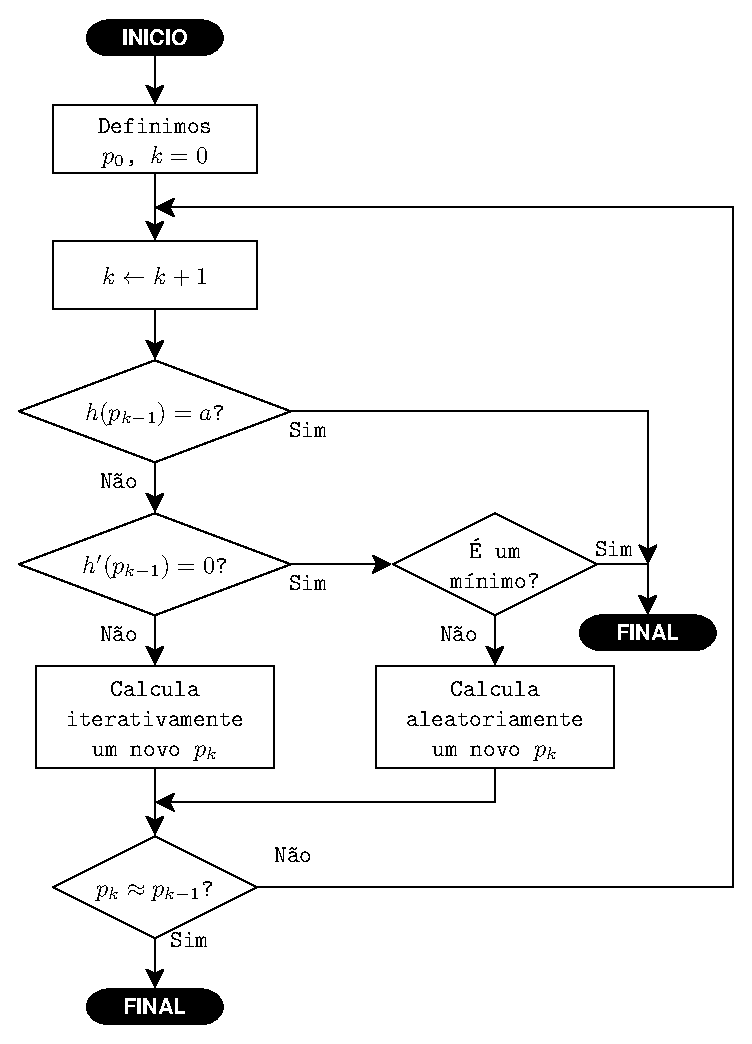
\includegraphics[width=0.75\textwidth]{chapters/roots/fluxo1.eps}
        \caption{Diagrama de fluxo da solução iterativa para achar uma raiz, seguindo o teorema \ref{theo:rootshx}.}
        \label{fig:fluxorhx1}
\end{figure}

\newpage
%%%%%%%%%%%%%%%%%%%%%%%%%%%%%%%%%%%%%%%%%%%%%%%%%%%%%%%%%%%%%%%%%%%%%%%%%%%%%%%%
\subsection{Exemplos de busca de raízes pelo método de Newton}


\begin{example}\label{ex:rootshx1}
Conhecida uma função $h(x)=x(x^2-1)+1$, e um escalar $\delta=10^{-3}$;
usando o Teorema \ref{theo:rootshx}, 
achar um valor $x=\hat{x}$ que cumpra $||h(x)||<\delta$.
Podemos ver as respostas a esse exemplo na Solução \ref{sol:rootshx1} e \ref{sol:rootshx2}.
\end{example}
\begin{SolutionT}[Relativa ao Exemplo \ref{ex:rootshx1} (Diverge):]\label{sol:rootshx1}
 A Fig. \ref{fig:rootsNcasesa} nos mostra o processo de busca das raízes de $h(x)$. 
A busca inicia em $x_0=-0.3$, 
todos os valores $x_{k}$ podem ser vistos na
Tabela \ref{tab:rootsNcases1}. 
Neste caso, a busca iterativa indicada pela Eq. (\ref{eq:rootshx2}) 
diverge para valores próximos a $x_m=\frac{\sqrt{3}}{3}\approx 0.57735$,
que é um mínimo local de $h(x)$; quer dizer, $h'(x_m)\approx 0$ e $h(x_m)\neq 0$.
É fácil de observar que neste caso se produz 
uma espécie de efeito sanfona, no qual $x_{k}$ se aproxima ao mínimo local em $h(x)$, e quando 
está próximo desse valor, a busca volta a divergir a um ponto medianamente distante.
\end{SolutionT}

\begin{figure}[!h]
    \centering
    \begin{subfigure}[b]{0.49\textwidth}
        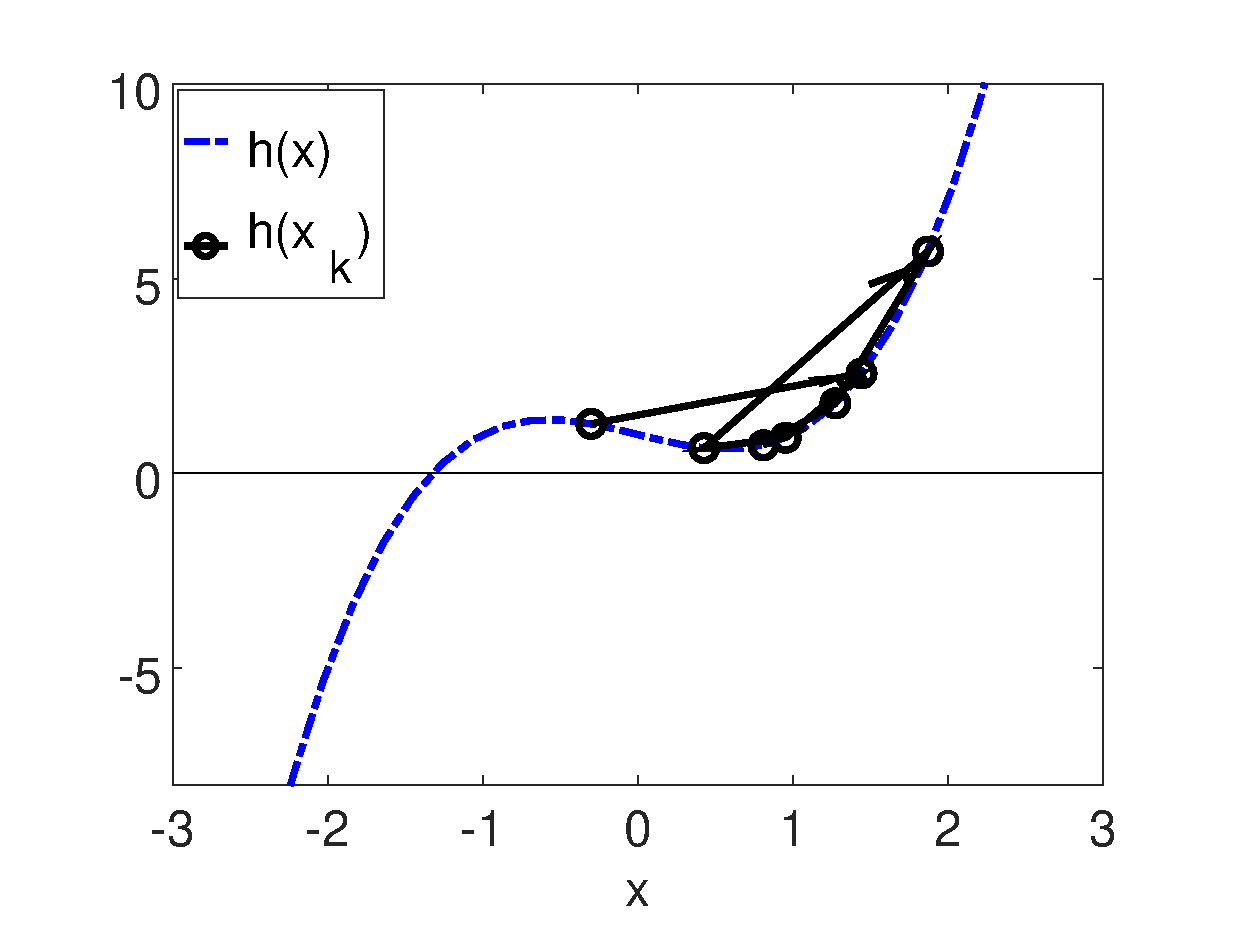
\includegraphics[width=\textwidth]{chapters/roots/mfiles/hx/minimizando_hx_1.eps}
        \caption{As iterações divergem ao redor da amostra $x_m$ em que $h'(x_m)\approx 0$ e $h(x_m)\neq 0$.}
        \label{fig:rootsNcasesa}
    \end{subfigure}
    ~ %add desired spacing between images, e. g. ~, \quad, \qquad, \hfill etc. 
      %(or a blank line to force the subfigure onto a new line)
    \begin{subfigure}[b]{0.49\textwidth}
        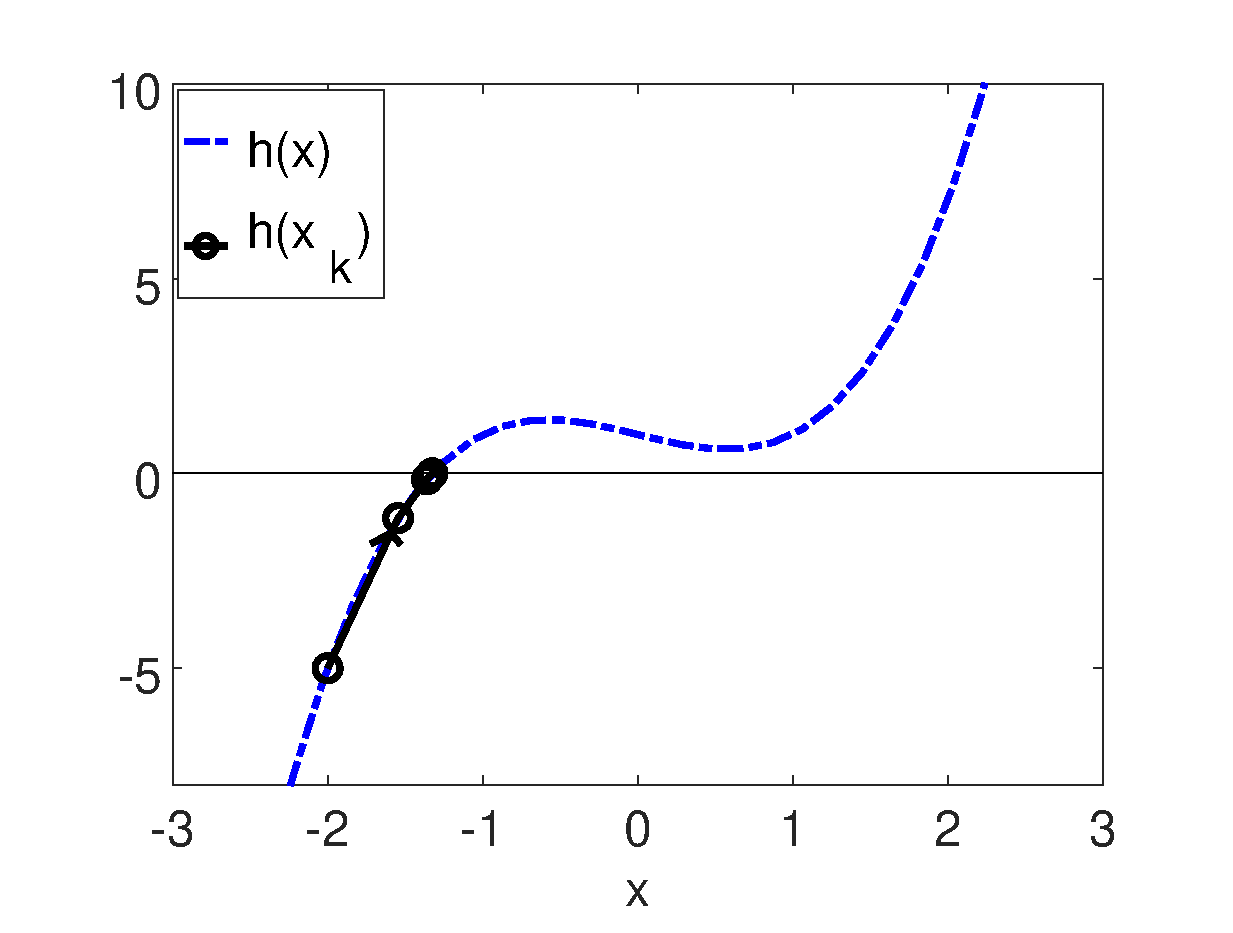
\includegraphics[width=\textwidth]{chapters/roots/mfiles/hx/minimizando_hx_2.eps}
        \caption{As iterações convergem em $\hat{x}$, no qual $h(\hat{x})\approx 0$ e $h'(x_m)\neq 0$.}
        \label{fig:rootsNcasesb}
    \end{subfigure}
    \caption{Comportamento da busca iterativa do Exemplo \ref{ex:rootshx1}}
    \label{fig:rootsNcases}
\end{figure}

\begin{table}[!h]
\centering
\begin{tabular}{|l|l|l|l|l|l|l|l|}
\hline
$k$      & 0 & 1 & 2 & 3 & 4 & 5 & 6\\ \hline
$x_k$    & -0.30000 & 1.44384 & 0.95543 & 0.42813 & 1.87298 & 1.27476 & 0.81109 \\ \hline
$||h(x_k)||$ & 1.27300 & 2.56607 & 0.91673 & 0.65034 & 5.69758 & 1.79676 & 0.72250 \\ \hline
\end{tabular}
\caption{Resposta iterativa do Exemplo \ref{ex:rootshx1}.}
\label{tab:rootsNcases1}
\end{table}

\begin{SolutionT}[Relativa ao Exemplo \ref{ex:rootshx1} (Converge):]\label{sol:rootshx2}
A Fig. \ref{fig:rootsNcasesb} nos mostra o processo de busca de uma raiz de $h(x)$. 
A busca inicia em $x_0=-2.0$,
 todos os valores $x_{k}$ podem ser vistos na Tabela \ref{tab:rootsNcases2}. 
Neste caso, a busca iterativa indicada pela Eq. (\ref{eq:rootshx2}) converge 
em $x_4\approx 0$ com $||h(x_4)||<\delta$ que corresponde a uma raiz de $h(x)$.
\end{SolutionT}

\begin{table}[!h]
\centering
\begin{tabular}{|l|l|l|l|l|l|}
\hline
$k$      & 0 & 1 & 2 & 3 & 4 \\ \hline
$x_k$    & -2.0000 & -1.5455 & -1.3596 & -1.3258 & -1.3247 \\ \hline
$||h(x_k)||$ & 5.0000 &  1.1458 & 1.5370e-01 & 4.6249e-03 & 4.6577e-06 \\ \hline
\end{tabular}
\caption{Resposta iterativa do Exemplo \ref{ex:rootshx1}.}
\label{tab:rootsNcases2}
\end{table}

\begin{example}\label{ex:rootshx2}
Conhecida uma função $h(x)=x(x^2-1)+2\frac{\sqrt{3}}{9}$ e um escalar $\delta=2~10^{-5}$;
usando o Teorema \ref{theo:rootshx},
achar o valor $x=\hat{x}$ que cumpra $||h(x)||<\delta$.
Podemos ver a resposta a este exemplo na Solução \ref{sol:rootshx3}.
\end{example}

\begin{SolutionT}[Relativa ao Exemplo \ref{ex:rootshx2} (Converge):]\label{sol:rootshx3}
A Fig. \ref{fig:rootsNcasesc} nos mostra o processo de busca de uma raiz de $h(x)$. 
A busca inicia em $x_0=-0.3$,
 todos os valores $x_{k}$ podem ser vistos na Tabela \ref{tab:rootsNcases3}. 
Neste caso, a busca iterativa indicada pela Eq. (\ref{eq:rootshx2}) converge 
em $x_4\approx 0$ com $||h(x_4)||<\delta$ que corresponde a uma raiz de $h(x)$.
Analiticamente podemos verificar que uma raiz pode ser achada em $x_m=\frac{\sqrt{3}}{3}\approx 0.57735$.
\end{SolutionT}

\begin{table}[!h]
\centering
\begin{tabular}{|l|l|l|l|l|l|}
\hline
$k$      & 0 & 1 & 2 & 3 & 4 \\ \hline
$x_k$    & -0.30000 & 0.60123 & 0.58937 & 0.58338 & 0.58037 \\ \hline
$||h(x_k)||$ & 6.5790e-01 & 1.0016e-03 & 2.5207e-04 & 6.3234e-05 & 1.5836e-05 \\ \hline
\end{tabular}
\caption{Resposta iterativa do Exemplo \ref{ex:rootshx1}.}
\label{tab:rootsNcases3}
\end{table}

    \begin{figure}[!h]
        \centering
        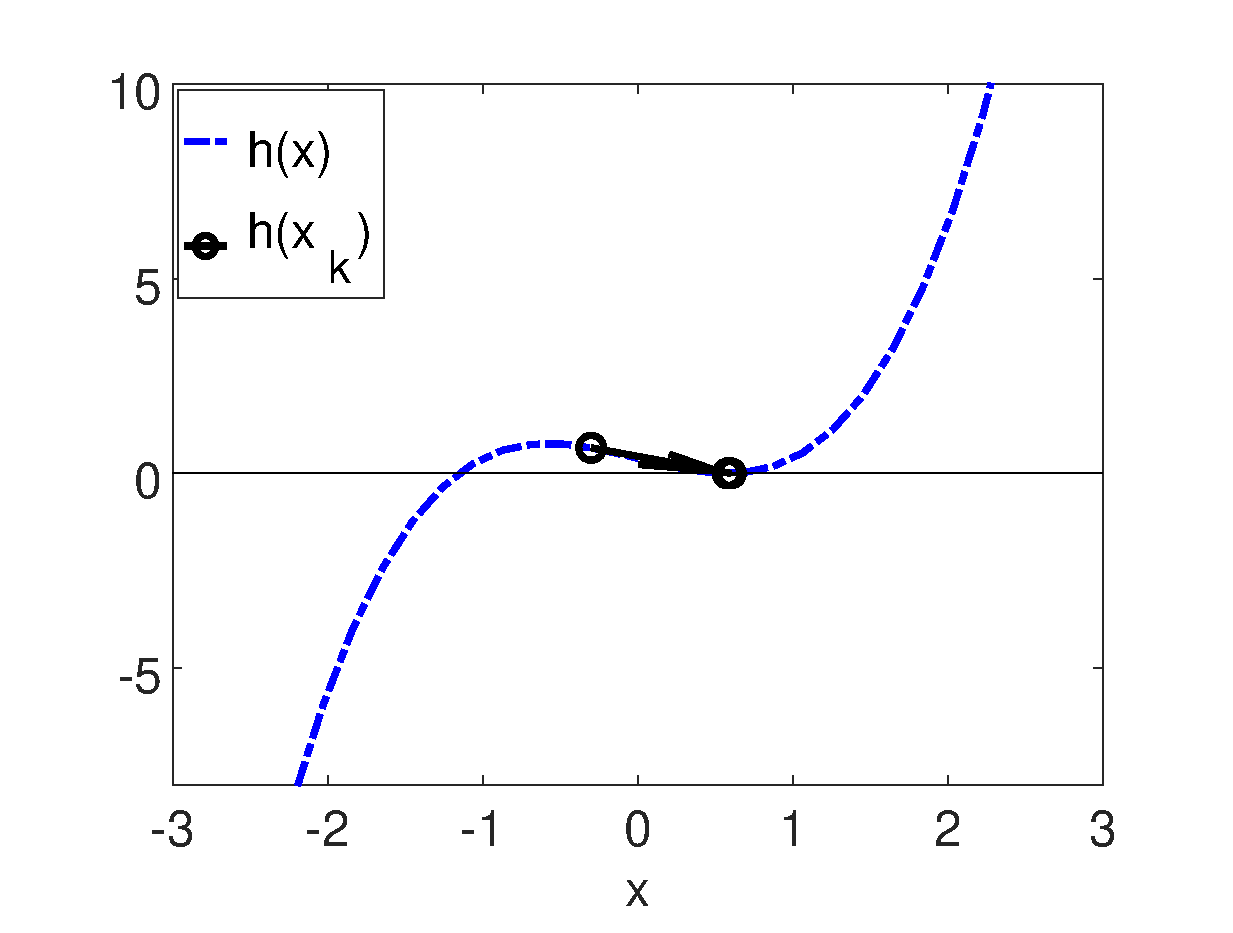
\includegraphics[width=0.49\textwidth]{chapters/roots/mfiles/hx2/minimizando_hx_1.eps}
        \caption{Resposta iterativa do Exemplo \ref{ex:rootshx2}, no qual $h'(x_m)\approx 0$ e $h(x_m)\approx 0$.}
        \label{fig:rootsNcasesc}
    \end{figure}



\newpage

%%%%%%%%%%%%%%%%%%%%%%%%%%%%%%%%%%%%%%%%%%%%%%%%%%%%%%%%%%%%%%%%%%%%%%%%%%%%%%%%%%%%%%%
\section{ Método mediante regularização para funções $h(x)$: $\mathbb{R}$ $\rightarrow$ $\mathbb{R}$ }

\begin{theorem}[Solução iterativa]\label{theo:rootshxreg}
~\\
\begin{minipage}{0.2\textwidth}
\centering
\includegraphics[width=0.95\linewidth]{chapters/roots/roots1.eps} 
\end{minipage}
\begin{minipage}{0.8\textwidth}
Dados,
um escalar $\delta \in \mathbb{R}$, 
um escalar $\alpha \in \mathbb{R}| \alpha>0$, 
um escalar $x \in \mathbb{R}$, 
uma função $h:\mathbb{R} \rightarrow \mathbb{R}$, e 
conhecida a validade da Eq. (\ref{eq:rootshxreg1}),
\begin{equation}\label{eq:rootshxreg1}
0=h(x);
\end{equation}
se desejamos ter o valor $x=\hat{x}$ que cumpra a Eq. (\ref{eq:rootshxreg1})
podemos usar iterativamente a Eq. (\ref{eq:rootshxreg2}),
onde  $h'(x)\equiv \frac{d h(x)}{d x}$,
\end{minipage}

\begin{equation}\label{eq:rootshxreg2}
x_{k} \leftarrow x_{k-1}-\frac{ h'(x_{k-1})h(x_{k-1})}{h'(x_{k-1})^2+\alpha}.
\end{equation}
Assim, $\hat{x}$ pode ser achado\footnote{A 
demostração pode ser vista na Prova \ref{proof:theo:rootshxreg}.} 
iniciando a Eq. (\ref{eq:rootshxreg2}) desde um 
$x_{0}$ qualquer, realizando cálculos $x_{k}$ iterativamente  
ate\footnote{Sendo delta um valor pequeno próximo a zero.} que $||h(x_k)||<\delta$
onde se declara que $\hat{x}=x_k$.

\textbf{Considerações:}
\begin{itemize} 
\item Se $h'(x_{k-1})\approx 0$ indica que estamos perto de um ponto de inflexão 
(máximo, mínimo ou ponto de sela) em $x_{k-1}$. Se neste ponto a Eq. (\ref{eq:rootshxreg2})
converge com valores $x_k\approx x_{k-1}\approx x_{k-2}\approx ...$ e verificamos que $||h(x_{k-1})||>\delta$,
devemos pular aleatoriamente a um novo ponto $x_k$ pois estamos atrapados num mínimo local de $h(x)$.  
\item Uma sugestão do procedimento para a busca de uma raiz pode ser vista no diagrama de fluxo
mostrado na Figura \ref{fig:fluxorhxreg3}. 
\end{itemize}
\end{theorem}

\begin{tcbattention}
\begin{itemize}
\item Uma vantagem do método da regularização em relação ao método de Newton,
é que em lugares onde $h'(x_{k-1})\approx 0$, a regularização converge a um mínimo local 
que facilmente podemos detetar. Em contrapartida,
com o método de newton podemos ficar temporalmente atrapados num mínimo local, porem este estado 
é mais difícil de detetar pois os valores de $x_k$ tendem a divergir para valores próximos ao mínimo.
Esta caraterística pode ser comparada nas Soluções \ref{sol:rootshx1} e \ref{sol:rootshxreg1}
\end{itemize}
\end{tcbattention}

\begin{figure}[!h]
     \centering
         \includegraphics[width=0.75\textwidth]{chapters/roots/fluxo3.eps}
        \caption{Diagrama de fluxo da solução iterativa para achar uma raiz, seguindo o teorema \ref{theo:rootshxreg}.}
        \label{fig:fluxorhxreg3}
\end{figure}

%%%%%%%%%%%%%%%%%%%%%%%%%%%%%%%%%%%%%%%%%%%%%%%%%%%%%%%%%%%%%%%%%%%%%%%%%%%%%%%%
\subsection{Exemplos de busca de raízes pelo método da regularização}


\begin{example}\label{ex:rootshxreg1}
Conhecida uma função $h(x)=x(x^2-1)+1$, e um escalar $\delta=10^{-3}$; usando o Teorema \ref{theo:rootshxreg},
achar o valor $x=\hat{x}$ que cumpra $||h(x)||<\delta$ usando o Teorema \ref{theo:rootshxreg}.
Podemos ver as respostas a este exemplo na Solução \ref{sol:rootshxreg1} e \ref{sol:rootshxreg2}.
\end{example}
\begin{SolutionT}[Relativa ao Exemplo \ref{ex:rootshxreg1} (Converge errado):]\label{sol:rootshxreg1}
 A Fig. \ref{fig:rootsRcasesa} nos mostra o processo de busca das raízes de $h(x)$. 
A busca inicia em $x_0=-0.3$, 
todos os valores $x_{k}$ podem ser vistos na
Tabela \ref{tab:rootsRcases1}. 
Neste caso a busca iterativa indicada pela Eq. (\ref{eq:rootshxreg2}) 
converge em $x_7=0.57812$, que é um valor próximo a $x_m=\frac{\sqrt{3}}{3}\approx 0.57735$,
que é um mínimo local de $h(x)$.
Porem dado que $||h(x_7)||=0.61510 >\delta$, observamos que estamos atrapados num mínimo local,
pelo que devemos fazer um pulo aleatório a um novo valor $x_8$
para tentar fugir deste mínimo local; por exemplo $x_8=-2.0$.
\end{SolutionT}

\begin{figure}[!h]
    \centering
    \begin{subfigure}[b]{0.49\textwidth}
        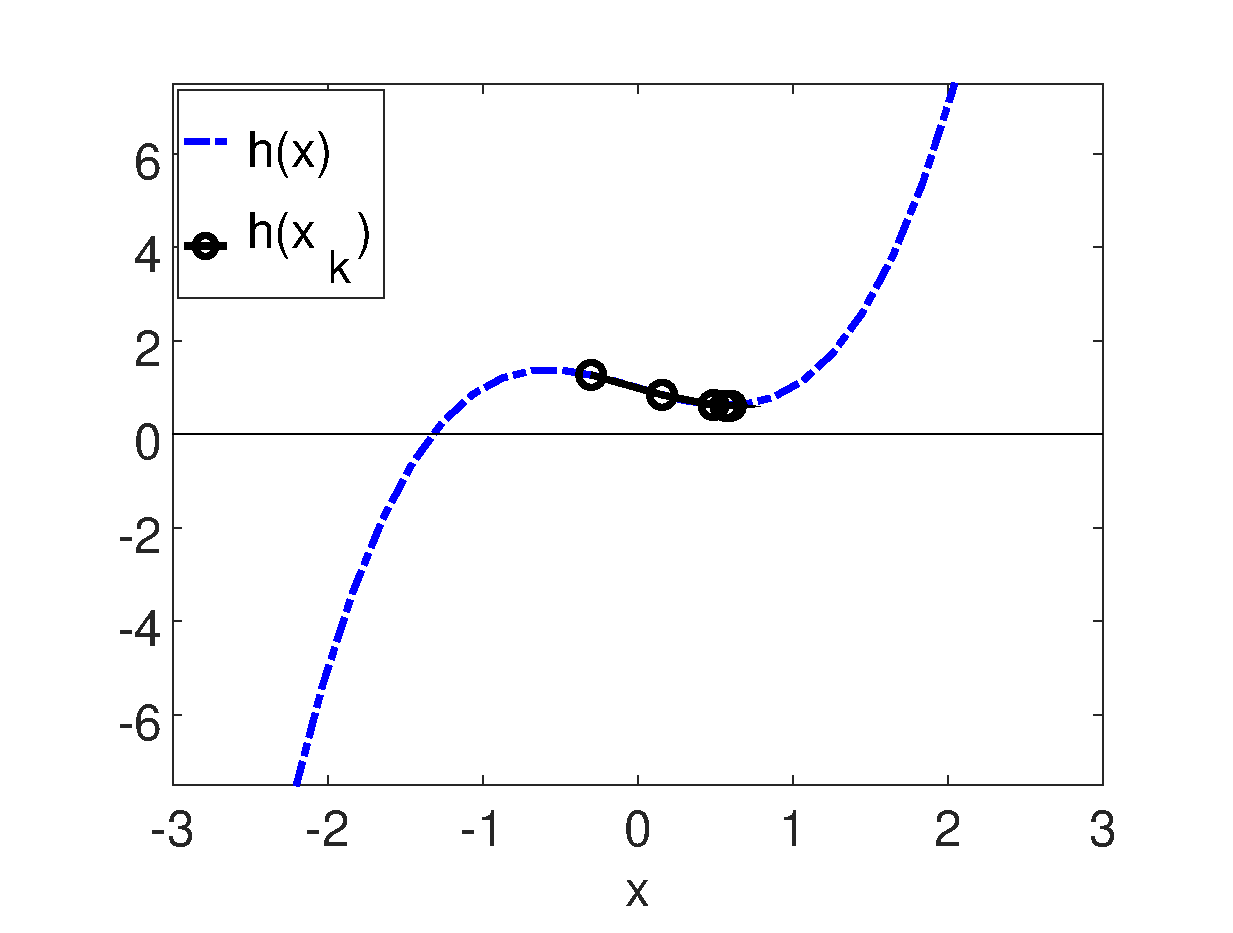
\includegraphics[width=\textwidth]{chapters/roots/mfiles/hx_a/minimizando_hx_a_1.eps}
        \caption{As iterações divergem ao redor de $x_m$, onde $h'(x_m)\approx 0$ e $h(x_m)\neq 0$.}
        \label{fig:rootsRcasesa}
    \end{subfigure}
    ~ %add desired spacing between images, e. g. ~, \quad, \qquad, \hfill etc. 
      %(or a blank line to force the subfigure onto a new line)
    \begin{subfigure}[b]{0.49\textwidth}
        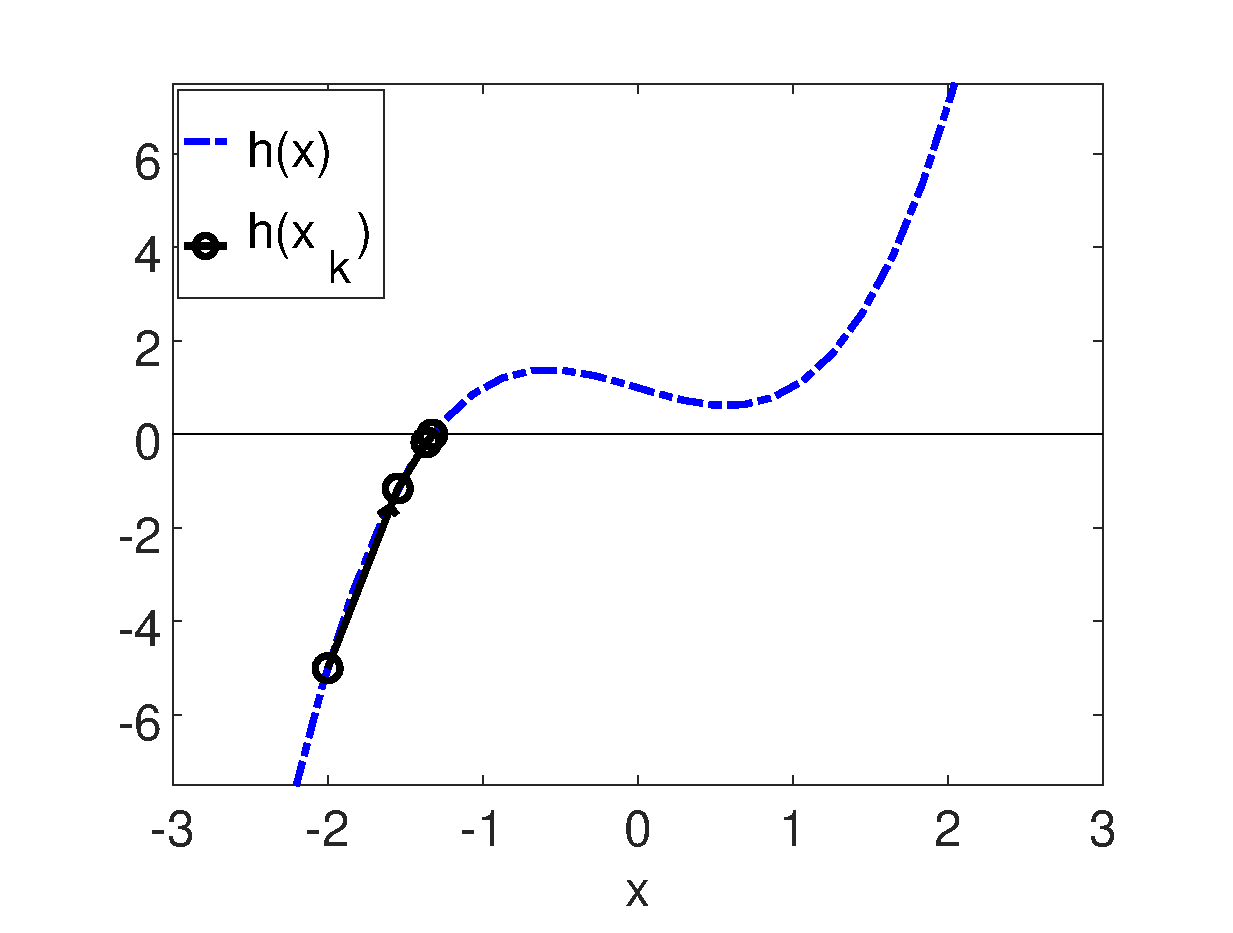
\includegraphics[width=\textwidth]{chapters/roots/mfiles/hx_a/minimizando_hx_a_2.eps}
        \caption{As iterações convergem em $\hat{x}$, onde $h(\hat{x})\approx 0$ e $h'(x_m)\neq 0$}
        \label{fig:rootsRcasesb}
    \end{subfigure}
    \caption{Comportamento da busca iterativa do Exemplo \ref{ex:rootshxreg1}}
    \label{fig:rootsRcases}
\end{figure}

\begin{table}[!h]
\centering
\begin{tabular}{|l|l|l|l|l|l|l|l|l|}
\hline
$k$      & 0 & 1 & 2 & 3 & 4 & 5 & 6 & 7\\ \hline
$x_k$    & -0.30000 & 0.15713 & 0.48972 & 0.60126 & 0.56670 & 0.58168 & 0.57551 & 0.57812 \\ \hline
$||h(x_k)||$ & 1.27300  & 0.84675 & 0.62773 & 0.61610 & 0.61530 & 0.61513 & 0.61511 & 0.61510 \\ \hline
\end{tabular}
\caption{Resposta iterativa do Exemplo \ref{ex:rootshxreg1}.}
\label{tab:rootsRcases1}
\end{table}

\begin{SolutionT}[Relativa ao Exemplo \ref{ex:rootshxreg1} (Converge errado):]\label{sol:rootshxreg2}
A Fig. \ref{fig:rootsRcasesb} nos mostra o processo de busca de uma raiz de $h(x)$. 
A busca inicia em $x_0=-2.0$,
 todos os valores $x_{k}$ podem ser vistos na Tabela \ref{tab:rootsRcases2}. 
Neste caso a busca iterativa indicada pela Eq. (\ref{eq:rootshxreg2}) converge 
em $\hat{x}\approx x_4 = -1.3248$ com $||h(x_4)||<\delta$ que corresponde a uma raiz de $h(x)$.
\end{SolutionT}

\begin{table}[!h]
\centering
\begin{tabular}{|l|l|l|l|l|l|}
\hline
$k$      & 0 & 1 & 2 & 3 & 4 \\ \hline
$x_k$    & -2.0000 & -1.5473 & -1.3626 & -1.3268 & -1.3248 \\ \hline
$||h(x_k)||$ & 5.0000e+00 & 1.1573e+00 & 1.6711e-01 & 9.0760e-03 & 2.5792e-04 \\ \hline
\end{tabular}
\caption{Resposta iterativa do Exemplo \ref{ex:rootshxreg1}.}
\label{tab:rootsRcases2}
\end{table}



\newpage
\section{Provas dos teoremas}
 
%%%%%%%%%%%%%%%%%%%%%%%%%%%%%%%%%%%%%%%%%%%%%%%%%%%%%%%%%%%%%%%%%%%%%%%%%%%%%%%%%%%%%%%
%%%%%%%%%%%%%%%%%%%%%%%%%%%%%%%%%%%%%%%%%%%%%%%%%%%%%%%%%%%%%%%%%%%%%%%%%%%%%%%%%%%%%%%
\begin{myproofT}[Prova do Teorema \ref{theo:rootshx}:]\label{proof:theo:rootshx}
Dados,
um escalar $\delta \in \mathbb{R}$, 
um escalar $x \in \mathbb{R}$, 
uma função $h:\mathbb{R} \rightarrow \mathbb{R}$, e 
conhecida a validade da Eq. (\ref{eq:prrof:rootshx1}),
\begin{equation}\label{eq:prrof:rootshx1}
0=h(x);
\end{equation}
se desejamos ter o valor $x=\hat{x}$ que cumpra que $||h(\hat{x})||<\delta$, 
é aplicado o critério mostrado no Teorema \ref{theo:minhxhx} onde se indica que uma forma de achar o 
$x=\hat{x}$ que minimize $e(x)=||h(x)||^2$ é mediante a seguinte equação iterativa.  
\begin{equation}\label{eq:prrof:rootshx1:2}
x_{k}=x_{k-1}-\frac{h(x_{k-1})}{h'(x_{k-1})};
\end{equation}

\end{myproofT}

\begin{myproofT}[Prova da continuidade de 
$h(x)/h'(x)$:]\label{proof:theo:cont:rootshx}
Conhecida uma função $h(x)$  diferenciável em $x=a$, ao menos ate a $n$-ésima derivada onde $h^(n)(a)\neq 0$.
Se $h(a)=0$ e $h'(a)=0$ o fator
\begin{equation}\label{eq:prrof:cont1}
F(x)=\frac{h(x)}{h'(x)}
\end{equation}
causa uma indeterminação de zero dividido por zero para $x=a$.
Para resolver este problema é aplicada a regra de l'Hôpital, de forma consecutiva,
sobre a Eq. (\ref{eq:prrof:cont1}), onde podemos afirmar
\begin{equation}\label{eq:prrof:cont2}
F(a)=\lim_{x\rightarrow a}\frac{h(x)}{h'(x)}=\frac{h^{(n-1)}(a)}{h^{(n)}(a)}
\end{equation}
onde $n$ é escolhido como o primeiro valor avaliado em $a$, 
onde se cumpra que $h^{(n)}(a)\neq 0$. 
Assim, podemos definir que os lugares onde $h(a)=0$ e $h'(a)=0$,
 tem um valor $F(a)\neq 0$,
se $h(x)$ tem ao menos uma derivada $n$-ésima em $x=a$ onde $h^{(n)}(a)\neq 0$.

Uma forma simples de expressar isto é indicar que $F(a)\neq 0$ sim é possível,
expressar $h(x)$ em \hyperref[def:taylor]{\textbf{serie de Taylor}} ao redor de $x=a$. 
\end{myproofT}

%%%%%%%%%%%%%%%%%%%%%%%%%%%%%%%%%%%%%%%%%%%%%%%%%%%%%%%%%%%%%%%%%%%%%%%%%%%%%%%%%%%%%%%
%%%%%%%%%%%%%%%%%%%%%%%%%%%%%%%%%%%%%%%%%%%%%%%%%%%%%%%%%%%%%%%%%%%%%%%%%%%%%%%%%%%%%%%
\begin{myproofT}[Prova do Teorema \ref{theo:rootshxreg}:]\label{proof:theo:rootshxreg}
Dados,
um escalar $\delta \in \mathbb{R}$, 
um escalar $x \in \mathbb{R}$, 
uma função $h:\mathbb{R} \rightarrow \mathbb{R}$, e 
conhecida a validade da Eq. (\ref{eq:prrof:rootshxreg1}),
\begin{equation}\label{eq:prrof:rootshxreg1}
0=h(x);
\end{equation}
se desejamos ter o valor $x=\hat{x}$ que cumpra que $||h(\hat{x})||<\delta$, 
é aplicado o critério mostrado no Teorema \ref{theo:minhxhxxoxo} onde se indica que uma forma de achar o valor 
$x=\hat{x}$ que minimiza $e(x)=||h(x)||^2+\alpha||x-x_{last}||^2$, é mediante a seguinte equação iterativa.  
\begin{equation}\label{eq:prrof:rootshxreg1:2}
x_{k}=x_{k-1}-\frac{h'(x_{k-1}) h(x_{k-1})}{h'(x_{k-1})^2+\alpha};
\end{equation}
onde $\alpha$ é um fator de regularização escolhido por nós.

A Eq. (\ref{eq:prrof:rootshxreg1:2}) tenta minimizar simultaneamente  $||h(x)||^2$,
para nos aproximar a Eq. (\ref{eq:prrof:rootshxreg1}), em conjunto com $||x-x_{last}||^2$,
que procura que a busca iterativa tenha convergência com valores $x_{k}\approx x_{k-1}$. 
\end{myproofT}


%% Metodo de newton modificado
%% https://books.google.com.br/books?id=5XappvcENCMC&pg=PA65&dq=roots+%2B+newton+%2B+raphson+%2B+modified&hl=pt-BR&sa=X&ved=0ahUKEwjIvIaB7r_mAhUAHLkGHVZtBf8Q6AEIKTAA#v=onepage&q=roots%20%2B%20newton%20%2B%20raphson%20%2B%20modified&f=false

\chapterimage{chapter_mapeamento.pdf} % Chapter heading image


\chapter{Regressão de dados}

%%%%%%%%%%%%%%%%%%%%%%%%%%%%%%%%%%%%%%%%%%%%%%%%%%%%%%%%%%%%%%%%%%%%%%%%%%%%%%%%%%%%%%%
%%%%%%%%%%%%%%%%%%%%%%%%%%%%%%%%%%%%%%%%%%%%%%%%%%%%%%%%%%%%%%%%%%%%%%%%%%%%%%%%%%%%%%%
%%%%%%%%%%%%%%%%%%%%%%%%%%%%%%%%%%%%%%%%%%%%%%%%%%%%%%%%%%%%%%%%%%%%%%%%%%%%%%%%%%%%%%%
\section{Regressão polinomial com
$h_{\VECTOR{c}}(x):~\mathbb{R} \rightarrow \mathbb{R}$}
\label{sec:theo:maphxr1r1}

\index{Problema inverso: Aplicado!Linear}
\index{Regressão não linear!Simples!Polinômio $h_{\VECTOR{c}}(x):~\mathbb{R} \rightarrow \mathbb{R}$}
\index{Regressão!Polinômio $h_{\VECTOR{c}}(x):~\mathbb{R} \rightarrow \mathbb{R}$}


\begin{theorem}[Regressão usando um polinômio 
$h_{\VECTOR{c}}(x)$ de grau $M$:]
\label{theo:maphxr1r1}
~\\
\begin{minipage}{0.4\textwidth}
\centering
\includegraphics[width=0.95\linewidth]{chapters/mapeamento/mapeamento-hx.eps} 
\end{minipage}
\begin{minipage}{0.6\textwidth}
Dados
os escalares $x \in \mathbb{R}$, $y \in \mathbb{R}$ e $c_m \in \mathbb{R}$,
uma função polinomial $h_{\VECTOR{c}}:\mathbb{R} \rightarrow \mathbb{R}$, de grau $M$, e 
definida a Eq. (\ref{eq:maphxr1r1:1}),
\begin{equation}\label{eq:maphxr1r1:1}
y=h_{\VECTOR{c}}(x)\equiv \sum_{m=0}^{M}c_{m+1} x^m.
\end{equation}
Podemos afirmar que o vetor $\VECTOR{c}=[c_1~ c_2~ ...~ c_m~ ...~ c_{M+1}]^{\transpose}$ $\in \mathbb{R}^{M+1}$,
que minimiza o erro $e(\VECTOR{c})$,
\end{minipage}

\begin{equation}\label{eq:maphxr1r1:2}
%e(\VECTOR{c}) = ||h(\VECTOR{x})-\VECTOR{y}||_{\MATRIX{W}}^2 \equiv \sum_{n=1}^{N} w_n||h(x_n)-y_n||^2,
e(\VECTOR{c}) =  \sum_{n=1}^{N} w_n||h_{\VECTOR{c}}(x_n)-y_n||^2,
\end{equation}
proveniente de avaliar $N$ amostras $x_n$ e $y_n$ que não cumprem necessariamente a Eq. (\ref{eq:maphxr1r1:1}), 
representadas pelos vetores $\VECTOR{x}=[x_1~ x_2~ ...~ x_n~ ...~ x_N]^{\transpose}$ e 
$\VECTOR{y}=[y_1~ y_2~ ...~ y_n~ ...~ y_N]^{\transpose}$,
ponderados com os pesos $w_n \in \mathbb{R}_+$, 
representados pela matriz diagonal $\MATRIX{W}=\funcdiag([w_1~ w_2~ ...~ w_n~ ...~ w_N]^{\transpose})$;
pode ser achado\footnote{A demonstração pode ser vista na Prova \ref{proof:theo:maphxr1r1}.}, usando:
\begin{equation}\label{eq:maphxr1r1:3}
\VECTOR{c}=[\MATRIX{A}^{\transpose}\MATRIX{W}\MATRIX{A}]^{-1}\MATRIX{A}^{\transpose}\MATRIX{W}\VECTOR{y},
\end{equation}
sendo a matriz $\MATRIX{A}$ é definida como,
\begin{equation}\label{eq:maphxr1r1:4}
\MATRIX{A}\equiv \MATRIX{A}(\VECTOR{x})=\begin{bmatrix}
\VECTOR{a}_M(x_1)\\
\VECTOR{a}_M(x_2)\\
\vdots\\
\VECTOR{a}_M(x_N)\\
\end{bmatrix}, \qquad
\VECTOR{a}_M(x)=\begin{bmatrix}
1& x& x^2& \hdots & x^m& \hdots& x^M
\end{bmatrix}.
\end{equation}

\end{theorem}


\begin{tcbattention}
\begin{itemize}
\item É importante lembrar que para que o vetor $\VECTOR{c}$
que minimiza $e(\VECTOR{c})$ tenha resposta única,
é necessário (porém não suficiente) que o número de amostras $N$ seja maior que a ordem $M$ do polinômio $h_{\VECTOR{c}}(x)$.

\item De forma exata, podemos afirmar que para que $\VECTOR{c}$ tenha resposta única,
deve existir inversa para a matriz $\MATRIX{A}^{\transpose}\MATRIX{W}\MATRIX{A}$.

\end{itemize}
\end{tcbattention}


%%%%%%%%%%%%%%%%%%%%%%%%%%%%%%%%%%%%%%%%%%%%%%%%%%%%%%%%%%%%%%%%%%%%%%%%%%%%%%%%
\subsection{Exemplos de regressão com um polinômio
$h_{\VECTOR{c}}(x):~\mathbb{R} \rightarrow \mathbb{R}$ de grau $M$ }

\begin{example}\label{ex:theo:maphxr1r1}
Conhecida as $N=16$ amostras $x_n$ e $y_n$, 
mostradas nas  Tabelas \ref{table:theo:maphxr1r1:xn} e \ref{table:theo:maphxr1r1:yn},
achar o polinômio $h_{\VECTOR{c}}(x)$ de grau $M=2$, 
que gere o menor erro $e(\VECTOR{c}) =  \sum_{n=1}^{N} ||h_{\VECTOR{c}}(x_n)-y_n||^2$.
\end{example}


\begin{table}[h!]
\centering
\begin{tabular}{|c|c|c|c|c|c|c|c|c|} 
 \hline
$n$   & 1 & 2 & 3 & 4 & 5 & 6 & 7 & 8\\ \hline
$x_n$ & 0.10461 & 0.29614 & 1.63968 & 1.89586 & 3.17301 & 3.68811 & 3.75758 & 3.96560 \\ \hline
 \hline
$n$   & 9 & 10 & 11 & 12 & 13 & 14 & 15 & 16\\  \hline
$x_n$ & 6.09526 & 6.12999 & 6.81288 & 8.33457 & 8.74851 & 8.81418 & 9.16269 & 9.30314 \\ \hline
\end{tabular}
\caption{Valores $x_n$.}
\label{table:theo:maphxr1r1:xn}
\end{table}

\begin{table}[h!]
\centering
\begin{tabular}{|c|c|c|c|c|c|c|c|c|} 
 \hline
$n$   & 1 & 2 & 3 & 4 & 5 & 6 & 7 & 8\\ \hline
$y_n$ & -1.3158 & 1.6375 & 2.9296 & 2.3120 & 12.6019 & 16.1430 & 11.4531 & 15.7617  \\ \hline
 \hline
$n$   & 9 & 10 & 11 & 12 & 13 & 14 & 15 & 16\\  \hline
$y_n$ & 34.2272 & 39.0406 & 46.3776 & 67.6390 & 79.6249 & 76.2655 & 84.2627 & 89.3032 \\ \hline
\end{tabular}
\caption{Valores $y_n$.}
\label{table:theo:maphxr1r1:yn}
\end{table}

\begin{SolutionT}[Relativa ao Exemplo \ref{ex:theo:maphxr1r1}:]\label{sol:theo:maphxr1r1}
Para obter o polinômio $h_{\VECTOR{c}}(x)$ de grau $M=2$, 
que gere o menor erro $e(\VECTOR{c}) =  \sum_{n=1}^{N} ||h_{\VECTOR{c}}(x_n)-y_n||^2$,
usamos a Eq. (\ref{eq:maphxr1r1:1}), 
na qual o vetor $\VECTOR{c}$ é calculado usando a Eq. (\ref{eq:maphxr1r1:3}),
na qual obtemos que $\VECTOR{c}=[0.35232\quad -0.24794\quad 1.03077]^{\transpose}$, de modo que
\begin{equation}
\begin{matrix}
h_{\VECTOR{c}}(x) & = & c_1+c_2 x+c_3 x^2 \\
                ~ & = & 0.35232 -0.24794 x + 1.03077 x^2.
\end{matrix}
\end{equation}
    \begin{figure}[!h]
        \centering
        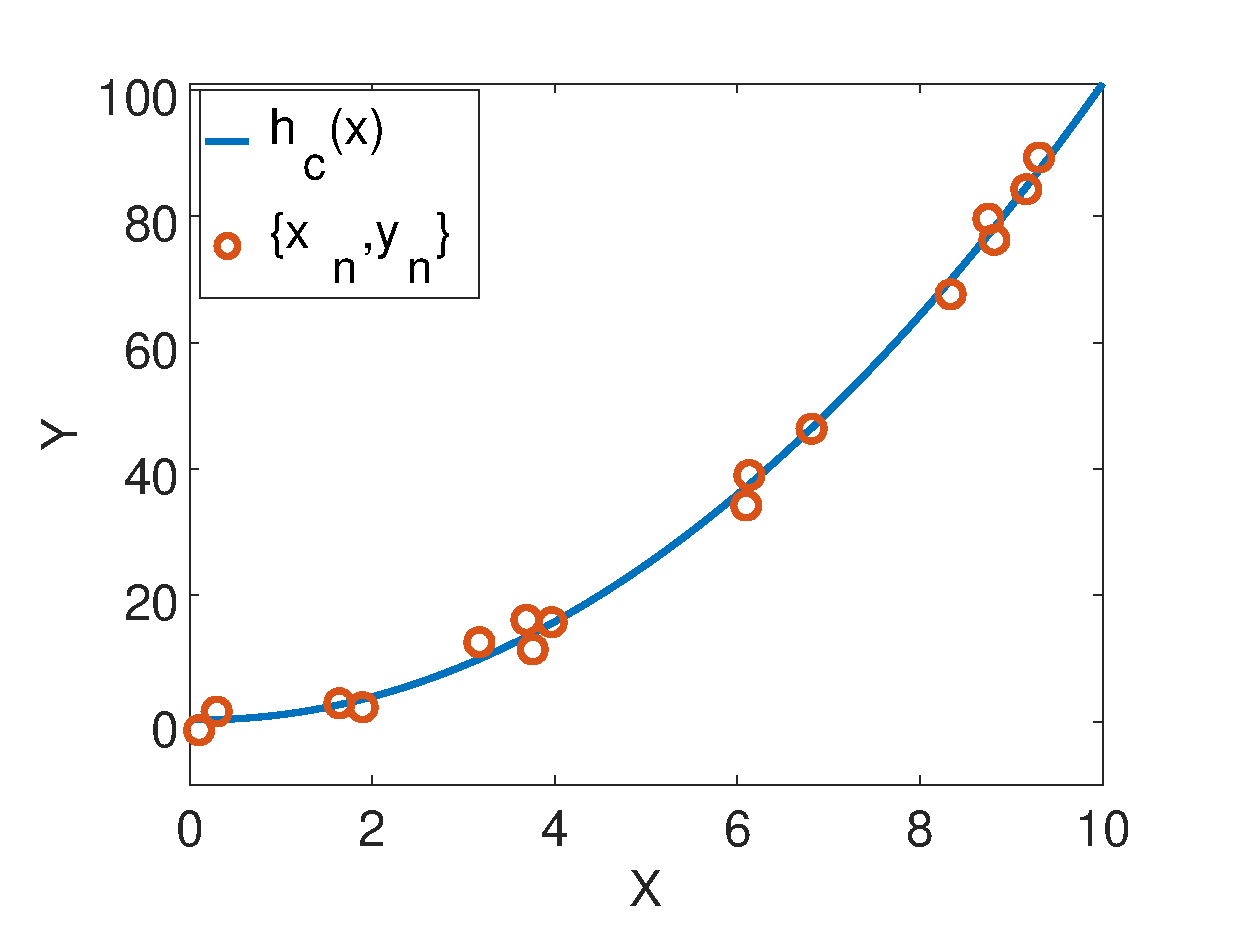
\includegraphics[width=0.49\textwidth]{chapters/mapeamento/mfiles/mapeamentor1r1/minimizando_hx.eps}
        \caption{Gráfico das amostras $\{x_n,y_n\}$ e da curva $x$ vs. $h_{\VECTOR{c}}(x)$.}
        \label{fig:theo:maphxr1r1:xnyn}
    \end{figure}

\end{SolutionT}




\newpage
%%%%%%%%%%%%%%%%%%%%%%%%%%%%%%%%%%%%%%%%%%%%%%%%%%%%%%%%%%%%%%%%%%%%%%%%%%%%%%%%%%%%%%%
%%%%%%%%%%%%%%%%%%%%%%%%%%%%%%%%%%%%%%%%%%%%%%%%%%%%%%%%%%%%%%%%%%%%%%%%%%%%%%%%%%%%%%%
%%%%%%%%%%%%%%%%%%%%%%%%%%%%%%%%%%%%%%%%%%%%%%%%%%%%%%%%%%%%%%%%%%%%%%%%%%%%%%%%%%%%%%%
\section{ Mapeamento com uma função $h_{\VECTOR{c}}(x):~\mathbb{R} \rightarrow \mathbb{R}$ }
\index{Problema inverso: Aplicado!Não linear}
\index{Regressão não linear!Simples!Função $h_{\VECTOR{c}}(x):~\mathbb{R} \rightarrow \mathbb{R}$}
\index{Mapeamento!Função $h_{\VECTOR{c}}(x):~\mathbb{R} \rightarrow \mathbb{R}$}


\begin{theorem}[Mapeamento usando uma função
$h_{\VECTOR{c}}(x)$:]
\label{theo:maphcxr1r1}
~\\
\begin{minipage}{0.4\textwidth}
\centering
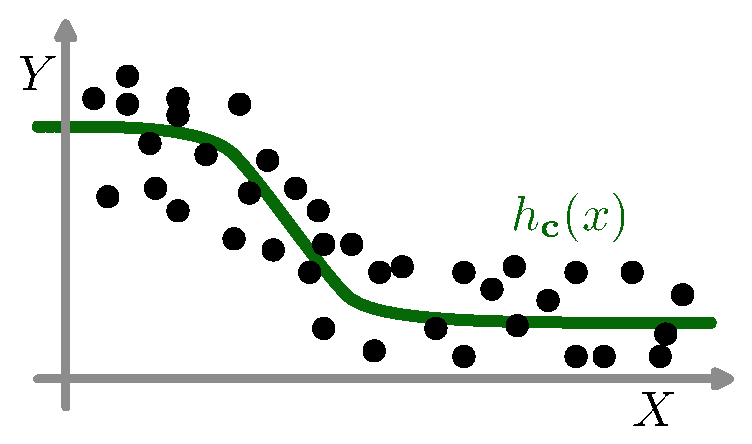
\includegraphics[width=0.95\linewidth]{chapters/mapeamento/mapeamento-hx-nonlinear.eps} 
\end{minipage}
\begin{minipage}{0.6\textwidth}
Dados,
os escalares $x \in \mathbb{R}$ e $y \in \mathbb{R}$, o vetor coluna $\VECTOR{c} \in \mathbb{R}^M$, e 
definida a Eq. (\ref{eq:maphcxr1r1:1}), 
\begin{equation}\label{eq:maphcxr1r1:1}
y=h_{\VECTOR{c}}(x)\equiv h(\VECTOR{c},x),
\end{equation}
onde $h_{\VECTOR{c}}:\mathbb{R} \rightarrow \mathbb{R}$, é uma função com dominio em $X$, contradominio em $Y$
e com coeficientes $c_m$ que formam o vetor $\VECTOR{c} \in \mathbb{R}^{M}$;
podemos afirmar que o vetor $\VECTOR{c}=\VECTOR{\hat{c}}$,
que minimiza o erro $e(\VECTOR{c})$,
\end{minipage}

\begin{equation}\label{eq:maphcxr1r1:2}
e(\VECTOR{c}) =  ||\VECTOR{h}(\VECTOR{c})-\VECTOR{y}||_{\MATRIX{W}}^2 + \alpha||\VECTOR{c}-\VECTOR{c}_{last}||_{\MATRIX{D}}^2,
\end{equation}
onde $\alpha \in \mathbb{R}$ é um multiplicador de Lagrange escolhido por nós,
\begin{equation}
\VECTOR{h}(\VECTOR{c})\equiv \VECTOR{h}_{\VECTOR{x}}(\VECTOR{c})=\begin{bmatrix}
h(\VECTOR{c},x_1)\\ 
h(\VECTOR{c},x_2)\\ 
%\vdots\\ 
%h(\VECTOR{c},x_n)\\ 
\vdots\\ 
h(\VECTOR{c},x_N)
\end{bmatrix},
~
%\VECTOR{x}=\begin{bmatrix}
%x_1\\ 
%x_2\\ 
%%\vdots\\ 
%%x_n\\ 
%\vdots\\ 
%x_N
%\end{bmatrix},
%~
\VECTOR{y}=\begin{bmatrix}
y_1\\ 
y_2\\ 
%\vdots\\ 
%y_n\\ 
\vdots\\ 
y_N
\end{bmatrix},
~
\MATRIX{W}=\funcdiag\left(\begin{bmatrix}
w_1\\ 
w_2\\ 
%\vdots\\ 
%w_n\\ 
\vdots\\ 
w_N
\end{bmatrix}\right),
~
\MATRIX{D}=\funcdiag\left(\begin{bmatrix}
d_1\\ 
d_2\\ 
%\vdots\\ 
%d_m\\ 
\vdots\\ 
d_M
\end{bmatrix}\right);
\end{equation}
pode ser achado\footnote{A demostração pode ser vista na Prova \ref{proof:theo:maphcxr1r1}.} 
usando de forma iterativa a Eq. (\ref{eq:maphcxr1r1:3})
\begin{equation}\label{eq:maphcxr1r1:3}
\VECTOR{c}_{i}=\VECTOR{c}_{i-1}-[\MATRIX{J}(\VECTOR{c}_{i-1})^{\transpose}\MATRIX{W}\MATRIX{J}(\VECTOR{c}_{i-1})+\alpha \MATRIX{D}]^{-1}\MATRIX{J}(\VECTOR{c}_{i-1})^{\transpose}\MATRIX{W}[\VECTOR{h}(\VECTOR{c}_{i-1})-\VECTOR{y}],
\end{equation}
onde a matriz $\MATRIX{J}(\VECTOR{c})$ 
$\equiv \frac{\partial \VECTOR{h}(\VECTOR{c})}{\partial \VECTOR{c}^{\transpose}}$ é a 
\hyperref[def:jacobian]{\textbf{matriz Jacobiana}}  de $\VECTOR{h}(\VECTOR{c})$,
\begin{equation}
\MATRIX{J}(\VECTOR{c})\equiv\MATRIX{J}_{\VECTOR{x}}(\VECTOR{c})=\begin{bmatrix}
\VECTOR{j}(\VECTOR{c},x_1)\\ 
\VECTOR{j}(\VECTOR{c},x_2)\\ 
%\vdots\\ 
%\VECTOR{j}(\VECTOR{c},x_n)\\ 
\vdots\\ 
\VECTOR{j}(\VECTOR{c},x_N)
\end{bmatrix},
\quad
\begin{array}{lll}
\VECTOR{j}(\VECTOR{c},x) & = & \frac{\partial h(\VECTOR{c},x)}{\partial \VECTOR{c}^{\transpose}} \\
                       ~ & ~ & ~\\
                       ~ & = & \left[\frac{\partial h(\VECTOR{c},x)}{\partial c_1}\quad \frac{\partial h(\VECTOR{c},x)}{\partial c_2}\quad ...\quad \frac{\partial h(\VECTOR{c},x)}{\partial c_{m}} \quad ... \quad \frac{\partial h(\VECTOR{c},x)}{\partial c_{M}} \right]
\end{array}
\end{equation}

\textbf{Considerações:}
\begin{itemize}
\item A busca iterativa da Eq. (\ref{eq:maphcxr1r1:3}) 
é declarada finalizada com sucesso 
quando iterações consecutivas do vetor $\VECTOR{c}_i$ convergem a valores próximos, onde declaramos $\VECTOR{\hat{c}}=\VECTOR{c}_i$.
\item O erro mínimo, $e(\VECTOR{\hat{c}}) \geq 0$, não necessariamente ter valor zero. 
\end{itemize}
\end{theorem}

%\begin{tcbattention}
%\begin{itemize}
%\item 
%\end{itemize}
%\end{tcbattention}

%%%%%%%%%%%%%%%%%%%%%%%%%%%%%%%%%%%%%%%%%%%%%%%%%%%%%%%%%%%%%%%%%%%%%%%%%%%%%%%%
\subsection{Exemplos de mapeamento usando uma função
$h(\VECTOR{c},x):~\mathbb{R} \rightarrow \mathbb{R}$}

\begin{example}\label{ex:theo:maphcxr1r1}
Conhecida as $N=18$ amostras $x_n$ e $y_n$, mostradas nas  Tabelas \ref{table:theo:maphcxr1r1:xn} e \ref{table:theo:maphcxr1r1:yn},
achar os parametros $c_m$ do vetor $\VECTOR{c}=[c_1\quad c_2\quad c_3]^{\transpose}$ da função $h(\VECTOR{c},x)$, 
\begin{equation}
h(\VECTOR{c},x)=c_1 e^{-\left(\frac{x}{c_2}\right)^{-4}}+c_3,
\end{equation}
que gere o menor erro 
$e(\VECTOR{c})=0.1 ||\VECTOR{c}-\VECTOR{c}_{last}||^2 + \sum_{n=1}^{N} ||h(\VECTOR{c},x_n)-y_n||^2 $.
\end{example}


\begin{table}[h!]
\centering
\begin{tabular}{|c|c|c|c|c|c|c|c|c|} 
 \hline
$n$   & 1 & 2 & 3 & 4 & 5 & 6 & 7 & 8\\ \hline
$x_n$ & 0.10461 & 0.29614 & 1.63968 & 1.89586 & 3.17301 & 3.68811 & 3.75758 & 3.96560 \\ \hline
 \hline
$n$   & 9 & 10 & 11 & 12 & 13 & 14 & 15 & 16\\  \hline
$x_n$ & 6.09526 & 6.12999 & 6.81288 & 8.33457 & 8.74851 & 8.81418 & 9.16269 & 9.30314 \\ \hline
\end{tabular}
\caption{Valores $x_n$.}
\label{table:theo:maphcxr1r1:xn}
\end{table}

\begin{table}[h!]
\centering
\begin{tabular}{|c|c|c|c|c|c|c|c|c|} 
 \hline
$n$   & 1 & 2 & 3 & 4 & 5 & 6 & 7 & 8\\ \hline
$y_n$ & 9.9005 & 10.1155 & 9.3351 & 8.7244 & 4.4788 & 3.0054 & 2.4827 & 2.3804  \\ \hline
 \hline
$n$   & 9 & 10 & 11 & 12 & 13 & 14 & 15 & 16\\  \hline
$y_n$ & 1.7806 & 2.1098 & 1.9972 & 1.8630 & 2.2316 & 1.8932 & 2.0231 & 2.2066 \\ \hline
\end{tabular}
\caption{Valores $y_n$.}
\label{table:theo:maphcxr1r1:yn}
\end{table}

\begin{SolutionT}[Relativa ao Exemplo \ref{ex:theo:maphcxr1r1}:]\label{sol:theo:maphcxr1r1}
Para obter  o vetor $\VECTOR{c}=\VECTOR{\hat{c}}$, da função $h(\VECTOR{c},x) = c_1~ e^{-\left(\frac{x}{c_2}\right)^{-4}}+c_3$,
%\begin{equation}
%h(\VECTOR{c},x)=c_1~ e^{-\left(\frac{x}{c_2}\right)^{-4}}+c_3,
%\end{equation} 
com o menor erro $e(\VECTOR{c})=0.1 ||\VECTOR{c}-\VECTOR{c}_{last}||^2 + \sum\limits_{n=1}^{N} ||h(\VECTOR{c},x_n)-y_n||^2 $,
podemos usar iterativamente a Eq. (\ref{eq:maphcxr1r1:3}), com 
\begin{equation}
\frac{\partial h(\VECTOR{c},x)}{\partial c_1} 
= e^{-\left(\frac{x}{c_2}\right)^{-4}},\qquad 
\frac{\partial h(\VECTOR{c},x)}{\partial c_2} 
= 4\frac{c_1}{c_2}\left(\frac{x}{c_2}\right)^{-4}e^{-\left(\frac{x}{c_2}\right)^{-4}}, \qquad 
\frac{\partial h(\VECTOR{c},x)}{\partial c_3} 
=1
\end{equation} 
iniciando desde um vetor $\VECTOR{c}_{0}=[1\quad 1\quad 1]^{\transpose}$ escolhido arbitrariamente.
Obtendo assim a Tabela \ref{table:theo:maphcxr1r1:ei}, que conclui em
$\VECTOR{\hat{c}}=\VECTOR{c}_{5}=[7.9767\quad 3.0212\quad 2.0039]^{\transpose}$,
com  um erro $e(\VECTOR{c}_{5})=0.31848$.


\begin{table}[h!]
\centering
\begin{tabular}{|c|c|c|c|c|c|c|} 
 \hline
$i$   & 0 & 1 & 2 & 3 & 4 & 5 \\ \hline
\hline
$c_1$ & 1.0000 & 6.4006 & 7.5254 & 7.9571 & 7.9759 & 7.9767 \\ \hline
$c_2$ & 1.0000 & 2.3743 & 3.0158 & 3.0210 & 3.0212 & 3.0212 \\ \hline
$c_3$ & 1.0000 & 3.3416 & 2.2483 & 2.0111 & 2.0042 & 2.0039 \\ \hline
\hline
$e(\VECTOR{c}_{i})$ & 286.15891 & 19.10286 & 1.05792 & 0.31951 & 0.31848 & 0.31848  \\ \hline
\end{tabular}
\caption{Valores $e(\VECTOR{c}_{i})$ e vetores $\VECTOR{c}_{i}$.}
\label{table:theo:maphcxr1r1:ei}
\end{table}

    \begin{figure}[!h]
        \centering
        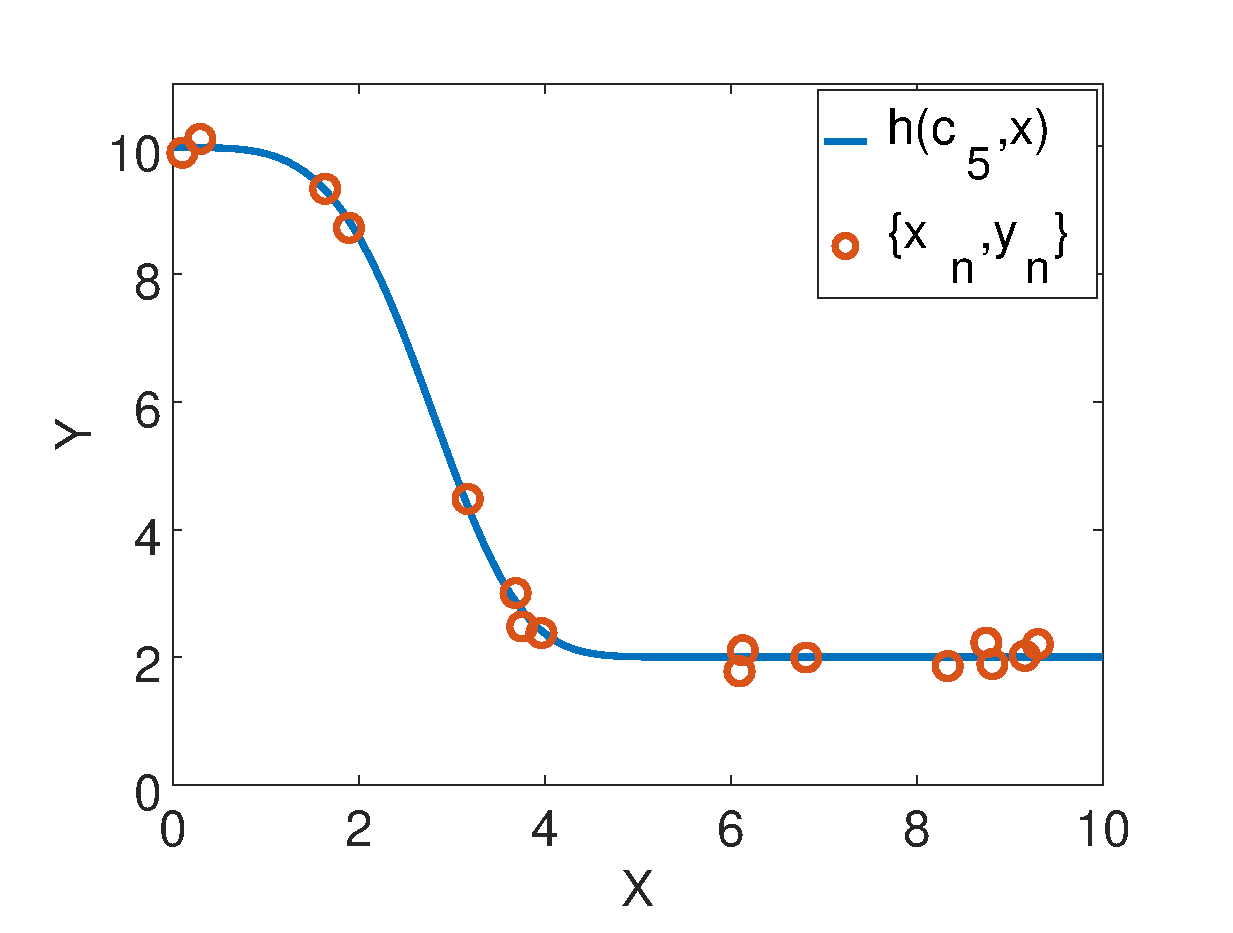
\includegraphics[width=0.49\textwidth]{chapters/mapeamento/mfiles/mapeamentor1r1-nonlinear/minimizando_hx.eps}
        \caption{Gráfico das amostras $\{x_n,y_n\}$ e da curva $x$ vs. $h(\VECTOR{c}_5,x)$.}
        \label{fig:theo:maphcxr1r1:xnyn}
    \end{figure}

\end{SolutionT}




\newpage
%%%%%%%%%%%%%%%%%%%%%%%%%%%%%%%%%%%%%%%%%%%%%%%%%%%%%%%%%%%%%%%%%%%%%%%%%%%%%%%%%%%%%%%
%%%%%%%%%%%%%%%%%%%%%%%%%%%%%%%%%%%%%%%%%%%%%%%%%%%%%%%%%%%%%%%%%%%%%%%%%%%%%%%%%%%%%%%
%%%%%%%%%%%%%%%%%%%%%%%%%%%%%%%%%%%%%%%%%%%%%%%%%%%%%%%%%%%%%%%%%%%%%%%%%%%%%%%%%%%%%%%
\section{Regressão polinomial múltipla com $h_{\VECTOR{c}}(x,y):\mathbb{R}^2 \rightarrow \mathbb{R}$}
\label{sec:theo:maphxr2r1}

\index{Problema inverso: Aplicado!Linear}
\index{Regressão não linear!Múltipla!Polinômio $h_{\VECTOR{c}}(x,y):~\mathbb{R}^2 \rightarrow \mathbb{R}$}
\index{Regressão!Polinômio $h_{\VECTOR{c}}(x,y):~\mathbb{R}^2 \rightarrow \mathbb{R}$}

\begin{theorem}[Regressão usando um polinômio 
$h_{\VECTOR{c}}(x,y)$ de grau $M$:]
\label{theo:maphxr2r1}
~\\
\begin{minipage}{0.4\textwidth}
\centering
\includegraphics[width=0.95\linewidth]{chapters/mapeamento/mapeamento-hx2.eps} 
\end{minipage}
\begin{minipage}{0.6\textwidth}
Dados
os escalares $x \in \mathbb{R}$, $y \in \mathbb{R}$, $z \in \mathbb{R}$ e $c_m \in \mathbb{R}$,
uma função polinomial $h_{\VECTOR{c}}:\mathbb{R}^2 \rightarrow \mathbb{R}$, de grau $M$, e 
definida a Eq. (\ref{eq:maphxr2r1:1}),
\begin{equation}\label{eq:maphxr2r1:1}
z= h_{\VECTOR{c}}(x,y) = \sum \limits_{m=0}^{M} \sum \limits_{l=0}^{m}c_{\left\{ \frac{m(m+1)}{2}+l+1\right\}}~x^{m-l}y^{l}; 
\end{equation}
podemos afirmar que o vetor coluna $\VECTOR{c}=\VECTOR{\hat{c}} \in \mathbb{R}^{\frac{(M+1)(M+2)}{2}}$,
que minimiza o erro $e(\VECTOR{c})$,
\end{minipage}
\begin{equation}\label{eq:maphxr2r1:2}
%e(\VECTOR{c}) = ||h(\VECTOR{x})-\VECTOR{y}||_{\MATRIX{W}}^2 \equiv \sum_{n=1}^{N} w_n||h(x_n)-y_n||^2,
e(\VECTOR{c}) \equiv e(\VECTOR{c},\VECTOR{x},\VECTOR{y},\VECTOR{z},\MATRIX{w})=  \sum_{n=1}^{N} w_n||h_{\VECTOR{c}}(x_n,y_n)-z_n||^2,
\end{equation}
proveniente de avaliar $N$ amostras $\{x_n,y_n\}$ e $z_n$ que não cumprem necessariamente a Eq. (\ref{eq:maphxr2r1:1}), 
representadas pelos vetores 
$\VECTOR{x}=[x_1~ x_2~ ...~ x_n~ ...~ x_N]^{\transpose}$,
$\VECTOR{y}=[y_1~ y_2~ ...~ y_n~ ...~ y_N]^{\transpose}$ e 
$\VECTOR{z}=[z_1~ z_2~ ...~ z_n~ ...~ z_N]^{\transpose}$,
ponderadas com os pesos $w_n \in \mathbb{R}_+$, 
representados pela matriz diagonal $\MATRIX{W}=\funcdiag([w_1~ w_2~ ...~ w_n~ ...~ w_N]^{\transpose})$;
pode ser achado\footnote{A demonstração pode ser vista na Prova \ref{proof:theo:maphxr2r1}.} usando:
\begin{equation}\label{eq:maphxr2r1:3}
\VECTOR{\hat{c}}=[\MATRIX{A}^{\transpose}\MATRIX{W}\MATRIX{A}]^{-1}\MATRIX{A}^{\transpose}\MATRIX{W}\VECTOR{z},
\end{equation}
sendo a matriz $\MATRIX{A}$ definida como,
\begin{equation}\label{eq:maphxr2r1:4}
\MATRIX{A}\equiv\MATRIX{A}(\VECTOR{x},\VECTOR{y})=\begin{bmatrix}
\VECTOR{a}(x_1,y_1)\\
\VECTOR{a}(x_2,y_2)\\
\vdots\\
\VECTOR{a}(x_N,y_N)\\
\end{bmatrix}, \qquad
\begin{matrix}
\VECTOR{a}(x,y)= &
\begin{bmatrix}
\VECTOR{s}_{0}(x,y) & \VECTOR{s}_{1}(x,y) &  \dots  & \VECTOR{s}_{M}(x,y)
\end{bmatrix},\\
~&~\\
\VECTOR{s}_{m}(x,y)=&
\begin{bmatrix}
x^m  & x^{m-1} y  & x^{m-2} y^2    & \dots  & x y^{m-1} &  y^m 
\end{bmatrix}.
\end{matrix}
\end{equation}
\end{theorem}


\begin{tcbattention}
\begin{itemize}
%\begin{comment}
\item Para que o vetor $\VECTOR{c}$
que minimiza $e(\VECTOR{c})$ tenha resposta única,
é necessário (porém não suficiente) que  $N\geq \frac{(M+1)(M+2)}{2}$.
%\end{comment}
\item De forma exata, podemos afirmar que para que $\VECTOR{c}$ tenha resposta única,
deve existir a inversa da matriz $\MATRIX{A}^{\transpose}\MATRIX{W}\MATRIX{A}$.
\end{itemize}
\end{tcbattention}

\begin{corollary}[Função $\getminparam$ para o cálculo do vetor 
$\VECTOR{c}$ do polinômio $h_{\VECTOR{c}}(x,y)$ de grau $M$:]\label{coro:maphxr2r1}
Conhecidas as Eq. (\ref{eq:maphxr2r1:1}) e (\ref{eq:maphxr2r1:4}), 
podemos definir a seguinte equivalência:
\begin{equation}
z = h_{\VECTOR{c}}(x,y)\qquad \leftrightarrow  \qquad z = \VECTOR{a}(x,y)\VECTOR{c}.
\end{equation}
Para obter o vetor $\VECTOR{c}=\VECTOR{\hat{c}}$ que minimiza a função $e(\VECTOR{c})$
da Eq. (\ref{eq:maphxr2r1:2}), 
são usadas as Equações (\ref{eq:maphxr2r1:3}) e (\ref{eq:maphxr2r1:4}),
os dados $\VECTOR{x}$, $\VECTOR{y}$, $\VECTOR{z}$ e $\MATRIX{w}$, e definida
a função $\getminparam$ como:
\begin{equation}
\begin{array}{lllll}
\VECTOR{\hat{c}} & = & 
\getminparam (\VECTOR{x},\VECTOR{y},\VECTOR{z},\MATRIX{W}) & = & 
[\MATRIX{A}(\VECTOR{x},\VECTOR{y})^{\transpose}\MATRIX{W}\MATRIX{A}(\VECTOR{x},\VECTOR{y})]^{-1}\MATRIX{A}(\VECTOR{x},\VECTOR{y})^{\transpose}\MATRIX{W}\VECTOR{z}.
\end{array}
\end{equation}
\end{corollary}

%%%%%%%%%%%%%%%%%%%%%%%%%%%%%%%%%%%%%%%%%%%%%%%%%%%%%%%%%%%%%%%%%%%%%%%%%%%%%%%%
\subsection{Exemplos de regressão com um polinômio
$h_{\VECTOR{c}}(x,y):~\mathbb{R}^2 \rightarrow \mathbb{R}$ de grau $M$ }

\begin{example}\label{ex:theo:maphxr2r1}
Conhecida as $N=16$ amostras $\{x_n,y_n\}$ e $z_n$, 
mostradas nas  Tabelas \ref{table:theo:maphxr2r1:xnyn} e \ref{table:theo:maphxr2r1:zn},
achar o polinômio $h_{\VECTOR{c}}(x,y)$ de grau $M=2$,
\begin{equation}
h_{\VECTOR{c}}(x,y) = c_{1}+c_{2}~x + c_{3}~y +c_{4}~x^2 +c_{5}~xy + c_{6}~y^2;
\end{equation} 
que gere o menor erro $e(\VECTOR{c}) =  \sum_{n=1}^{N} ||h_{\VECTOR{c}}(x_n,y_n)-z_n||^2$.
\end{example}


\begin{table}[h!]
\centering
\begin{tabular}{|c|c|c|c|c|c|c|c|c|} 
 \hline
$n$   & 1 & 2 & 3 & 4 & 5 & 6 & 7 & 8\\ \hline
$x_n$ & 5.24910 & 5.28850 & 5.58188 & 2.25455 & 0.17769 & 3.65716 & 5.00074 & 2.37936 \\ \hline
$y_n$ & 5.80108 & 2.29459 & 2.94123 & 4.97383 & 4.84170 & 3.20595 & 2.36837 & 1.46028 \\ \hline
 \hline
$n$   & 9 & 10 & 11 & 12 & 13 & 14 & 15 & 16\\  \hline
$x_n$ & 1.13752 & 5.49762 & 4.08773 & 1.90381 & 0.06277 & 0.98381 & 3.67799 & 2.21287 \\ \hline
$y_n$ & 0.01718 & 3.69885 & 5.13457 & 5.56777 & 4.26294 & 3.95342 & 5.68502 & 1.08792 \\ \hline
\end{tabular}
\caption{Valores $\{x_n,y_n\}$.}
\label{table:theo:maphxr2r1:xnyn}
\end{table}



\begin{table}[h!]
\centering
\begin{tabular}{|c|c|c|c|c|c|c|c|c|} 
 \hline
$n$   & 1 & 2 & 3 & 4 & 5 & 6 & 7 & 8\\ \hline
$z_n$ & 103.6067 & 54.0677 & 65.7671 & 49.1678 & 30.5434 & 43.4313 & 50.6294 & 16.1106  \\ \hline
 \hline
$n$   & 9 & 10 & 11 & 12 & 13 & 14 & 15 & 16\\  \hline
$z_n$ & 3.2491 & 74.5464 & 74.2815 & 53.5591 & 24.0016 & 26.3172 & 77.1427 & 12.9952 \\ \hline
\end{tabular}
\caption{Valores $z_n$.}
\label{table:theo:maphxr2r1:zn}
\end{table}

     

\begin{SolutionT}[Relativa ao Exemplo \ref{ex:theo:maphxr2r1}:]\label{sol:theo:maphxr2r1}
Para obter o polinômio $h_{\VECTOR{c}}(x,y)$ de grau $M=2$, 
que gere o menor erro $e(\VECTOR{c}) =  \sum_{n=1}^{N} ||h_{\VECTOR{c}}(x_n,y_n)-z_n||^2$,
usamos a Eq. (\ref{eq:maphxr2r1:1}); o vetor $\VECTOR{c}$ é calculado mediante a Eq. (\ref{eq:maphxr2r1:3}),
na qual obtemos que $\VECTOR{c}=[0.96676$ $0.91808$ $1.17077$ $1.00515$ $1.00873$ $0.9698]^{\transpose}$, de modo que
\begin{equation}
h_{\VECTOR{c}}(x,y) =   0.96676 +0.91808 x +1.17077 y +1.00515 x^2 +1.00873 xy +0.96980 y^2.
\end{equation}
    \begin{figure}[!h]
        \centering
        \includegraphics[width=0.49\textwidth]{chapters/mapeamento/mfiles/mapeamentor2r1/minimizando_hx.eps}
        \caption{Gráfico das amostras $\{x_n,y_n,z_n\}$ e da superfície $z=h_{\VECTOR{c}}(x,y)$.}
        \label{fig:theo:maphxr2r1:xnyn}
    \end{figure}

\end{SolutionT}




\newpage
%%%%%%%%%%%%%%%%%%%%%%%%%%%%%%%%%%%%%%%%%%%%%%%%%%%%%%%%%%%%%%%%%%%%%%%%%%%%%%%%%%%%%%%
%%%%%%%%%%%%%%%%%%%%%%%%%%%%%%%%%%%%%%%%%%%%%%%%%%%%%%%%%%%%%%%%%%%%%%%%%%%%%%%%%%%%%%%
%%%%%%%%%%%%%%%%%%%%%%%%%%%%%%%%%%%%%%%%%%%%%%%%%%%%%%%%%%%%%%%%%%%%%%%%%%%%%%%%%%%%%%%
\section{Regressão não linear múltipla com $h_{\VECTOR{c}}(\VECTOR{x}):~\mathbb{R}^N \rightarrow \mathbb{R}$}
\label{sec:theo:maphcxrnr1}

\index{Problema inverso: Aplicado!Não linear}
\index{Regressão não linear!Múltipla!Função $h_{\VECTOR{c}}(\VECTOR{x}):~\mathbb{R}^N \rightarrow \mathbb{R}$}
\index{Regressão!Função $h_{\VECTOR{c}}(\VECTOR{x}):~\mathbb{R}^N \rightarrow \mathbb{R}$}


\begin{theorem}[Regressão usando uma função não linear
$h_{\VECTOR{c}}(\VECTOR{x})$:]
\label{theo:maphcxrnr1}
~\\
\begin{minipage}{0.4\textwidth}
\centering
\includegraphics[width=0.95\linewidth]{chapters/mapeamento/mapeamento-hxn-nonlinear.eps} 
\end{minipage}
\begin{minipage}{0.6\textwidth}
Dados 
um conjunto de $L$ amostras
do escalar $z_l \in \mathbb{R}$ e do vetor $\VECTOR{x}_l \in \mathbb{R}^N$, $1\leq l\leq L$, e 
definida a Eq. (\ref{eq:maphcxrnr1:1}), 
\begin{equation}\label{eq:maphcxrnr1:1}
z=h_{\VECTOR{c}}(\VECTOR{x})\equiv h(\VECTOR{c},\VECTOR{x}),
\end{equation}
na qual $h_{\VECTOR{c}}:\mathbb{R}^N \rightarrow \mathbb{R}$ 
é uma função com domínio em  $\VECTOR{x} \in \mathbb{R}^N$, contradomínio em $z\in \mathbb{R}$
e com coeficientes $c_m$ que formam o vetor $\VECTOR{c}\in \mathbb{R}^{M}$;
podemos afirmar que o vetor $\VECTOR{c}=\VECTOR{\hat{c}}$
que minimiza o erro $e(\VECTOR{c})$,
\end{minipage}

\begin{equation}\label{eq:maphcxrnr1:2}
e(\VECTOR{c}) =  ||\VECTOR{h}(\VECTOR{c})-\VECTOR{z}||_{\MATRIX{W}}^2 + \alpha||\VECTOR{c}-\VECTOR{c}_{last}||_{\MATRIX{D}}^2,
\end{equation}
em que $w_l \in \mathbb{R}_+$, $d_l \in \mathbb{R}_+$, e $\alpha \in \mathbb{R}_+$ são valores escolhidos por nós,
\begin{equation}
\VECTOR{h}(\VECTOR{c})=\begin{bmatrix}
h(\VECTOR{c},\VECTOR{x}_1)\\ 
h(\VECTOR{c},\VECTOR{x}_2)\\ 
%\vdots\\ 
%h(\VECTOR{c},\VECTOR{x}_l)\\ 
\vdots\\ 
h(\VECTOR{c},\VECTOR{x}_L)
\end{bmatrix},
~
%\MATRIX{P}=\begin{bmatrix}
%\VECTOR{x}_1^{\transpose}\\ 
%\VECTOR{x}_2^{\transpose}\\ 
%%\vdots\\ 
%%\VECTOR{x}_l^{\transpose}\\ 
%\vdots\\ 
%\VECTOR{x}_L^{\transpose}
%\end{bmatrix},
%~
\VECTOR{z}=\begin{bmatrix}
z_1\\ 
z_2\\ 
%\vdots\\ 
%z_l\\ 
\vdots\\ 
z_L
\end{bmatrix},
~
\MATRIX{W}=\funcdiag\left(\begin{bmatrix}
w_1\\ 
w_2\\ 
%\vdots\\ 
%w_l\\ 
\vdots\\ 
w_L
\end{bmatrix}\right),
~
\MATRIX{D}=\funcdiag\left(\begin{bmatrix}
d_1\\ 
d_2\\ 
%\vdots\\ 
%d_m\\ 
\vdots\\ 
d_L
\end{bmatrix}\right);
\end{equation}
pode ser achado\footnote{A demonstração pode ser vista na Prova \ref{proof:theo:maphcxrnr1}.} 
usando de forma iterativa a Eq. (\ref{eq:maphcxrnr1:3})
\begin{equation}\label{eq:maphcxrnr1:3}
\VECTOR{c}_{i}=\VECTOR{c}_{i-1}-[\MATRIX{J}(\VECTOR{c}_{i-1})^{\transpose}\MATRIX{W}\MATRIX{J}(\VECTOR{c}_{i-1})+\alpha \MATRIX{D}]^{-1}\MATRIX{J}(\VECTOR{c}_{i-1})^{\transpose}\MATRIX{W}[\VECTOR{h}(\VECTOR{c}_{i-1})-\VECTOR{z}],
\end{equation}
na qual a matriz $\MATRIX{J}(\VECTOR{c})$ 
$\equiv \frac{\partial \VECTOR{h}(\VECTOR{c})}{\partial \VECTOR{c}^{\transpose}}$ é a 
\hyperref[def:jacobian]{\textbf{matriz Jacobiana}}  de $\VECTOR{h}(\VECTOR{c})$,
\begin{equation}
\MATRIX{J}(\VECTOR{c})=\begin{bmatrix}
\VECTOR{j}(\VECTOR{c},\VECTOR{x}_1)\\ 
\VECTOR{j}(\VECTOR{c},\VECTOR{x}_2)\\ 
%\vdots\\ 
%\VECTOR{j}(\VECTOR{c},\VECTOR{x}_l)\\ 
\vdots\\ 
\VECTOR{j}(\VECTOR{c},\VECTOR{x}_L)
\end{bmatrix},
\quad
\begin{array}{lll}
\VECTOR{j}(\VECTOR{c},\VECTOR{x}) & = & \frac{\partial h(\VECTOR{c},\VECTOR{x})}{\partial \VECTOR{c}^{\transpose}} \\
                       ~ & ~ & ~\\
                       ~ & = & \left[\frac{\partial h(\VECTOR{c},\VECTOR{x})}{\partial c_1}\quad \frac{\partial h(\VECTOR{c},\VECTOR{x})}{\partial c_2}\quad ...\quad \frac{\partial h(\VECTOR{c},\VECTOR{x})}{\partial c_{m}} \quad ... \quad \frac{\partial h(\VECTOR{c},\VECTOR{x})}{\partial c_{M}} \right].
\end{array}
\end{equation}

\textbf{Considerações:}
\begin{itemize}
\item A busca iterativa da Eq. (\ref{eq:maphcxrnr1:3}) 
é declarada finalizada com sucesso 
quando iterações consecutivas do vetor $\VECTOR{c}_i$ convergem a valores próximos, 
momento no qual declaramos que $\VECTOR{\hat{c}}=\VECTOR{c}_i$.
\item O erro mínimo $e(\VECTOR{\hat{c}}) \geq 0$, não necessariamente obtem o valor zero. 
\end{itemize}
\end{theorem}

%\begin{tcbattention}
%\begin{itemize}
%\item 
%\end{itemize}
%\end{tcbattention}

%%%%%%%%%%%%%%%%%%%%%%%%%%%%%%%%%%%%%%%%%%%%%%%%%%%%%%%%%%%%%%%%%%%%%%%%%%%%%%%%
\subsection{Exemplos de regressão usando uma função
$h_{\VECTOR{c}}(\VECTOR{x}):~\mathbb{R}^N \rightarrow \mathbb{R}$}

\begin{example}\label{ex:theo:maphcxrnr1}
Conhecida as $L=16$ amostras $\VECTOR{x}_l$ e $z_l$, mostradas nas  
Tabelas \ref{table:theo:maphcxrnr1:xn} e \ref{table:theo:maphcxrnr1:zn},
achar os parametros $c_m$ do vetor $\VECTOR{c}=[c_1\quad c_2\quad c_3]^{\transpose}$ da função $h(\VECTOR{c},\VECTOR{x})$, 
\vspace{-6pt}
\begin{equation}
h(\VECTOR{c},\VECTOR{x})=c_1 e^{-\left(\frac{x_1}{c_2}\right)^{-4}-\left(\frac{x_2}{c_2}\right)^{-4}}+c_3,
\end{equation}
que gere o menor erro 
$e(\VECTOR{c})=\sum_{l=1}^{L} ||h(\VECTOR{c},\VECTOR{x}_l)-z_l||^2 + 0.1 ||\VECTOR{c}-\VECTOR{c}_{last}||^2$.
\end{example}


\begin{table}[h!]
\centering
\begin{tabular}{|c|c|c|c|c|c|c|c|c|} 
 \hline
$l$   & 1 & 2 & 3 & 4 & 5 & 6 & 7 & 8\\ \hline
$\VECTOR{x}_l$ & 5.24910 & 5.28851 & 5.58188 & 2.25455 & 0.17769 & 3.65716 & 5.00074 & 2.37936 \\ 
             ~ & 5.80108 & 2.29459 & 2.94123 & 4.97383 & 4.84170 & 3.20595 & 2.36837 & 1.46028 \\ \hline
 \hline
$l$   & 9 & 10 & 11 & 12 & 13 & 14 & 15 & 16\\  \hline
$\VECTOR{x}_l$ & 1.13752 & 5.49762 & 4.08773 & 1.90381 & 0.06277 & 0.98381 & 3.67799 & 2.21287 \\
             ~ & 0.01718 & 3.69885 & 5.13457 & 5.56777 & 4.26294 & 3.95342 & 5.68502 & 1.08792 \\ \hline
\end{tabular}
\caption{Valores $\VECTOR{x}_l$.}
\label{table:theo:maphcxrnr1:xn}
\end{table}

\begin{table}[h!]
\centering
\begin{tabular}{|c|c|c|c|c|c|c|c|c|} 
 \hline
$l$   & 1 & 2 & 3 & 4 & 5 & 6 & 7 & 8\\ \hline
$y_l$ & 1.9005 & 2.1166 & 2.0181 & 1.9069 & 2.1991 & 2.4291 & 1.8024 & 7.0944  \\ \hline
 \hline
$l$   & 9 & 10 & 11 & 12 & 13 & 14 & 15 & 16\\  \hline
$y_l$ & 9.6170 & 2.1098 & 1.9972 & 1.8631 & 2.3673 & 2.2807 & 2.0231 & 8.0547 \\ \hline
\end{tabular}
\caption{Valores $y_l$.}
\label{table:theo:maphcxrnr1:zn}
\end{table}


\begin{SolutionT}[Relativa ao Exemplo \ref{ex:theo:maphcxrnr1}:]\label{sol:theo:maphcxrnr1}
Para obter  o vetor $\VECTOR{c}=\VECTOR{\hat{c}}$
que provoque o menor erro $e(\VECTOR{c})$,
podemos usar iterativamente a Eq. (\ref{eq:maphcxrnr1:3}), com 
\begin{equation}
\frac{\partial h(\VECTOR{c},\VECTOR{x})}{\partial c_1} 
= e^{-\left(\frac{x_1}{c_2}\right)^{-4}-\left(\frac{x_2}{c_2}\right)^{-4}},\qquad 
\frac{\partial h(\VECTOR{c},\VECTOR{x})}{\partial c_2} 
= 4\frac{c_1}{c_2}\left(\left(\frac{x_1}{c_2}\right)^{-4}+\left(\frac{x_2}{c_2}\right)^{-4}\right)e^{-\left(\frac{x_1}{c_2}\right)^{-4}-\left(\frac{x_2}{c_2}\right)^{-4}}, 
\end{equation} 
$\frac{\partial h(\VECTOR{c},\VECTOR{x})}{\partial c_3} =1$,
iniciando em $\VECTOR{c}_{0}=[3\quad 2\quad 1]^{\transpose}$ escolhido arbitrariamente.
Obtendo assim a Tabela \ref{table:theo:maphcxrnr1:ei}, que conclui em
$\VECTOR{\hat{c}}=\VECTOR{c}_{5}=[7.8170\quad 3.0761\quad 1.9981]^{\transpose}$,
com  um erro $e(\VECTOR{c}_{5})=0.27067$.
\begin{table}[h!]
\centering
\begin{tabular}{|c|c|c|c|c|c|c|} 
 \hline
$i$   & 0 & 1 & 2 & 3 & 4 & 5 \\ \hline
\hline
$c_1$ & 3.0000 & 6.2450 & 5.2762 & 7.5557 & 7.7751 & 7.8170 \\ \hline
$c_2$ & 2.0000 & 4.6303 & 2.9364 & 3.1952 & 3.0813 & 3.0761 \\ \hline
$c_3$ & 1.0000 & 2.1159 & 3.3712 & 2.0283 & 2.0026 & 1.9981 \\ \hline
\hline
$e(\VECTOR{c}_{i})$ & 125.55885 & 45.42202 & 25.33905 & 0.47703 & 0.27315 & 0.27067  \\ \hline
\end{tabular}
\caption{Valores $e(\VECTOR{c}_{i})$ e vetores $\VECTOR{c}_{i}$.}
\label{table:theo:maphcxrnr1:ei}
\end{table}

    \begin{figure}[!h]
        \centering
        \includegraphics[width=0.48\textwidth]{chapters/mapeamento/mfiles/mapeamentornr1-nonlinear/minimizando_hx.eps}
        \caption{Gráfico das amostras $\{\VECTOR{x}_l,z_l\}$ e da superfície $z=h(\VECTOR{c}_5,\VECTOR{x})$.}
        \label{fig:theo:maphcxrnr1:xnyn}
    \end{figure}

\end{SolutionT}




\newpage
%%%%%%%%%%%%%%%%%%%%%%%%%%%%%%%%%%%%%%%%%%%%%%%%%%%%%%%%%%%%%%%%%%%%%%%%%%%%%%%%%%%%%%%
%%%%%%%%%%%%%%%%%%%%%%%%%%%%%%%%%%%%%%%%%%%%%%%%%%%%%%%%%%%%%%%%%%%%%%%%%%%%%%%%%%%%%%%
%%%%%%%%%%%%%%%%%%%%%%%%%%%%%%%%%%%%%%%%%%%%%%%%%%%%%%%%%%%%%%%%%%%%%%%%%%%%%%%%%%%%%%%
\section{Regressão polinomial múltipla com $\VECTOR{h}(x,y):~\mathbb{R}^2 \rightarrow \mathbb{R}^2$}
\label{sec:theo:maphxr2r2}

\index{Problema inverso: Aplicado!Linear}
\index{Regressão não linear!Múltipla!Polinômio $\VECTOR{h}(x,y):~\mathbb{R}^2 \rightarrow \mathbb{R}^2$}
\index{Regressão!Polinômio $\VECTOR{h}(x,y):~\mathbb{R}^2 \rightarrow \mathbb{R}^2$}

\begin{theorem}[Regressão usando um polinômio 
$\VECTOR{f}(x,y):$ $\mathbb{R}^2 \rightarrow \mathbb{R}^2$, de grau $M$:]
\label{theo:maphxr2r2}
~\\
\begin{minipage}{0.45\textwidth}
\centering
\includegraphics[width=0.85\linewidth]{chapters/mapeamento/mapeamento.eps} 
\end{minipage}
\begin{minipage}{0.55\textwidth}
Dados
os escalares 
$x \in \mathbb{R}$, 
$y \in \mathbb{R}$, 
$u \in \mathbb{R}$ e 
$v \in \mathbb{R}$,
os vetores $\VECTOR{c} \in \mathbb{R}^{\frac{(M+1)(M+2)}{2}}$ e
$\VECTOR{d} \in \mathbb{R}^{\frac{(M+1)(M+2)}{2}}$,
com elementos $c_k$ e $d_k$,
uma função polinomial $\VECTOR{h}:\mathbb{R}^2 \rightarrow \mathbb{R}^2$, de grau $M$, e 
definida a Eq. (\ref{eq:maphxr2r2:1}),
\begin{equation}\label{eq:maphxr2r2:1}
\begin{bmatrix}
u\\
v
\end{bmatrix} =
\VECTOR{h}(x,y) \equiv 
\begin{bmatrix}
h_{\VECTOR{c}}(x,y)\\
h_{\VECTOR{d}}(x,y)
\end{bmatrix}
\end{equation}
\end{minipage}
\noindent
\begin{equation}\label{eq:maphxr2r2:1a}
h_{\VECTOR{c}}(x,y) = \sum \limits_{m=0}^{M} \sum \limits_{l=0}^{m}c_{\left\{ \frac{m(m+1)}{2}+l+1\right\}}~x^{m-l}y^{l}, 
~~~
h_{\VECTOR{d}}(x,y) = \sum \limits_{m=0}^{M} \sum \limits_{l=0}^{m}d_{\left\{ \frac{m(m+1)}{2}+l+1\right\}}~x^{m-l}y^{l}; 
\end{equation}
%\begin{equation}\label{eq:maphxr2r2:1b}
%\end{equation}
podemos afirmar que os vetores coluna $\VECTOR{c}=\VECTOR{\hat{c}}$ e
$\VECTOR{d}=\VECTOR{\hat{d}}$,
que minimizam os erros $e_{\VECTOR{c}}(\VECTOR{c})$ e $e_{\VECTOR{d}}(\VECTOR{d})$,
respetivamente,
\begin{equation}\label{eq:maphxr2r2:2}
%e(\VECTOR{c}) = ||h(\VECTOR{x})-\VECTOR{y}||_{\MATRIX{W}}^2 \equiv \sum_{n=1}^{N} w_n||h(x_n)-y_n||^2,
e_{\VECTOR{c}}(\VECTOR{c}) =  \sum_{n=1}^{N} w_n||h_{\VECTOR{c}}(x_n,y_n)-u_n||^2,\qquad 
e_{\VECTOR{d}}(\VECTOR{d}) =  \sum_{n=1}^{N} w_n||h_{\VECTOR{d}}(x_n,y_n)-v_n||^2,
\end{equation}
proveniente de avaliar $N$ amostras $\{x_n,y_n\}$ e $\{u_n,v_n\}$ 
que não cumprem necessariamente a Eq. (\ref{eq:maphxr2r2:1}), 
representadas pelos vetores 
$\VECTOR{x}=[x_1~ ...~ x_n~ ...~ x_N]^{\transpose}$,
$\VECTOR{y}=[y_1~ ...~ y_n~ ...~ y_N]^{\transpose}$, 
$\VECTOR{u}=[u_1~ ...~ u_n~ ...~ u_N]^{\transpose}$, e
$\VECTOR{v}=[v_1~ ...~ v_n~ ...~ v_N]^{\transpose}$,
ponderadas com os pesos $w_n \in \mathbb{R}_+$, 
representados pela matriz diagonal $\MATRIX{W}=\funcdiag([w_1~ w_2~ ...~ w_n~ ...~ w_N]^{\transpose})$;
podem ser achados\footnote{A demonstração pode ser vista na Prova \ref{proof:theo:maphxr2r2}.} usando:
\begin{equation}\label{eq:maphxr2r2:3}
\VECTOR{\hat{c}}=
\left[ \MATRIX{A}^{\transpose} \MATRIX{W} \MATRIX{A} \right]^{-1}\MATRIX{A}^{\transpose} \MATRIX{W} \VECTOR{u},
\qquad \qquad \qquad \qquad
\VECTOR{\hat{d}}=
\left[ \MATRIX{A}^{\transpose} \MATRIX{W} \MATRIX{A} \right]^{-1}\MATRIX{A}^{\transpose} \MATRIX{W} \VECTOR{v}.
\end{equation}
onde a matriz $\MATRIX{A}$ é definida como,
\begin{equation}\label{eq:maphxr2r2:4}
\MATRIX{A}\equiv\MATRIX{A}(\VECTOR{x},\VECTOR{y})=\begin{bmatrix}
\VECTOR{a}(x_1,y_1)\\
\VECTOR{a}(x_2,y_2)\\
\vdots\\
\VECTOR{a}(x_N,y_N)\\
\end{bmatrix}, \qquad
\begin{matrix}
\VECTOR{a}(x,y)= &
\begin{bmatrix}
\VECTOR{s}_{0}(x,y) & \VECTOR{s}_{1}(x,y) &  \dots  & \VECTOR{s}_{M}(x,y)
\end{bmatrix},\\
~&~\\
\VECTOR{s}_{m}(x,y)=&
\begin{bmatrix}
x^m  & x^{m-1} y  & x^{m-2} y^2    & \dots  & x y^{m-1} &  y^m 
\end{bmatrix}.
\end{matrix}
\end{equation}


\end{theorem}

\begin{tcbattention}
\begin{itemize}
\item Uma forma de reescrever a Eq. (\ref{eq:maphxr2r2:1a}) usando a Eq. (\ref{eq:maphxr2r2:4}) é:
\begin{equation}\label{eq:maphxr2r2:5}
h_{\VECTOR{c}}(x,y) = \VECTOR{a}(x,y)\VECTOR{c}, 
\qquad
h_{\VECTOR{d}}(x,y) = \VECTOR{a}(x,y)\VECTOR{d}; 
\end{equation}

\item É importante lembrar que para que os vetores $\VECTOR{c}$ e $\VECTOR{d}$
que minimizam $e(\VECTOR{c})$ e $e(\VECTOR{d})$ tenham resposta única,
é necessário (porém não suficiente) que o número de amostras $N$ seja maior ao número de colunas de $A$;
quer dizer $N\geq \frac{(M+1)(M+2)}{2}$.

\item De forma exata, podemos afirmar que para que os $\VECTOR{c}$ e  $\VECTOR{d}$ tenham resposta única,
deve existir inversa para a matriz $\MATRIX{A}^{\transpose}\MATRIX{W}\MATRIX{A}$.

\end{itemize}
\end{tcbattention}


%%%%%%%%%%%%%%%%%%%%%%%%%%%%%%%%%%%%%%%%%%%%%%%%%%%%%%%%%%%%%%%%%%%%%%%%%%%%%%%%
\subsection{Exemplos de regressão com um polinômio
$\VECTOR{h}(x,y):~\mathbb{R}^2 \rightarrow \mathbb{R}^2$ de grau $M$}

\begin{example}[ Regressão do polinômio 
$\VECTOR{h}(x,y)$ de grau $M=3$, para $N=15$ amostras:]\label{ex:theo:mapeamentor2r2}
Dadas $N=15$ amostras que representam pontos no plano $XY$ e seus correspondentes 
no plano $UV$, como pode ser visto na Tabela \ref{table:ex:mapeamentor2r2},
obter a função polinomial $\VECTOR{h}(x,y)=[h_{\VECTOR{c}}(x,y)\quad h_{\VECTOR{d}}(x,y)]^{\transpose}$ de grau $M=3$,
que mapeia com o menor erro $e_{\VECTOR{c}}(\VECTOR{c})$ e $e_{\VECTOR{d}}(\VECTOR{d})$, 
ambos conjuntos de pontos.
\end{example}

\noindent
\begin{minipage}{0.4\textwidth}
\centering
\begin{minipage}{0.9\textwidth}
\begin{table}[H]%[h!]
\centering
\begin{tabular}{ |r |r || r |r|}
\hline
   $\VECTOR{x}$ & $\VECTOR{y}$ & $\VECTOR{u}$ & $\VECTOR{v}$ \\ \hline \hline
  -0.81 &-0.69 &-0.44 & 1.09 \\ 
   0.75 & 0.02 & 0.20 &-0.76 \\ 
   0.47 & 0.67 & 0.73 &-0.46 \\ 
   0.66 &-0.25 &-0.07 &-0.66 \\ 
  -0.76 & 0.73 &-0.91 &-0.63 \\ 
   0.10 &-0.72 &-0.50 & 0.20 \\ 
  -0.43 &-0.85 &-0.55 & 0.84 \\ 
   0.91 &-0.92 &-0.78 &-0.16 \\ 
   0.64 &-0.76 &-0.61 &-0.12 \\ 
  -0.79 &-0.28 &-0.35 & 0.46 \\ 
   1.00 &-0.27 & 0.08 &-0.75 \\ 
   0.84 &-0.11 & 0.13 &-0.75 \\ 
   0.79 & 0.95 & 1.79 & 0.79 \\ 
   0.65 &-0.90 &-0.82 & 0.06 \\ 
   0.76 &-0.95 &-0.88 & 0.03 \\ \hline
\end{tabular}
\caption{Valores $\{x_n,y_n\}$ do plano $XY$ e valores $\{u_n,v_n\}$ do plano $UV$.}
\label{table:ex:mapeamentor2r2}
\end{table}
\end{minipage}
\end{minipage}
\begin{minipage}{0.6\textwidth}
\begin{SolutionT}[Relativa ao Exemplo \ref{ex:theo:mapeamentor2r2}:]\label{sol:theo:mapeamentor2r2}
Se desejamos obter a função polinomial $\VECTOR{f}(x,y)$ de grau $M=3$,
que mapeia os conjuntos de pontos $\{x_n,y_n\}$ e $\{u_n,v_n\}$ da Tabela \ref{table:ex:mapeamentor2r2}; 
podemos usar a Eq. (\ref{eq:maphxr2r2:3}) 
para obter os vetores $\VECTOR{c}=\VECTOR{\hat{c}}$ e $\VECTOR{d}=\VECTOR{\hat{d}}$,
que minimizam $e_{\VECTOR{c}}(\VECTOR{c})$ e $e_{\VECTOR{d}}(\VECTOR{d})$.


Assim, usando a Eq. (\ref{eq:maphxr2r2:3}), obtemos o vetor $\VECTOR{\hat{c}}=$ 
\begin{center}
\begin{tabular}{ r r r r }
  \hline
  -0.060306 &   0.240624 &   0.260580 &  -0.117630 \\ \hline
   0.996594 &  -0.089543 &   0.304348 &  -0.128405 \\ \hline
   0.464804 &   0.481949 & ~ & ~ \\ \hline
\end{tabular}
\end{center}

e o vetor $\VECTOR{\hat{d}}=$ 
\begin{center}
\begin{tabular}{ r r r r }
\hline
  -0.70762 &  -0.37822 &  -0.96840 &   0.57036 \\ \hline
   0.90987 &   0.83260 &  -0.21166 &   0.49152  \\ \hline
   0.55825 &   0.39762 & ~ & ~ \\ \hline
\end{tabular}
\end{center}
Esses vetores provocam um erro 
de $e_{\VECTOR{c}}(\VECTOR{c})=5.6808e-05$ e $e_{\VECTOR{d}}(\VECTOR{d})=1.4242e-05$, respetivamente.
Podem ser vistos gráficos das superfícies $h_{\VECTOR{c}}(x,y)$ e $h_{\VECTOR{d}}(x,y)$ 
do Exemplo \ref{ex:theo:mapeamentor2r2} na Figura \ref{fig:theo:maphxr2r1:xnynunvn}.
\end{SolutionT}
\end{minipage}

\begin{figure}[!h]
\centering
    \begin{subfigure}[b]{0.45\textwidth}
        \centering
        \includegraphics[width=\textwidth]{chapters/mapeamento/mfiles/mapeamentor2r2/minimizando_hxc.eps}
        \caption{Gráfico das amostras $\{x_n,y_n,u_n\}$ e da superfície $u=h_{\VECTOR{c}}(x,y)$.}
        \label{fig:theo:maphxr2r1:xnynun}
    \end{subfigure}
    ~
    \begin{subfigure}[b]{0.45\textwidth}
        \centering
        \includegraphics[width=\textwidth]{chapters/mapeamento/mfiles/mapeamentor2r2/minimizando_hxd.eps}
        \caption{Gráfico das amostras $\{x_n,y_n,v_n\}$ e da superfície $v=h_{\VECTOR{d}}(x,y)$.}
        \label{fig:theo:maphxr2r1:xnynvn}
    \end{subfigure}
\caption{Gráfico das superfícies do Exemplo \ref{ex:theo:mapeamentor2r2}.}
\label{fig:theo:maphxr2r1:xnynunvn}
\end{figure}


\newpage
\section{Provas dos teoremas}
 
%%%%%%%%%%%%%%%%%%%%%%%%%%%%%%%%%%%%%%%%%%%%%%%%%%%%%%%%%%%%%%%%%%%%%%%%%%%%%%%%%%%%%%%
%%%%%%%%%%%%%%%%%%%%%%%%%%%%%%%%%%%%%%%%%%%%%%%%%%%%%%%%%%%%%%%%%%%%%%%%%%%%%%%%%%%%%%%
\begin{myproofT}[Prova do Teorema \ref{theo:maphxr1r1}]\label{proof:theo:maphxr1r1}
Dados,
os escalares $x \in \mathbb{R}$, $y \in \mathbb{R}$ e $c_m \in \mathbb{R}$,
uma função polinomial $h_{\VECTOR{c}}:\mathbb{R} \rightarrow \mathbb{R}$, de grau $M$, e 
definida a seguinte equação,
\begin{equation}\label{eq:proof:theo:maphxr1r1:1}
y=h_{\VECTOR{c}}(x)\equiv \sum_{m=0}^{M}c_m x^m\equiv \VECTOR{a}(x)\VECTOR{c},
\end{equation}
onde $\VECTOR{c}=[c_1~ c_2~ ...~ c_m~ ...~ c_{M+1}]^{\transpose}$ é um vetor coluna e
$\VECTOR{a}(x)=\begin{bmatrix} 
1& x& x^2& \hdots & x^m& \hdots& x^M
\end{bmatrix}$ um vetor linha.
Se definimos um erro $e(\VECTOR{c})$ como
\begin{equation}\label{eq:proof:theo:maphxr1r1:2}
%e(\VECTOR{c}) = ||h(\VECTOR{x})-\VECTOR{y}||_{\MATRIX{W}}^2 \equiv \sum_{n=1}^{N} w_n||h(x_n)-y_n||^2,
e(\VECTOR{c}) =  \sum_{n=1}^{N} w_n||h_{\VECTOR{c}}(x_n)-y_n||^2,
\end{equation}
proveniente de avaliar $N$ amostras $x_n$ e $y_n$, 
que não cumprem necessariamente a Eq. (\ref{eq:proof:theo:maphxr1r1:1}), 
representadas pelos vetores $\VECTOR{x}=[x_1~ x_2~ ...~ x_n~ ...~ x_N]^{\transpose}$ e $\VECTOR{y}=[y_1~ y_2~ ...~ y_n~ ...~ y_N]^{\transpose}$,
ponderadas com os pesos $w_n$, representados pela matriz diagonal $\MATRIX{W}=\funcdiag([w_1~ w_2~ ...~ w_n~ ...~ w_N]^{\transpose})$.
Então, podemos rescrever a Eq. (\ref{eq:proof:theo:maphxr1r1:2}) como,
\begin{equation}\label{eq:proof:theo:maphxr1r1:3}
e(\VECTOR{c}) \equiv ||\MATRIX{A}\VECTOR{c}-\VECTOR{y}||_{\MATRIX{W}}^2 =  \sum_{n=1}^{N} w_n||\VECTOR{a}(x_n)\VECTOR{c}-y_n||^2,
\end{equation}
onde a matriz $\MATRIX{A}$ é definida como,
\begin{equation}\label{eq:proof:maphxr1r1:4}
\MATRIX{A}=\begin{bmatrix}
\VECTOR{a}(x_1)\\
\VECTOR{a}(x_2)\\
\vdots\\
\VECTOR{a}(x_n)\\
\vdots\\
\VECTOR{a}(x_N)\\
\end{bmatrix}.
\end{equation}


Usando o Teorema \ref{theo:minAxbCAxb}, sabemos que o vetor $\VECTOR{c}=\VECTOR{\hat{c}}$,
que minimiza a Eq. (\ref{eq:proof:theo:maphxr1r1:3}) pode ser achado usando 
\begin{equation}\label{eq:proof:theo:maphxr1r1:5}
\VECTOR{\hat{c}}=[\MATRIX{A}^{\transpose}\MATRIX{W}\MATRIX{A}]^{-1}\MATRIX{A}^{\transpose}\MATRIX{W}\VECTOR{y},
\end{equation}
\end{myproofT}

%%%%%%%%%%%%%%%%%%%%%%%%%%%%%%%%%%%%%%%%%%%%%%%%%%%%%%%%%%%%%%%%%%%%%%%%%%%%%%%%%%%%%%%
%%%%%%%%%%%%%%%%%%%%%%%%%%%%%%%%%%%%%%%%%%%%%%%%%%%%%%%%%%%%%%%%%%%%%%%%%%%%%%%%%%%%%%%
\begin{myproofT}[Prova do Teorema \ref{theo:maphcxr1r1}]\label{proof:theo:maphcxr1r1}
Dados,
os escalares $x \in \mathbb{R}$ e $y \in \mathbb{R}$, o vetor coluna $\VECTOR{c} \in \mathbb{R}^M$, e 
definida a seguinte equação,
\begin{equation}\label{eq:proof:theo:maphcxr1r1:1}
y=h_{\VECTOR{c}}(x)\equiv h(\VECTOR{c},x),
\end{equation}
onde $\VECTOR{c}=[c_1~ c_2~ ...~ c_m~ ...~ c_M]^{\transpose}$ é um vetor coluna.
Se definimos um erro $e(\VECTOR{c})$ como
\begin{equation}\label{eq:proof:theo:maphcxr1r1:2}
e(\VECTOR{c}) =  \sum_{n=1}^{N} w_n||h(\VECTOR{c},x_n)-y_n||^2 + \alpha \sum_{m=1}^{M} d_n||c_m-c_{m,last}||^2,
\end{equation}
proveniente de:
\begin{itemize}
\item Avaliar $N$ amostras $x_n$ e $y_n$, que não cumprem necessariamente a Eq. (\ref{eq:proof:theo:maphcxr1r1:1}), 
\item Avaliar os $M$ coeficientes $c_m$ do vetor $\VECTOR{c}$ 
em contraposição de outros coeficientes $c_{m,last}$ do vetor $\VECTOR{c}_{last}$
que pode ser entendido como um ponto ao redor do qual é feita uma aproximação
linear de $h(\VECTOR{c},x)$ em relação a $\VECTOR{c}$; 
tudo isto ponderado com os pesos $d_m$.
\end{itemize}
Então podemos rescrever a Eq. (\ref{eq:proof:theo:maphcxr1r1:2}) como,
\begin{equation}\label{eq:proof:theo:maphcxr1r1:3}
e(\VECTOR{c}) =  ||\VECTOR{h}(\VECTOR{c})-\VECTOR{y}||_{\MATRIX{W}}^2 + \alpha||\VECTOR{c}-\VECTOR{c}_{last}||_{\MATRIX{D}}^2,
\end{equation}
onde $\alpha \in \mathbb{R}$ é um multiplicador de Lagrange escolhido por nós,
\begin{equation}
\VECTOR{h}(\VECTOR{c})=\begin{bmatrix}
h(\VECTOR{c},x_1)\\ 
h(\VECTOR{c},x_2)\\ 
%\vdots\\ 
%h(\VECTOR{c},x_n)\\ 
\vdots\\ 
h(\VECTOR{c},x_N)
\end{bmatrix},
~
%\VECTOR{x}=\begin{bmatrix}
%x_1\\ 
%x_2\\ 
%%\vdots\\ 
%%x_n\\ 
%\vdots\\ 
%x_N
%\end{bmatrix},
%~
\VECTOR{y}=\begin{bmatrix}
y_1\\ 
y_2\\ 
%\vdots\\ 
%y_n\\ 
\vdots\\ 
y_N
\end{bmatrix},
~
\MATRIX{W}=\funcdiag\left(\begin{bmatrix}
w_1\\ 
w_2\\ 
%\vdots\\ 
%w_n\\ 
\vdots\\ 
w_N
\end{bmatrix}\right),
~
\MATRIX{D}=\funcdiag\left(\begin{bmatrix}
d_1\\ 
d_2\\ 
%\vdots\\ 
%d_m\\ 
\vdots\\ 
d_M
\end{bmatrix}\right).
\end{equation}

Usando o Teorema \ref{theo:minfxbCfxb}, sabemos que o vetor $\VECTOR{c}$,
que minimiza a Eq. (\ref{eq:proof:theo:maphcxr1r1:3}) pode ser achado usando 
de forma iterativa a seguinte equação
\begin{equation}\label{eq:proof:theo:maphcxr1r1:5}
\VECTOR{c}_{i}=\VECTOR{c}_{i-1}-[\MATRIX{J}(\VECTOR{c}_{i-1})^{\transpose}\MATRIX{W}\MATRIX{J}(\VECTOR{c}_{i-1})+\alpha \MATRIX{D}]^{-1}\MATRIX{J}(\VECTOR{c}_{i-1})^{\transpose}\MATRIX{W}[\VECTOR{h}(\VECTOR{c}_{i-1})-\VECTOR{y}],
\end{equation}
onde a matriz $\MATRIX{J}(\VECTOR{c})$ 
$\equiv \frac{\partial \VECTOR{h}(\VECTOR{c})}{\partial \VECTOR{c}^{\transpose}}$ é a 
\hyperref[def:jacobian]{\textbf{matriz Jacobiana}}  de $\VECTOR{h}(\VECTOR{c})$,
\begin{equation}
\MATRIX{J}(\VECTOR{c})=\begin{bmatrix}
\VECTOR{j}(\VECTOR{c},x_1)\\ 
\VECTOR{j}(\VECTOR{c},x_2)\\ 
%\vdots\\ 
%\VECTOR{j}(\VECTOR{c},x_n)\\ 
\vdots\\ 
\VECTOR{j}(\VECTOR{c},x_N)
\end{bmatrix},
\quad
\begin{array}{lll}
\VECTOR{j}(\VECTOR{c},x) & = & \frac{\partial h(\VECTOR{c},x)}{\partial \VECTOR{c}^{\transpose}} \\
                       ~ & ~ & ~\\
                       ~ & = & \left[\frac{\partial h(\VECTOR{c},x)}{\partial c_1}\quad \frac{\partial h(\VECTOR{c},x)}{\partial c_2}\quad ...\quad \frac{\partial h(\VECTOR{c},x)}{\partial c_{m}} \quad ... \quad \frac{\partial h(\VECTOR{c},x)}{\partial c_{M}} \right]
\end{array}
\end{equation}
\end{myproofT}

%%%%%%%%%%%%%%%%%%%%%%%%%%%%%%%%%%%%%%%%%%%%%%%%%%%%%%%%%%%%%%%%%%%%%%%%%%%%%%%%%%%%%%%
%%%%%%%%%%%%%%%%%%%%%%%%%%%%%%%%%%%%%%%%%%%%%%%%%%%%%%%%%%%%%%%%%%%%%%%%%%%%%%%%%%%%%%%
\begin{myproofT}[Prova do Teorema \ref{theo:maphxr2r1}]\label{proof:theo:maphxr2r1}
Dados,
os escalares $x \in \mathbb{R}$, $y \in \mathbb{R}$, $z \in \mathbb{R}$ e $c_m \in \mathbb{R}$,
uma função polinomial $h_{\VECTOR{c}}:\mathbb{R}^2 \rightarrow \mathbb{R}$, de grau $M$, e 
definida a seguinte equação,
\begin{equation}\label{eq:proof:theo:maphxr2r1:1}
\begin{matrix}
z=h_{\VECTOR{c}}(x,y) & \equiv & +c_{1}\\
              ~ & ~ & +c_{2}~x + c_{3}~y\\
              ~ & ~ & +c_{4}~x^2 +c_{5}~xy + c_{6}~y^2\\
              ~ & ~ &  ...\\
              ~ & ~ & +\sum \limits_{l=0}^{M}c_{\left\{ \frac{M(M+1)}{2}+l+1\right\}}~x^{M-l}y^{l};
\end{matrix} 
\end{equation}
que também pode ser escrita como
\begin{equation}
z=\VECTOR{a}(x,y)\VECTOR{c},
\end{equation}
onde $\VECTOR{c}=[c_1~ c_2~ ...~ c_m~ ...~ c_{\frac{(M+1)(M+2)}{2}}]^{\transpose} \in \mathbb{R}^{\frac{(M+1)(M+2)}{2}}$ é um vetor coluna e
$\VECTOR{a}(x,y)$ um vetor linha,
\begin{equation}
\VECTOR{a}(x,y)= 
\begin{bmatrix}
\VECTOR{s}_{0}(x,y) & \VECTOR{s}_{1}(x,y) &  \dots  & \VECTOR{s}_{M}(x,y)
\end{bmatrix},
\end{equation}
\begin{equation}
\VECTOR{s}_{m}(x,y)=
\begin{bmatrix}
x^m  & x^{m-1} y  & x^{m-2} y^2    & \dots  & x y^{m-1} &  y^m 
\end{bmatrix},
\qquad
\VECTOR{s}_{0}(x,y)=1.
\end{equation}
Se definimos um erro $e(\VECTOR{c})$ como
\begin{equation}\label{eq:proof:theo:maphxr2r1:2}
%e(\VECTOR{c}) = ||h(\VECTOR{x})-\VECTOR{y}||_{\MATRIX{W}}^2 \equiv \sum_{n=1}^{N} w_n||h(x_n)-y_n||^2,
e(\VECTOR{c}) 
=  
\sum_{n=1}^{N} w_n||h_{\VECTOR{c}}(x_n,y_n)-z_n||^2 
%\equiv 
%||\VECTOR{h}(\VECTOR{x},\VECTOR{y})-\VECTOR{z}||^2_{\MATRIX{W}},
\end{equation}
proveniente de avaliar $N$ amostras $x_n$ e $y_n$, 
que não cumprem necessariamente a Eq. (\ref{eq:proof:theo:maphxr2r1:1}), 
representadas pelos vetores 
$\VECTOR{x}=[x_1~ x_2~ ...~ x_n~ ...~ x_N]^{\transpose}$,
$\VECTOR{y}=[y_1~ y_2~ ...~ y_n~ ...~ y_N]^{\transpose}$ e 
$\VECTOR{z}=[z_1~ z_2~ ...~ z_n~ ...~ z_N]^{\transpose}$,
ponderadas com os pesos $w_n$, representados pela matriz diagonal $\MATRIX{W}=\funcdiag([w_1~ w_2~ ...~ w_n~ ...~ w_N]^{\transpose})$.
Então, podemos rescrever a Eq. (\ref{eq:proof:theo:maphxr2r1:2}) como,
\begin{equation}\label{eq:proof:theo:maphxr2r1:3}
e(\VECTOR{c}) \equiv ||\MATRIX{A}\VECTOR{c}-\VECTOR{z}||_{\MATRIX{W}}^2 =  \sum_{n=1}^{N} w_n||\VECTOR{a}(x_n,y_n)\VECTOR{c}-z_n||^2,
\end{equation}
onde a matriz $\MATRIX{A}$ é definida como,
\begin{equation}\label{eq:proof:maphxr2r1:4}
\MATRIX{A}\equiv \MATRIX{A}(\VECTOR{x},\VECTOR{y})=\begin{bmatrix}
\VECTOR{a}(x_1,y_1)\\
\VECTOR{a}(x_2,y_2)\\
\vdots\\
\VECTOR{a}(x_n,y_n)\\
\vdots\\
\VECTOR{a}(x_N,y_N)
\end{bmatrix}.
\end{equation}


Usando o Teorema \ref{theo:minAxbCAxb}, sabemos que o vetor $\VECTOR{c}=\VECTOR{\hat{c}}$,
que minimiza a Eq. (\ref{eq:proof:theo:maphxr2r1:3}) pode ser achado usando 
\begin{equation}\label{eq:proof:theo:maphxr2r1:5}
\VECTOR{\hat{c}}=[\MATRIX{A}^{\transpose}\MATRIX{W}\MATRIX{A}]^{-1}\MATRIX{A}^{\transpose}\MATRIX{W}\VECTOR{z},
\end{equation}
\end{myproofT}
%%%%%%%%%%%%%%%%%%%%%%%%%%%%%%%%%%%%%%%%%%%%%%%%%%%%%%%%%%%%%%%%%%%%%%%%%%%%%%%%%%%%%%%
%%%%%%%%%%%%%%%%%%%%%%%%%%%%%%%%%%%%%%%%%%%%%%%%%%%%%%%%%%%%%%%%%%%%%%%%%%%%%%%%%%%%%%%
\begin{myproofT}[Prova do Teorema \ref{theo:maphcxrnr1}]\label{proof:theo:maphcxrnr1}
Dados,
o escalar $z \in \mathbb{R}$, os vetores coluna $\VECTOR{x} \in \mathbb{R}^N$ e $\VECTOR{c} \in \mathbb{R}^M$, e 
definida a seguinte equação,
\begin{equation}\label{eq:proof:theo:maphcxrnr1:1}
z=h_{\VECTOR{c}}(\VECTOR{x})\equiv h(\VECTOR{c},\VECTOR{x}),
\end{equation}
onde $\VECTOR{c}=[c_0~ c_1~ ...~ c_m~ ...~ c_M]^{\transpose}$ é um vetor coluna.
Se definimos um erro $e(\VECTOR{c})$ como
\begin{equation}\label{eq:proof:theo:maphcxrnr1:2}
e(\VECTOR{c}) =  \sum_{n=1}^{N} w_n||h(\VECTOR{c},\VECTOR{x}_n)-z_n||^2 + \alpha \sum_{m=1}^{M} d_n||c_m-c_{m,last}||^2,
\end{equation}
proveniente de:
\begin{itemize}
\item Avaliar $N$ pontos $\VECTOR{x}_n$ e $z_n$, que não cumprem necessariamente a Eq. (\ref{eq:proof:theo:maphcxrnr1:1}), 
\item Avaliar os $M$ coeficientes $c_m$ do vetor $\VECTOR{c}$ 
em contraposição de outros coeficientes $c_{m,last}$ do vetor $\VECTOR{c}_{last}$
que pode ser entendido como um ponto ao redor do qual é feita uma aproximação
linear de $h(\VECTOR{c},\VECTOR{x})$ em relação a $\VECTOR{c}$; 
tudo isto ponderado com os pesos $d_m$.
\end{itemize}
Então podemos rescrever a Eq. (\ref{eq:proof:theo:maphcxrnr1:2}) como,
\begin{equation}\label{eq:proof:theo:maphcxrnr1:3}
e(\VECTOR{c}) =  ||\VECTOR{h}(\VECTOR{c})-\VECTOR{z}||_{\MATRIX{W}}^2 + \alpha||\VECTOR{c}-\VECTOR{c}_{last}||_{\MATRIX{D}}^2,
\end{equation}
onde $\alpha \in \mathbb{R}$ é um multiplicador de Lagrange escolhido por nós,
\begin{equation}
\VECTOR{h}(\VECTOR{c})=\begin{bmatrix}
h(\VECTOR{c},\VECTOR{x}_1)\\ 
h(\VECTOR{c},\VECTOR{x}_2)\\ 
%\vdots\\ 
%h(\VECTOR{c},\VECTOR{x}_n)\\ 
\vdots\\ 
h(\VECTOR{c},\VECTOR{x}_N)
\end{bmatrix},
~
\VECTOR{z}=\begin{bmatrix}
z_1\\ 
z_2\\ 
%\vdots\\ 
%z_n\\ 
\vdots\\ 
z_N
\end{bmatrix},
~
\MATRIX{W}=\funcdiag\left(\begin{bmatrix}
w_1\\ 
w_2\\ 
%\vdots\\ 
%w_n\\ 
\vdots\\ 
w_N
\end{bmatrix}\right),
~
\MATRIX{D}=\funcdiag\left(\begin{bmatrix}
d_1\\ 
d_2\\ 
%\vdots\\ 
%d_m\\ 
\vdots\\ 
d_M
\end{bmatrix}\right).
\end{equation}

Usando o Teorema \ref{theo:minfxbCfxb}, sabemos que o vetor $\VECTOR{c}$,
que minimiza a Eq. (\ref{eq:proof:theo:maphcxrnr1:3}) pode ser achado usando 
de forma iterativa a seguinte equação
\begin{equation}\label{eq:proof:theo:maphcxrnr1:5}
\VECTOR{c}_{i}=\VECTOR{c}_{i-1}-[\MATRIX{J}(\VECTOR{c}_{i-1})^{\transpose}\MATRIX{W}\MATRIX{J}(\VECTOR{c}_{i-1})+\alpha \MATRIX{D}]^{-1}\MATRIX{J}(\VECTOR{c}_{i-1})^{\transpose}\MATRIX{W}[\VECTOR{h}(\VECTOR{c}_{i-1})-\VECTOR{z}],
\end{equation}
onde a matriz $\MATRIX{J}(\VECTOR{c})$ 
$\equiv \frac{\partial \VECTOR{h}(\VECTOR{c})}{\partial \VECTOR{c}^{\transpose}}$ é a 
\hyperref[def:jacobian]{\textbf{matriz Jacobiana}}  de $\VECTOR{h}(\VECTOR{c})$,
\begin{equation}
\MATRIX{J}(\VECTOR{c})=\begin{bmatrix}
\VECTOR{j}(\VECTOR{c},\VECTOR{x}_1)\\ 
\VECTOR{j}(\VECTOR{c},\VECTOR{x}_2)\\ 
%\vdots\\ 
%\VECTOR{j}(\VECTOR{c},\VECTOR{x}_n)\\ 
\vdots\\ 
\VECTOR{j}(\VECTOR{c},\VECTOR{x}_N)
\end{bmatrix},
\quad
\begin{array}{lll}
\VECTOR{j}(\VECTOR{c},\VECTOR{x}) & = & \frac{\partial h(\VECTOR{c},\VECTOR{x})}{\partial \VECTOR{c}^{\transpose}} \\
                       ~ & ~ & ~\\
                       ~ & = & \left[\frac{\partial h(\VECTOR{c},\VECTOR{x})}{\partial c_1}\quad \frac{\partial h(\VECTOR{c},\VECTOR{x})}{\partial c_2}\quad ...\quad \frac{\partial h(\VECTOR{c},\VECTOR{x})}{\partial c_{m}} \quad ... \quad \frac{\partial h(\VECTOR{c},\VECTOR{x})}{\partial c_{M}} \right]
\end{array}
\end{equation}
\end{myproofT}


%%%%%%%%%%%%%%%%%%%%%%%%%%%%%%%%%%%%%%%%%%%%%%%%%%%%%%%%%%%%%%%%%%%%%%%%%%%%%%%%%%%%%%%
%%%%%%%%%%%%%%%%%%%%%%%%%%%%%%%%%%%%%%%%%%%%%%%%%%%%%%%%%%%%%%%%%%%%%%%%%%%%%%%%%%%%%%%
\begin{myproofT}[Prova do Teorema \ref{theo:maphxr2r2}]\label{proof:theo:maphxr2r2}
Dados,
os escalares $x \in \mathbb{R}$, $y \in \mathbb{R}$, $u \in \mathbb{R}$, $v \in \mathbb{R}$ e 
os vetores $\VECTOR{c} \in \mathbb{R}^{\frac{(M+1)(M+2)}{2}}$ e $\VECTOR{d} \in \mathbb{R}^{\frac{(M+1)(M+2)}{2}}$,
uma função polinomial $\VECTOR{h}:\mathbb{R}^2 \rightarrow \mathbb{R}^2$, de grau $M$, e 
definida a seguintes equações,
\begin{equation}\label{eq:proof:theo:maphxr2r2:0}
\begin{bmatrix}
u\\
v
\end{bmatrix}=
\VECTOR{h}(x,y)\equiv
\begin{bmatrix}
h_{\VECTOR{c}}(x,y)\\
h_{\VECTOR{d}}(x,y)
\end{bmatrix}
\end{equation}
\begin{equation}\label{eq:proof:theo:maphxr2r2:1}
\begin{matrix}
h_{\VECTOR{c}}(x,y) & \equiv & +c_{1}\\
              ~ & ~ & +c_{2}~x + c_{3}~y\\
              ~ & ~ & +c_{4}~x^2 +c_{5}~xy + c_{6}~y^2\\
              ~ & ~ &  ...\\
              ~ & ~ & +\sum \limits_{l=0}^{M}c_{\left\{ \frac{M(M+1)}{2}+l+1\right\}}~x^{M-l}y^{l};
\end{matrix}
\begin{matrix}
h_{\VECTOR{d}}(x,y) & \equiv & +d_{1}\\
              ~ & ~ & +d_{2}~x + d_{3}~y\\
              ~ & ~ & +d_{4}~x^2 +d_{5}~xy + d_{6}~y^2\\
              ~ & ~ &  ...\\
              ~ & ~ & +\sum \limits_{l=0}^{M}d_{\left\{ \frac{M(M+1)}{2}+l+1\right\}}~x^{M-l}y^{l};
\end{matrix}  
\end{equation}
que também podem ser escrita como
\begin{equation}
u=\VECTOR{a}(x,y)\VECTOR{c},
\qquad
v=\VECTOR{a}(x,y)\VECTOR{d},
\end{equation}
onde 
$\VECTOR{c}=[c_1~ c_2~ ...~ c_m~ ...~ c_{\frac{(M+1)(M+2)}{2}}]^{\transpose} \in \mathbb{R}^{\frac{(M+1)(M+2)}{2}}$ e
$\VECTOR{d}=[d_1~ d_2~ ...~ d_m~ ...~ d_{\frac{(M+1)(M+2)}{2}}]^{\transpose} \in \mathbb{R}^{\frac{(M+1)(M+2)}{2}}$ 
são vetores coluna, e
$\VECTOR{a}(x,y)$ é um vetor linha,
\begin{equation}
\VECTOR{a}(x,y)= 
\begin{bmatrix}
\VECTOR{s}_{0}(x,y) & \VECTOR{s}_{1}(x,y) &  \dots  & \VECTOR{s}_{M}(x,y)
\end{bmatrix},
\end{equation}
\begin{equation}
\VECTOR{s}_{m}(x,y)=
\begin{bmatrix}
x^m  & x^{m-1} y  & x^{m-2} y^2    & \dots  & x y^{m-1} &  y^m 
\end{bmatrix},
\qquad
\VECTOR{s}_{0}(x,y)=1.
\end{equation}
Se definimos um erro $e_{\VECTOR{c}}(\VECTOR{c})$ e $e_{\VECTOR{d}}(\VECTOR{d})$ como
\begin{equation}\label{eq:proof:theo:maphxr2r2:2}
%e(\VECTOR{c}) = ||h(\VECTOR{x})-\VECTOR{y}||_{\MATRIX{W}}^2 \equiv \sum_{n=1}^{N} w_n||h(x_n)-y_n||^2,
e_{\VECTOR{c}}(\VECTOR{c}) 
=  
\sum_{n=1}^{N} w_n||h_{\VECTOR{c}}(x_n,y_n)-u_n||^2,
\qquad
e_{\VECTOR{d}}(\VECTOR{d}) 
=  
\sum_{n=1}^{N} w_n||h_{\VECTOR{d}}(x_n,y_n)-v_n||^2 
\end{equation}
proveniente de avaliar $N$ amostras $\{x_n,y_n\}$ e $\{u_n,v_n\}$, 
que não cumprem necessariamente a Eq. (\ref{eq:proof:theo:maphxr2r2:1}), 
representadas pelos vetores 
$\VECTOR{x}=[x_1~ x_2~ ...~ x_n~ ...~ x_N]^{\transpose}$,
$\VECTOR{y}=[y_1~ y_2~ ...~ y_n~ ...~ y_N]^{\transpose}$, 
$\VECTOR{u}=[u_1~ u_2~ ...~ u_n~ ...~ u_N]^{\transpose}$ e
$\VECTOR{v}=[v_1~ v_2~ ...~ v_n~ ...~ v_N]^{\transpose}$,
ponderadas com os pesos $w_n$, representados pela matriz diagonal $\MATRIX{W}=\funcdiag([w_1~ w_2~ ...~ w_n~ ...~ w_N]^{\transpose})$.
Então, podemos rescrever a Eq. (\ref{eq:proof:theo:maphxr2r2:2}) como,
\begin{equation}\label{eq:proof:theo:maphxr2r2:3}
e_{\VECTOR{c}}(\VECTOR{c}) = ||\MATRIX{A}\VECTOR{c}-\VECTOR{u}||_{\MATRIX{W}}^2 
\qquad
e_{\VECTOR{d}}(\VECTOR{d}) = ||\MATRIX{A}\VECTOR{d}-\VECTOR{v}||_{\MATRIX{W}}^2 
\end{equation}
onde a matriz $\MATRIX{A}$ é definida como,
\begin{equation}\label{eq:proof:maphxr2r2:4}
\MATRIX{A}\equiv \MATRIX{A}(\VECTOR{x},\VECTOR{y})=\begin{bmatrix}
\VECTOR{a}(x_1,y_1)\\
\VECTOR{a}(x_2,y_2)\\
\vdots\\
\VECTOR{a}(x_n,y_n)\\
\vdots\\
\VECTOR{a}(x_N,y_N)
\end{bmatrix}.
\end{equation}


Usando o Teorema \ref{theo:minAxbCAxb}, sabemos que os vetores $\VECTOR{c}=\VECTOR{\hat{c}}$ e $\VECTOR{d}=\VECTOR{\hat{d}}$,
que minimizam a Eq. (\ref{eq:proof:theo:maphxr2r2:3}) podem ser achados usandos 
\begin{equation}\label{eq:proof:theo:maphxr2r2:5}
\VECTOR{\hat{c}}=[\MATRIX{A}^{\transpose}\MATRIX{W}\MATRIX{A}]^{-1}\MATRIX{A}^{\transpose}\MATRIX{W}\VECTOR{u},
\qquad
\VECTOR{\hat{d}}=[\MATRIX{A}^{\transpose}\MATRIX{W}\MATRIX{A}]^{-1}\MATRIX{A}^{\transpose}\MATRIX{W}\VECTOR{v},
\end{equation}
\end{myproofT}


%% Interpolação segmentada https://www.ufrgs.br/reamat/CalculoNumerico/livro-sci/main.html#adc-ajuste_de_uma_reta.html

%----------------------------------------------------------------------------------------
%----------------------------------------------------------------------------------------
%----------------------------------------------------------------------------------------
%	Apendice
%----------------------------------------------------------------------------------------
%\part{Apendice}


%----------------------------------------------------------------------------------------
%	BIBLIOGRAPHY
%----------------------------------------------------------------------------------------
%----------------------------------------------------------------------------------------
%----------------------------------------------------------------------------------------
%----------------------------------------------------------------------------------------
%	PART
%----------------------------------------------------------------------------------------
\part{Referências}

%\chapter*{Bibliografia}
%\addcontentsline{toc}{chapter}{\textcolor{colorsystemdefault}{Bibliography}}
%\printbibliography[heading=bibempty]

\chapterimage{chapter_head_1.pdf}

\chapter*{Bibliografia}
\addcontentsline{toc}{chapter}{\textcolor{colorsystemdefault}{Bibliografia}} %% Sale en la pagina part

\section*{Livros}
\addcontentsline{toc}{section}{Livros} %% Sale en la pagina part
\printbibliography[heading=bibempty,type=book]

\section*{Artigos}
\addcontentsline{toc}{section}{Artigos} %% Sale en la pagina part
\printbibliography[heading=bibempty,type=article]

\section*{Outras fontes}
\addcontentsline{toc}{section}{Outras fontes} %% Sale en la pagina part
\printbibliography[heading=bibempty, nottype=article, nottype=book]


%----------------------------------------------------------------------------------------
%	INDEX
%----------------------------------------------------------------------------------------

\cleardoublepage
\phantomsection
\setlength{\columnsep}{0.75cm}
\addcontentsline{toc}{chapter}{\textcolor{colorsystemdefault}{Indice}} %% Sale en la pagina part
\printindex

%----------------------------------------------------------------------------------------

%----------------------------------------------------------------------------------------
%	COLOFÃO
%----------------------------------------------------------------------------------------
\cleardoublepage

\null
\vfill
\newpage

\null
\vfill
\thispagestyle{empty}


{\normalsize \it Este livro foi produzido por \myauthor, editado e diagramado usando \LaTeX,
usando um tipo de fonte \showfont,
para ser impresso num papel tamanho \ImprimirTamanhoPapel,  \imprimirdata.
\vspace*{4pt}}








\end{document}
